\documentclass[english]{ucbthesis}
\usepackage{amsmath}
\usepackage{amssymb}
\usepackage{slashed}
\usepackage{mathtools}
\usepackage[usenames,dvipsnames,svgnames,table]{xcolor}
\usepackage{thesis-defs}
%\usepackage{latex/atlaspackage}
\usepackage{latex/atlasphysics}

% Bibliography
%\usepackage[backend=biber,refsection=chapter]{biblatex}
\usepackage{latex/atlaspackage}
\usepackage{latex/atlasbiblatex}

\usepackage{siunitx}
\usepackage{subfig}
\usepackage{multirow}
\usepackage{csquotes}
\usepackage{placeins}
\usepackage{wrapfig}
\usepackage{rotating}


\usepackage{hyperref}
\hypersetup{
    colorlinks,
    citecolor=black,
    filecolor=black,
    linkcolor=black,
    urlcolor=black
}

% Double spacing, if you want it.
% \def\dsp{\def\baselinestretch{2.0}\large\normalsize}
% \dsp

% If the Grad. Division insists that the first paragraph of a section
% be indented (like the others), then include this line:
% \usepackage{indentfirst}

\newtheorem{theorem}{Jibberish}

\bibliography{thesis,papers_bib}

\hyphenation{mar-gin-al-ia}

\renewcommand{\bibsection}{%
\part*{\bibname}
\bibmark
\ifnobibintoc\else
\phantomsection
\addcontentsline{toc}{part}{\bibname}
\fi
\prebibhook}

\nobibintoc

\setcounter{tocdepth}{1}
\setcounter{secnumdepth}{2}

\begin{document}

% Declarations for Front Matter

\title{Searches for new phenomena using events with three or more charged leptons in $pp$ collisions at $\sqrt{s}=8$~TeV with the ATLAS detector at the LHC}
\author{David Ren-Hwa Yu}
\degreesemester{Summer}
\degreeyear{2015}
\degree{Doctor of Philosophy}
\chair{Professor Yury G. Kolomensky}
\othermembers{Professor Beate E. Heinemann \\
  Professor Karl A. van Bibber}
\numberofmembers{3}
\prevdegrees{B.A. (University of Chicago) 2009 \\
  M.S. (University of California, Berkeley) 2010}
\field{Physics}
\campus{Berkeley}

% For a masters thesis, uncomment (remove the % at the beginning of)
% the following line.  This affects the title and approval pages,
% which by default calls this a "dissertation", not a "thesis".

%\itsamasters

% The title page generated by LaTeX is now acceptable for handing in.
% (This was not always the case).

\maketitle
\approvalpage
\copyrightpage

\begin{abstract}
This dissertation presents two searches for phenomena beyond the Standard Model using events with three or more charged leptons. The searches are based on $\SI{20.3}{\femto\barn\tothe{-1}}$ of proton-proton collision data with a center-of-mass energy of $\sqrt{s}=\SI{8}{\tera\electronvolt}$ collected by the ATLAS detector at the CERN Large Hadron Collider in 2012.  The first is a model-independent search for excesses beyond Standard Model expectations in many signal regions. The events are required to have least three charged leptons, of which at least two are electrons or muons, and at most one is a hadronically decaying $\tau$ lepton. The selected events are categorized based on the flavor and charge of the leptons, and the signal regions are defined using several kinematic variables sensitive to beyond the Standard Model phenomena. The second search looks for new heavy leptons decaying resonantly to three electrons or muons, two of which are produced through an intermediate $Z$ boson. The resonant decay produces a narrowly-peaked excess in the trilepton mass spectrum. In both cases, no significant excess beyond Standard Model expectations is observed, and the data are used to set limits on models of new physics. The model-independent trilepton search is used to confront a model of doubly charged scalar particles decaying to $e\tau$ or $\mu\tau$, excluding masses below $\SI{400}{\giga\electronvolt}$ at 95\% confidence level. The trilepton resonance search is used to test models of vector-like leptons and the type~III neutrino seesaw mechanism. The vector-like lepton model is excluded for most of the mass range $\SIrange[range-phrase=-]{114}{176}{\giga\electronvolt}$, while the type~III seesaw model is excluded for most the mass range $\SIrange[range-phrase=-]{100}{468}{\giga\electronvolt}$. Both searches also present tools to facilitate reinterpretations in the context of other models predicting the production of three or more charged leptons.
\end{abstract}


\begin{frontmatter}

\begin{dedication}
\null\vfil
\begin{center}
Dedicated to my family.
\end{center}
\vfil\null
\end{dedication}

\tableofcontents
\clearpage
%\listoffigures
%\clearpage
%\listoftables

\begin{acknowledgements}
Ack ack ack.

\end{acknowledgements}

\end{frontmatter}

\pagestyle{headings}

% (Optional) \part{First Part}

\chapter{Introduction}
% PLANNING
% 	- What is contained in this thesis?
% 		- Two searches for evidence of phenomena beyond the Standard Model in proton-proton collisions at \sqrt{s}=8 TeV.
%		- Dataset consists of 20.3 fb^-1 (=how many inelastic collisions?) of proton-proton collisions recorded by the ATLAS detector at the Large Hadron Collider.
%		- The searches utilize events containing at least three charged leptons. Such events are produced relatively rarely in Standard Model processes at the LHC, as most of the collisions proceed via the strong interaction. 
% 	- Motivation
%		- The Standard Model has described most observed phenomena in high energy particle physics experiments. 
%		- A small list of observations, largely from astrophysics, fall outside its purview(?). Particularly, neutrino mass disagrees with the Standard Model, and dark matter appears to be a particle not included in the Standard Model.
%		- These discrepancies, as well as several theoretical concerns discussed more in chapter 2, have inspired a wide effort to search for physics beyond the Standard Model. 
%	- Experimental techniques
%		- Today's particle physics experiments are broadly classified into three "frontiers" of experimental techniques. 
%		- The intensity frontier uses intense particle beams to collect high statistics. This is particularly useful for studying neutrinos, which interact very weakly with conventional matter.
%		- The cosmological frontier studies the composition of the universe and attempt to describe the evolution from the Big Bang to the current epoch. While this gives access to perhaps the largest energy range, the set of observations available to Earth makes life difficult.
%		- Finally, the energy frontier collides particles with high energy, attempting to create the new particles directly in a laboratory setting. The LHC is the flagship experiment. It is constructed to explore particle physics in great detail at the weak scale.
% 	- Trilepton searches.

% Particle physics has seen the experimental verification of the Standard Model. Verified that we exist in a world of broken symmetry, where the Higgs field condensate is responsible for the mass of the known fundamental particles. All the parameters are known, although not all of the predictions (interactions) have yet been observed. 

% A small but compelling set of inconsistencies and philosophical shortcomings have generated a number of candidates for theories that extend the Standard model. The LHC has the power to explore a subset, or a part of the parameter space, of these many models. Energy and luminosity. 

% This dissertation presents a search using rare multilepton processes with the ATLAS detector at the LHC. 


This dissertation presents two searches for phenomena beyond the Standard Model in proton-proton collision data with a center-of-mass collision energy of $\sqrt{s}=\SI{8}{\tera\electronvolt}$. The dataset contains $\SI{20.3}{\femto\barn\tothe{-1}}$ of integrated luminosity recorded by the ATLAS detector at the Large Hadron Collider (LHC) in 2012. Both searches look for an excess above the predicted Standard Model backgrounds of events containing at least three charged leptons. Such events are produced rarely in Standard Model processes, and consequently provide a useful low-background sample in which to search for new physics. 

Since its development in the 1970s, the Standard Model of particle physics has successfully described most phenomena observed in high energy physics. With the discovery of the Higgs boson at the LHC in 2012, all of the Standard Model particles have been observed, with their properties and interactions largely agreeing with predictions. A small number of observations, however, cannot be explained by the Standard Model; neutrino oscillations, dark matter, and the overabundance of matter over antimatter in the universe suggest that the content of the Standard Model is incomplete. Together with several theoretical concerns, these discrepancies have inspired a multifaceted effort to discover and understand physics beyond the Standard Model. The Standard Model, its shortcomings, and several proposed remedies are described in chapter~\ref{ch:theory}.

The experimental techniques of particle physics are roughly divided into three ``frontiers'': intensity, cosmology, and energy. The intensity frontier investigates rare processes using intense particle beams. The cosmic frontier analyzes the contents of the universe, such as the distribution of matter or the cosmic microwave background, to determine the physics responsible for the evolution of the universe from the Big Bang to today. The energy frontier uses particle accelerators to produce new particles in high-energy collisions. The three frontiers offer complementary approaches to searching for beyond the Standard Model phenomena.

The Large Hadron Collider, or LHC, is the current flagship experiment of the energy frontier, capable of producing proton-proton collisions with a center-of-mass energy of up to $\sqrt{s}=\SI{14}{\tera\electronvolt}$. The first data-taking run of the LHC, spanning 2011--2012, delivered integrated luminosities of $\int \mathcal{L}\, \mathrm{d}t=\SI{5.46}{\femto\barn\tothe{-1}}$ at $\sqrt{s}=\SI{7}{\tera\electronvolt}$ and $\int \mathcal{L}\, \mathrm{d}t=\SI{22.8}{\femto\barn\tothe{-1}}$ at $\sqrt{s}=\SI{8}{\tera\electronvolt}$ to the ATLAS detector, one of two general-purpose detectors at the LHC. The LHC and the ATLAS detector are described in chapter~\ref{ch:experiment}. The data collected are potentially sensitive to new phenomena up to roughly the TeV scale. The measurement of the integrated luminosity and the algorithms used to process the data are described in chapters~\ref{ch:luminosity} and \ref{ch:event-reconstruction}, respectively.

Events containing three or more charged leptons are a useful probe of new physics due to the small expected Standard Model backgrounds. The backgrounds and the techniques for their estimation are described in chapter~\ref{ch:backgrounds}.  This dissertation presents two signature-driven searches for new physics using trilepton events. The first, presented in chapter~\ref{ch:model-independent-trilepton-search}, is a generic search for deviations from Standard Model predictions in many signal regions sensitive to new physics. The second, presented in chapter~\ref{ch:trilepton-resonance-search}, searches for resonant trilepton production via an intermediate $Z$ boson. In both cases, no significant deviations from Standard Model predictions are observed. The data are used to set limits on several models of new physics. 

\chapter{Theoretical Motivation}\label{ch:theory}

The LHC is capable of producing proton-proton collisions with a center-of-mass energy of up to $\sqrt{s}=14~\mbox{TeV}$. Accounting for the composite nature of the proton, these collisions give access to phenomena with characteristic energies approximately up to the TeV scale which couple in some fashion to quarks or gluons. To date, the Standard Model (SM) of Particle Physics has accurately described most phenomena observed in collider experiments up to this energy scale. A small number of observations, however, as well as a few technical and aesthetic concerns, reveal deficiencies in the theory. Numerous theories have been proposed to remedy the deficiencies, many of which make testable predictions for the LHC.

This chapter describes the theories underlying the LHC's exploration of physics at the TeV scale. The Standard Model physics is described first, followed by its known shortcomings and their possible consequences at the LHC. Emphasis is placed on theories predicting the production of several charged leptons, which are the subject of the searches described in chapters~\ref{ch:model-independent-trilepton-search} and \ref{ch:trilepton-resonance-search}.


\section{The Standard Model}\label{sec:standard-model}
The Standard Model of particle physics is a theoretical framework describing the dynamics and interactions of the known elementary particles under the electromagnetic, weak, and strong forces. The theory is a gauge theory describing a wide range of phenomena in the language of Quantum Field Theory. Particles are described as excitations of quantum fields, whose properties are defined by their representations under the Lorentz group and the gauge groups associated with the electroweak and strong forces. This section briefly introduces the Standard Model in the context of proton-proton collisions at the LHC.


\subsection{Gauge Theory}\label{sec:gauge-theory}

%Force particles, or \emph{vector bosons}, have spin $s=1$, and obey Bose-Einstein statistics. These consist of twelve gauge bosons associated to the twelve generators of $G_{\mathrm{SM}}$. Matter particles, or \emph{fermions}, have $s=\frac12$, and obey Dirac statistics~\cite{spin-statistics}. The fermions of the Standard Model consist of quarks and leptons. Quarks are charged under the whole gauge group, experiencing both the strong force, which confines them into hadrons, and the electroweak force, responsible for radioactive decays and electromagnetic interactions. Leptons and neutrinos, on the other hand, are charged only under $\mathrm{SU}(2)_L\times U(1)_Y$, and experience only the electroweak force. Finally, the Standard Model contains a single scalar boson with $s=0$, called the Higgs boson.

A \emph{gauge theory} is a quantum field theory in which the Lagrangian is invariant under local transformations under a gauge group $G$~\cite{peskinschroeder}. To give a simple example, consider a single massless fermion field $\psi(x)$, with kinetic term,
\begin{equation}
	\mathcal{L} = i\overline{\psi}(x) \slashed{\partial} \psi(x),
\end{equation}
where $\slashed{\partial}\equiv \gamma^{\mu}\partial_{\mu}$ and $\gamma^{\mu}$ are the $\gamma$-matrices associated with the Lorentz group. To introduce a gauge group $G$, the Lagrangian is required to be invariant under local transformations under the action of $G$:
 \begin{align*}
 	\psi(x) &\rightarrow V(x) \psi(x), \\
 	V(x) &= e^{i\alpha(x)^a t^a}
 \end{align*}
 where $t^a$ are the generators of the Lie algebra of $G$, and $\alpha(x)_a$ are arbitrary continuous functions. The kinetic term in the Lagrangian, $i\overline{\psi}(x)\gamma^{\mu}\partial_{\mu}\psi(x)$, can be made invariant by promoting the simple derivate $\partial_{\mu}$ to a \emph{covariant derivative}, $D_{\mu}$, defined as:
\begin{equation}\label{eqn:covariant-derivative-qcd}
	D_{\mu} = \partial_{\mu} - i g t^a A^a_{\mu},
\end{equation}
where $g$ is a coupling constant associated with the gauge interaction and $A^a_{\mu}(x)$ are vector fields associated with the gauge bosons of $G$, which transform under the action of $G$ as:
\begin{equation}\label{eqn:gauge-field-transformation}
	A^a_{\mu}(x)t_a \rightarrow V(x) \left(A^a_{\mu}(x)t^a + \frac{i}{g} \partial_{\mu}\right) V^{\dagger}(x) \\
\end{equation}
For infinitesimal $\alpha(x)^a$, the transformations can be expressed as:
\begin{align}\label{eqn:gauge-field-transformation-infinitesimal}
	\psi(x)&\rightarrow (1 + i\alpha^a t^a + \mathcal{O}(\alpha^2))\psi(x) \\
	A^a_{\mu} &\rightarrow A_{\mu}^a + \frac{1}{g}\partial_{\mu}\alpha^a(x) + f^{abc}A^b_{\mu}\alpha^c + \mathcal{O}(\alpha^2),
\end{align}
where $f^{abc}$ are the structure constants of $G$, defined by
\begin{equation}
	[t^a,\ t^b] = if^{abc}t^c.
\end{equation}

Note that the structure constants are zero for abelian gauge groups, such as $G=U(1)$. The Lagrangian for the gauge theory, including gauge-invariant terms involving $A^a_{\mu}(x)$ itself, is:

\begin{equation}\label{eqn:simple-gauge-lagrangian}
	\mathcal{L} = \overline{\psi}(x) (i\slashed{D}) \psi(x) - \frac{1}{4} (F^a_{\mu\nu})^2,
\end{equation}

where 

\begin{equation}\label{eqn:field-strength-tensor}
	F_{\mu\nu}^a=\partial_{\mu}A^a_{\nu}(x) - \partial_{\nu} A^a_{\mu}(x) + g f^{abc}A_{\mu}^b A_{\nu}^c
\end{equation}

 is the field strength tensor of $A^a_{\mu}(x)$. 

The interactions of the fields $\psi(x)$ and $A^a_{\mu}(x)$ are manifest in the Lagrangian. In this example, the interaction of $\psi$ with $A^a$ is described by the interaction term
\begin{equation}
	\mathcal{L}_{\mathrm{int}} = \overline{\psi} \gamma^{\mu}A^a_{\mu}t^a \psi.
\end{equation}

For non-abelian gauge groups with nonzero structure constants $f^{abc}$, the square of the field strength tensor also yields cubic and quartic self-interaction terms amongst the $A^a_{\mu}(x)$.



\subsection{Particle Content}
The Standard Model is a gauge theory constructed to describe the known fundamental particles and their interactions. The gauge group is $G_{\mathrm{SM}}=\mathrm{SU}(3)_c\times \mathrm{SU}(2)_L \times \mathrm{U}(1)_Y$, roughly corresponding to the strong, weak, and electromagnetic forces, respectively\footnote{The fourth force, gravity, has yet to be incorporated successfully. Due to the strength of the interaction, many orders of magnitude weaker than the other three interactions, gravity has a negligible effect on high energy collisions.}. The theory contains a vector gauge boson for each generator of $G_{\mathrm{SM}}$, as described in section~\ref{sec:gauge-theory}: eight gluons ($g$) for $\mathrm{\mathrm{SU}}(3)_c$ and four electroweak gauge bosons ($W^{\pm}$, $Z^0$, and the photon, $\gamma$) for $\mathrm{SU}(2)_L\times \mathrm{U}(1)_Y$. 

A fermion field is included for every observed matter particle: six quarks, three leptons, and three neutrinos. The fermions can be grouped into three generations, which are identical except for the particles' masses. Each generation contains an up-type quark with electric charge $\pm\frac23$, a down-type quark with charge $\pm\frac13$, a lepton with charge $\pm1$, and a neutrino with charge $0$. The representations of the particles are shown in table~\ref{table:standard-model-fermions}. The quarks carry a quantum number called \emph{color} (e.g. red, green, and blue), which transforms under the fundamental representation of $\mathrm{SU}(3)_c$; the leptons and neutrinos, on the other hand, are assigned to the trivial representation. The left-handed components of all particles are grouped into doublets, transforming in the fundamental representation of $\mathrm{SU}(2)_L$, while the right-handed components are $\mathrm{SU}(2)_L$ singlets. Finally, each particle is assigned a \emph{hypercharge}, $Y$, describing the coupling to $\mathrm{U}(1)_Y$.

Finally, the theory contains a single $\mathrm{SU}(2)_L$ doublet of complex scalar fields, $\phi$, which explains the nonzero masses of the fermions and the $W^{\pm}$ and $Z^0$ bosons via the Higgs mechanism, as described in section~\ref{sec:higgs-mechanism}. The Higgs mechanism predicts a single scalar boson, the Higgs boson, which interacts with the fermions and the $W^{\pm}$ and $Z^0$ bosons. 

The Standard Model particle content is summarized in table~\ref{table:standard-model-particles}. 

% Consider doing TJ's strategy of describing the basic principles of constructing the SM, a la Iliopolous. 

\begin{table}[htbp]
	\centering
	\begin{tabular}{cccccc}
		 & $Q_L=\left(\begin{array}{c} u_L \\ d_L \end{array}\right)$ & $u_R$ & $d_R$ & $E_L=\left(\begin{array}{c} \nu_L \\ e_L \end{array}\right) $ & $e_R$ \\
		$\mathrm{SU}(3)_c$ & $\mathbf{3}$ &  $\mathbf{3}$ & $\mathbf{3}$ & $\mathbf{1}$ & $\mathbf{1}$ \\
		$\mathrm{SU}(2)_L$ & $\mathbf{2}$ & $\mathbf{1}$ & $\mathbf{1}$ & $\mathbf{2}$ & $\mathbf{1}$ \\
		$\mathrm{U}(1)_Y$ & $\frac16$ & $\frac23$ & $-\frac13$ & $-\frac12$ & $-1$ \\
	\end{tabular}
	\caption{Matter particles (fermions) in a single generation of the Standard Model, their representations under $\mathrm{SU}(3)_c$ and $\mathrm{SU}(2)_L$, and their charges under $\mathrm{U}(1)_Y$. The left- and right-handed fermions are distinguished by the subscripts $L$ and $R$.}
	\label{table:standard-model-fermions}
\end{table}

\begin{table}[htbp]
	\centering
	\begin{tabular}{|c|c|c|c|c|}
		\hline
		 & Name & Mass & Spin & Electric Charge \\
		\hline
		\multirow{6}{*}{\begin{turn}{90}{Quarks}\end{turn}} & Up ($u$) & $\SI{2.3}{\mega\electronvolt}$ & \multirow{6}{*}{$\frac12$} & $+\frac23$ \\
		 & Down ($d$) & $\SI{4.8}{\mega\electronvolt}$ &  & $-\frac13$ \\
		 & Charm ($c$) & $\SI{1.275}{\giga\electronvolt}$ &  & $+\frac23$ \\
		 & Strange ($s$) & $\SI{95}{\mega\electronvolt}$ &  & $-\frac13$ \\
		 & Top ($t$) & $\SI{173.21}{\giga\electronvolt}$ &  & $+\frac23$ \\
		 & Bottom ($b$) & $\SI{4.18}{\giga\electronvolt}$ &  & $-\frac13$ \\
		\hline
		\multirow{6}{*}{\begin{turn}{90}{Leptons}\end{turn}} & Electron ($e$) & $\SI{511}{\kilo\electronvolt}$ & \multirow{6}{*}{$\frac12$} & $-1$ \\
		 & Electron Neutrino ($\nu_{e}$) & $<\SI{2}{\electronvolt}$ &  & $0$ \\
		 & Muon ($\mu$) & $\SI{106}{\mega\electronvolt}$ &  & $-1$ \\
		 & Muon Neutrino ($\nu_{\mu}$) & $<\SI{0.19}{\mega\electronvolt}$ &  & $0$ \\
		 & Tau ($\tau$) & $\SI{1.78}{\giga\electronvolt}$ &  & $-1$ \\
		 & Tau Neutrino ($\nu_{\tau}$) & $<\SI{18.2}{\mega\electronvolt}$ &  & $0$ \\
		\hline
		\multirow{5}{*}{\begin{turn}{90}{Bosons}\end{turn}} & Photon ($\gamma$) & $0$ & $1$ & $0$ \\
		 & $W^{\pm}$ & $\SI{80.4}{\giga\electronvolt}$ & $1$ & $\pm1$ \\
		 & $Z^0$ & $\SI{91.1876}{\giga\electronvolt}$ & $1$ & 0 \\
		 & Gluon ($g$) & 0 & 1 & 0 \\
		 & Higgs boson ($H$) & $\SI{125.0}{\giga\electronvolt}$ & $0$ & $0$ \\
		\hline
	\end{tabular}
	\caption[List of particles in the Standard Model. The mass, spin, and electric charge of each particle is shown.]{List of particles in the Standard Model~\cite{pdg}. The mass, spin, and electric charge of each particle is shown.}
	\label{table:standard-model-particles}
\end{table}



%\begin{table}
%	\centering
%	\begin{tabular}{|c|c|c|}
%		\hline
%		$e$ & $u$ & $d$ \\
%		\hline
%		$0.510998928 \pm 0.000000011$ & $2.3^{+0.7}_{-0.5}$ & $4.8^{+0.5}_{-0.3}$ \\
%		\hline
%		\hline
%		$\mu$ & $c$ & $s$ \\
%		\hline
%		$105.6583715 \pm 0.0000035$ & $1275\pm25$ & $95\pm5$ \\
%		\hline
%		\hline
%		$\tau$ & $t$ & $b$ \\
%		\hline
%		$1776.82 ± 0.16$ & $173.21\times10^3\pm 510 \pm 710$ & $4.18\times10^3 \pm 30$ \\
%		\hline
%	\end{tabular}
%	\caption{List of Standard Model fermions and their masses. Neutrinos are omitted from the table; though the observation of neutrino oscillations indicate that they have nonzero mass, only the squares of the mass differences between the three neutrino mass eigenstates, $\Delta m_{ij}^2$, have been measured.}
%	\label{table:fermion-masses}
%\end{table}


\subsection{Strong Sector}
% Introductory paragraph: Quarks are charged under SU(3), giving three colors of quark times six quark flavors. The strong force confines five of the six into color-neutral hadrons. Write down some examples... like, the strange mesons, for example. 

% Important point 1: confinement. Write down the running of the coupling, and show that it diverges (or at least appears to). Renders perturbation theory ineffective. 

% Important point 2: asymptotic freedom. The flip side of the gauge coupling running is that the coupling decreases with energy, so the theory is perturbative at high energies. 

% Long lifetimes: Quarkonia with low bound state energies have to decay via off-diagonal CKM matrix elements, so charm and bottom mesons often have long lifetimes.

% Very short lifetime: the top quark decays too fast to hadronize. 


The strong sector of the Standard Model is a non-abelian $\mathrm{SU}(3)_c$ gauge theory, describing the interactions of quarks under the strong force. The theory, called \emph{quantum chromodynamics} (QCD), contains the six observed quarks, called the up, down, charm, strange, top, and bottom quarks, as well as eight massless force carriers called gluons. 

QCD describes drastically different phenomena at high and low energies. At low energies, the most tangible consequence of the strong interaction, perhaps, is that most of the matter in the universe is composed of protons and neutrons, not individual quarks. Indeed, free quarks have never observed in nature, except for the short-lived top quark; rather, quarks are always confined into hadrons, bound states of quarks that are neutral under the strong interaction. On the other hand, in the high energy limit, the strength of the interaction becomes small, and quarks and gluons behave as nearly free particles. 

This behavior, called \emph{asymptotic freedom}, was described in 1973 by Wilczek and Gross, and independently Politzer~\cite{Gross:1973id,Politzer:1973fx}. Asymptotic freedom is a particular case of a more general phenomenon: coupling ``constants'' change with the energy scale of the interaction, $Q$, due to the participation of virtual particles in the interaction. Once the coupling is known at some scale $\mu_R$ (the \emph{renormalization scale}), the dependence on $Q$ can be computed using the \emph{renormalization group equations}. In the case of QCD, the strong coupling constant, $\alpha_s=\frac{g_s}{4\pi}$, is small at high energies, so calculations can be performed using perturbation theory, expanding to a small number of orders in $\alpha_s$. To order first order in $\alpha_s$, the dependence on $Q$ is given by:

\begin{equation}\label{eqn:qcd-running}
\alpha_s(Q) = \frac{\alpha_s(\mu_R)}{1 + (b_0 \alpha_s/2\pi)\log(Q/\mu_R)},
\end{equation}

where $b_0=11-\frac{2}{3}n_f$ for $n_f$ fermion fields. With $n_f=6$, corresponding to the six quark flavors, $\frac{\mathrm{d}\alpha_s(Q)}{\mathrm{d}Q}<0$; hence the coupling decreases as $Q$ increases. At high energies, $Q\gtrsim \SI{1}{\giga\electronvolt}$, quarks interact weakly, and perturbative calculations are reliable. On the other hand, as $Q$ decreases, $\alpha_s(Q)$ increases. Equation~\ref{eqn:qcd-running} diverges at
\begin{equation}
Q=M\exp\left(\frac{8\pi^2}{b_0g^2}\right) \equiv \Lambda_{\mathrm{QCD}}.
\end{equation}

Note that this calculation is perturbative in $\alpha_s$, and becomes unreliable once $\alpha_s$ becomes large in the vicinity of the divergence. Experimental measurements indicate $\Lambda_{\mathrm{QCD}}\approx \SI{200}{\mega\electronvolt}$~\cite{Campbell:1998gr}. 

\subsubsection{Proton-Proton Collisions}\label{sec:proton-proton-collisions}
The proton-proton collisions at the LHC involve several characteristic energy scales, such as the scale of the interaction between constituents of the protons, $Q^2$, or the masses of the various particles participating in the interactions. Calculations rely on QCD factorization~\cite{Collins:2004tz}: hard, perturbative processes, namely the hard scattering between constituents of the protons, factorize from soft, non-perturbative processes, such as the description of the behavior of those constituents within the proton.

The composite nature of the colliding protons is described by the \emph{parton model}, developed in the context of deep inelastic scattering experiments and generalized to hadron-hadron collisions~\cite{Bjorken:1969ja,feynmanparton,Drell:1970yt}. Protons are described as collections of pointlike particles, or partons, bound together by their interactions. In the center-of-mass reference frame, the incoming protons are highly boosted. The time scale of the collision is very short due to Lorentz contraction, while the internal interactions among partons are time dilated and do not influence the hard scattering. The essence of factorization is that while the interactions of the remaining partons can affect the eventual outcome of the collision, they do not interfere quantum mechanically with the hard scattering, and hence their effect can be factorized at the level of probabilities, rather than amplitudes.

Over the short duration of the collision, the colliding parton can be assigned a definite fraction $x$ of the total proton momentum. The partons are characterized by universal \emph{parton distribution functions} (PDFs), $f_{a/A}(x_a,\,\mu_F^2)$, which describe the probability that parton $a$ within hadron $A$ carries a fraction $x_a$ of the total hadron momentum. The factorization scale, $\mu_F$, roughly represents the scale dividing long- and short-distance processes, and is usually chosen to be near the scale of the hard scattering interaction, $\mu_F\sim Q^2$~\cite{Campbell:2006jf}. Cross sections for a given interaction are calculated by summing over the relevant partons and integrating over the PDFs:

\begin{equation}\label{eqn:qcd-factorization}
	\sigma_{AB\rightarrow X} = \sum_{a\in A,\,b\in B}\int \mathrm{d}x_a\, \mathrm{d}x_b\, f_{a/A}(x_a,\,\mu_F^2) f_{b/B}(x_b,\,\mu_F^2) \hat{\sigma}_{ab\rightarrow X},
\end{equation}

where $a$ and $b$ represent partons within protons $A$ and $B$ with momentum fractions $x_a$ and $x_b$, respectively, and $\hat{\sigma}_{ab\rightarrow X}$ is the hard scattering cross section for those partons. The process is shown schematically in figure~\ref{fig:pp-collision}. Note that this calculation requires the choice of two unphysical scales, $\mu_F$ and the renormalization scale, $\mu_R$ used to compute $\hat{\sigma}_{ab\rightarrow X}$. In principle, the results should be independent of the choice of $\mu_F$ and $\mu_R$; however, the truncation of computations at finite order in $\alpha_s$ introduces some dependence on the choice of scales. Systematic uncertainties are assigned by varying $\mu_F$ and $\mu_R$ about their nominal values, e.g. up and down by factors of two. 

\begin{figure}[htbp]
	\centering
	\resizebox{0.6\textwidth}{!}{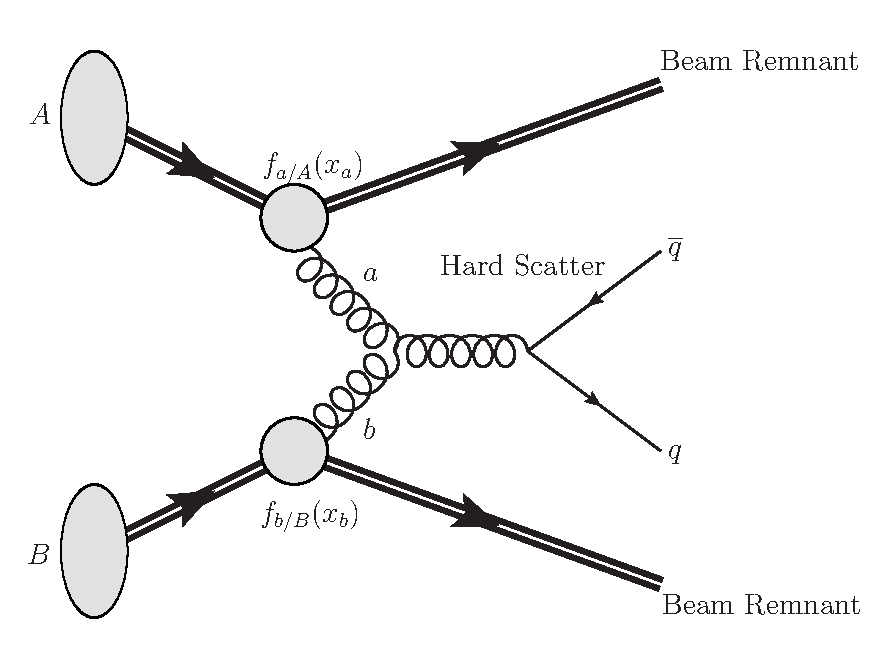
\includegraphics{figures/fd/pp.eps}}
	\caption{Schematic picture of a collision between two protons, labeled $A$ and $B$. Partons $a$ and $b$, which are gluons in this picture, participate in the hard scatter interaction, $gg\rightarrow q\overline{q}$. The beam remnants, the remainder of the two protons, do not participate in the hard scatter interaction, but can interact with the final state partons from the hard scatter interaction and with each other, forming the underlying event. The outgoing colored partons undergo fragmentation and hadronization to form jets, not shown here. }
	\label{fig:pp-collision}
\end{figure}


The PDFs are determined from fits to existing data; the dependence on $x$ must be determined from the data, while the dependence on the factorization scale can be derived from the DGLAP equations~\cite{Gribov:1972ri,Dokshitzer:1977sg,Altarelli:1977zs}. Uncertainties on the PDFs take into account the experimental uncertainties on the input data, as well as various assumptions used in the PDF extraction, such as the value of $\alpha_s$ used in the fit. An example is shown in figure~\ref{fig:theory-pdf-example}. At high $x$, the PDFs are dominated by the three valence quarks ($uud$), while at low $x$, gluons and sea quarks (quark-antiquark pairs formed from the splitting of a gluon) are more prominent. At higher energy scales, the sea quark distributions are more flavor-symmetric, and the gluon and sea quark distributions are larger with respect to the valence quarks.


\begin{figure}[htbp]
	\centering
	\hfill
	\subfloat[] {
		\resizebox{0.4\textwidth}{!}{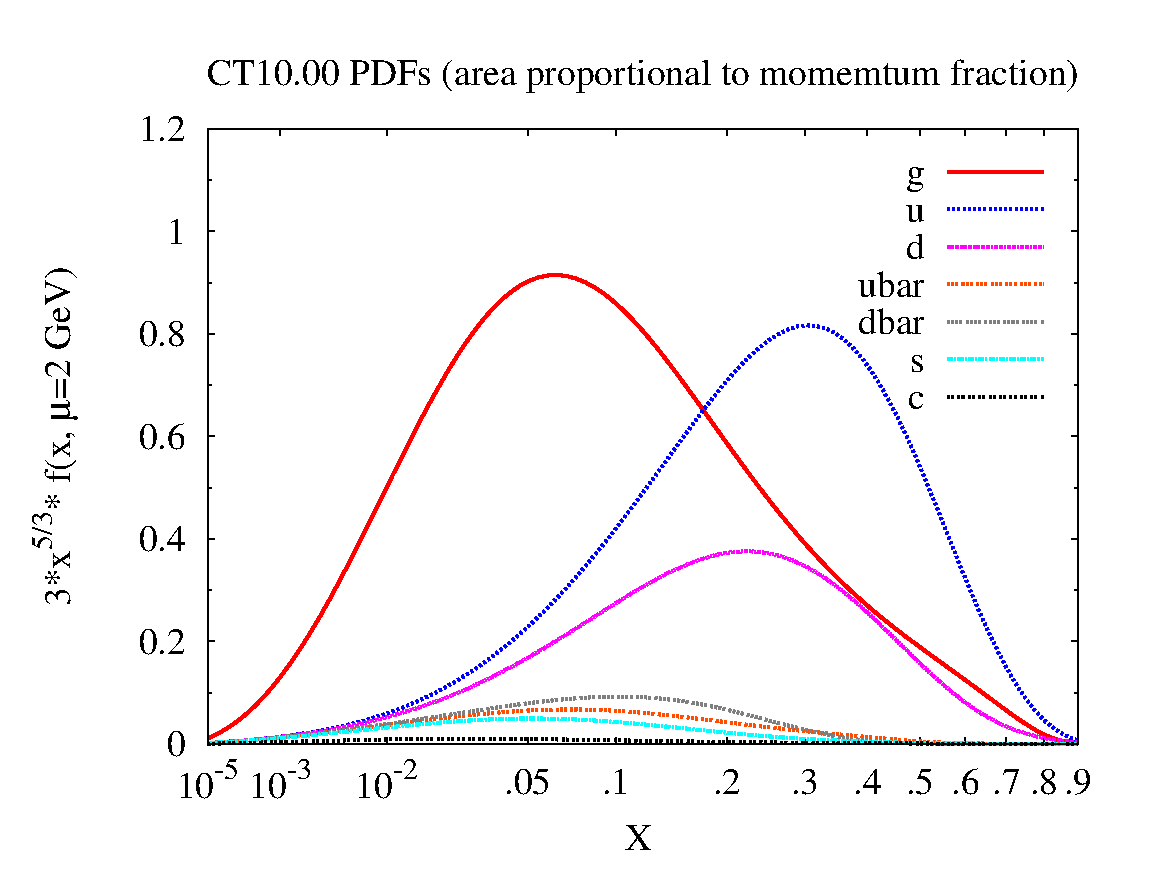
\includegraphics{figures/theory/pdf-ct10Q2a}}
	}
	\hfill
	\subfloat[] {
		\resizebox{0.4\textwidth}{!}{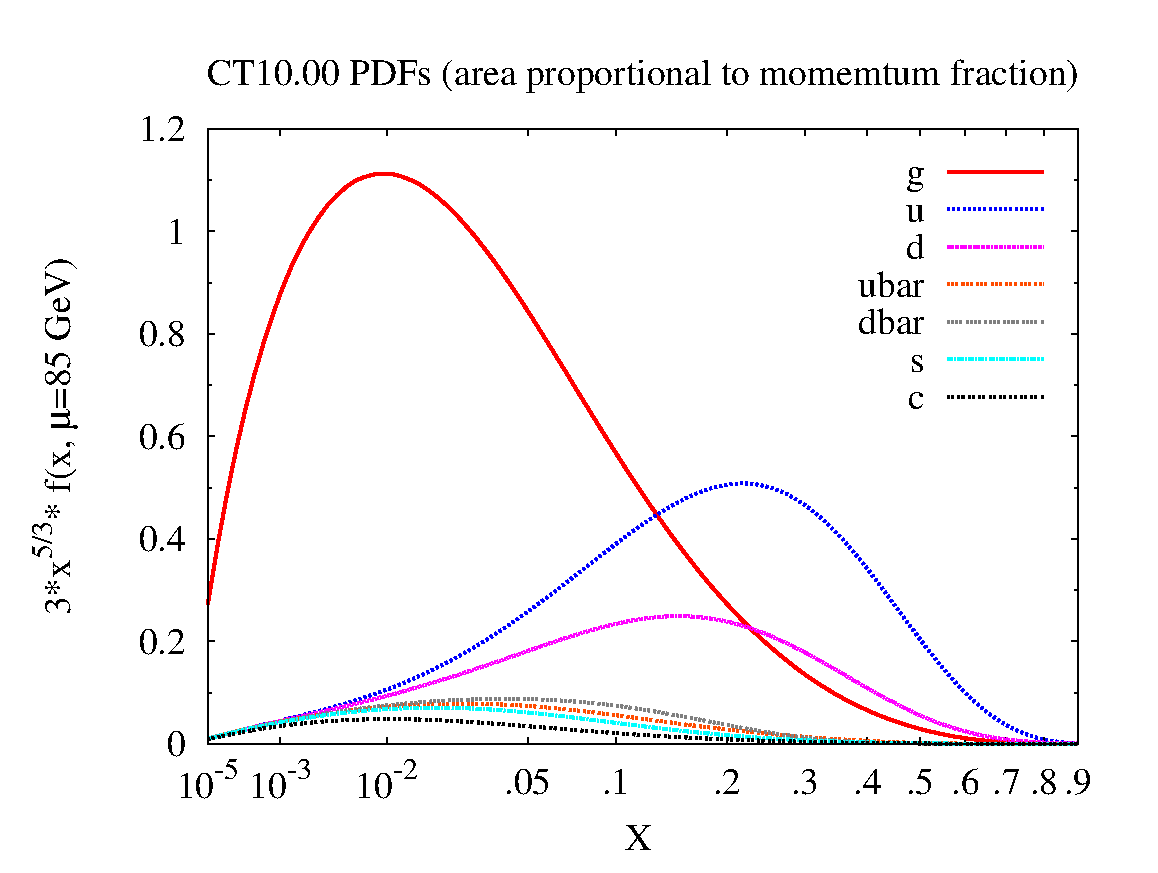
\includegraphics{figures/theory/pdf-ct10Q85a}}
	}
	\hfill
	\caption[Example parton distribution functions at $\mu=\SI{2}{\giga\electronvolt}$ and $\mu=\SI{85}{\giga\electronvolt}$, from the CT10 PDF set.]{Example parton distribution functions at $\mu=\SI{2}{\giga\electronvolt}$ and $\mu=\SI{85}{\giga\electronvolt}$, from the CT10 PDF set~\cite{ct10}.}
	\label{fig:theory-pdf-example}
\end{figure}

\subsubsection{Jets}
A typical proton-proton collision will typically produce several colored partons, from the hard scattering interaction itself or from QCD radiation from initial or final state partons. Free quarks are not observed in nature due to confinement, and hence the colored partons are not directly observed. Rather, the partons transform into a collection of color-neutral hadrons, which are observed as clusters of particles called \emph{jets}. Quarks and gluons emerging from the collision radiate additional gluons, and the gluons split into quark-antiquark pairs (\emph{fragmentation}). The splittings, which are dominated by the emission of soft and collinear radiation, continue until the local momentum scales reach $\mathcal{O}(\SI{1}{\giga\electronvolt})$, at which point QCD becomes strongly interacting and confines the partons into hadrons (\emph{hadronization}). 

The perturbative part of jet formation can be modeled using a \emph{parton shower} algorithm, which describes probabilistically the creation soft or collinear partons due to splittings~\cite{Buckley:2011ms}. Hadronization is a non-perturbative process, and hence cannot be computed from QCD. It is instead described by phenomenological models, such as the Lund string model~\cite{Andersson:1983ia} or the cluster model~\cite{Webber:1983if}, which incorporate many free parameters to tune to data. 


\subsection{Electroweak Sector}
The electroweak sector is a unified description of electromagnetism and weak decays as a gauge theory with gauge group $\mathrm{SU}(2)_L\times U(1)_Y$. The theory models a number of phenomena, including:
\begin{itemize}
	\item The weak decays of heavy quarks and leptons.
	\item The nonzero masses of the weak gauge bosons, quarks, and charged leptons.
	\item Flavor violation in weak decays involving charged currents.
	\item Violation of $C$-, $P$-, and $CP$-symmetry observed in certain decay processes~\cite{Wu:1957my,Christenson:1964fg,Collaboration:1999jz,AlaviHarati:1999xp}.
\end{itemize}

The underlying theory of the electroweak sector is rather more complicated than the strong sector. $C$ violation is manifest in the construction of the theory: the gauge couplings are \emph{chiral}, with the left- and right-handed components of fermions belonging to different representations of $\mathrm{SU}(2)$. Such a symmetry forbids mass terms for the fermions and gauge bosons, in clear conflict with observations. To accommodate fermion and gauge boson masses without abandoning the symmetry, a scalar Higgs field is added with a quartic potential arranged such that the ground state spontaneously breaks the $\mathrm{SU}(2)_L$ symmetry. The resulting theory contains a large number of free parameters: two gauge couplings $g$ and $g'$, two constants in the quartic Higgs potential, nine Yukawa couplings between the fermions and the Higgs field, and three mixing angles and one phase in the CKM matrix. 

%The Lagrangian can be broken into two pieces, $\mathcal{L} = \mathcal{L}_{\mathrm{sym}} + \mathcal{L}_{\mathrm{Higgs}}$, where the first piece contains terms with only gauge bosons and fermion fields and conserves $\mathrm{SU}(2)_L$ symmetry, and the second piece contains terms with Higgs fields and spontaneously breaks $\mathrm{SU}(2)_L$ symmetry. 

In the this and the following sections, $W^{a\mu}$ represents the three $\mathrm{SU}(2)_L$ gauge fields, $B^{\mu}$ the $\mathrm{U}(1)_Y$ gauge field, and $\phi$ the Higgs scalar field, which is a complex $\mathrm{SU}(2)_L$ doublet. Assigning the left-handed components of fermions to the doublet $\mathrm{SU}(2)_L$ representation and the right-handed components to the singlet presentation, the Standard Model quarks are denoted by $Q_L^i\equiv \left(\begin{array}{c} u^i_L \\ d^i_L \end{array}\right)$, $u_R^i$, and $d_R^i$, where $i=1,2,3$ indicates the generation. Similarly, the leptons are denoted by $E_L^i\equiv \left(\begin{array}{c} \nu_L^i \\ e_L^i \end{array}\right)$ and $e_R^i$. There is no corresponding right-handed neutrino in the theory. 

\subsubsection{The Higgs Mechanism}\label{sec:higgs-mechanism}
Much of the phenomenology of the electroweak sector can be derived starting from the observation that the $W^{\pm}$ and $Z^0$ bosons have masses of nearly $\SI{100}{\giga\electronvolt}$, as heavy as entire krypton or molybdenum atoms. Straightfowardly adding explicit gauge boson masses in the Lagrangian, e.g. $m_W^2 (W_{\mu}^a)^2$, fails immediately  due to the requirement of gauge invariance. It is easy to see that such terms in not invariant under equation~\ref{eqn:gauge-field-transformation-infinitesimal}.

% , inspired by developments in superconductivity in the early 1960s~\cite{Nambu:1960tm + anderson?},
The solution to this quandary is that the ground state of the theory need not exhibit the same symmetries as the underlying Lagrangian. This phenomenon, known as spontaneous symmetry breaking, underlies the Higgs mechanism~\cite{Higgs:1964pj,Englert:1964et,Guralnik:1964eu}, and is realized in the model of Glashow, Salam, and Weinberg~\cite{Glashow:1961tr,Weinberg:1967tq,Salam:1968rm}. 

The model introduces an $\mathrm{SU}(2)$ doublet of scalar fields, $\phi$, with Lagrangian,


\begin{equation}\label{eqn:higg-lagrangian}
	\mathcal{L}_{\mathrm{Higgs}} = |D_{\mu}\phi|^2 - V(\phi^{\dagger}\phi),
\end{equation}

where the potential energy term given by:
\begin{equation}\label{eqn:higgs-potential}
	V(\phi^{\dagger}\phi) = \frac12 \mu^2 \phi^{\dagger}\phi + \frac14 \lambda (\phi^{\dagger}\phi)^2.
\end{equation}


The quartic potential induces electroweak symmetry breaking if the quadratic coefficient is negative, i.e. $\mu^2<0$. The potential is then minimized for a nonzero value of $\phi$. Using the $\mathrm{SU}(2)_L$ symmetry, we can take vacuum expectation value of $\phi$ to be:

\begin{equation}
	\langle \phi \rangle = \frac{1}{\sqrt{2}} \left(\begin{array}{c} 0 \\ v \end{array}\right).
\end{equation}
 
Solving for $v$,

\begin{align}
	0 = \frac{\mathrm{d}V}{\mathrm{d}v} &= -\frac12\mu^2 v + \frac14\lambda v^3 \\
	v &= \frac{2\mu^2}{\lambda}.
\end{align}

Expanding the Higgs field about its expectation value, $\phi$ can be written:

\begin{equation}
	\phi = U \frac{1}{\sqrt{2}} \left(\begin{array}{c} 0 \\ v+H \end{array}\right),
\end{equation}

where $U$ is a local $\mathrm{SU}(2)$ gauge transformation that can be set to $\mathbf{1}$ by choice of gauge. 

The masses and interactions of various particles are described by expanding the Higgs field about $\langle \phi \rangle$ and identifying the relevant physical states. For the Higgs field itself, the potential energy terms are:

\begin{equation}
	\Delta \mathcal{L} = -\frac12 m_H^2 H^2 - \sqrt{\frac{\lambda}{2}} m_H H^3 - \frac14 \lambda H^4,
\end{equation}

 where $m_H=\sqrt{2}\mu$. The theory thus predicts a massive scalar boson with cubic and quartic self interactions.


\subsubsection{Gauge Bosons}
The mass terms for the gauge bosons arise from the covariant derivative terms in equation~\ref{eqn:higg-lagrangian}. Expanding the covariant derivatives, the relevant mass terms are:

\begin{equation}
	\Delta\mathcal{L} = \frac{1}{8} v^2 \left( g^2 (W^1_{\mu}W^{1\mu} + W^2_{\mu}W^{2\mu}) + (g'B_{\mu} - gW^3_{\mu})^2 \right).
\end{equation}

The physical states are the gauge- and mass-eigenstates,
\begin{align}
	W^{\pm}_{\mu} &= \frac{W^1 \mp iW^2}{\sqrt{2}} \label{eqn:weak-diag-W} \\
	Z^0_{\mu} &= -\sin\theta_w B_{\mu} + \cos\theta_w W_{\mu}^3 \label{eqn:weak-diag-Z}\\
	A_{\mu} &= \cos\theta_w B_{\mu} + \sin\theta_w W_{\mu}^3\label{eqn:weak-diag-A},
\end{align}

where $\tan\theta_w = \frac{g'}{g}$. The corresponding masses are:
\begin{align}
	m_{W^{\pm}} &= \frac{gv}{2} \\
	m_{Z^0} &= \frac{gv}{2\cos\theta_w} \\
	m_{A} &= 0.
\end{align}

The theory thus predicts a nontrivial relationship between the masses of the gauge bosons, $m_{W^{\pm}}$ and $m_{Z^0}$, and the gauge coupling constants $g$ and $g'$.

In addition to the Higgs terms in equation~\ref{eqn:higg-lagrangian}, the Standard Model Lagrangian contains the pure gauge term shown in equation~\ref{eqn:simple-gauge-lagrangian}, 

\begin{equation}
	\Delta\mathcal{L} = -\frac14(F^a_{\mu\nu})^2,
\end{equation}

where $F_{\mu\nu}^a$ is the field strength tensor (equation~\ref{eqn:field-strength-tensor}). The structure constants are given by $f^{abc}=i\epsilon^{abc}$, where $\epsilon^{abc}$ is the Levi-Civita symbol. In addition to the quadratic kinetic term for the electroweak gauge bosons, the Lagrangian contains cubic and quartic terms, which correspond to interactions between three or four bosons: $WWZ$, $WW\gamma$, $WWWW$, $WWZZ$, $WW\gamma\gamma$, and $WWZ\gamma$. 


\subsubsection{Fermion Masses}\label{sec:standard-model-fermion-masses}
The fermion masses arise from the Yukawa coupling terms between the fermions and the Higgs field,
\begin{equation}\label{eqn:lagrangian-yukawa-couplings}
	-\Delta \mathcal{L} = - \left(\lambda_d^{ij} \overline{Q}_L^i \cdot \phi d_R^j - \lambda_u^{ij} \epsilon^{ab}\overline{Q}^i_{La} u_R^j + \mathrm{h.c.}\right) - \left(\lambda_l^{ij} \overline{E}^i_L \cdot \phi e_R^j + \mathrm{h.c.}\right).
\end{equation}
 
 The $\lambda_{u,d,l}^{ij}$ are complex matrices of coupling constants. These are, in general, not symmetric or Hermitian, and to identify the physical mass eigenstates, the matrices must be diagonalized. The Yukawa matrices can be decomposed using the singular value decomposition as:

\begin{equation}
	\lambda_u = U_u D_u W_u^{\dagger},\ \lambda_d = U_d D_d W_d^{\dagger},\ \lambda_l = U_l D_l W_l^{\dagger},
\end{equation}
 
where $U_{u,d,l}$ and $W_{u,d,l}$ are unitary matrices, and $D_{u,d,l}$ are diagonal, non-negative matrices. Making a change of variables,

\begin{align}\label{eqn:yukawa-diagonalization}
	u_L^i\rightarrow U_{u}^{ij}u_L^j&,\ d_L^i\rightarrow U_d^{ij}d_L^j, \\
	u_R^i\rightarrow W_{u}^{ij}u_R^j&,\ d_R^i\rightarrow W_d^{ij}d_R^j, \\
	e_L^i\rightarrow U_l^{ij}e_L^j&,\ \nu_L^i\rightarrow U_l^{ij}\nu_L^j, \\
	e_R^i\rightarrow W_l^{ij}e_R^j&,
\end{align}

the off-diagonal Yukawa couplings vanish as intended, while the kinetic terms remain invariant. The masses of the fermions are:

\begin{equation}
	m_u^i = \frac{1}{\sqrt{2}} D_u^{ii}v,\ m_d^i = \frac{1}{\sqrt{2}} D_d^{ii}v,\ m_l^i = \frac{1}{\sqrt{2}} D_l^{ii}v,\ m_{\nu}^i = 0.
\end{equation}


\subsubsection{Electroweak Interactions of Fermions}
The Lagrangian describing the interactions of fermions and gauge bosons is:

\begin{equation}\label{eqn:electroweak-lagrangian}
	\mathcal{L}_{\mathrm{sym}} =  -\frac{1}{4} \sum_{i=1}^3  \overline{E}_L (i\slashed{D}) E_L + \overline{e}_R(i\slashed{D})e_R + \overline{Q}_L(i\slashed{D})Q_L + \overline{u}_R(i\slashed{D})u_R+\overline{d}_R(i\slashed{D})d_R,
\end{equation}

where, similarly to equation~\ref{eqn:covariant-derivative-qcd}, the covariant derivative $D_{\mu}$ is given by:

\begin{align}\label{eqn:covariant-derivative-ew}
	D_{\mu} &= \partial_{\mu} - i g \tau^a W^{a}_{\mu} - i g' Y B_{\mu}, \\
\end{align}

where the $\tau^a$ are operators corresponding to the action of a given generator of the $\mathrm{SU}(2)_L$ Lie algebra, and $Y$ is an operator corresponding to the action of the generator of $\mathrm{U}(1)_Y$, which simply returns the hypercharge. For the left-handed doublets in the fundamental representation of $\mathrm{SU}(2)_L$, the $\tau^a$ can be taken to be the Pauli matrices, $\tau^a=\frac12 \sigma^a$. For right-handed singlets in the trivial representation of $\mathrm{SU}(2)_L$, the $\tau^a$ are zero. In other words, the right-handed fermions do not interact with the $W^{a\mu}$. 

In terms of the physical gauge bosons, given in equations~\ref{eqn:weak-diag-W}--\ref{eqn:weak-diag-A}, 
\begin{align}
	D_{\mu} &= \partial_{\mu} - i \frac{g}{\sqrt{2}}\left(W_{\mu}^+ \tau^+ + W_{\mu}^- \tau^-\right) - i\frac{g}{\cos\theta_w} Z_{\mu}\left(\tau^3 - \sin^2\theta_w Q\right) - i e A_{\mu} Q,
\end{align}

where $e=\frac{gg'}{\sqrt{g^2+g'^2}}$, $\tau^{\pm}=\left(\tau^1 \pm i \tau^2\right)$, and $Q=\tau^3+Y$. 

The fermion couplings to the gauge bosons are complicated by the fact that the mass eigenstates do not necessarily coincide with the gauge eigenstates, due to the off-diagonal Yukawa couplings in section~\ref{sec:standard-model-fermion-masses}. The diagonalization procedure alters the couplings of the quarks to the $W^{\pm}$ bosons. The quark-$W^{\pm}$ couplings can be written in terms of the current $J^{\mu\pm}=\sum_{i} \frac1{\sqrt{2}}\left(\overline{u}_L^i\gamma^{\mu}d_L^i\right)$ as:

\begin{equation}
	\Delta\mathcal{L} = g (W^+_{\mu}J^{\mu+}_W + W^{-}_{\mu}J^{\mu -}_{W})
\end{equation}

Under the transformation in equation~\ref{eqn:yukawa-diagonalization}, $J^{\mu\pm}\rightarrow \sum_{ij}\frac{1}{\sqrt{2}} \overline{u}_L^i \gamma^{\mu} V^{ij} d_L^j$, where $V^{ij}$ is a $3\times 3$ unitary matrix known as the \emph{Cabibbo-Kobayashi-Maskawa} (CKM) matrix, $V = U_{u}^{\dagger} U_d$. The non-zero off-diagonal elements of $V$ imply that weak decays mix the three generations of quarks; quark flavor is not conserved in weak decays, as is readily observed in hadron decays, e.g. $K^{\pm}\rightarrow \pi^{\pm}+\pi^0$. Further, $V$ contains one nontrivial complex phase, allowing for $CP$ violation in weak decays. Note that the lepton sector does not contain an analogous mixing matrix for weak decays, due to the presence of only a single Yukawa matrix $\lambda^{ij}_l$. Hence lepton flavor and $CP$ are conserved in leptonic weak decays.

The decays of $W^{\pm}$ and $Z^0$ bosons are shown in table~\ref{table:theory-WZ-BR}. Approximately $33\%$ of $W^{\pm}$ bosons decay to a lepton plus a neutrino. The branching fraction of the $Z^0$ boson to a lepton-antilepton pair is roughly $10\%$. In both cases, the decays are distributed nearly equally between the three lepton flavors. 

\begin{table}[htbp]
       \centering
       \hfill
       \subfloat[ $W$] {
               \begin{tabular}{cc}
                       \ \\
                       Decay & Branching Fraction \\
                       \hline
                       $e\nu$  &       $10.71\pm 0.16\ [\%]$ \\
                       $\mu\nu$        &       $10.63\pm 0.15\ [\%]$ \\
                       $\tau\nu$       &       $11.38\pm 0.21\ [\%]$ \\
                       Hadrons         &       $67.41\pm 0.27\ [\%]$ \\ 
                       \ 
               \end{tabular}
       }
       \hfill
       \subfloat[ $Z$] {
               \begin{tabular}{cc}
                       Decay & Branching Fraction \\
                       \hline
                       $e^+e^-$                &       $3.363 \pm 0.004\ [\%]$ \\
                       $\mu^+\mu^-$    &       $3.366 \pm 0.007\ [\%]$ \\
                       $\tau^+\tau^-$  &       $3.370 \pm 0.008\ [\%]$ \\
                       Invisible               &       $20.00 \pm 0.06\ [\%]$ \\
                       Hadrons                 &       $69.91 \pm 0.06\ [\%]$ \\
                       $4\ell$ ($\ell=e,\mu$)  &       $(3.20\pm0.28)\times10^{-6}$~\cite{TheATLASCollaboration:2014db} \\
               \end{tabular}
       }
       \hfill
       \caption[Branching fractions of $W^{\pm}$ and $Z^0$ bosons to leptons and other final states.]{Branching fractions of $W^{\pm}$ and $Z^0$ bosons to leptons and other final states~\cite{pdg}.}
       \label{table:theory-WZ-BR}
\end{table}


\section{Beyond the Standard Model}\label{sec:bsm}
Though quite successful as a description of most observed phenomena in particle physics, the Standard Model is deficient in several ways. Several observations indicate that the particle content is incomplete; additionally, the theory has a few unsatisfying constructional aspects which, while not technically inconsistent, suggest that there remains underlying physics to be discovered. Many theories have been proposed to solve these issues, and confronting these theories is a major goal of the ATLAS experiment. This section describes the motivations for searching for physics beyond the Standard Model (BSM), and lists several of the leading BSM theories which can be confronted at the LHC.

\subsection{Shortcomings of the Standard Model}\label{sec:bsm-unexplained-phenomena}

Several observations over the last few decades, largely from astrophysics and cosmology, are not described by the Standard Model. These include:

\begin{itemize}
	\item \textbf{Neutrino mass}: Due to the lack of right-handed neutrinos and left-handed antineutrinos, neutrinos are massless in the Standard Model. However, observation of neutrino flavor oscillations indicate that at least two of the three neutrinos have nonzero mass. The phenomenon of oscillation was first observed by the Homestake solar electron neutrino detector~\cite{Cleveland:1998nv}, in the form of a deficit of electron neutrinos detected from the sun. Later experiments observed oscillation among other types of neutrinos and antineutrinos, from a variety of sources including the sun, nuclear reactors, cosmic rays interacting with the atmosphere, and particle accelerators~\cite{pdg}. The data imply that the three neutrino mass eigenstates have different masses, with differences given by:
	\begin{align}\label{eqn:neutrino-mass-differences}
		|\Delta m_{21}^2| &\cong 7.5\times 10^{-5}~\mbox{eV}^2 \\
		|\Delta m_{31}^2| &\cong 2.5\times 10^{-3}~\mbox{eV}^2.
	\end{align}
	These relations hold only if at least two of the neutrino masses are nonzero. On the other hand, $\beta$-decay experiments and cosmological observations indicate an upper bound on the neutrino mass scale of order $m_{v_i} \lesssim \mathcal{O}(0.1-\SI{1}{\electronvolt})$~\cite{Aseev:2011ia, Abazajian:2011ck, Ade:2013zuv}.

	\item \textbf{Dark matter}: Astrophysical observations suggest the existence of a large amount of non-Standard Model matter which interacts only gravitationally with baryonic matter. The earliest tension with known physics comes from galactic rotation curves, the distribution of rotational velocities of stars about the galactic center as a function of radius~\cite{1980ApJ_238_471R}. The rotational velocities $v(r)$ can be compared with the expectation from the observed matter distribution, $\tilde{v}(r)=\sqrt{\frac{M(r)}{r}}$, where $M(r)$ is the observed mass at radius less than $r$. At large distances from the galactic center, the observed rotation curve behaves like $v(r)\sim$constant, while the expected rotation curves behaves like $v(r)\sim \frac{1}{\sqrt{r}}$. 

	At present, the leading explanation for the discrepancy is the presence of a large amount of gravitationally interacting, non-luminous matter in galaxies, known as \emph{dark matter}. The hypothesis is supported by cosmological observations: measurements of anisotropies in the cosmic microwave background (CMB) are sensitive to the relative amounts of baryonic matter (which interacts with photons), dark matter (which does not), and dark energy. A recent combination of CMB measurements gives the following values~\cite{Ade:1530686}:
	\begin{align}
		\Omega_{c}h^2 &= 0.1198 \pm 0.0026, \\
		\Omega_{b}h^2 &= 0.02207 \pm 0.00027, \\
		\Omega_{\Lambda} &= 0.685^{+0.017}_{-0.016}, \\
	\end{align}
	where $\Omega_{c}$ and $\Omega_{b}$ are the density parameters for cold dark matter and baryonic matter, respectively, $h$ is the Hubble constant, and $\Omega_{\Lambda}$ is the cosmological constant. 

	Many candidates have been proposed as the constituents of dark matter, such as primordial black holes, sterile neutrinos, axions, and weakly interacting massive particles (WIMPs). WIMPs are a particularly interesting candidate for LHC phenomenology: in the so-called ``freeze-out'' model of dark matter evolution, $\Omega_c$ is fixed when dark matter falls out of thermal equilibrium with conventional matter. $\Omega_c\sim0.1$ is achieved with $m_{\chi}\sim \mathcal{O}(100~\mbox{GeV})$ and couplings of order $g_X\sim\mathcal{O}(0.1-1)$; such a particle could be produced and detected at the LHC. 

	\item \textbf{Matter-Antimatter Asymmetry}: The observable universe is made up of matter and photons, with very little antimatter. Astrophysical observations measure the ratio of baryons (minus antibaryons) to photons,
	\begin{equation}\label{eqn:baryon-photon-ratio}
		\eta \equiv \frac{n_B - n_{\overline{B}}}{n_{\gamma}}, 
	\end{equation}
	to be in the range $5.7\times 10^{-10} \leq \eta \leq 6.7\times 10^{-10}$ at $95\%$ confidence level~\cite{pdg}. However, assuming symmetrical initial conditions and conservation of baryon number, the Big Bang would produce baryons and antibaryons in equal number\footnote{Asymmetric initial conditions are disfavored due to inflation, which would dilute any initial asymmetry~\cite{Cline:2006ts}.}. Due to inefficient annihilation after freeze-out, the present abundances would be $\frac{n_B}{n_{\gamma}} = \frac{n_{\overline{B}}}{n_{\gamma}} \approx 10^{-20}$~\cite{Cline:2006ts}. The generation of a large baryon-antibaryon asymmetry is known as the \emph{baryogenesis} problem.

	%Three conditions are necessary for baryogenesis, known as the Sakharov conditions~\cite{sakharov}: baryon number violation, $C$- and $CP$-symmetry violation, and interactions out of thermal equilibrium (i.e. the interaction rate must be slower than the expansion rate of the universe). In principle, the Standard Model possibly satisfies all three conditions: baryon number is violated by electroweak sphaelerons~\cite{thooft}, $C$ and $CP$ violation is observed in hadron oscillations and decays~\cite{Kindirect, Kdirect,B,D}, and thermal equilibrium may be lost if the electroweak phase transition is sufficiently first-order~\cite{???}. However, baryogenesis of sufficient magnitude has not been demonstrated, in particular due to insufficient $CP$-violation. 

	\item \textbf{Gravity}: Gravity is not described by the Standard Model. 

\end{itemize}

\subsection{Theoretical Issues}\label{sec:bsm-theoretical-deficiencies}
Besides not describing the phenomena listed above, the Standard Model has a number of theoretical issues related to its parameters and structure.

\begin{itemize}
	\item \textbf{Hierarchy problem}: The hierarchy problem refers to the large discrepancy between the electroweak scale, $\mathcal{O}(\SI{e2}{\giga\electronvolt})$, and the Planck scale, $\mathcal{O}(\SI{e19}{\giga\electronvolt})$. Due to fermion and gauge boson loops like those shown in figure~\ref{fig:higgs-mass-feyman-diagrams}, the Higgs boson mass receives quantum corrections proportional to $\Lambda^2$, where $\Lambda$ is the scale up to which the theory is valid. For example, due to a fermion $f$ with Yukawa coupling $\lambda_f$, the physical Higgs mass at one loop order is:

	\begin{equation}\label{eqn:higgs-mass-divergence}
		m_{H,\mathrm{phys}}^2 \approx m_{H}^2 -\frac{|\lambda_f|^2}{8\pi^2} \Lambda^2,
	\end{equation}

	where $m_{H}^2$ is the bare Higgs mass parameter in the Lagrangian. In practice, the contribution from the top quark, with $\lambda_t\sim1$, dominates this expression. If $\Lambda$ is near the Planck scale, $\Lambda\sim\SI{e19}{\giga\electronvolt}$, then with $m_H(\mathrm{phys})=\SI{125.1}{\giga\electronvolt}$, the bare Higgs mass and $\Delta m_H^2$ must cancel to some 30 orders of magnitude, an unsavory coincidence referred to as \emph{fine tuning}. Turning the problem on its head, if nature is not finely tuned, then $\Lambda$ should be not too far above the electroweak scale, $\Lambda \lesssim \SI{10}{\tera\electronvolt}$. The physics responsible for such a cutoff scale could be accessible at the LHC. 

	\begin{figure}[htbp]
		\centering
		\hfill
		\subfloat[] {
			\resizebox{0.4\textwidth}{!}{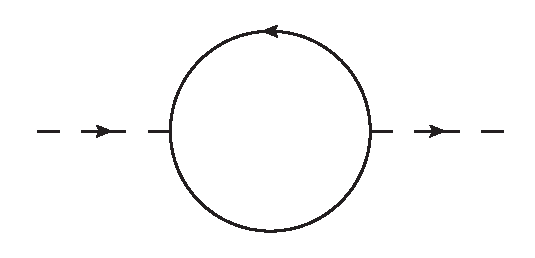
\includegraphics{figures/fd/Higgs_1loop_fermion}}
		}
		\hfill
		\subfloat[] {
			\resizebox{0.4\textwidth}{!}{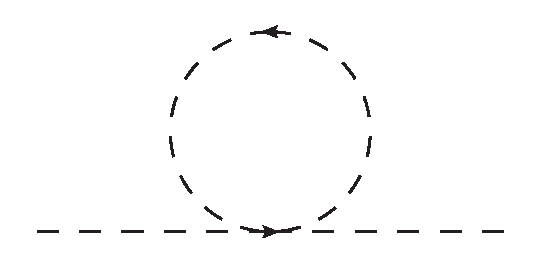
\includegraphics{figures/fd/Higgs_1loop_boson}}
		}
		\hfill
		\caption{One-loop Feynman diagrams involving fermions (left) and bosons (right) leading to the quadratic divergence of the Higgs mass.}
		\label{fig:higgs-mass-feyman-diagrams}
	\end{figure}
	

	\item \textbf{Strong $CP$ problem}: The strong sector of the Standard Model potentially contains a $CP$-violating term, 
	\begin{equation}
		\mathcal{L}_{\Theta}=\theta_{\mathrm{QCD}} \frac{\alpha_s}{8\pi}G^{\mu \nu a} \tilde{G}^{a}_{\mu\nu},
	\end{equation}
	where $-\pi\leq\theta_{\mathrm{QCD}}\leq\pi$ is the effective $\Theta$ parameter after diagonalizing the quark mass matrix, $G^{a}_{\mu\nu}=\partial_{\mu}\mathcal{A}_{\mu}^{a}-\partial_{\nu}\mathcal{A}_{\mu}^{a} - g_s f^{abc}\mathcal{A}_{\mu}^{b} \mathcal{A}_{\nu}^{c}$ is the gluon field strength tensor, and $\tilde{G}^a_{\mu\nu}=\epsilon_{\mu\nu\alpha\beta}G^{\alpha\beta a}$ is its dual~\cite{pdg}. However, this term is severely constrained by measurements of the neutron dipole moment~\cite{PhysRevLett.97.131801}, with a limit of $|\theta_{\mathrm{QCD}}|\lesssim 10^{-10}$. 

	Axions are a leading candidate for the resolution of the strong $CP$ problem~\cite{Peccei:400569}. These are typically very weakly coupled, and would not be observable at the LHC.

	\item \textbf{Free parameters}: The Standard Model contains 19 free parameters. In terms of measured quantities, these are the 6 quark masses $m_{q_i}$, 3 lepton masses $m_{l_i}$, 3 CKM mixing angles $\theta_{ij}$ and 1 CKM phase $\delta$, 3 gauge couplings $g_i$, the QCD vacuum angle $\theta_{\mathrm{QCD}}$, the Higgs field vacuum expectation value $v$, and the Higgs mass, $m_H$. These parameters are measured; their values are not predicted by the theory. It remains unknown why the Yukawa couplings range over six orders of magnitude, for example, nor why the fermions fall into three identical generations. A more complete theory might explain the patterns observed among the parameters and predict their values.


	\item \textbf{Gauge Unification}: The origin of the Standard Model gauge group, $G_{SM}=SU(3)_c\times SU(2)_L \times U(1)_Y$, is not understood. Remarkably, the Standard Model fermion content can be described as a $\mathbf{5}^{*}\oplus \mathbf{10}$ representation of $\mathrm{SU}(5)$, the smallest simple group containing $G_{SM}$, with all of the Standard Model quantum numbers correctly predicted. Unfortunately, simply augmenting the gauge group to $\mathrm{SU}(5)$ leads to an unacceptable rate of proton decay, but deriving $G_{SM}$ from a larger, ``unified'' gauge group remains a topic of active investigation.  
\end{itemize}

\subsection{Theories of BSM Physics}\label{sec:bsm-theories}
A large number of theories have been developed to address the problems in the previous section, many of which yield testable predictions for the LHC. This section describes three examples of such theories: supersymmetry, extra fermions beyond the three Standard Model generations, and the neutrino seesaw mechanism. These theories are capable of producing three or more charged leptons in $pp$ collisions through the production and decay of heavy new particles, and can thus be confronted against the analyses described in chapters~\ref{ch:model-independent-trilepton-search} and \ref{ch:trilepton-resonance-search}.

\subsubsection{Supersymmetry}
The hierarchy problem described above motivates the consideration of additional symmetries. Consider again the Higgs mass quadratic divergence (equation~\ref{eqn:higgs-mass-divergence}). The divergence could be avoided by introducing scalar partners to the fermions to counteract the divergence, due to the relative (-) sign between scalar and fermion loops in figure~\ref{fig:higgs-mass-feyman-diagrams}. Canceling the divergence at all orders suggests the introduction of an extra symmetry to the Standard Model. 

The forms that such a symmetry could take are quite restricted. In 1967, Coleman and Mandula demonstrated that, under a small set of physically assumptions, the symmetry algebra of the $S$-matrix must be isomorphic to a direct product of the Poincar\'{e} group and an internal symmetry group (i.e. whose generators commute with those of the Poincar\'{e} group). This \emph{no-go} theorem appeared to establish that it is impossible to ``[combine] space-time and internal symmetries in any but a trivial way.'' However, a loophole was found in 1975, formalized in the theorem of Haag, Lopuszanski, and Sohnius: the Poincar\'{e} group can be extended nontrivially in the context of graded Lie algebras, allowing the symmetry generators to be commuting or anticommuting~\cite{Haag1975257}. These so-called ``supersymmetries'', first proposed in by Wess and Zumino~\cite{Wess197439}, transform bosons to fermions and vice-versa, and combine nontrivially with the Poincar\'{e} group in that the anticommutator of two supersymmetry generators is a spacetime translation. 

By itself, supersymmetry predicts a partner for every Standard Model particle with identical mass and quantum numbers, except that the spin differs by 1/2. The symmetry is assumed to be spontaneously broken at some high mass scale, giving additional mass to the superpartners to account for the fact that superpartners have not yet been observed. The minimal implementation, called the \emph{minimal supersymmetric Standard Model} (MSSM), contains 178 free parameters, although simplifying assumptions are almost always used to reduce this enormous parameter space to manageable size.

Supersymmetry addresses a number of the shortcomings of the standard model described above. First, it provides a boson-fermion symmetry to cancel the quadratic divergence in the Higgs mass. Second, the superpartners are typically assigned an extra quantum number, $R$-parity, under with the SM particles are neutral, in order to stabilize the proton; this extra symmetry has the consequence of making the lightest supersymmetric particle (LSP) stable, providing a dark matter candidate. Third, the supersymmetry breaking sector contains numerous CP-violating parameters, which could provide the necessary CP violation to explain the matter-antimatter asymmetry in the universe. Finally, the superpartners modify the running of the three gauge couplings such that they approach similar values in the UV, supporting the notion of gauge unification. 

Trilepton events are a useful tool in MSSM searches. A common scenario is that the heavy supersymmetric particles decay back to Standard Model particles plus an LSP, often producing three or more leptons in the decay chains. Figure~\ref{fig:theory-susy-trilepton-example} shows an example involving the production of charginos and neutralinos, the superpartners of the $W^{\pm}$, $Z^0$, and $H$ bosons. ATLAS has performed several dedicated searches for such scenarios~\cite{TheATLASCollaboration:2014cs,Aad:2014ia,TheATLASCollaboration:2014hq}, which are not discussed in this dissertation. 

\begin{figure}[htbp]
	\centering
	\resizebox{0.4\textwidth}{!}{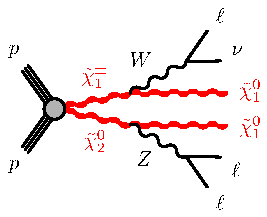
\includegraphics{figures/fd/C1N2-lllvN1N1-WZ}}
	\caption{Feynman diagram showing the production of a chargino, $\tilde{\chi}_1^{\pm}$, and a neutralino, $\tilde{\chi}^0_2$, decaying to two neutralino LSPs, $\tilde{\chi}^0_1$, plus three leptons and a neutrino. The chargino/neutralino subscript indicates mass ordering, with $1$ being the lightest.}
	\label{fig:theory-susy-trilepton-example}
\end{figure}



\subsubsection{Extra Generations of Matter}\label{sec:theory-bsm-vlf}
Given that the origin of the three generations of fermions is not understood, an obvious question is whether additional generations might exist. A review of extra fermions can be found at~\cite{Frampton:1999kr}. A fourth chiral generation, i.e. another copy of the three known generations, is strongly constrained, though not completely excluded~\cite{Buchkremer:2012gb,Djouadi:2012dm,Chanowitz:2013hk,Banerjee:2014gy}. The number of neutrinos coupling to the $Z$ boson with $m_{\nu}<\frac12 m_Z$ can be determined from the invisible width of the $Z$, giving $N_{\nu}= 2.9840 \pm 0.0084$. Further, additional chiral fermions coupling to the Higgs boson would significantly alter its production rate and decay patterns. In particular, an additional pair of quarks would increase the production cross section for $gg\rightarrow H$ by roughly a factor of 9. 

Additional non-chiral, or \emph{vector-like}, fermions are less constrained. Such fermions are defined as having identical left- and right-handed interactions under the Standard Model gauge group, particularly under $\mathrm{SU}(2)_L$. Consequently, explicit mass terms, $m\overline{\psi}\psi$, are not forbidden by gauge invariance, and the fermions need not couple to the Higgs field to acquire mass. The impact on Higgs production and decay, as well as precision electroweak observables, are small. Further, the pattern of extra vector-like fermions is less restricted compared to chiral generations, where a spectacular cancellation between the fields of each generation is needed to avoid chiral anomalies~\cite{Geng:1988pr}. 

Vector-like fermions are a feature of many model of BSM physics. Additional quarks are present in some models addressing the hierarchy problem, such as the little Higgs model~\cite{Arkani-Hamed:557546} or composite Higgs models~\cite{Kaplan:148688}. Vector-like leptons can appear alongside quarks in $\mathrm{SU}(5)$ multiplets~\cite{Martin:2012dx}, and are predicted in models explaining the fermion mass hierarchy~\cite{Falkowski:2014hs}, composite Higgs models, models with warped extra dimensions~\cite{Redi:2013ib,Contino:1005586}, and the type~III neutrino seesaw mechanism, discussed in section~\ref{sec:theory-bsm-seesaw}. 

In order to render the vector-like fermions unstable, mixing terms involving the Standard Model fermions can be introduced. This enables decays to a $W^{\pm}$, $Z^0$, or $H$ boson, plus a Standard Model quark or lepton. Three or more leptons can be produced if the bosons decay leptonically. In the case of vector-like leptons, the three leptons can also be produced resonantly, allowing the use of a trilepton mass constraint. An example Feynman diagram is shown in figure~\ref{fig:theory-heavy-lepton-feynman-diagrams-cc}. The collider phenomenology of vector-like leptons is discussed in more detail in section~\ref{sec:resonance-signal-models}.

\begin{figure}[htbp]
	\centering
	\resizebox{0.51\textwidth}{!}{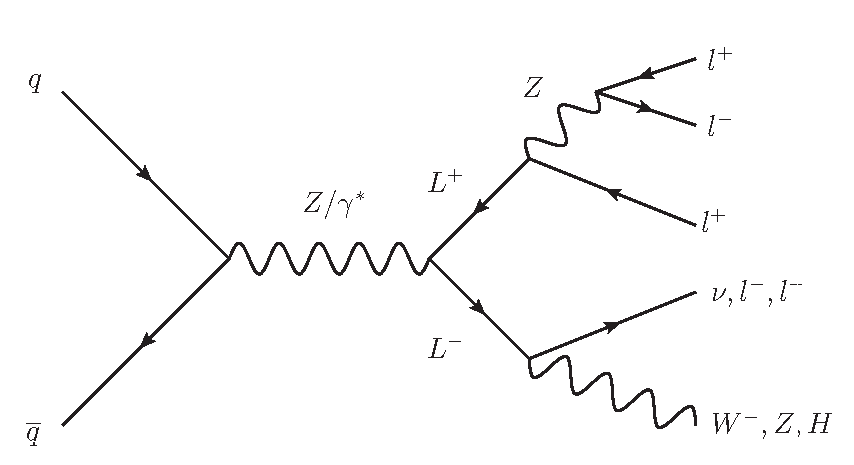
\includegraphics{figures/resonance/fd_cc2.eps}}
	\caption{Example of the pair production of two vector-like leptons, $\lpm$. The $L^{\pm}$ decay via mixing with Standard Model leptons. In this example, one vector-like lepton is shown decaying to three leptons via an intermediate $Z$ boson.}
	\label{fig:theory-heavy-lepton-feynman-diagrams-cc}
\end{figure}

\subsubsection{Neutrino Seesaw}\label{sec:theory-bsm-seesaw}
Due to the lack of right-handed neutrinos in the Standard Model, neutrinos are exactly massless. A neutrino mass term, $m_{\nu} \overline{\nu}_L \nu_L^c$ violates $\mathrm{SU}(2)_L$ gauge invariance. An effective mass term arising perturbatively, e.g. $\frac{Y_{ij}}{v}\phi\phi L_i L_j$, would be a good candidate to explain the small size of neutrino masses due to suppression from the mass scale $v$, but turns out to be forbidden as well due to the accidental conservation of lepton number, $L$, and also baryon minus lepton number, $B-L$~\cite{RevModPhys.75.345}. 

If neutrinos are their own antiparticle, i.e. are Majorana fermions rather than Dirac fermions, a leading candidate to explain the small but nonzero neutrino masses is the \emph{neutrino seesaw mechanism}~\cite{Mohapatra:1980yp,GellMann:1980vs,Yanagida:1980xy}. The Standard Model is augmented with heavy, sterile neutrinos, $N_i$, which have both Majorana masses and Yukawa interactions with the Standard Model neutrinos:
\begin{equation}
	\mathcal{L}_N = \frac12 M_{N_{ij}} \overline{N}^c_i N_j + Y_{ij}^{\nu} \overline{L}_{i} \tilde{\phi} N_{j} + \mathrm{h.c.}
\end{equation}

where $L_i = \left(\begin{array}{c}\nu_i \\ \ell_i \end{array}\right)$. The resulting mass matrix takes the form:

\begin{equation}
	M_{\nu} = \left(\begin{array}{cc} 0 & Y^{\nu} \frac{v}{\sqrt{2}} \\ (Y^{\nu})^T \frac{v}{\sqrt{2}} & M_N \end{array}\right)
\end{equation}
in the basis $\left(\begin{array}{c} \nu_{i} \\ N_j \end{array} \right)$. If $M_N \gg v$, then diagonalizing the mass matrix gives three eigenstates will light masses, $m_{\nu_{L_i}} \sim  \frac{Yv^2}{M_N}$. With $v=246~\mbox{GeV}$, a light neutrino mass of $m_{\nu}=0.1~\mbox{eV}$ gives a heavy neutrino mass of:
\begin{equation}
	M_N \sim Y \times 10^{15}~\mbox{GeV}.
\end{equation}

Hence Yukawa couplings of order 1 predict heavy, sterile neutrinos around the GUT scale, while smaller couplings predict a proportionally smaller mass scale. New mass scales accessible at the LHC can be achieved with more complicated models, such as the inverse seesaw model~\cite{Deppisch:2005ky}, which introduce more mass scales and high powers of the suppression factors.

At tree level, there are three possible implementations of the seesaw mechanism: 
\begin{itemize}
	\item \textbf{Type I}: The simplest realization of the seesaw mechanism, at least two sterile neutrinos $N_i$ are introduced as described above. This scenario is not likely to be testable at the LHC, due to the combination of small Yukawa couplings and large sterile neutrino masses required for $\mathcal{O}(0.1~\mbox{eV})$ neutrino masses. 

	\item \textbf{Type II}: The seesaw mechanism is generated by an $\mathrm{SU}(2)_L$ triplet of scalars, $\Delta$, with hypercharge $Y=2$. This allows the construction of the following Yukawa term:
	\begin{equation}
		-\mathcal{L} = Y^{\Delta}_{ij} L_{i}^T C \sigma_2 \Delta L_{j} + \mathrm{h.c.},
	\end{equation}
	where $i$ ranges over the three lepton flavors.  Assuming diagonal Yukawa couplings for simplicity, the neutral component of the triplet, $\Delta^0$, acquires a vacuum expectation value,
	\begin{equation}
		v_{\Delta} = \frac{\mu v^2}{\sqrt{2} m_{\Delta}^2},
	\end{equation}
	where $m_{\Delta}$ is the mass term for $\Delta$, $\mu\sim m_{\Delta}$ is a coefficient of the cubic Higgs-$\Delta$ interaction with mass dimension 1, and $v$ is the Standard Model Higgs vacuum expectation value. The light neutrinos acquire mass:
	\begin{equation}
		m_{\nu_{i}} \sim Y^{\Delta}_{i} v_{\Delta}=Y^{\Delta}_{i} \frac{\mu v^2}{\sqrt{2} m_{\Delta}^2}.
	\end{equation}

	The triplet of scalars can potentially be produced via gauge interactions at the LHC, if their masses are below the TeV scale. The new particle content consists of $\Delta^0$, $\Delta^{\pm}$, and $\Delta^{\pm\pm}$. Same-sign dilepton final states have been used to search for the doubly charged scalar~\cite{TheATLASCollaboration:2015gu}, and $\Delta^{\pm\pm}\Delta^{\mp\mp}$ pair production is used as a benchmark model for the model-independent trilepton search presented in chapter~\ref{ch:model-independent-trilepton-search}. 


	\item \textbf{Type III}: The seesaw mechanism is generated by at least two $\mathrm{SU}(2)_L$ triplets of fermions with hypercharge $Y=0$,
	\begin{equation}
		\Sigma = \Sigma^a \sigma^a = \left(\begin{array}{cc} \Sigma^0/\sqrt{2} & \Sigma^+ \\ \Sigma^- & -\Sigma^0/\sqrt{2} \end{array}\right). 
	\end{equation}
	The Lagrangian is:
	\begin{equation}
		\mathcal{L}_{\Sigma} = \mathrm{Tr}[i\overline{\Sigma}\slashed{D}\Sigma] - \frac12 \mathrm{Tr}[\overline{\Sigma}M_{\Sigma}\Sigma^c+\overline{\Sigma^c}M_{\Sigma}^{*}\Sigma] - \tilde{\phi}^{\dagger}\overline{\Sigma}\sqrt{2}Y_{\Sigma}L - \overline{L}\sqrt{s}Y_{\Sigma}^{\dagger}\Sigma \tilde{\phi},
	\end{equation}
	where $L=(\nu,l)^T$, $\phi=(\phi^+, \phi^0)^T$, $\tilde{\phi}=i\sigma_2\phi^{*}$, and $\Sigma^c=C\overline{\Sigma}^T$. Summation over lepton flavor is implicit. The neutral fermion $\Sigma^0$ generates the seesaw mechanism in much the same way as in the type I implementation, giving neutrino masses:
	\begin{equation}
		m_{\nu} = -v^2 Y_{\Sigma}^T \cdot M_{\Sigma}^{-1} \cdot Y_{\Sigma}
	\end{equation}
	
	Like the scalar triplet, the heavy fermion triplet can also be produced at detectable rates at the LHC via gauge interactions. The collider phenomenology of the fermions, which are vector-like, is described in more detail in section~\ref{sec:resonance-signal-models}. 
\end{itemize}

\printbibliography
\chapter{The Experimental Apparatus}
\section{The Large Hadron Collider}
The Large Hadron Collider (LHC) is a particle accelerator designed to explore the physics of particles at the energy scale of electroweak symmetry breaking. The accelerator occupies a 26.7 km tunnel beneath the Switzerland-France border near Geneva, which previously housed the Large Electron Positron Collider (LEP). Protons are accelerated in two counter-rotating beams up to a design momentum of $7~\mbox{TeV}/c$. The beams collide at four interaction points (IPs), shown in figure~\ref{fig:LHC-IPs}, where four collider detectors, ATLAS, CMS, LHCb, and ALICE, analyze the remnants of the collisions.

\begin{figure}[htbp]
	\centering
	\resizebox{0.5\textwidth}{!}{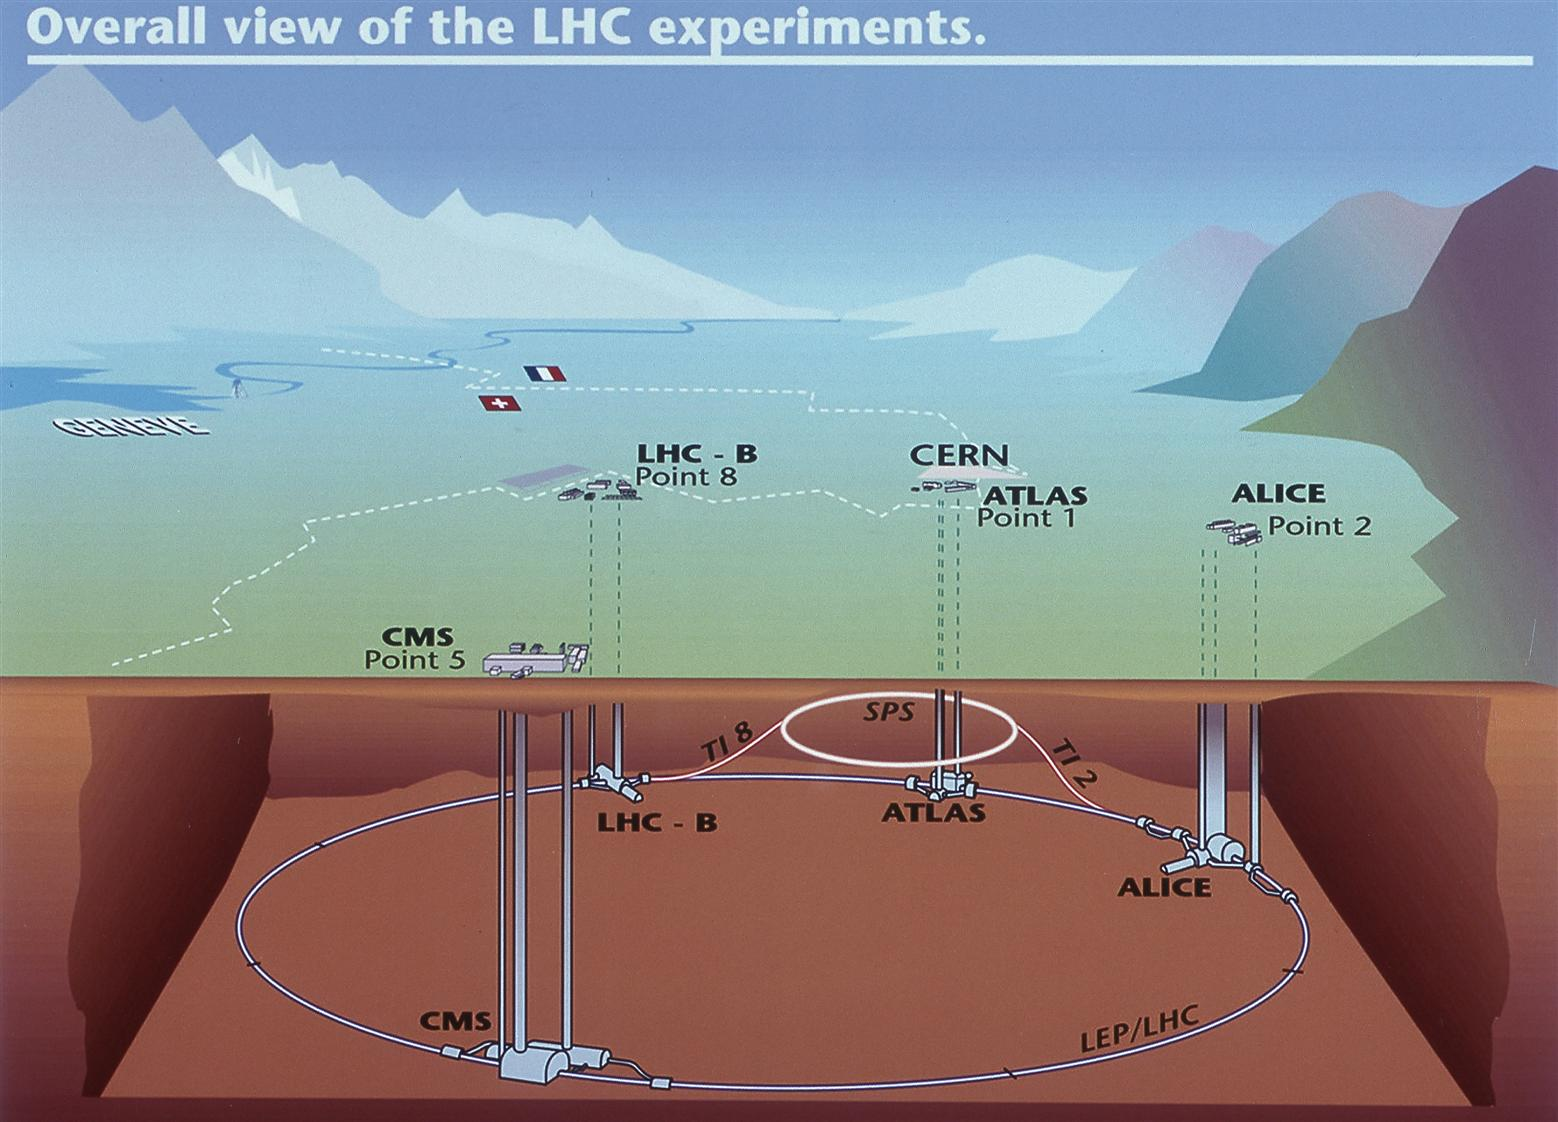
\includegraphics{figures/experiment/LHC_IPs}}
	\caption{The LHC and the four interaction points where the beams are brought into collision. The ATLAS experiment is located at interaction point 1.}
	\label{fig:LHC-IPs}
\end{figure}


The LHC project was approved in 1994 by the CERN Council, and construction proceeded over the ensuing 14 years~\cite{Evans:2010va}. The collider detectors were constructed in parallel, beginning with the excavation of two additional caverns at IP1 and IP5 for the ATLAS and CMS detectors (LHCb and ALICE occupied the existing caverns at IP2 and IP8, which previously housed the DELPHI and L3 LEP experiments). The first beam was circulated on 10 September 2008; however, on 19 September, the LHC sustained severe damage due to an incident stemming from a faulty joint between magnets\footnote{A postmortem analysis implicated a bad splice between the superconducting cables of adjacent magnets as the source of the incident, with a resistance about $10^3$ times above specification. The joint melted, and \SI{275}{\mega\joule} of energy in the magnets dissipated in electric arcs, which vaporized beam pipes and breached the cryogenic vessel containing the magnets. A large amount of liquid helium entered the vacuum vessel and heated rapidly, breaking several vacuum barriers of the cryostats with a force of up to 56 tons. Ultimately, 30 dipoles and 7 quadrupoles were damaged beyond repair, and another 9 dipoles and 7 quadrupoles required repairs; 9 magnet interconnections were destroyed; 26 magnets were pushed down the tunnel; \SI{276}{\mega\joule} of energy were dissipated in electrical faults and arcs; 6 tons of helium were lost; and \SI{2.8}{\kilo\meter} of both beam pipes were contaminated with fragments of insulation, with \SI{1}{\kilo\meter} also contaminated with soot from molten copper and insulation.~\cite{Rossi:2010el}}. Repairs took an extra year, and the energy of the beams was reduced to 3.5-\SI{4}{\tera\electronvolt} for the first data-taking run, to mitigate the risk of another possible faulty joint. 

Proton-proton collisions at a center-of-mass energy of $\sqrt{s}=\SI{7}{\tera\electronvolt}$ commenced in early 2010. The LHC delivered an integrated luminosity of $\int \mathcal{L}\, dt=\SI{48.1}{\pico\barn\tothe{-1}}$ to the ATLAS detector in 2010, and $\int \mathcal{L}\, dt=\SI{5.46}{\femto\barn\tothe{-1}}$ in 2011. In 2012, the collision energy was increased to $\sqrt{s}=\SI{8}{\tera\electronvolt}$, and a dataset of $\int \mathcal{L}\, dt=\SI{22.8}{\femto\barn\tothe{-1}}$ was delivered. 

\subsection{Accelerator Components}
The primary devices used for acceleration are synchrotrons, circular accelerators comprised of magnets and radio frequency (RF) cavities~\cite{wiedemann2007particle}. The magnets are used to manipulate the particle beams: dipole magnets bend the beams in a circle and steer the beams down transfer lines between the accelerators, while quadrupole and higher moment magnets focus the beams. RF cavities are hollow metallic structures used for particle acceleration. The RF cavities are driven by klystrons, radio frequency amplifiers that act as power sources, at their resonant frequency, creating an oscillating electric field inside the structure. The frequency of the RF cavities is matched to the rotation frequency of the particle beams.

The RF oscillations cause the particle beam to bunch longitudinally into so-called RF buckets, shown schematically in figure~\ref{fig:RF-bucket}. The center of the bucket corresponds to particles with the reference energy, determined by the magnets, which arrive in phase with the RF oscillations so that they experience no force. During \emph{flat-top} operation, where the particle are held at fixed energy in the synchrotron, particles at the center of the RF bucket remain stationary at that point (neglecting energy losses due to synchrotron radiation), while nearby particles oscillate around the fixed point. During a \emph{ramp}, where particles are accelerated, the magnetic fields of the dipoles are slowly increased, shifting the RF bucket and causing the particle bunches to fall on the accelerating edge of the electric field oscillations. 

\begin{figure}[htbp]
	\centering
	\resizebox{0.5\textwidth}{!}{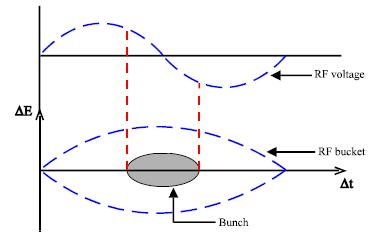
\includegraphics{figures/experiment/LHC_RF_buckets}}
	\caption{Schematic picture of an RF bucket.}
	\label{fig:RF-bucket}
\end{figure}

\FloatBarrier

\subsection{The Accelerator Complex}

\subsubsection{Injection Chain}

\begin{figure}[htbp]
	\centering
	\resizebox{3.5in}{!}{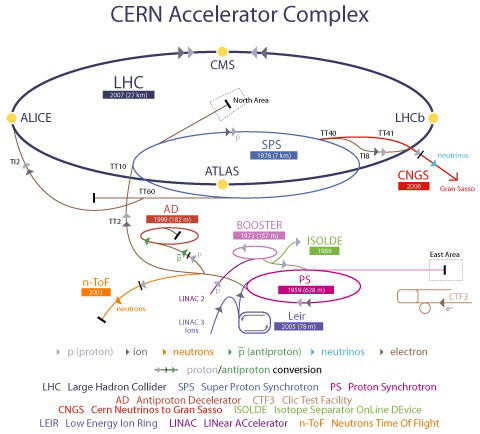
\includegraphics{figures/experiment/converted/LHC_accelerator_complex.png}}
	\caption{The LHC accelerator complex. The proton injection chain begins at LINAC2, proceeding through the booster, PS, and SPS before reaching the LHC. The facility also provides ions to the LHC, as well as a variety of particles to other experiments.}
	\label{fig:LHC-accelerator-complex}
\end{figure}


The LHC itself is the last stage of a chain of lower-energy accelerators, shown in figure~\ref{fig:LHC-accelerator-complex}~\cite{Benedikt:2004wm}. The staged acceleration chain preserves the high-quality of the beam over many decades of energy. It consists of a linear accelerator and three synchrotrons which were used for previous generations of experiments at CERN. The reuse of the older accelerators is economical while still meeting the stringent performance requirements of the LHC, providing up to 2808 proton bunches with a very small transverse emittance and controllable longitudinal emittance. 

Protons are produced from hydrogen gas using a duoplasmatron source, which strips electrons from protons in a high electric field. After passing through a $\SI{90}{\kilo\volt}$ pre-injector, a radio frequency quadrupole (RFQ) focuses and accelerates the protons to $\SI{750}{\kilo\volt}$. A linear accelerator (LINAC2) then accelerates the protons to $\SI{50}{\mega\electronvolt}$ using RF cavities. The protons then pass through an $\SI{80}{\meter}$-long transfer line into the the Proton Synchrotron Booster (PSB) and Proton Synchrotron (PS). 

The PSB consists of four stacked circular synchrotrons, $\SI{157}{\meter}$ in circumference, and accelerates the protons to $\SI{1.4}{\giga\electronvolt}$. The use of four separate rings mitigates the space charge effects caused by the repulsion of protons within a bunch, which scale as $N_b/(\beta\gamma^2)$, where $N_b$ is the number of protons per bunch. The protons are then injected into single-ring PS, where the higher injection energy reduces the space charge effect. The RF cavities of the PS, operating at several frequencies, accelerate the beams to $\SI{26}{\giga\electronvolt}$, and also split the protons into the bunches eventually inject into the LHC. Nominally, this yields 72 bunches separated by \SI{25}{\nano\second}, but for Run I, \SI{50}{\nano\second} spacing was used instead. 

The protons are extracted from the PS at intervals of \SI{3.6}{\second} and injected into the third synchrotron in the chain, the $\SI{7}{\kilo\meter}$-circumference Super Proton Synchrotron (SPS). Immediately prior to extraction, the bunches are rotated by increasing the RF voltage, reducing the longitudinal emittance in order to ease capture in the SPS RF buckets, which have a frequency of $\SI{200}{\mega\hertz}$.  Up to four PS batches are injected per SPS cycle, after which the particle are accelerated at an average of $\SI[per-mode=symbol]{78}{\giga\electronvolt\per\second}$ to the LHC injection energy of $\SI{450}{\giga\electronvolt}$. Flat-top is maintained for about one second, during which the injection is prepared:

\begin{itemize}
	\item The magnets used for the beam extraction are ramped, safety checks are performed, and the SPS phase is tuned to match that of the LHC.
	\item The bunch length is compressed using an RF voltage increase, as in the PS-SPS transfer.
	\item The tails of the bunches are removed, down to $3$--$3.5\sigma$.
\end{itemize}

The SPS cycle takes 21.6 seconds, leading to a total LHC filling time of about nine minutes.

\subsubsection{LHC Main Ring}
The LHC main ring accelerates protons from the injection energy of $\SI{450}{\giga\electronvolt}$ to the collision energy, which ranged from $\SI{3.5}{\tera\electronvolt}$ to $\SI{4}{\tera\electronvolt}$ for proton-proton collisions during Run I~\cite{Bruning:2004ej}. The \SI{26.7}{\kilo\meter} ring consists of eight arcs and eight straight sections, shown in figure~\ref{fig:LHC-segments}. Each straight section is called an \emph{insertion region} (IR), and contain either collider experiments or important services. IRs 1, 2, 5, and 8 contain the ATLAS, LHCb, CMS, and ALICE experiments, respectively; IR 4 contains two independent $\SI{400}{\mega\hertz}$ RF systems, one for each of the counter-rotating beams; IR 6 contains the beam dump system; and IRs 3 and 7 contain collimation systems. The beams are contained in separate beam pipes except at the collision points.

\begin{figure}[htbp]
	\centering
	\resizebox{0.5\textwidth}{!}{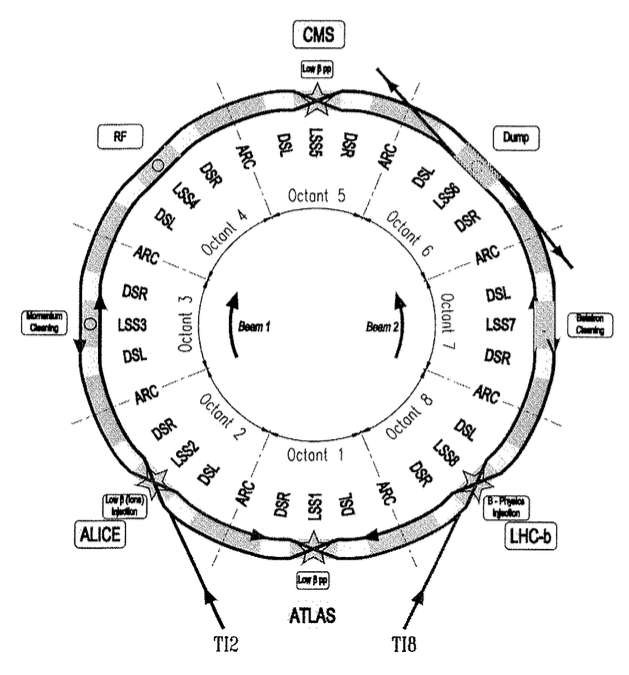
\includegraphics{figures/experiment/LHC_segments}}
	\caption{Layout of the LHC. The ring consists of eight arcs and eight long straight sections (LSS). Each junction between an arc and a LSS contains a dispersion suppressor cell (DSL, DSR). TI2 and TI8 are the two injection tunnels (``tunnel d'injection'') leading from the SPS to the LHC.}
	\label{fig:LHC-segments}
\end{figure}


The beams are controlled by over 7,000 magnets. The primary bending and focusing are performed by 1232 superconducting dipole and 392 superconducting quadrupole magnets. The dipole magnets, shown in figure~\ref{fig:LHC-dipole-magnets}, have a nominal maximum field of $\SI{8.33}{\tesla}$ and a length of $\SI{15}{\meter}$. The conducting coils are constructed from Nb-Ti Rutherford cables, and are cooled to $\SI{1.9}{\kelvin}$ using superfluid helium. The dipoles have a double-bore structure, so that a single magnet provides the bending field for both beams. 

\begin{figure}[htbp]
	\centering
	\subfloat[] {
		\resizebox{0.45\textwidth}{!}{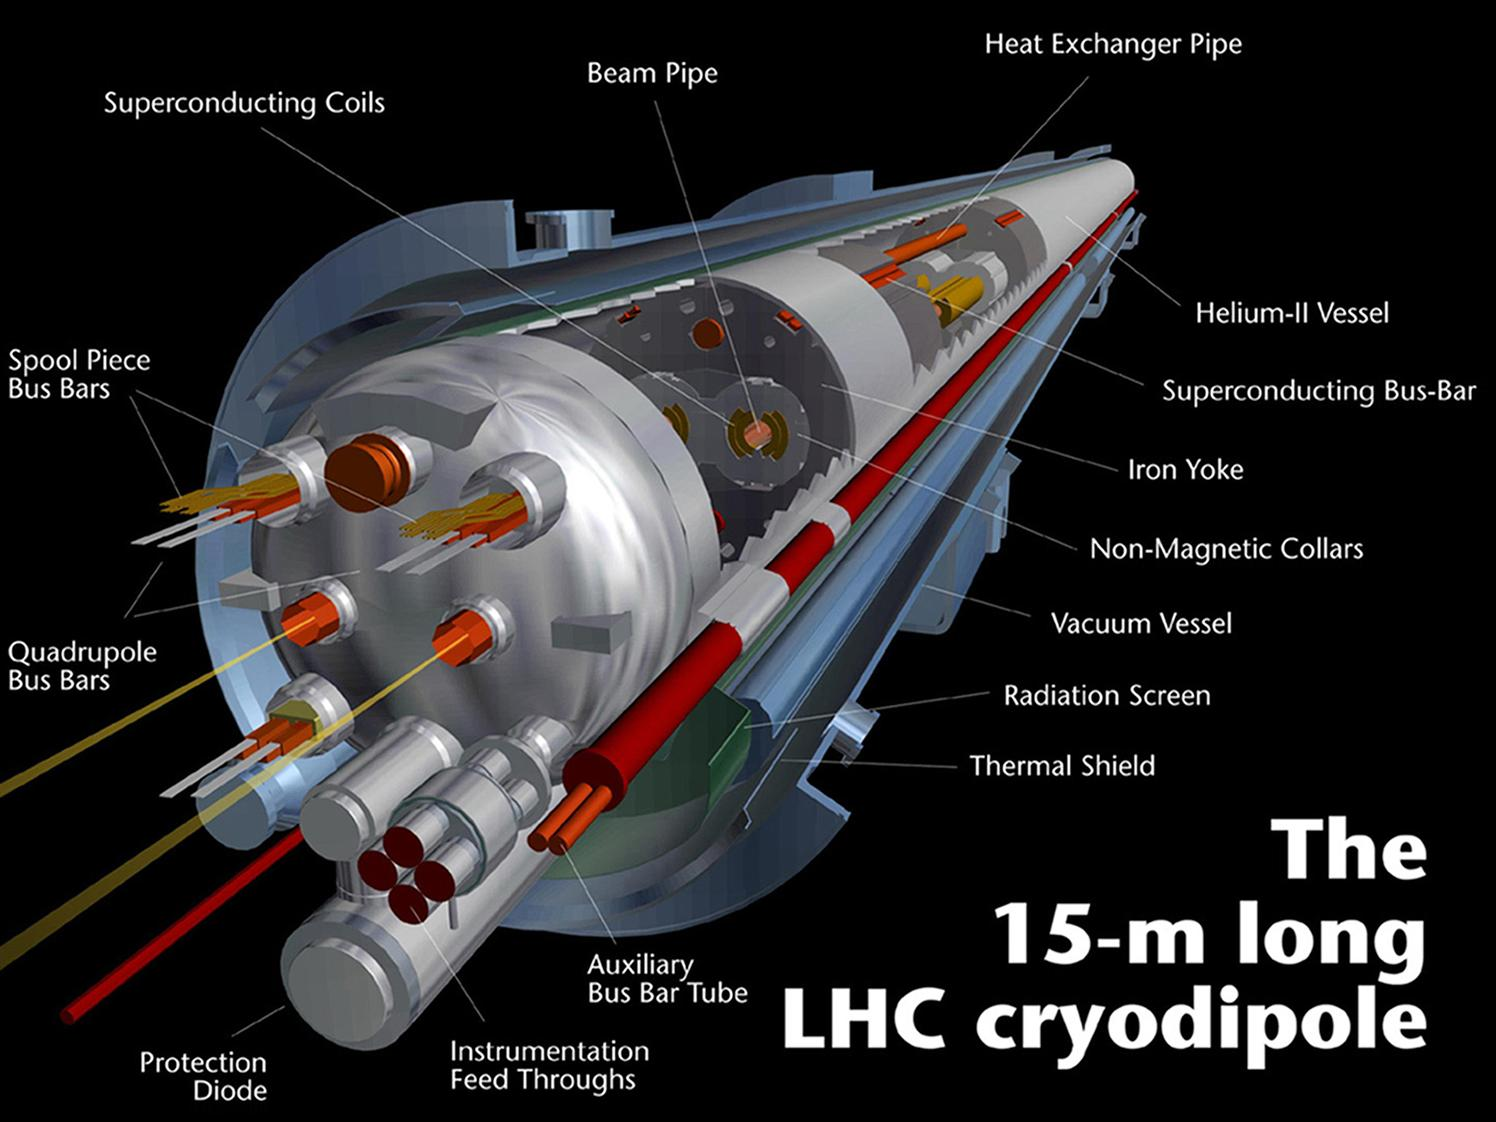
\includegraphics{figures/experiment/LHC_dipole_sketch}}
	}
	\hfill
	\subfloat[] {
		\resizebox{0.45\textwidth}{!}{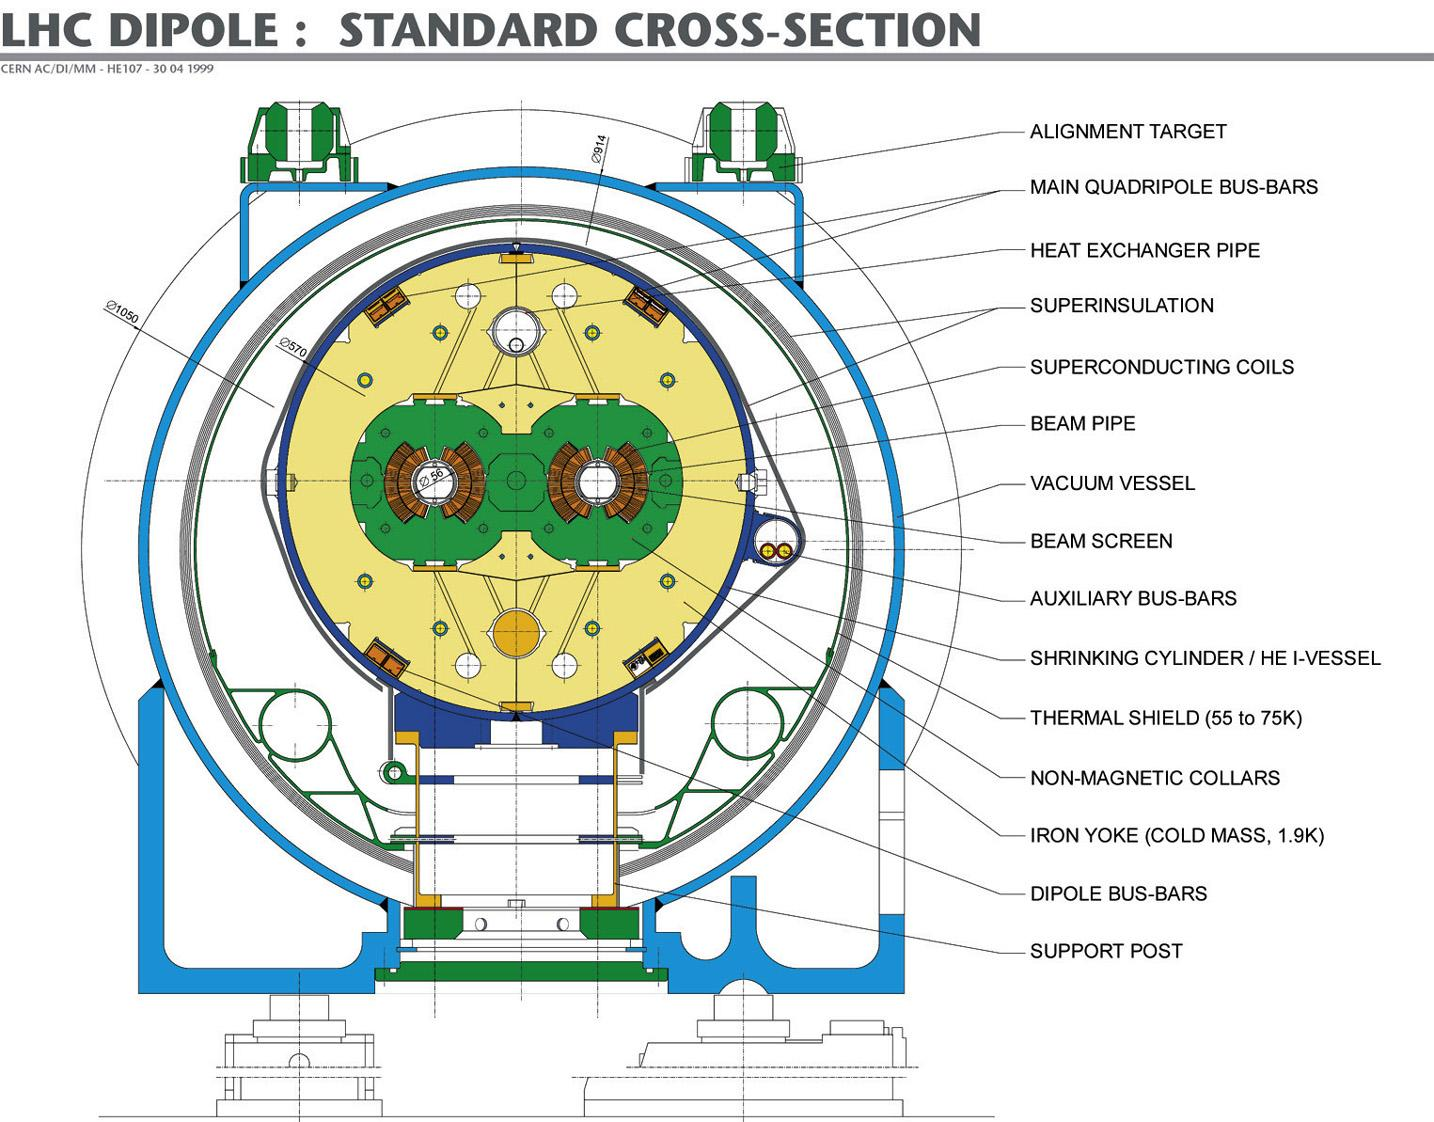
\includegraphics{figures/experiment/LHC_dipole_xsec}}
	}
	\caption{Two views of the LHC superconducting dipole magnet. The magnets are $\SI{15}{\meter}$ long and have two bores, one for each of the counter-rotating beams.}
	\label{fig:LHC-dipole-magnets}
\end{figure}

The acceleration is provided by two superconducting RF systems, one for each beam. The RF cavities are constructed from copper with a thin (\SIrange{1}{2}{\micro\meter}) layer of niobium, and operate at $\SI{4.5}{\kelvin}$. The single-cell cavities, each nominally providing $\SI{2}{\mega\volt}$, are arranged into cryomodules containing eight cells, for a total peak voltage of $\SI{16}{\mega\volt}$. A module consisting of two cells is shown in figure~\ref{fig:RF-module}. The RF frequency is $\SI{400}{\mega\hertz}$, giving an RF bucket length of $\SI{2.5}{\nano\second}$, or $\SI{75}{\centi\meter}$. 

\begin{figure}[htbp]
	\centering
	\subfloat[ A prototype cryomodule containing two cavities.] {
		\resizebox{0.45\textwidth}{!}{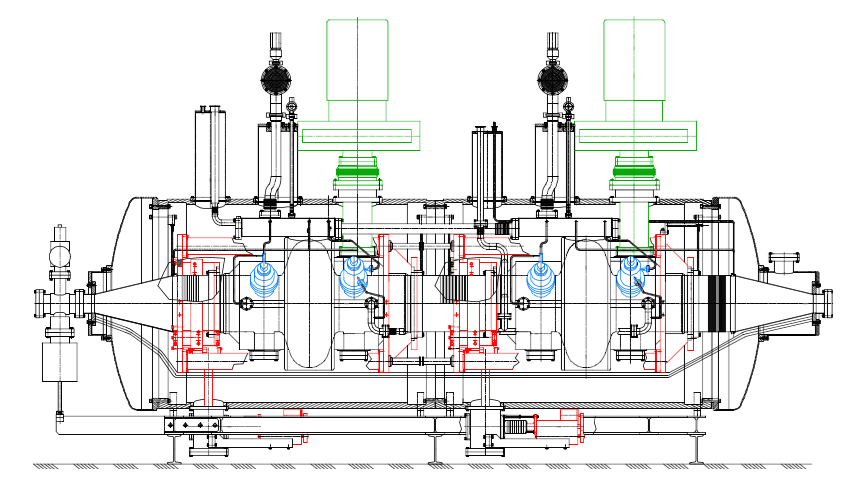
\includegraphics{figures/experiment/LHC_RF_cryomodule}}
	}
	\hfill
	\subfloat[ The RF cryomodules installed at IR4.] {
		\resizebox{0.45\textwidth}{!}{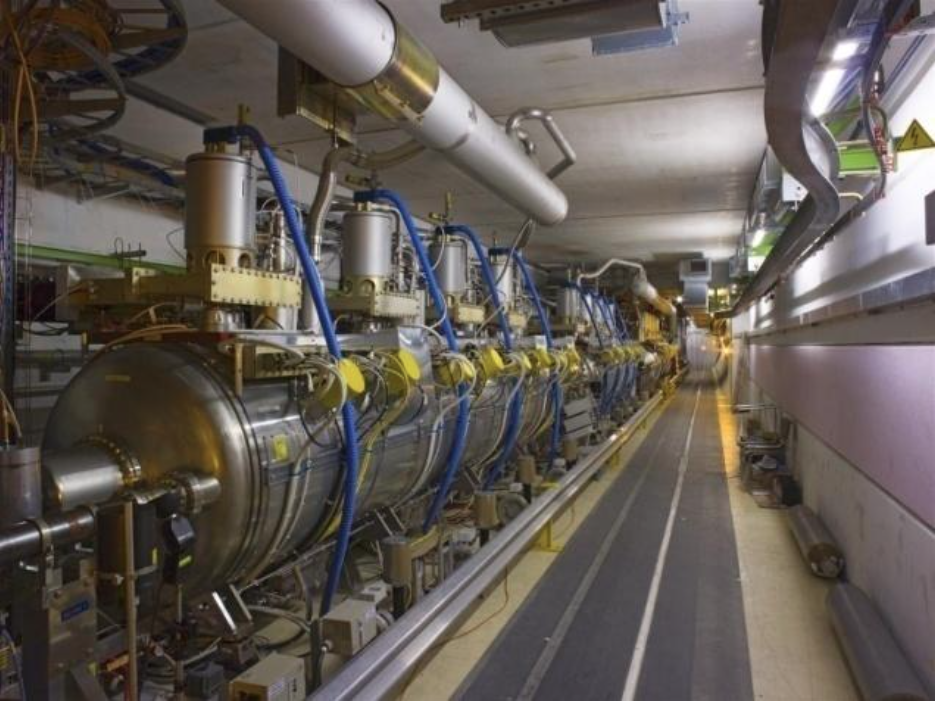
\includegraphics{figures/experiment/LHC_RF_IR4}}
	}
	\caption{The LHC RF cryomodules.}
	\label{fig:RF-module}
\end{figure}

At the collision points, the two beams converge in a single pipe for approximately $\SI{130}{\meter}$. A steering dipole directs the beams into collision, and a triplet of quadrupoles on each side of the interaction region focus the beam onto the interaction point, squeezing the beams in the transverse directions from a typical orbiting width of $\mathcal{O}(\SI{1}{\milli\meter})$ to a collision width of $\mathcal{O}(\SI{10}{\micro\meter})$. 


\subsection{Beam Parameters}
From the experiments' point of view, there are two main parameters to optimize in order to maximize sensitivity to new physics: the collision energy, $\sqrt{s}$, and the integrated luminosity, $L=\int \mathcal{L}\, dt$. The collision energy is limited to $\sqrt{s}=\SI{14}{\tera\electronvolt}$ by the bending power of the dipole magnets, which have a nominal field strength of $\SI{8.33}{\tesla}$; however, due to the faulty splice design mentioned above, the energy was limited to $\sqrt{s}=7$--$\SI{8}{\tera\electronvolt}$ in Run I. 

The optimization of the integrated luminosity is somewhat more complicated. The instantaneous luminosity of two colliding bunches is given by:
\begin{equation}\label{eqn:lumi}
	\mathcal{L} = \frac{f_r N_1 N_2 \gamma_b}{4\pi \epsilon_n \beta_{*}} F(\alpha),
\end{equation}
where $f_r=\SI{11245.5}{\hertz}$ is the LHC revolution frequency, $N_{1,2}$ are the numbers of protons in the two beams, $\gamma_b$ is the relativistic gamma factor, $\epsilon_n$ is the normalized transverse emittance, $\beta_{*}$ is the beta function at the collision point, and $F(\alpha)$ is the reduction in luminosity due to a nonzero beam crossing half-angle of $\alpha$. The total instantaneous luminosity is given by the sum of all colliding bunch pairs. 

% TO DO: beta* formula?

In general, a higher total integrated luminosity is desired. This depends on a number of factors:

\begin{itemize}
	\item The instantaneous luminosity per bunch, $\mathcal{L}=\frac{f_r N_1 N_2}{4\pi\epsilon_n \beta_{*}}$. A higher $\mathcal{L}$ increases the number of simultaneous collisions per bunch crossing (\emph{pileup}), $\mu=L_b/\sigma_{\mathrm{inel}}$, which degrades the performance of the detectors. 
	% Removed for now. According to Frank Zimmerman's slides, no beam-beam limit was found in MDs! 
	% From the accelerator's point of view, the number of protons per bunch, $N_{1,2}$, and the transverse emittance are limited by non-linear beam-beam effects~\cite{Papotti:2014vb}. Typical values during 2012 were $N_{1,2}=1.65\times 10^{11}$ and $\epsilon_n=2.5~\micron$, giving pileup values at the start of a fill of around 30, with tails up to $\sim$40. 

	\item The number of bunches in the LHC, $n_b$. During Run I, the LHC was filled with 1380 bunches with $\SI{50}{\nano\second}$ spacing between bunches, as opposed to the nominal 2808 bunches with $\SI{25}{\nano\second}$ spacing. The advantages of $\SI{50}{\nano\second}$ spacing include less days needed for electron-cloud scrubbing, smaller transverse emittances, and a smaller crossing angle~\cite{Papotti:2014vb}. The primary disadvantage is a higher pileup for the experiments. 

	\item The crossing angle, $\alpha$. A nonzero crossing angle is required to prevent \emph{parasitic collisions} between bunches away from the nominal collision point. For bunches spaced by $\SI{25}{\nano\second}$, there are 34 unwanted parasitic collision points inside the common beam pipe at each interaction region. The reduction in luminosity is:

	\begin{equation}
		F(\alpha)=\frac{1}{\sqrt{1+\left(\frac{2\alpha \sigma_z}{2\sigma^*}\right)}},
	\end{equation}
	
	where $\sigma_z$ is the RMS bunch length and $\sigma^{*}$ is the transverse beam width at the collision point. During normal 2012 running conditions, the crossing half-angle was $\alpha=\SI{145}{\micro\radian}$, and the luminosity reduction factor was about $18\%$. 

	\item The fill schedule of the LHC. The instantaneous luminosity of the LHC decreases over time. The dominant loss of luminosity is due to the loss of protons from the collisions themselves, with a typical decay constant of $\tau_{\mathrm{nuclear},1/e}=\SI{29}{\hour}$. Including other sources of loss such as intra-bunch scattering, scattering from collisions with gas in the beam pipe, beam-beam effects, and RF noise, the typical luminosity lifetime is $\tau_L=\SI{14.9}{\hour}$. 

	The the fill schedule can be optimized to maximize the luminosity based on $\tau_L$ and the average turnaround time to refill the LHC after a beam dump, $T_{\mathrm{turnaround}}$. This can be quantified using the \emph{H{\"u}bner factor}, $\mathrm{HF}_{\mathrm{peak}}$, defined as the ratio of the delivered integrated luminosity to the hypothetical integrated luminosity with $\tau_L=\infty$ and $T_{\mathrm{turnaround}}=0$. In 2011, this was typically in the range $15\%$--$20\%$.
\end{itemize}

The delivered luminosity in 2011 and 2012 will be discussed later in chapter~\ref{ch:luminosity}.


\section{The ATLAS Experiment}\label{sec:the-atlas-experiment}

The ATLAS detector~\cite{TheATLASCollaboration:2008fg} is a large, cylindrical collider detector located at IR1 on the LHC ring (figure~\ref{fig:LHC-IPs}). The detector measures the energy and momenta of particles produced in the collisions provided by the LHC. It consists of several subsystems occupying a cylinder with a diameter of $\SI{25}{\meter}$ and a length of $\SI{46}{\meter}$, with a combined weight of approximately 7,000~tons. Closest to the interaction region, the inner detector measures the momenta of charged particles by tracking their movement through a solenoidal magnetic field. Outside the inner detector solenoid magnet, electromagnetic and hadronic calorimeters measure the energy of electrons, photons, and hadrons. Finally, the muon spectrometer provides additional tracking and particle identification for muons in large toroidal magnetic field. 

This section describes the design of the magnets, inner detector, calorimeters, and muon spectrometer. The reconstruction of physics objects from the detector measurements is described in chapter~\ref{ch:event-reconstruction}. 

\subsection{Coordinate System}\label{sec:ATLAS-coordinate-system}

The ATLAS detector uses a right-handed coordinate system, with $\hat{x}$ pointing from the interaction point towards the center of the LHC ring, $\hat{y}$ pointing up, and $\hat{z}$ pointing along the ring towards IR2. Due to the symmetry of the detector, cylindrical coordinates ($r,\theta,\phi$) are often used, with $r$ the transverse distance from the beam line, $\theta$ the polar angle from the beamline, and $\phi$ the azimuthal angle in the $x$-$y$ plane. The polar angle can also be expressed in term of the pseudorapidity, $\eta = -\log \tan \frac{\theta}{2}$, which is useful for describing the geometry of particles in part because differences in pseudorapidity, $\Delta\eta$, are invariant under longitudinal Lorentz boosts along $\hat{z}$. For massless particles, the pseudorapidity is equal to the rapidity, $y=\frac12 \log \frac{E+p_z}{E-p_z}$. 

\subsection{Magnets}\label{sec:ATLAS-magnets}
ATLAS relies on four powerful superconducting magnets to bend the trajectories of charged particles, allowing the tracking detectors to provide measurements of their momenta. The solenoid provides a $\SI{2}{\tesla}$ axial magnetic field in the volume of the inner detector, while the barrel and two endcap toroids provide a toroidal magnetic field ranging from $0.5$--$\SI{1}{\tesla}$ for the muon spectrometer. The geometry of the magnets is shown in figure~\ref{fig:ATLAS-magnets-sketch}. Key parameters for the magnet system are shown in table~\ref{table:ATLAS-magnet-parameters}.

\begin{figure}[htbp]
	\centering
	\resizebox{0.6\textwidth}{!}{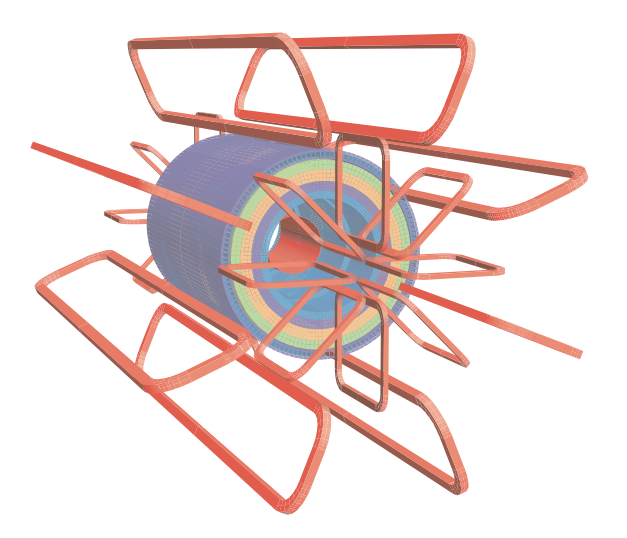
\includegraphics{figures/experiment/ATLAS_magnets_sketch}}
	\caption{The geometry of the magnet windings and tile calorimeter steel. The three toroids and solenoid are shown in red. The remaining colors show layers of the tile calorimeter with different magnetic properties and an outside return yoke~\cite{atlasphotos}.}
	\label{fig:ATLAS-magnets-sketch}
\end{figure}


\begin{table}[htbp]
	\centering
	\scriptsize
	\begin{tabular}{|l|l|c|c|c|c|}
		\hline
		\textbf{Property} & \textbf{Feature} & \textbf{Unit} & \textbf{Solenoid} & \textbf{Barrel toroid} & \textbf{End-cap toroids} \\
		\hline
		\textbf{Size} & Inner diameter & m & $2.46$ & $9.4$ & $1.65$ \\
		\hline
		 & Outer diameter & m & $2.56$ & $20.1$ & $10.7$ \\
		\hline
		 & Axial length & m & $5.8$ & $25.3$ & $5.0$ \\
		\hline
		 & Number of coils & & $1$ & $8$ & $2\times 8$ \\
		\hline
		\textbf{Mass} & Conductor & t & $3.8$ & $118$ & $2\times 20.5$ \\
		\hline
		 & Cold mass & t & $5.4$ & $370$ & $2\times 140$ \\
		\hline
		 & Total assembly & t & $5.7$ & $830$ & $2\times 239$ \\
		\hline
		\textbf{Coils} & Turns per coil & & $1154$ & $120$ & $116$ \\
		\hline
		 & Nominal current & kA & $7.73$ & $20.5$ & $20.5$ \\
		\hline
		 & Magnet stored energy & GJ & $0.04$ & $1.08$ & $2\times 0.25$ \\
		\hline
		 & Peak field in the windings & T & $2.6$ & $3.9$ & $4.1$ \\
		\hline
		 & Field range in the bore & T & $0.9$-$2.0$ & $0.2$-$2.5$ & $0.2$-$3.5$ \\
		\hline
	\end{tabular}
	\caption{Main parameters of the ATLAS magnet system~\cite{TheATLASCollaboration:2008fg}.}
	\label{table:ATLAS-magnet-parameters}
\end{table}




\subsubsection{Solenoid}\label{sec:ATLAS-magnets-solenoid}

The central solenoid, shown in figure~\ref{fig:solenoid}, occupies the volume between the inner detector and the electromagnetic calorimeter, with an inner radius of $\SI{2.46}{\meter}$, an outer radius of $\SI{2.56}{\meter}$, and a length of $\SI{5.8}{\meter}$. The single coil has 1154 windings made of high strength Al-stabilized NbTi conductor. With a nominal current of $\SI{7.73}{\kilo\ampere}$, the magnetic field is $\SI{1.998}{\tesla}$ at the center of the solenoid, falling to $\SI{1.8}{\tesla}$ at $z=\SI{1.7}{\meter}$ and $\SI{0.9}{\tesla}$ the end of the inner detector cavity.  The magnetic flux is returned via the steel in the hadronic calorimeter and its support structures. Liquid helium is used to cool the superconducting coil to an operating temperature of $\SI{4.5}{\kelvin}$. At nominal current, the stored energy is $\SI{40}{\mega\joule}$. 

The longitudinal and radial magnetic field components are shown for different $R$ and $z$ values in figure~\ref{fig:ATLAS-solenoid-Bfield}.

\begin{figure}[htbp]
	\centering
	\resizebox{0.6\textwidth}{!}{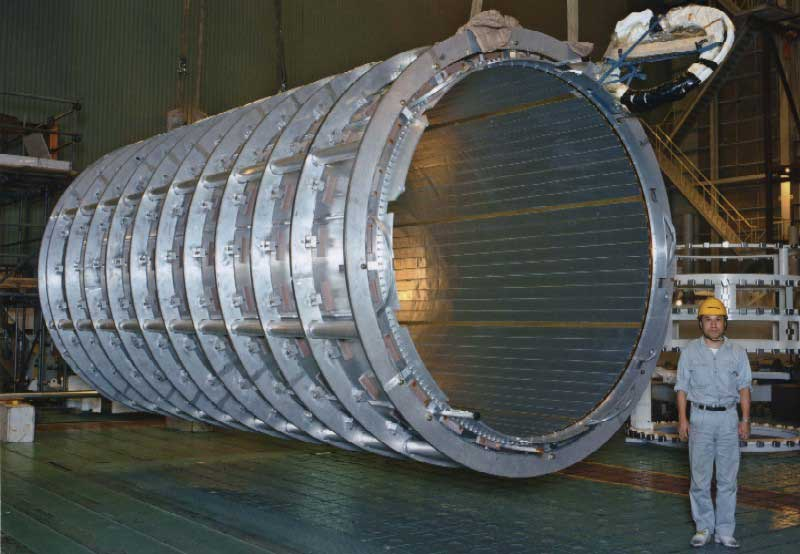
\includegraphics{figures/experiment/ATLAS_solenoid_2}}
	\caption{The central solenoid in the factory after completion of the coil winding~\cite{atlas-photos}.}
	\label{fig:solenoid}
\end{figure}

\begin{figure}[htbp]
	\centering
	\subfloat[] {\label{fig:ATLAS-solenoid-Bfield}
		\resizebox{0.4\textwidth}{!}{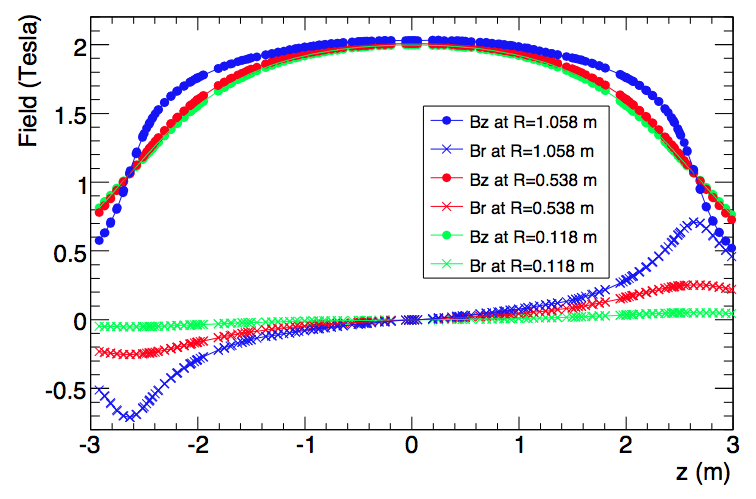
\includegraphics{figures/experiment/ATLAS_solenoid_Bfield}}
	}
	\hfill
	\subfloat[] {\label{fig:ATLAS-toroid-Bintegral}
		\resizebox{0.4\textwidth}{!}{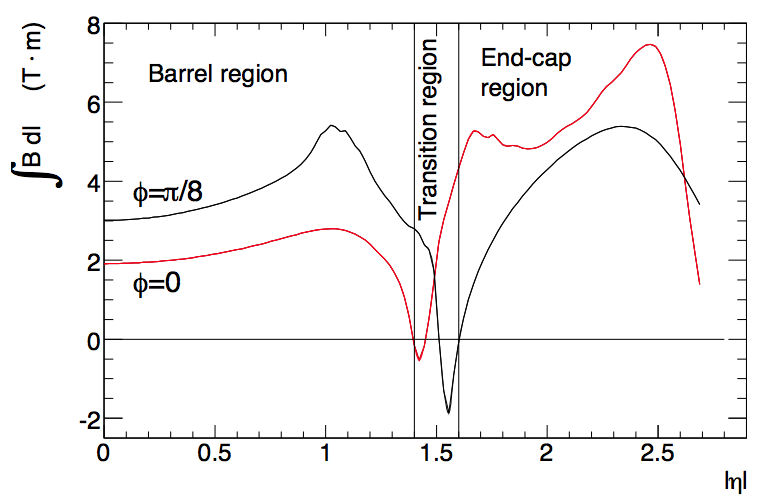
\includegraphics{figures/experiment/ATLAS_toroid_Bintegral}}
	}
	\caption{Left: the solenoid magnetic field in the radial ($B_r$) and longitudinal ($B_z$) directions, shown as a function of $z$ for $\phi=20\pi/16$ at different values of $R$. The field determined from a fit of the field model to measurements using an array of Hall probes~\cite{Aleksa:2008br}. Right: The predicted toroid magnetic field integral as a function of $|\eta|$. The integral is taken over a straight line through the interaction point, from the innermost to the outermost muon detector (section~\ref{sec:ATLAS-muon-spectrometer}).}
	\label{fig:ATLAS-magnets-Bfield}
\end{figure}


\subsubsection{Toroid}\label{sec:ATLAS-magnets-toroid}

The magnetic field for the muon spectrometer is provided by three large toroid magnets, each with eight superconducting coils. The magnets are shown in figure~\ref{fig:ATLAS-toroids}. The barrel toroid measures $\SI{25.3}{\meter}$ in length, with inner and outer diameters of $\SI{9.4}{\meter}$ and $\SI{20.1}{\meter}$, respectively. The two end-cap toroids are $\SI{5.0}{\meter}$ in length, with inner and outer diameters of $\SI{1.65}{\meter}$ and $\SI{10.7}{\meter}$, respectively. Both types of toroid contain eight coils, with 120 windings per coil in the barrel and 116 windings per coil in the end-caps. The end-cap coils are rotated by $\SI{22.5}{\degree}$ from the barrel coils to optimize the bending power in the overlap region between the magnets. Like the solenoid, the conductor is Al-stabilized NbTi, operated at $\SI{4.5}{\kelvin}$. The nominal current is $\SI{20.5}{\kilo\ampere}$, producing a magnetic field that varies from $\SI{0.15}{\tesla}$ to $\SI{2.5}{\tesla}$ in the barrel region, and $\SI{0.2}{\tesla}$ to $\SI{3.5}{\tesla}$ in the end-caps. The total stored energy at nominal current is $\SI{1.58}{\giga\joule}$. 

The field integral of the toroid is shown as a function of $\eta$ in figure~\ref{fig:ATLAS-toroid-Bintegral}. The field integral drops at the boundary between the barrel and end-caps, where the fields from the two magnets partially cancel. 

\begin{figure}[htbp]
	\centering
	\subfloat[ Barrel toroid.] {
		\resizebox{0.45\textwidth}{!}{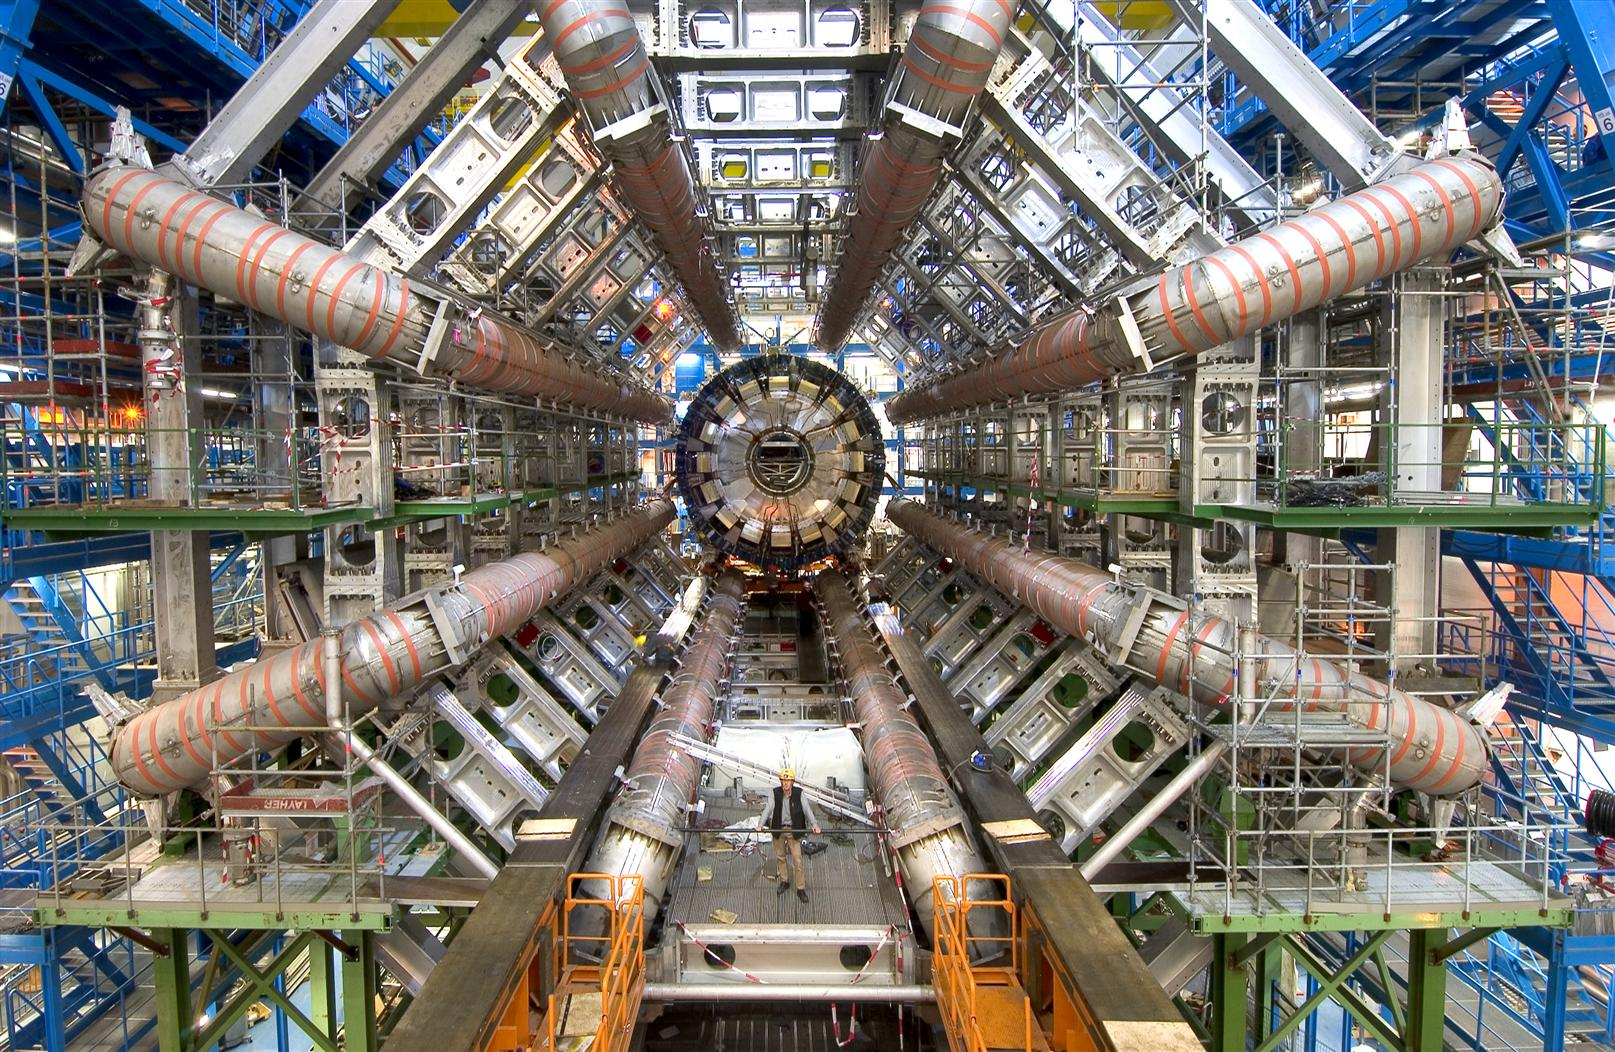
\includegraphics{figures/experiment/ATLAS_toroid}}
	}
	\hfill
	\subfloat[ End-cap toroid, inserted into the barrel toroid.] {
		\resizebox{0.45\textwidth}{!}{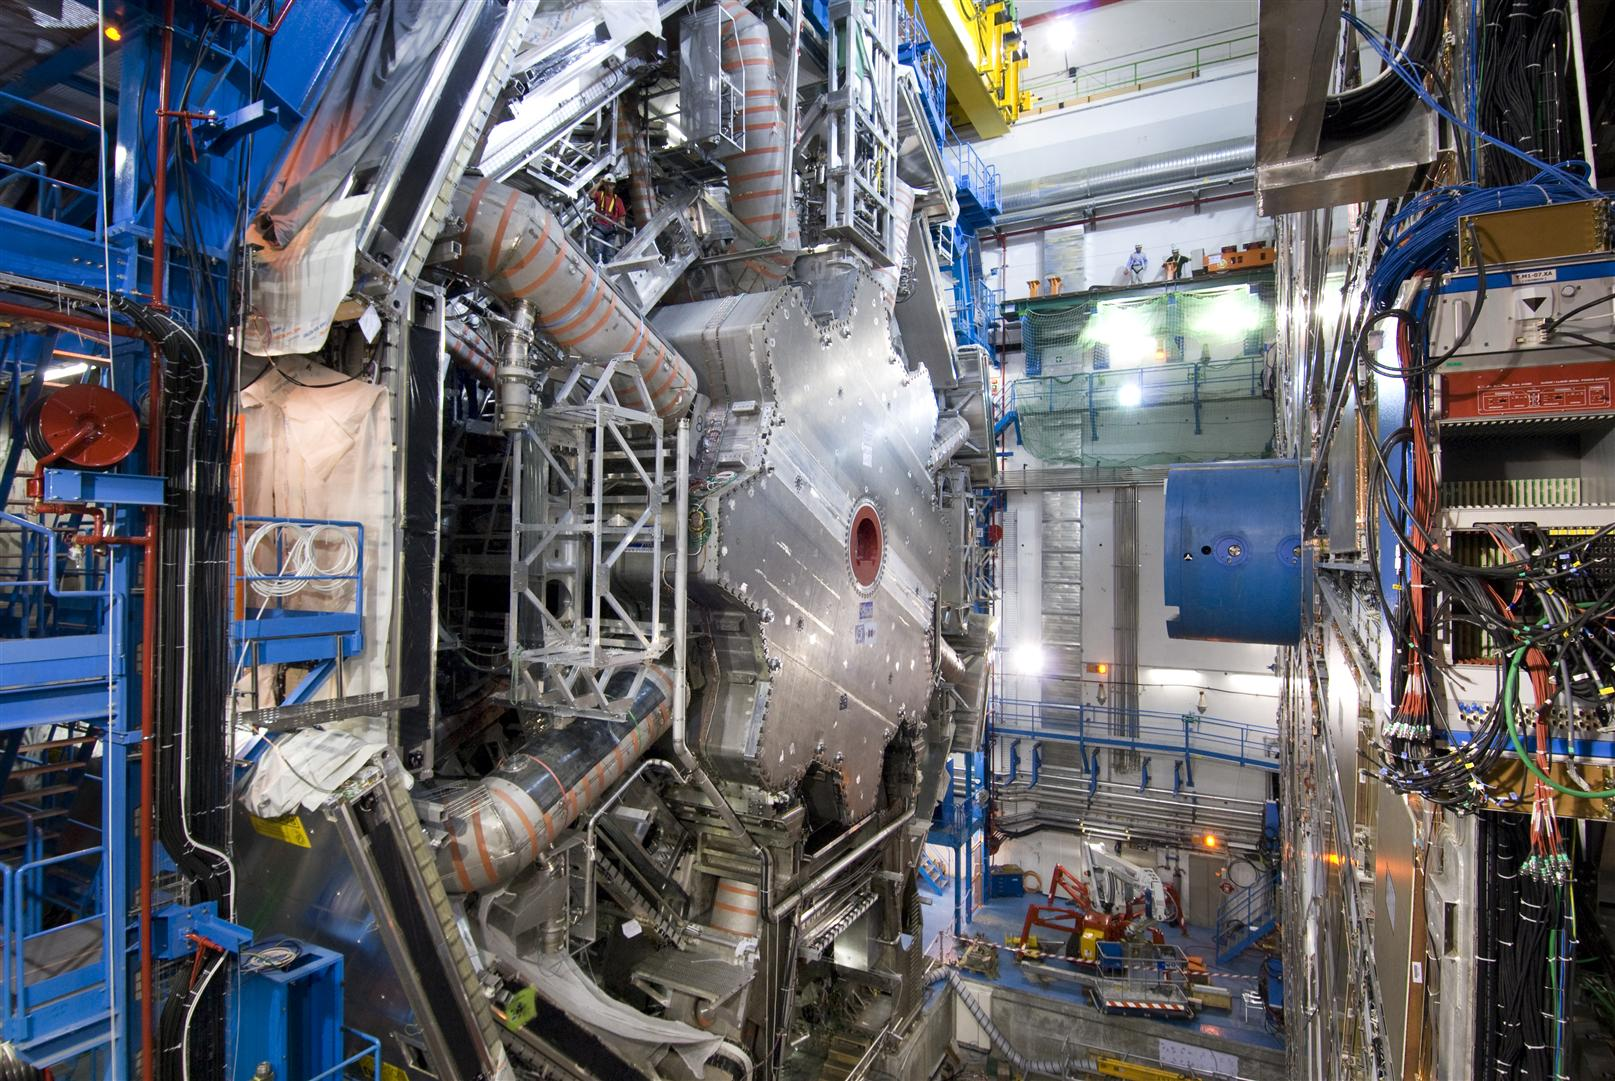
\includegraphics{figures/experiment/ATLAS_toroid_endcap_inserted2}}
	}
	\caption{Images of the barrel and end-cap toroid magnets during installation.}
	\label{fig:ATLAS-toroids}
\end{figure}




\subsection{Inner Detector}\label{sec:ATLAS-inner-detector}

The inner detector performs tracking of charged particles traversing the $\SI{2}{\tesla}$ solenoidal magnetic field in the pseudorapidity range $|\eta|<2.5$. It also performs electron identification in the range $|\eta|<2.0$. It consists of three subdetectors occupying the volume closest to the interaction region, directly outside the beam pipe, as shown in figure~\ref{fig:ATLAS-ID}. Proceeding outwards from the interaction point, these are the pixel detector, the semiconductor tracker (SCT), and the transition radiation tracker (TRT). The pixel detector provides three track measurements with high spatial resolution using silicon pixels. The SCT provides an additional four measurements using silicon strips. Finally, for particles with $|\eta|<2.0$, the TRT provides an average of 36 measurements per track using gas-filled straw tubes, which aids the pattern recognition, improves the momentum resolution, and performs electron identification. Examples of trajectories of $\SI{10}{\giga\electronvolt}$ particles through the barrel and end-cap layers are shown in figure~\ref{fig:ATLAS-ID-tracks}.

\begin{figure}[htbp]
	\centering
	\subfloat[ 3D model of the inner detector, showing the arrangement of the pixel detector, SCT, and TRT in the barrel and end-caps.] {
		\resizebox{0.45\textwidth}{!}{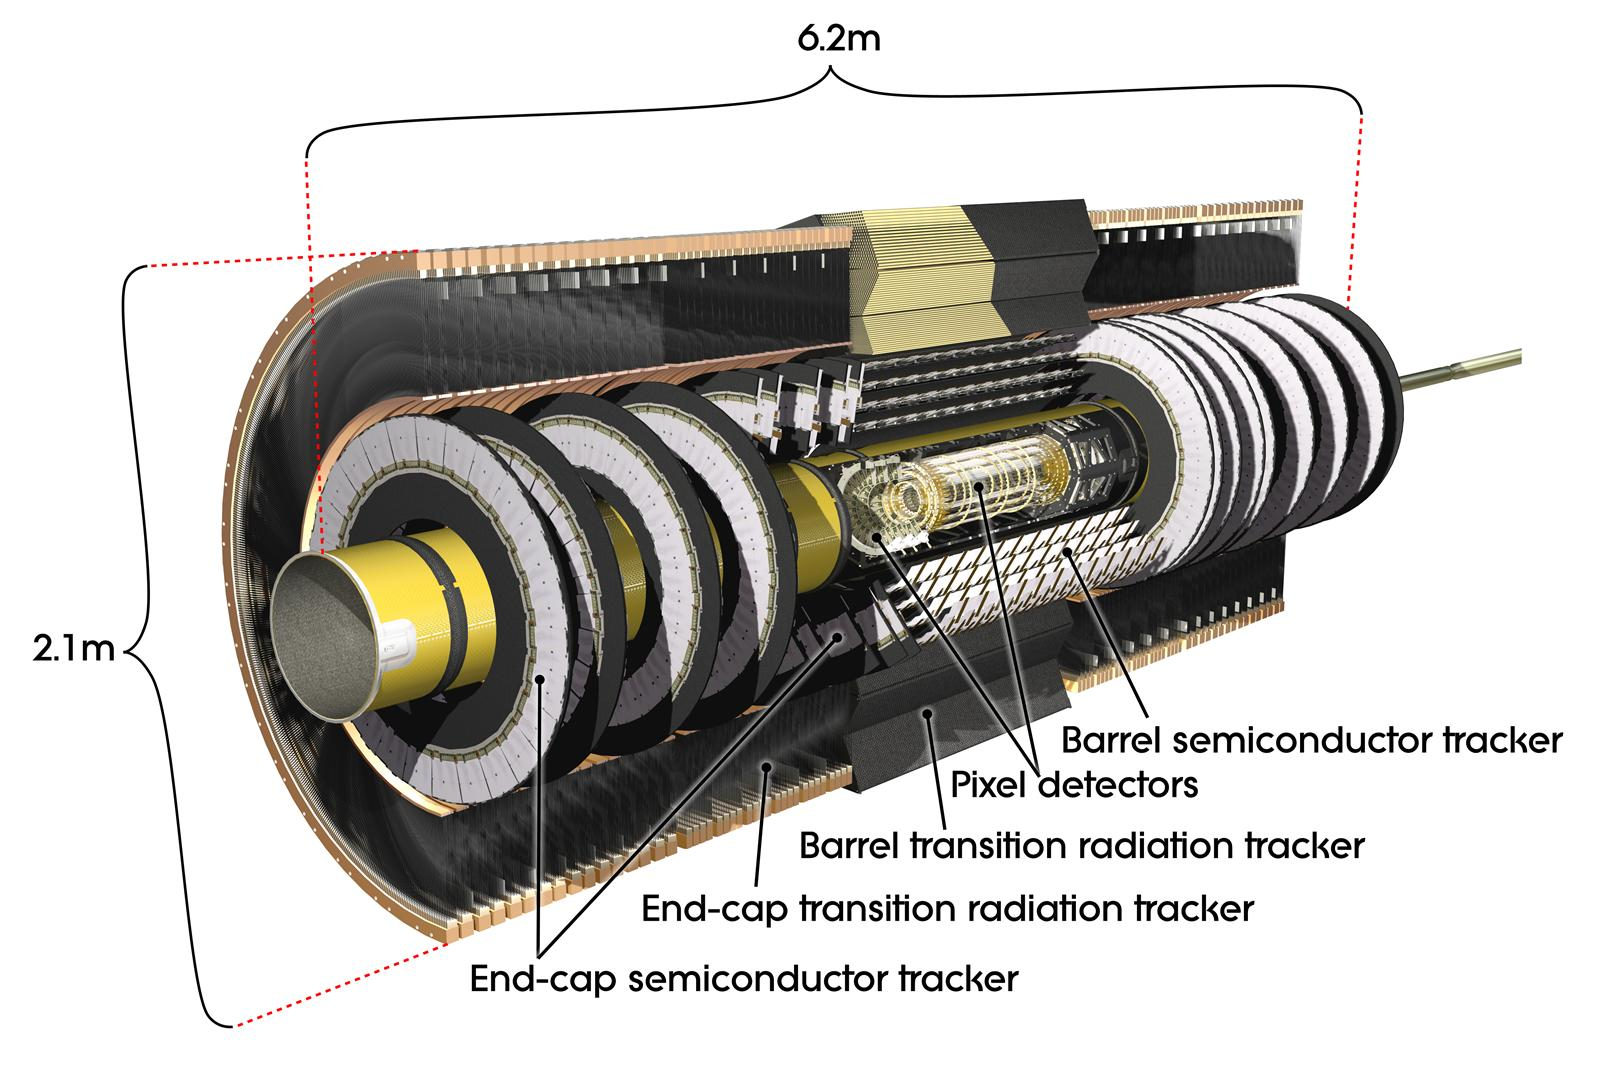
\includegraphics{figures/experiment/ATLAS_ID_sketch}}
	}
	\hfill
	\subfloat[ Layout of the inner detector in the $R-z$ plane.] {
		\resizebox{0.45\textwidth}{!}{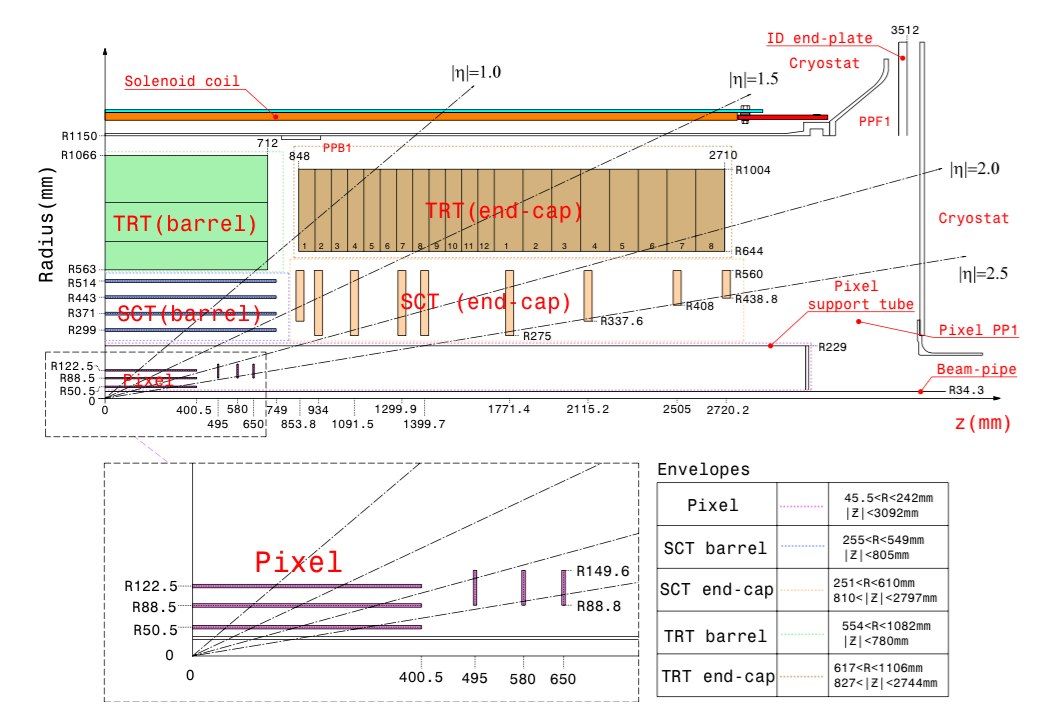
\includegraphics{figures/experiment/ATLAS_ID_layout_rz}}
	}
	\caption{Layout of the ATLAS inner detector.}
	\label{fig:ATLAS-ID}
\end{figure}

\begin{figure}[htbp]
	\centering
	\subfloat[ Trajectory of a $10 \GeV$ charged particle with $\eta=0.3$ traversing the barrel elements of the inner detector.] {
		\resizebox{0.4\textwidth}{!}{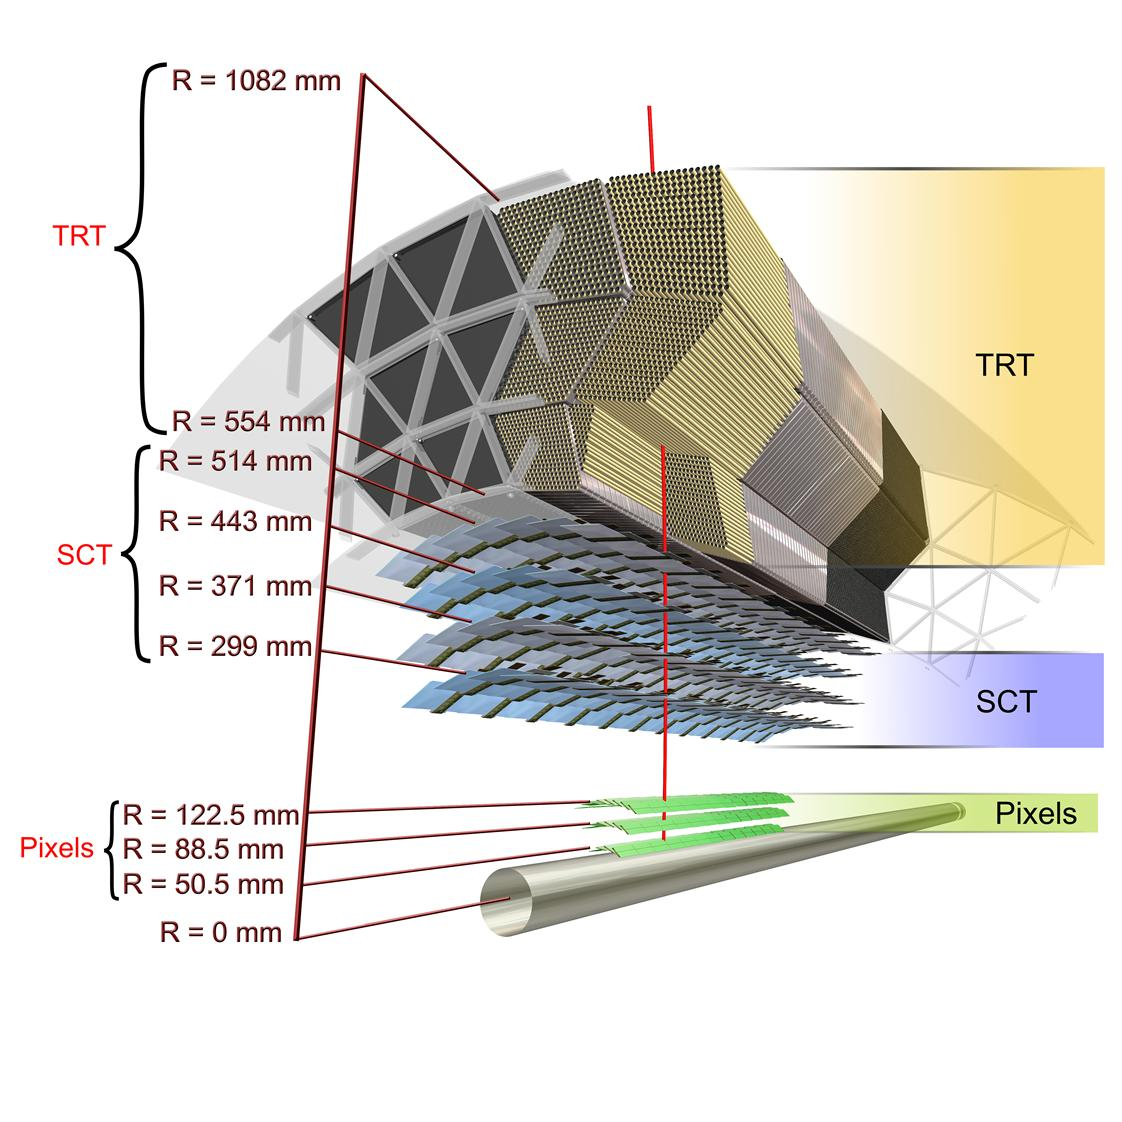
\includegraphics{figures/experiment/ATLAS_ID_track_barrel}}
	}
	\hfill
	\subfloat[ Trajectories of $10 \GeV$ charged particles with $\eta=1.4$ and $\eta=2.2$ traversing the barrel and end-cap elements of the inner detector.] {
		\vspace{-0.4in}
		\resizebox{0.55\textwidth}{!}{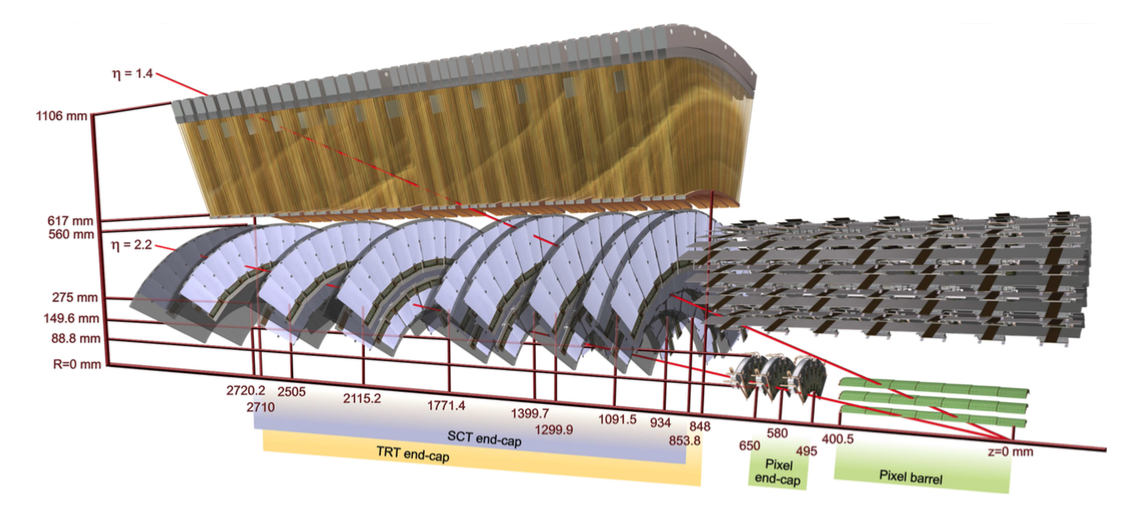
\includegraphics{figures/experiment/ATLAS_ID_track_endcap}}
	}
	\caption{Drawings of the inner detector sensors and structural elements traversed by $10 \GeV$ charged particles originating from the interaction point at various angles.}
	\label{fig:ATLAS-ID-tracks}
\end{figure}


\subsubsection{Pixel Detector}\label{sec:ATLAS-id-pixel-detector}

The pixel detector consists of 1744 identical pixel sensors, each measuring $19\times\SI{63}{\milli\meter\tothe{2}}$ and containing $144\times 328=47232$ pixels, for a total of $80.4\times 10^6$ pixels. The size of the pixels is dictated by the front-end electronics: in 128 of the 144 columns, the pixels have a pitch of $50\times \SI{400}{\micro\meter\tothe{2}}$, while the remaining 16 columns have a pitch of $50\times \SI{600}{\micro\meter\tothe{2}}$. For space reasons, eight pairs of pixels in each column are ganged to a common readout, giving a total of 46080 readout channels per sensor.

 The sensors are $\SI{256}{\micro\meter}$-thick detectors utilizing $n$-in-$n$ technology, constructed from $n$-type wafers with high dose positive ($p^+$) and negative ($n^+$) dose regions implanted on each side of a wafer. Initially, the asymmetric depletion region at the $p^+-n$ junction is operated in reverse bias with a voltage of $\SI{150}{\volt}$, and fills the sensor bulk volume, shown in figure~\ref{fig:ATLAS-pixel-normal}. The charge carriers generated by the passage of an ionizing particle through the bulk are collected at the $n^+$ side of the sensor, where the readout electronics are bump-bonded to the pixel. The nominal threshold for readout is about 3,500 electrons, while a minimally ionizing particle crossing a pixel at normal incidence produces a signal of about 20,000 electrons. Over time, radiation damage induces type inversion in the bulk, after which the junction moves to the $n^+$ side of the sensor and the depletion zone grow from the pixel side, as shown in figure~\ref{fig:ATLAS-pixel-inverted}. The double-sided construction thus allows the pixel sensors to continue operating after type inversion.

 \begin{figure}[htbp]
 	\centering
 	\subfloat[ Before type inversion.] {\label{fig:ATLAS-pixel-normal}
 		\resizebox{0.45\textwidth}{!}{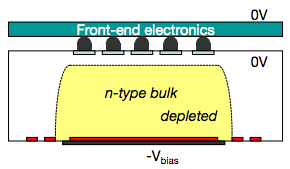
\includegraphics{figures/experiment/ATLAS_pixel_depletion_zones_normal}}
 	}
 	\hfill
 	\subfloat[ After type inversion.] {\label{fig:ATLAS-pixel-inverted}
 		\resizebox{0.45\textwidth}{!}{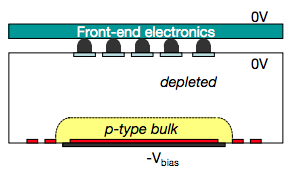
\includegraphics{figures/experiment/ATLAS_pixel_depletion_zones_inverted}}
 	}
 	\caption{Comparison of depletion zones in $n^+$-in-$n$ pixel sensors before and after type inversion. Before type inversion, the electrical field grows from the bottom side, reaching the pixel implants at full depletion. After type inversion, the depletion zone grows from the pixel side, allowing operation even if the bulk is not fully depleted.}
 	\label{fig:ATLAS-pixel}
 \end{figure}

 \begin{figure}[htbp]
 	\centering
 	\resizebox{0.5\textwidth}{!}{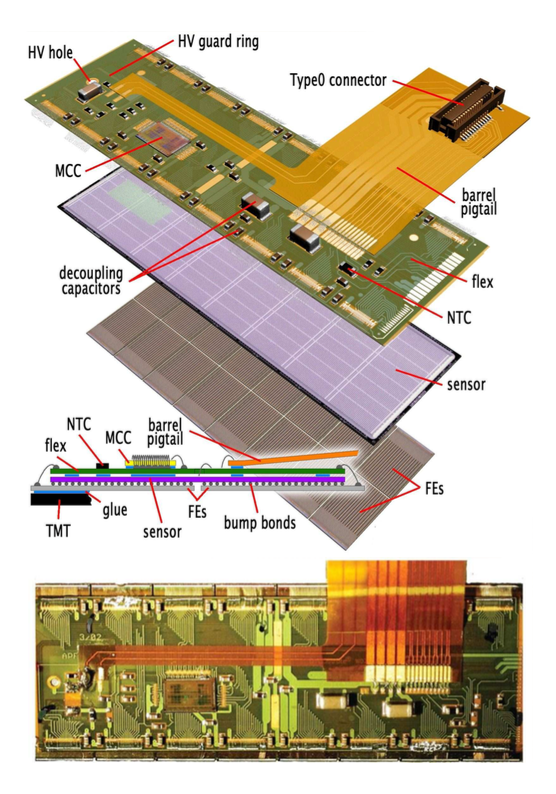
\includegraphics{figures/experiment/ATLAS_pixel_module}}
 	\caption{Schematic pictures of a barrel pixel module. The top diagram shows the assembly of a module, consisting of the front-end electronics chips (FEs), the pixel sensor elements, and the flex-hybrid, which bears the module control chip (MCC) and NTC thermistors. The bottom is a photograph of a barrel pixel module.}
 	\label{fig:ATLAS-pixel-module}
 \end{figure}
 
 

The pixel sensors are assembled into pixel modules, shown in figure~\ref{fig:ATLAS-pixel-module}. Each modules contains 16 front-end electronics chips each with 2880 electronics channels. The front-ends are bump bonded to the pixel sensor elements. The other side of the pixel sensor tile is glued to a flexible polyimide printed circuit board (\emph{flex-hybrid}) that houses the module control chip.

The layout of the pixel detector is summarized in table~\ref{table:ATLAS-pixel-layout}.  The modules are assembled into staves in the barrel region, each with 13 pixel modules, and sectors in the end-caps, each with 6 pixel modules. The barrel layers consist of 22, 38, and 52 staves for layers 0, 1, and 2, respectively, while the end-caps each contain eight sectors\footnote{During the shutdown following Run I, a fourth layer of barrel pixel detectors, known as the insertable B-layer (IBL), was added between the beam pipe and the innermost pixel layer. The data used in this dissertation predate the inclusion of the IBL.}. In the barrel, to provide complete coverage, the pixel staves overlap and are mounted with a tilt angle of $20^{\circ}$ between the normal to the module surface and $\hat{r}$, in the $\hat{\phi}$ direction. 

In the barrel, the pixels have an intrinsic accuracy of $\SI{10}{\micro\meter}$ in the $R-\phi$ direction and $\SI{115}{\micro\meter}$ in the $z$ direction, while in the end-caps, the intrinsic accuracy is $\SI{10}{\micro\meter}$ in the $R-\phi$ direction and $\SI{115}{\micro\meter}$ in the $R$ direction.

\begin{table}[htbp]
	\centering
	\begin{tabular}{|l|c|c|c|c|}
		\hline
		\textbf{Barrel} & \textbf{Radius (mm)} & \textbf{Staves} & \textbf{Modules} & \textbf{Pixels} \\
		\hline
		Layer-0 & $50.5$ & $22$ & $286$ & $13.2\times 10^6$ \\
		Layer-1 & $88.5$ & $38$ & $494$ & $22.8\times 10^6$ \\
		Layer-2 & $112.5$ & $52$ & $676$ & $31.2\times 10^6$ \\
		\hline
		\textbf{End-cap (one side)} & $z$ \textbf{(mm)} & \textbf{Sectors} & \textbf{Modules} & \textbf{Pixels} \\
		\hline
		Disk 1 & $495$ & $8$ & $48$ & $2.2\times 10^6$ \\
		Disk 2 & $495$ & $8$ & $48$ & $2.2\times 10^6$ \\
		Disk 3 & $495$ & $8$ & $48$ & $2.2\times 10^6$ \\
		\hline
		\textbf{Barrel and both end-caps} & & & $1744$ & $80.4\times 10^6$ \\
		\hline
	\end{tabular}
	\caption{Parameters of the pixel detector, from~\cite{TheATLASCollaboration:2008fg}.}
	\label{table:ATLAS-pixel-layout}
\end{table}

\subsubsection{SCT}\label{sec:ATLAS-id-sct}

The SCT consists of 15912 sensors using single-sided, $p$-in-$n$ type silicon strips. The use of single-sided strips lowers both the cost and the number of readout channels of the detector, which covers significantly more area than the pixel detector ($\SI{61.1}{\meter\tothe{2}}$ versus $\SI{2.3}{\meter\tothe{2}}$). In the barrel, the strips have a pitch of $\SI{80}{\micro\meter}$ and a length of $\SI{12}{\centi\meter}$. In the endcaps, the sensors are trapezoidal with radially arranged strips, with a mean strip pitch of $\SI{80}{\micro\meter}$ and a length of $\SI{12}{\centi\meter}$. Each sensor has 768 active strips. Like the pixel sensors, the operating voltage is initially $\sim$\SI{150}{\volt}, but will require an increase to \SIrange[range-phrase=-]{250}{350}{\volt} after several years of irradiation, depending on the location of the sensor. 

The SCT modules are shown in figure~\ref{fig:ATLAS-SCT-modules}.The 2112 barrel modules contain four sensors, while the 1976 end-cap modules contain two sensors. In both cases, the sensors are glued to a $\SI{380}{\micro\meter}$-thick thermal pyrolitic graphite (TPG) base-board. The sensors are assembled in two layers with a rotation of $\pm\SI{20}{\milli\radian}$ about the center of the sensors. The stereo angle between the two sensors allows for a measurement of the position along the length of the sensors. 

% Arrangement into barrel layers and end-caps

The intrinsic accuracy of the SCT sensors is $\SI{17}{\micro\meter}$ along the strip pitch, corresponding to the $R-\phi$ direction. Along the length of the strips, the stereo angle allows for position measurement with an accuracy of $\SI{580}{\micro\meter}$, corresponding to the $z$ direction in the barrel and the $R$ direction in the end-caps.

\begin{table}[htbp]
	\centering
	\scriptsize
	\begin{tabular}{|l|c|c|c|c|}
		\hline
		\textbf{Barrel layer} & \textbf{Radius (mm)} & \textbf{Length (mm)} & \textbf{Module tilt angle} & \textbf{Number of modules} \\
		\hline
		3 & $299$ & $1498$ & $11.00^{\circ}$ & $384$ \\
		4 & $371$ & & $11.00^{\circ}$ & $480$ \\
		5 & $443$ & & $11.25^{\circ}$ & $576$ \\
		6 & $514$ & & $11.25^{\circ}$ & $672$ \\
		\hline
	\end{tabular}
	\caption{The dimensions and arrangement of modules in the four SCT layers. The tilt angle is between the normal to the module surface and $\hat{r}$, in the $\hat{\phi}$ direction.}
	\label{fig:ATLAS-SCT-layout}
\end{table}

\begin{figure}[htbp]
	\centering
	\subfloat[] {
		\resizebox{0.4\textwidth}{!}{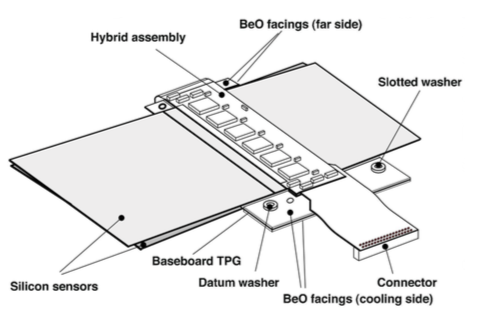
\includegraphics{figures/experiment/ATLAS_SCT_module_barrel}}
	}
	\hfill
	\subfloat[] {
		\resizebox{0.4\textwidth}{!}{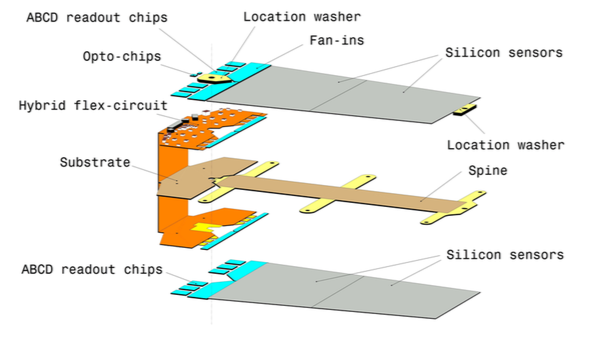
\includegraphics{figures/experiment/ATLAS_SCT_module_endcap}}
	}
	\caption{Diagrams of the SCT barrel (left) and end-cap (right) modules.}
	\label{fig:ATLAS-SCT-modules}
\end{figure}


\subsubsection{TRT}\label{sec:ATLAS-id-trt}

The TRT detector elements are polyimide drift (straw) tubes. The straws are arranged such that charged particles with $\pt > \SI{500}{\mega\electronvolt}$ and $|\eta|<2.0$ traverse at least 36 straws, except in the barrel/end-cap transition region where particles traverse as few as 22 straws. The straws are interleaved with polypropylene fibers in the barrel and polypropylene foils in the end-caps to provide transition radiation; electrons with $\pt>\SI{2.0}{\giga\electronvolt}$ typically leave $7$-$10$ high-threshold hits. The intrinsic resolution of the straws is $\SI{130}{\micro\meter}$ in the transverse direction.

The straws measure $\SI{4}{\milli\meter}$ in diameter and $\SI{144}{\centi\meter}$ ($\SI{37}{\centi\meter}$) in length in the barrel (end-caps). The straw walls consist of two $\SI{35}{\micro\meter}$ aluminum-coated polyamide films bonded back-to-back.
%The base film material is a $\SI{25}{\micro\meter}$ thick layer of polyamide, which is coated on the exterior side with a $\SI{0.2}{\micro\meter}$ thick layer of Al and a \SIrange[range-phrase=-]{5}{6}{\micro\meter} thick protective layer of graphite-polyamide. The other side of the film is coated with a \SIrange[range-phrase=-]{5}{6}{\micro\meter} thick layer of polyurethane, which is used to heat-seal the two film layers together. 
The anodes of the detectors are gold-plated tungsten wires running down the axis of the tubes, with $\SI{31}{\micro\meter}$ diameter.
% and plated with \SIrange[range-phrase=-]{0.5}{0.7}{\micro\meter} of gold. 
The wires are supported at the end of the straw by an end plug, where they connect to the front-end electronics. At the middle of the straw, the wires are supported by a plastic insert, and are also split electrically by a fused glass capillary to reduce occupancy. The active length of each half of the wire is $\SI{71.2}{\centi\meter}$, with a $\SI{2}{\centi\meter}$ inefficient section at the middle. 
%The signal attenuation length is $\sim$\SI{4}{\meter}, and the signal propagation time is $\sim$\SI[per-mode=fraction]{4}{\nano\second\per\meter}. 
The straws are filled with a mixture of 70\% Xe, 27\% CO$_2$, and $3\%$ O$_2$. With a cathode voltage of $\SI{-1530}{\volt}$, the gain in the straws is $2.5\times 10^4$.

The layout of the straws in the barrel and end-caps is summarized in table~\ref{table:ATLAS-TRT-layout}. In the barrel, the straws are arranged into three layers of modules as shown in figure~\ref{fig:ATLAS-TRT-barrel-modules}, with different dimensions and straw counts depending on the layer. The straws are interleaved with transition radiation material, polypropylene fibers measuring $\SI{19}{\micro\meter}$ in diameter. The module shell is made from $\SI{400}{\micro\meter}$ thick carbon fiber, and serve not only as a support structure, but also as a gas manifold for CO$_2$, which prevents high-voltage discharges, flushes any Xe leaking from the straws, and conducts heat away from the straws.  

The endcaps consist of 160 layers of 768 straws, arranged radially into 20 wheels with 8 layers each. The inner 12 wheels (type-A) are spaced $\SI{8}{\milli\meter}$ in $z$, while the outer 8 wheels (type-B) are spaced by $\SI{15}{\milli\meter}$. Each successive layer in a wheel is separated by a $\SI{15}{\micro\meter}$ thick polypropylene radiator foil, and is rotated by $3/8$ of the azimuthal straw spacing to optimize the uniformity of the number of straw crossed.


\begin{table}[htbp]
	\centering
	\begin{tabular}{|l|c|c|c|c|c|}
		\hline
		 & $z$ (mm) & $R$ (mm) & Modules & Layers & Straws/Module \\
		 \hline
		 \textbf{Barrel (both sides)} & $\mathbf{0\mhyphen780}$ & $\mathbf{554\mhyphen1082}$ & $\mathbf{96}$ & $\mathbf{73}$ & $\mathbf{52544}$ \\
		 Type-1 module (inner) & $400\mhyphen712.1$ & $563\mhyphen624$ & \multirow{2}{*}{$32$} & $9$ & \multirow{2}{*}{$329$} \\
		 Type-1 module (outer) & $7.5\mhyphen712.1$ & $625\mhyphen 694$ & & $10$ & \\
		 Type-2 module & $7.5\mhyphen 712.1$ & $697\mhyphen860$ & $32$ & $24$ & $520$ \\
		 Type-3 module & $7.5\mhyphen 712.1$ & $863\mhyphen 1066$ & $32$ & $30$ & $793$ \\
		 \hline
		 \textbf{End-cap (one side)} & $\mathbf{827\mhyphen 2744}$ & $\mathbf{615\mhyphen1106}$ & $\mathbf{20}$ & $\mathbf{160}$ & $\mathbf{122880}$ \\
		 Type-A wheels & $848\mhyphen1705$ & $644\mhyphen1004$ & $12$ & $8$ & $6144$ \\
		 Type-B wheels & $1740\mhyphen2710$ & $644\mhyphen1004$ & $8$ & $8$ & $6144$ \\
		 \hline
	\end{tabular}
	\caption{Layout and straw counts of the TRT barrel modules and end-cap wheels. The totals for the barrel and end-caps, shown in bold, include services and electronics.}	
	\label{table:ATLAS-TRT-layout}
\end{table}

\begin{figure}[htbp]
	\centering
	\resizebox{0.6\textwidth}{!}{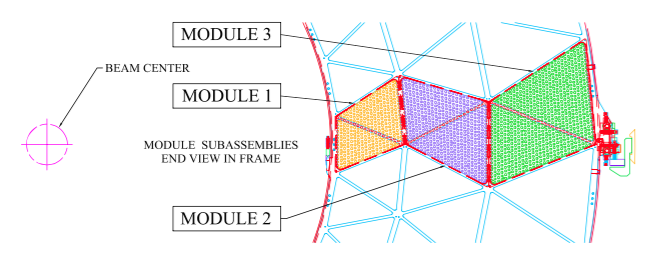
\includegraphics{figures/experiment/ATLAS_TRT_barrel_phistack}}
	\caption{Layout of the TRT barrel modules in the $R$-$\phi$ plane.}
	\label{fig:ATLAS-TRT-barrel-modules}
\end{figure}



\subsection{Calorimetry}\label{sec:ATLAS-calorimeters}
The calorimeter system occupies the volume directly exterior to the solenoid magnet, and measures the energy of electrons, photon, and hadrons up to a pseudorapidity of $|\eta|=4.9$. The arrangement of the calorimeters is shown in figure~\ref{fig:ATLAS-calorimeters}. The system consists of a number of independent sampling calorimeters. The electromagnetic calorimeter measures the energy of electrons and photons using lead and liquid argon (LAr) to measure the energy of electrons and photons. The hadronic calorimeter measures the energy of hadrons using steel and scintillator tiles in the barrel and copper and LAr in the end-caps. Finally, electromagnetic and hadronic calorimetry is performed in the forward region using copper-LAr and tungsten-LAr technology. Besides performing energy measurements, the calorimeters stop electrons, photons, and hadrons, providing shielding for the muon spectrometer. The total amount of material in front of and in the calorimeters is shown in terms of radiation lengths, $X_0$, and interaction lengths, $\lambda$, in figures~\ref{fig:ATLAS-calorimeters-X0} and \ref{fig:ATLAS-calorimeters-lambda0}.

\begin{figure}[htbp]
	\centering
	\resizebox{0.7\textwidth}{!}{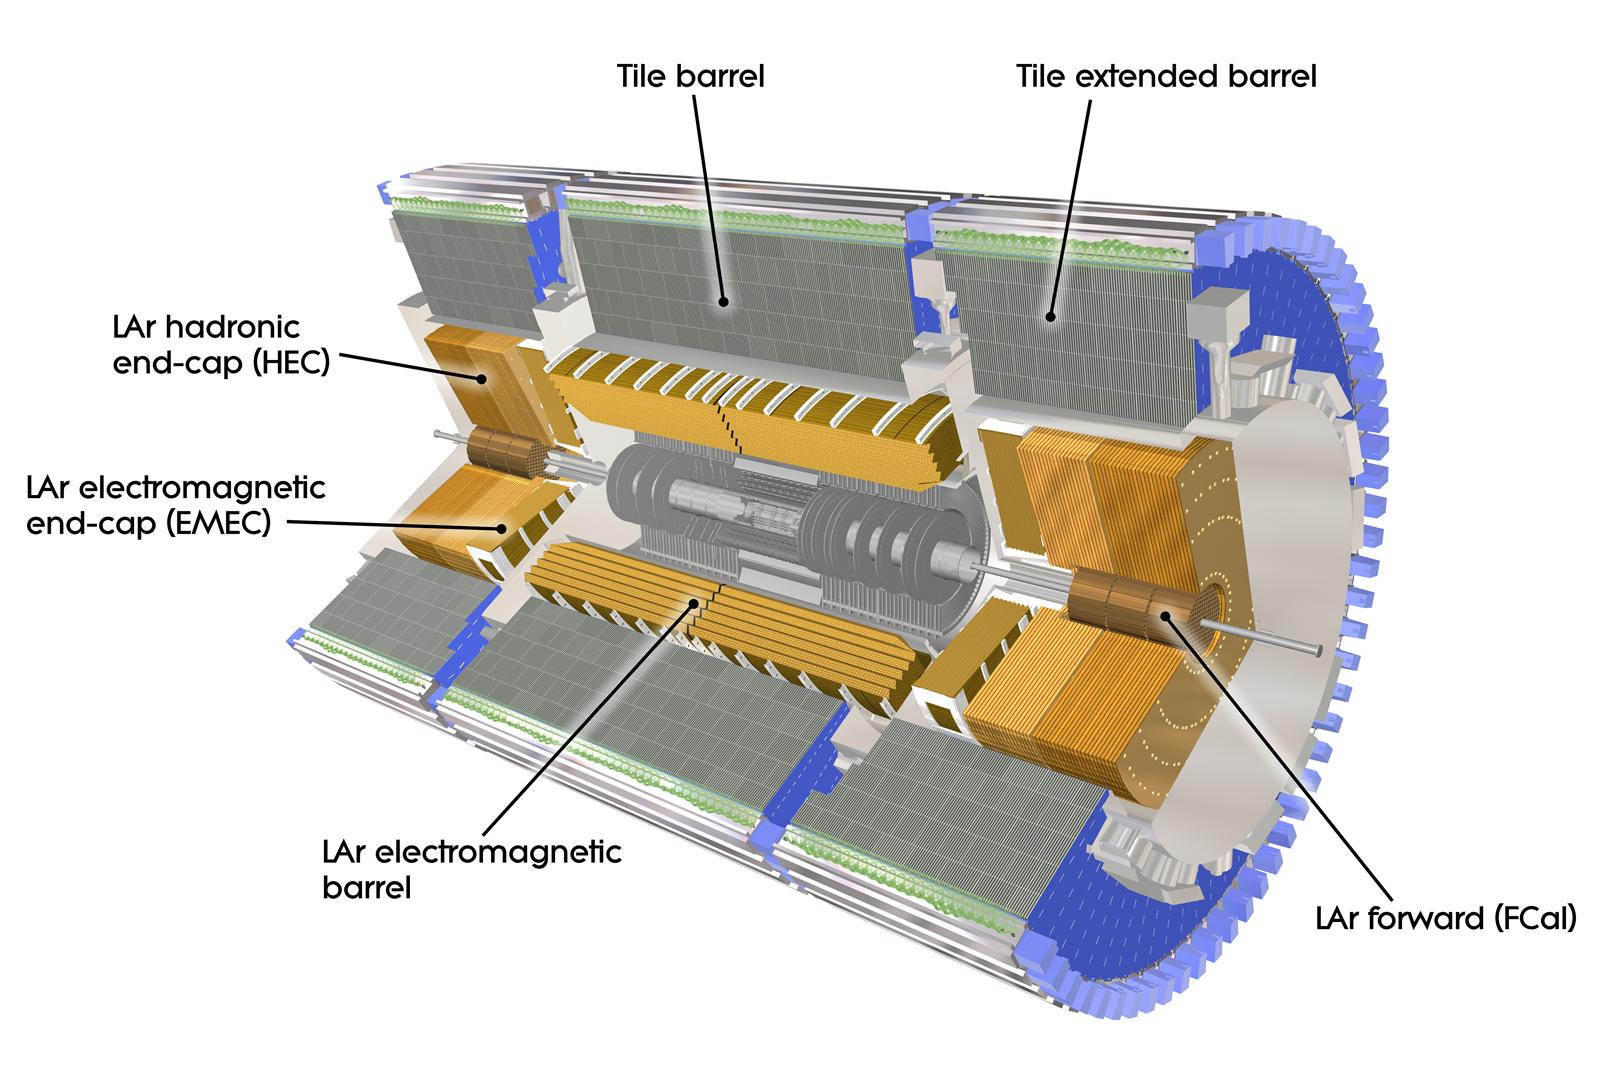
\includegraphics{figures/experiment/ATLAS_calorimeters_sketch}}
	\caption{A 3D model of the ATLAS calorimeters, showing the electromagnetic barrel and end-caps, hadronic barrel and end-caps, and the forward calorimeter.}
	\label{fig:ATLAS-calorimeters}
\end{figure}

\begin{figure}
	\centering
	\subfloat[ Material before the calorimeters.] {
		\resizebox{0.45\textwidth}{!}{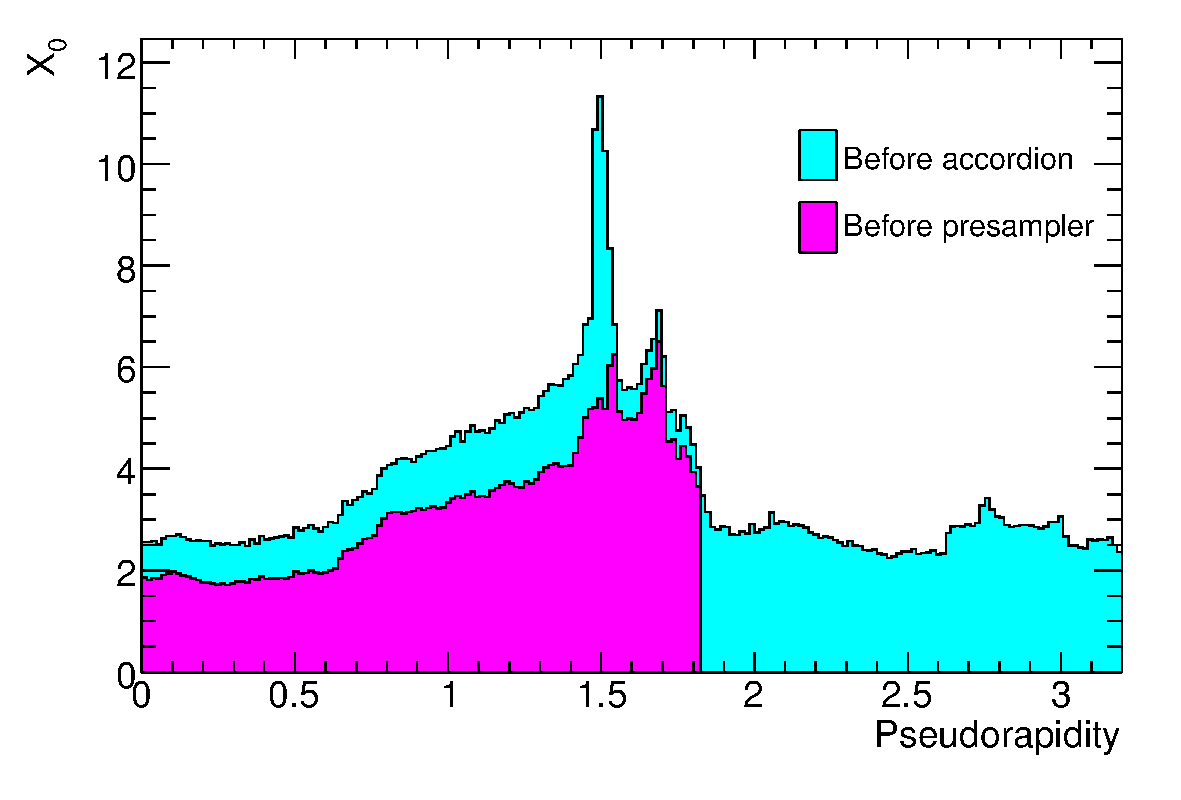
\includegraphics{figures/experiment/x0_before_calo_csc03}}
	}\hfill
	\subfloat[ Material in the crack region between the barrel and end-cap cryostats.] {
		\resizebox{0.45\textwidth}{!}{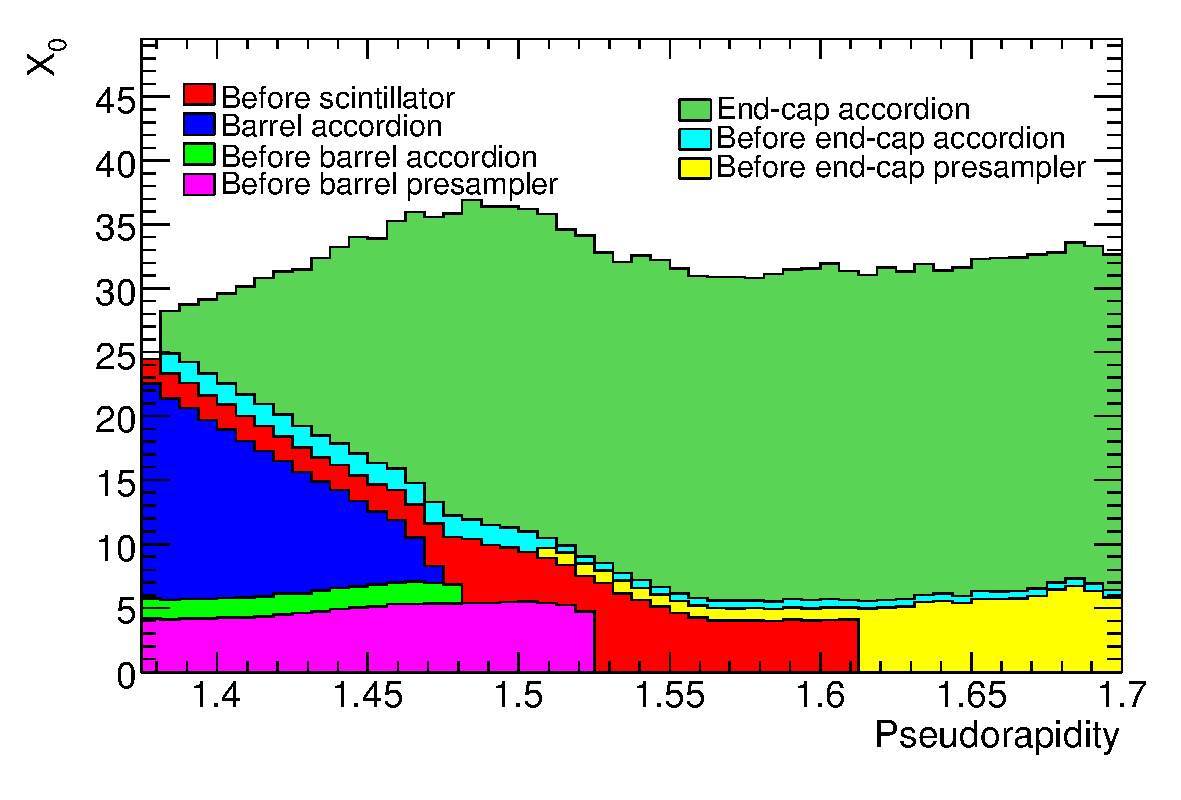
\includegraphics{figures/experiment/x0_crack_csc03}}
	} \\
	\subfloat[ Material in and before the barrel LAr calorimeter.] {
		\resizebox{0.45\textwidth}{!}{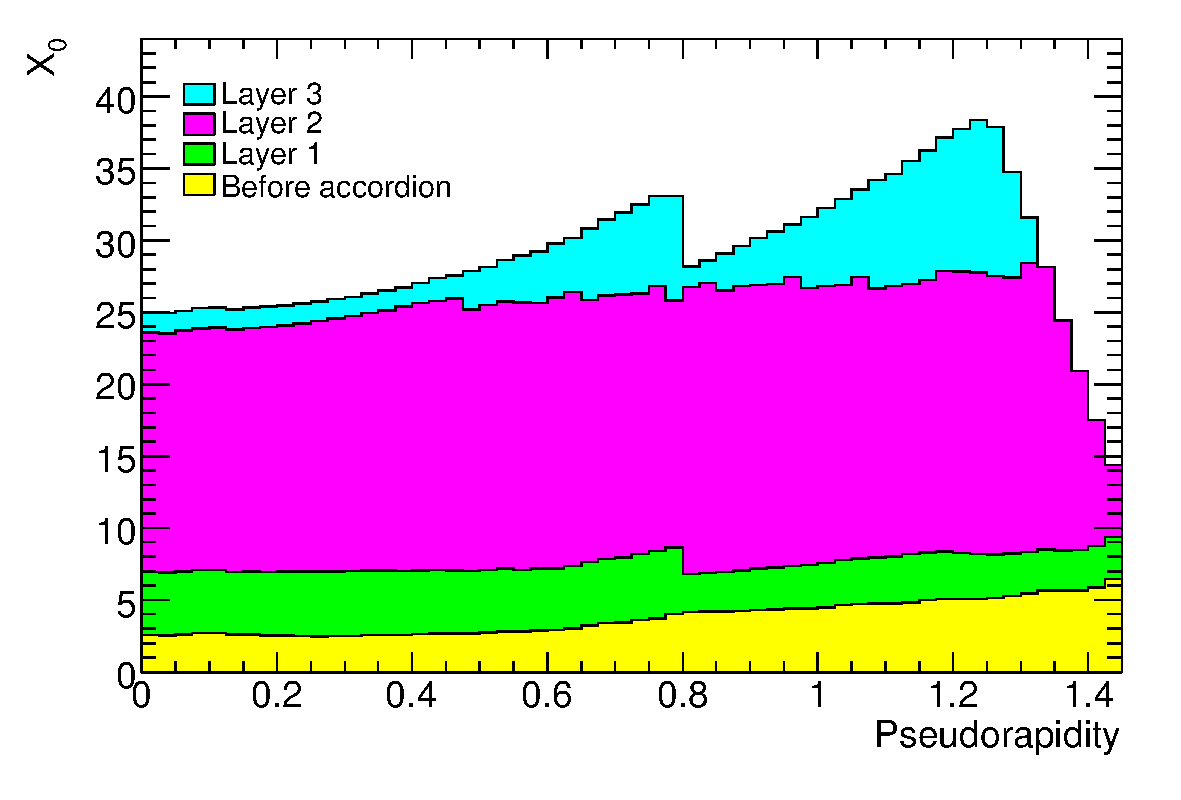
\includegraphics{figures/experiment/x0_layers_barrel_csc03}}
	}\hfill
	\subfloat[ Material in and before the end-cap LAr calorimeters.] {
		\resizebox{0.45\textwidth}{!}{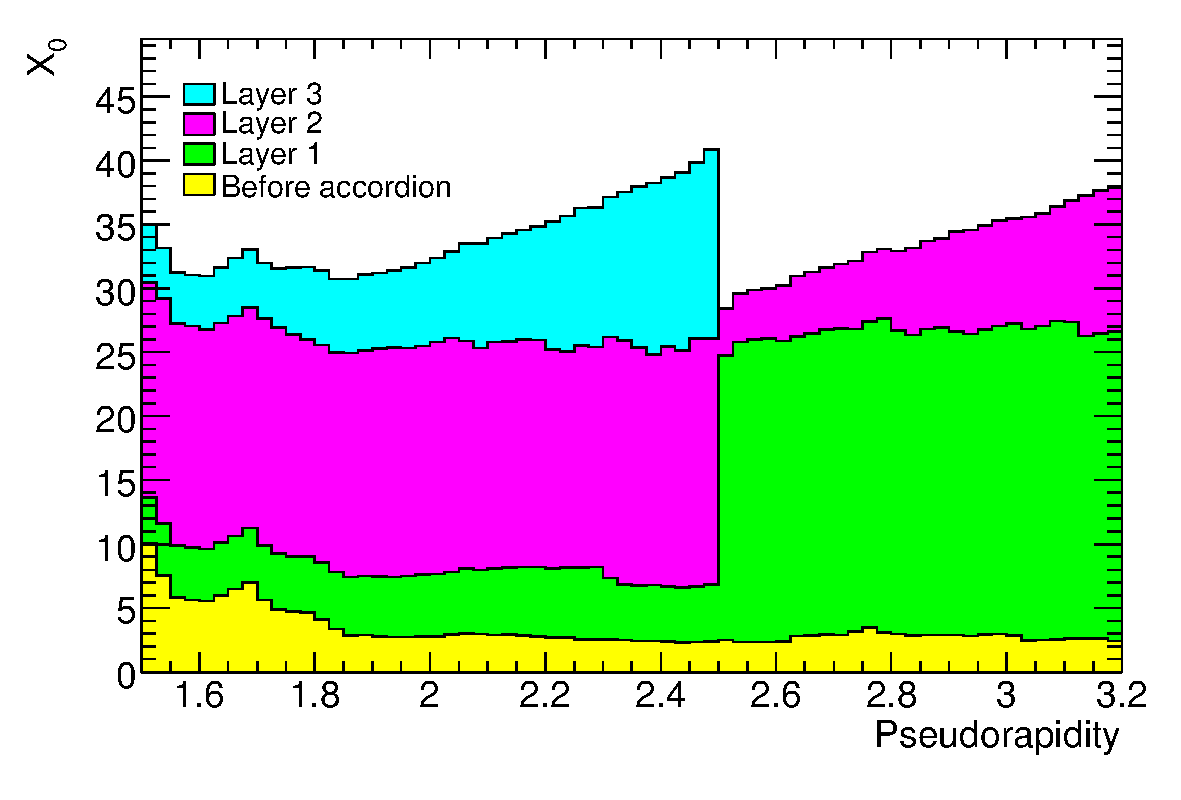
\includegraphics{figures/experiment/x0_layers_endcap_csc03}}
	}
	\caption{Cumulative amounts of material versus $|\eta|$ in front of and within the LAr electromagnetic calorimeter, in terms of radiation lengths, $X_0$.}
	\label{fig:ATLAS-calorimeters-X0}
\end{figure}

\begin{figure}
	\centering
	\resizebox{0.6\textwidth}{!}{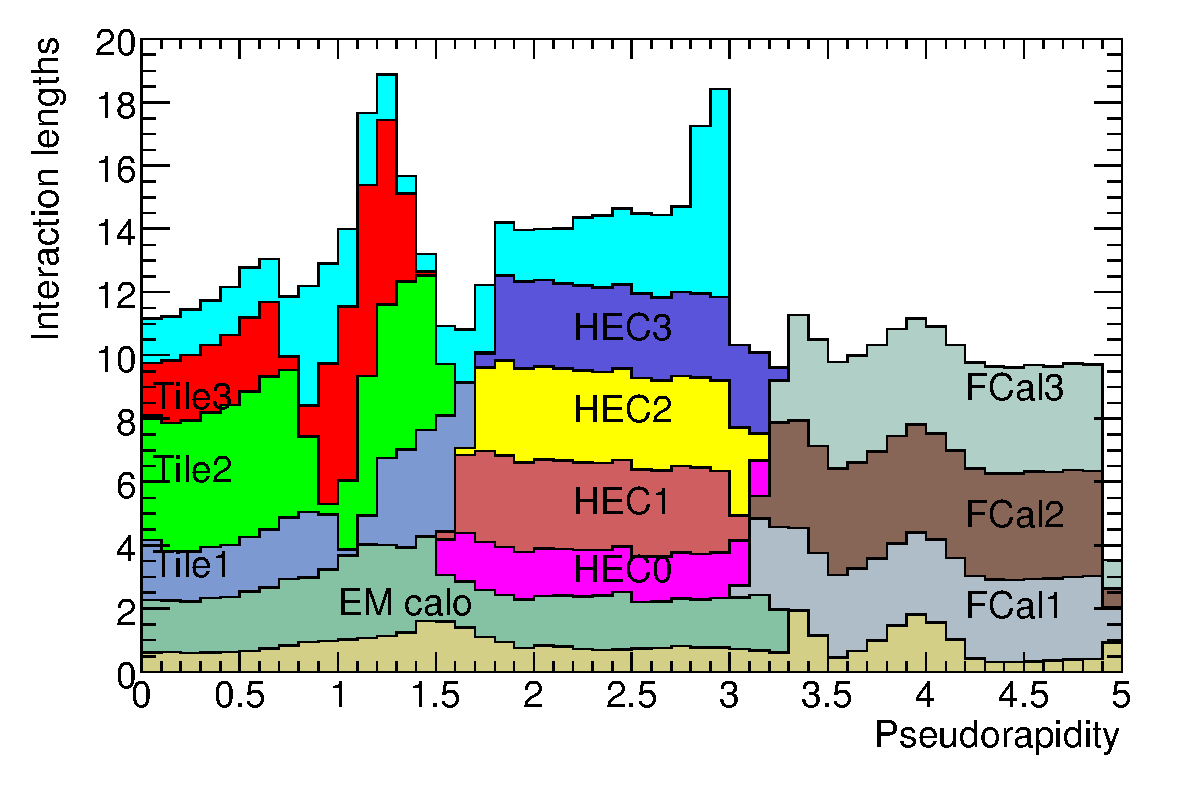
\includegraphics{figures/experiment/lambda_csc03}}
	\caption{Cumulative amounts of material versus $|\eta|$ due to each calorimeter in terms of interaction lengths, $\lambda$. The material in front of the calorimeters is also shown in tan.}
	\label{fig:ATLAS-calorimeters-lambda0}
\end{figure}



\subsubsection{Electromagnetic Calorimeter}\label{sec:ATLAS-calorimeters-ecal}

The electromagnetic calorimeter consists of two half-barrels ($0<\eta<\pm1.475$), two end-caps ($\pm1.375<\eta<\pm3.2$), and a presampler ($|\eta|<1.8$). The half-barrels and end-caps use LAr as the active material and steel-clad lead plates as the absorber. The lead plates are arranged in an accordion geometry to provide a uniform, gapless coverage in $\phi$, shown for a barrel module in figure~\ref{fig:ATLAS-LAr-module}. The plates are interleaved with electrodes built from copper etchings on polymide, consisting of three conducting layers. The outer conductive layers of the electrodes distribute the $\SI{2000}{\volt}$ high voltage over the electrode surface, which drifts the charges induced by ionization in the LAr towards the electrodes with a drift time of $\SI{450}{\nano\second}$. The inner layer of the electrode, separated from the outer layers by isolating foils, collects the signals via capacitive coupling. 

\begin{figure}[htbp]
	\centering
	\subfloat[ A LAr barrel module.] {
		\resizebox{0.45\textwidth}{!}{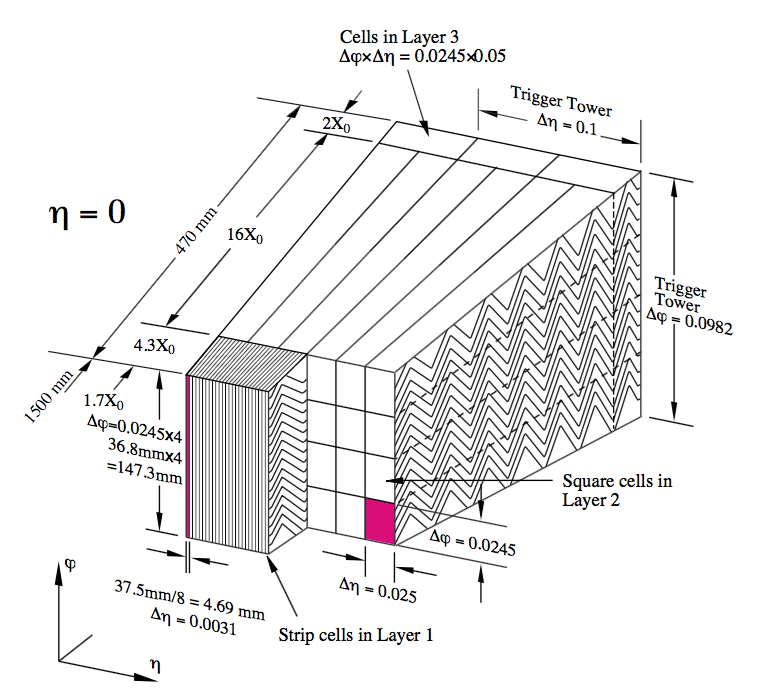
\includegraphics{figures/experiment/ATLAS_LAr_module}}
	}
	\subfloat[ Closeup image of the LAr accordion geometry.] {
		\resizebox{0.45\textwidth}{!}{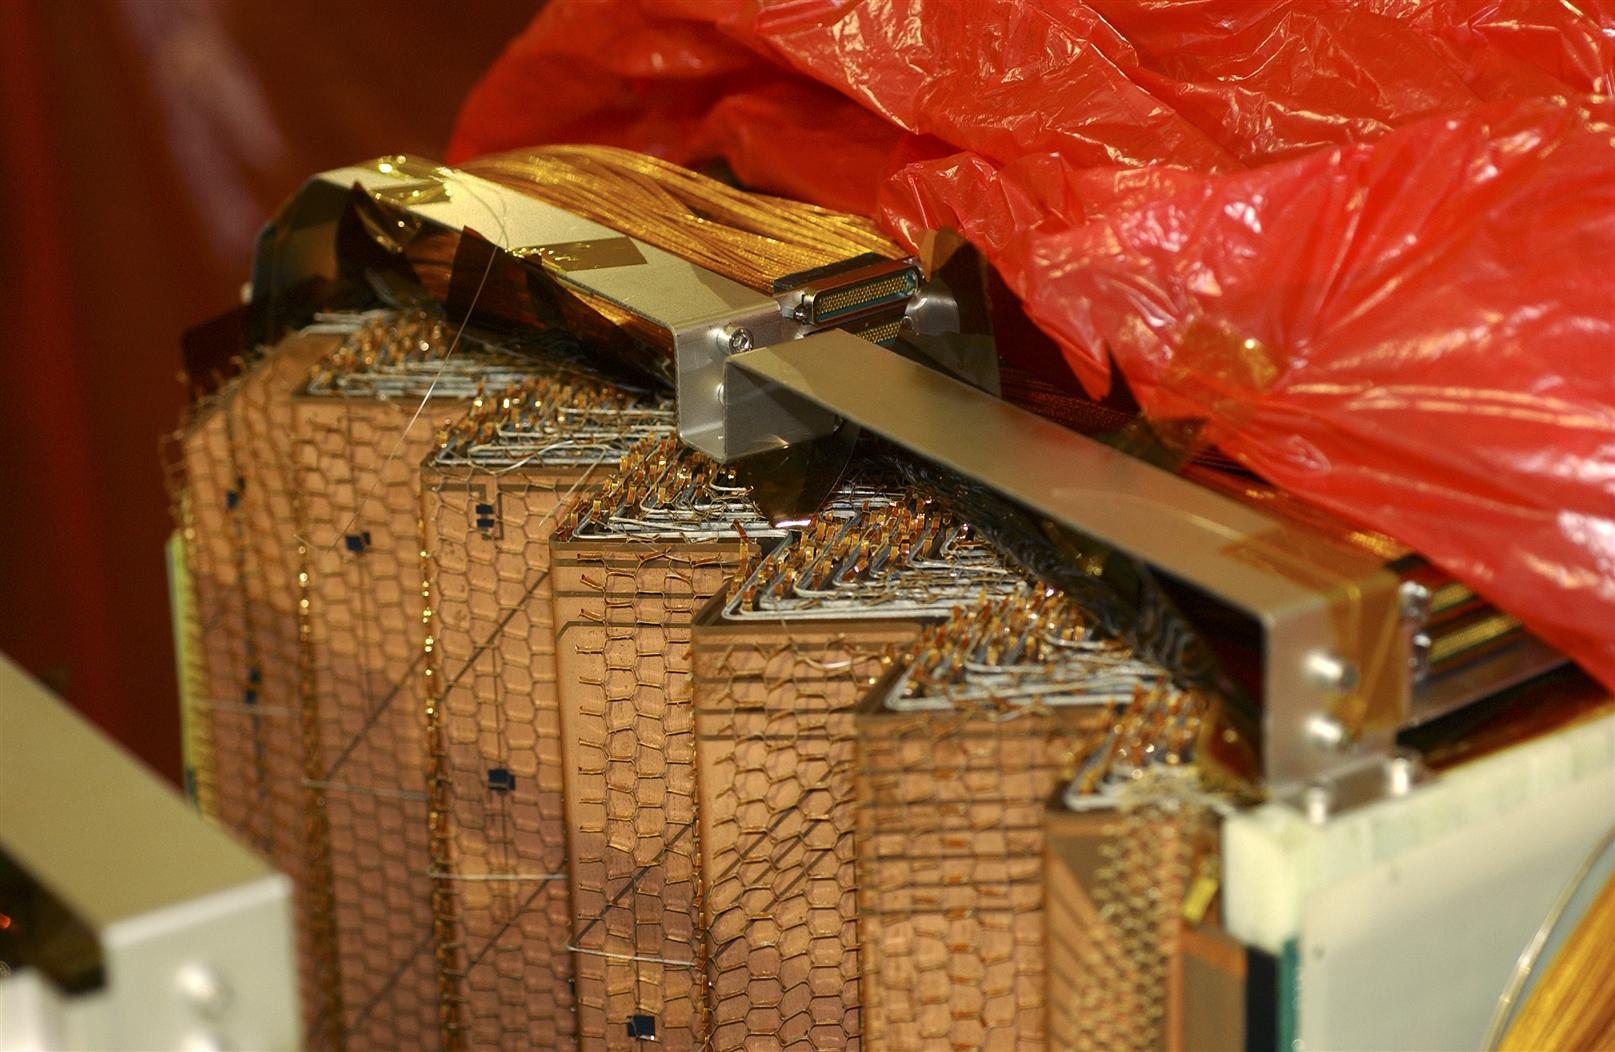
\includegraphics{figures/experiment/ATLAS_LAr_zigzags}}
	}
	\caption{The LAr calorimeter uses an accordion geometry to provide uniform coverage in $\phi$. Steel-clad lead plates are interleaved with electrodes, consisting of three copper layers separated by polyamide sheets. The barrel module is divided into three layers in depth, with fine segmentation in $\eta$ in the layer closest the interaction point.}
	\label{fig:ATLAS-LAr-module}
\end{figure}

The two half-barrels occupy the region $\SI{2.8}{\meter}<R<\SI{4}{\meter}$ and $\SI{0}{\meter}<z<\pm\SI{3.2}{\meter}$, which covers up to $|\eta|<1.52$ depending on the layer. Each half-barrel has 1024 lead plates with a thickness of $\SI{1.53}{\milli\meter}$ for $|\eta|<0.8$ and $\SI{1.13}{\milli\meter}$ for $|\eta|>0.8$. The cells are divided into three layers, and have variable size in $\eta$ and $\phi$:

\begin{itemize}
	\item The first layer is finely segmented in $\eta$ to improve the spatial resolution; this improves the particle identification, helps resolve nearby particles (in particular photon pairs from $\pi^0$ decays), and, in combination with the second layer, allows for a measurement of particle trajectories. The majority of the cells measure $\Delta\eta\times\Delta\phi=0.025/8\times0.1$. Cells in the barrel-end-cap over lap region, $1.40<|\eta|<1.475$, have a coarser granularity of $\Delta\eta\times\Delta\phi=0.025\times0.025$.

	\item The second layer absorbs most of the energy of the electromagnetic showers. Most of the cells have size $\Delta\eta\times\Delta\phi=0.025\times0.025$, except for cells with $1.40<|\eta|<1.475$, which measure $\Delta\eta\times\Delta\phi=0.075\times0.025$.

	\item The third layer aborbs the tails of electromagnetic showers, and has a coarse granularity of $\Delta\eta\times\Delta\phi=0.050\times0.025$.
\end{itemize}


%A LAr half barrel is shown in figure~\ref{fig:LAr-barrel}, prior to installation.

%\begin{figure}[htbp]
%	\centering
%	\resizebox{0.4\textwidth}{!}{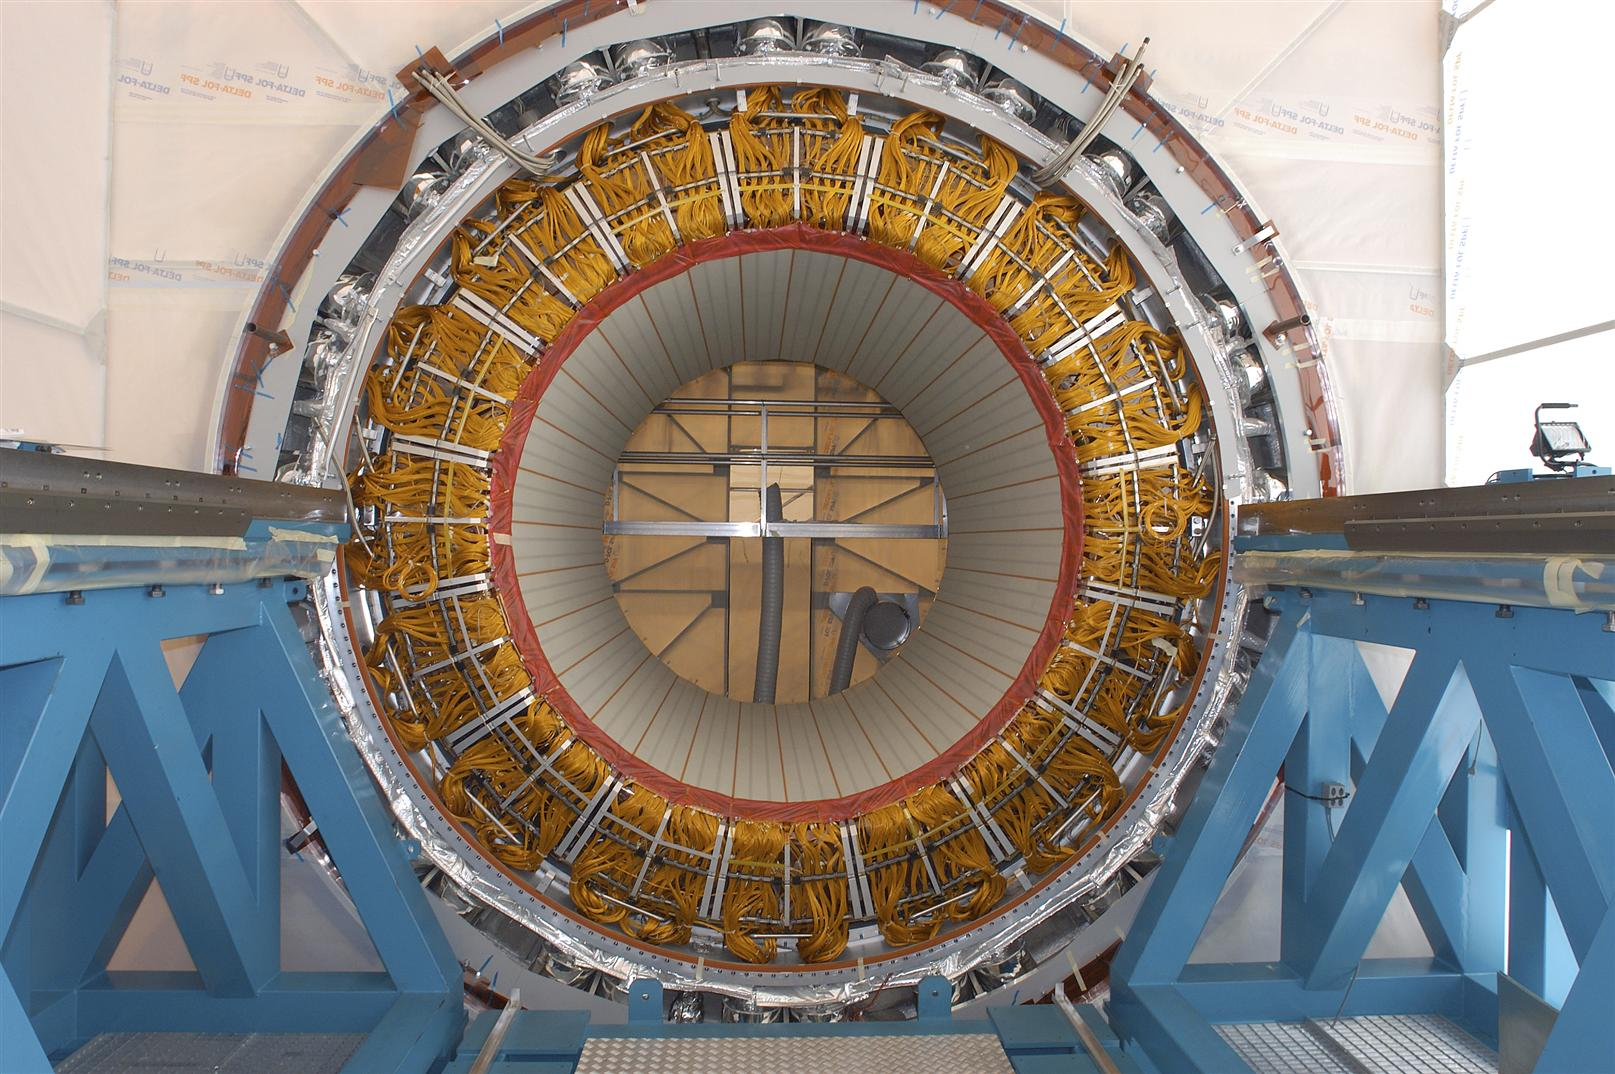
\includegraphics{figures/experiment/ATLAS_LAr_barrel}}
%	\caption{Photograph of a LAr calorimeter half-barrel, prior to installation.}
%	\label{fig:LAr-barrel}
%\end{figure}


The end-caps, one on either side of the interaction region, measure $\SI{63}{\centi\meter}$ in thickness with inner and outer radii of $\SI{33}{\centi\meter}$ and $\SI{209.8}{\centi\meter}$, respectively. 
%Each end-cap contains two co-axial sub-wheels, divided by a $\SI{3}{\milli\meter}$ gap at $|\eta|=2.5$.
%The inner and outer wheels contain 256 and 768 lead absorbers, respectively, 
Each end-cap consists of 1024 lead absorbers with the same accordion geometry as used in the barrel. In the region $1.5<|\eta|<2.5$, the end-caps present three layers in the longitudinal direction, with fine $\eta$ segmentation in the front layer. At $|\eta|=1.5,$ the granularity of each layer is the same as in the barrel, becoming coarser in the first layer with increasing $|\eta|$. Elsewhere, there are two longitudinal layers with coarser transverse granularity.

Finally, the presampler is an instrumented layer of LAr installed in front of the first layer calorimeter, with a thickness of $\SI{11}{\milli\meter}$ in the barrel ($|\eta|<1.5$) and $2\times \SI{2}{\milli\meter}$ in the end-caps ($1.5<|\eta|<1.8$). The presampler measures the energy lost due to interactions with material between the interaction region and the calorimeters (the beam pipe, inner detector, solenoid, cryostates, and other services and support structures). The total amount of material before and in the electromagnetic calorimeters is shown in figure~\ref{fig:ATLAS-calorimeters-X0} in terms of radiation lengths, $X_0$. The cells have a granularity of $\Delta\eta\times\Delta\phi=0.025\times0.1$. 

% Conclusion
In total, the electromagnetic calorimeter has 101,760 readout channels for the barrel, 62,208 channels for the end-caps, 7,808 channels for the barrel presampler, and 1,536 channels for the end-cap presamplers. 


%\begin{table}[htbp]
%	\centering
%	\begin{tabular}{|l|c|c|}
%		\hline
%		Layer & $\eta$ range & Granularity $\Delta\eta\times\Delta\phi$ \\
%		\hline
%		Barrel presampler & $|\eta|<1.52$ & $0.025\times0.1$ \\
%		\hline
%		\multirow{2}{*}{Barrel 1} & $|\eta|<1.40$ & $0.025 / 8 \times 0.1$ \\
%		 & $1.40<|\eta|<1.475$ & $0.025\times0.025$ \\
%		\hline
%		\multirow{2}{*}{Barrel 2} & $|\eta|<1.40$ & $0.025\times0.025$ \\
%		 & $1.40<|\eta|<1.475$ & $0.075\times 0.025$ \\
%		\hline
%		Barrel 3 & $|\eta|<1.35$ & $0.050\times0.025$ \\
%		\hline
%		\hline
%		\multirow{7}{*}{End-cap 1} & $1.375<|\eta|<1.425$ & $0.050\times0.1$ \\
%		 & $1.425<|\eta|<1.5$ & $0.025\times0.1$ \\
%		 & $1.5<|\eta|<1.8$ & $0.025/8\times0.1$ \\
%		 & $1.8<|\eta|<2.0$ & $0.025/6\times0.1$ \\
%		 & $2.0<|\eta|<2.4$ & $0.025/4\times0.1$ \\
%		 & $2.4<|\eta|<2.5$ & $0.025\times0.1$ \\
%		 & $2.5<|\eta|<3.2$ & $0.1\times0.1$ \\
%		\hline
%		\multirow{3}{*}{End-cap 2} & $1.375<|\eta|<1.425$ & $0.050\times0.025$ \\
%		 & $1.425<|\eta|<2.5$ & $0.025\times0.025$ \\
%		 & $2.5<|\eta|<3.2$ & $0.1\times0.1$ \\
%		\hline
%		End-cap 3 & $1.5<|\eta|<2.5$ & $0.050\times0.025$ \\
%		\hline
%	\end{tabular}
%	\caption{Granularity of each layer of the LAr electromagnetic calorimeter.}
%	\label{table:ATLAS-LAr-segmentation}
%\end{table}


\subsubsection{Tile Calorimeter}\label{sec:ATLAS-calorimeters-tile}
The tile calorimeter performs hadronic calorimetry in the region $|\eta|<1.7$, occupying the radial range $\SI{2.28}{\meter}<R<\SI{4.25}{\meter}$. Divided into a $\SI{5.8}{\meter}$-long central barrel and two $\SI{2.6}{\meter}$-long extended barrels on either side, it uses steel as the absorber and scintillating tiles as the active material. The total depth is approximately $7.4\lambda$. 

Each of the three calorimeter sections is divided azimuthally into 64 modules, each spanning $\Delta\phi=5.625$. A module is shown schematically in figure~\ref{fig:ATLAS-calorimeters-tile-module}. The outer edge of a module is a steel girder which houses the tile calorimeter readout electronics and also provides flux return for the solenoidal magnetic field. The body of the module is a self-supporting structure built from steel absorber plates, with $\SI{4}{\milli\meter}$-thick spacer plates glued in staggered fashion to $\SI{5}{\milli\meter}$-thick master plates. The staggered spacing creates the gaps into which the scintillating tiles are inserted, with a steel-to-scintillator volume ratio of approximately $4.7:1$. 

The scintillating tiles use polystyrene as the base material, in which ionizing particles induce the production of ultraviolet light. The polystyrene is doped with wavelength-shifting fluors, 1.5\% PTP and 0.044\% POPOP, which convert the scintillation light into the visible light. The tiles measure $\SI{3}{\milli\meter}$ thick, and vary between \SIrange[range-phrase=-]{97}{187}{\milli\meter} in radial length and \SIrange[range-phrase=-]{200}{400}{\milli\meter} in azimuthal length. A plastic sleeve envelops each tile, both for the protection of the tile during installation and also to improve the scintillation light collection efficiency due to a reflectivity of $\sim 95\%$. At the tile edges, wavelength-shifting fibers transmit the light to photomultiplier tubes housed in the girder. The grouping of the fibers determines the readout cell size, as shown in figure~\ref{fig:ATLAS-calorimeters-tile-cell-layout}; the cells measure $\Delta\eta\times\Delta\phi=0.1\times0.1$ in the transverse direction, and are segmented into three layers longitudinally corresponding to depths of approximately $1.5\lambda$, $4.1\lambda$, and $1.8\lambda$.


\begin{figure}[htbp]
	\centering
	\subfloat[] {\label{fig:ATLAS-calorimeters-tile-module}
		\resizebox{0.35\textwidth}{!}{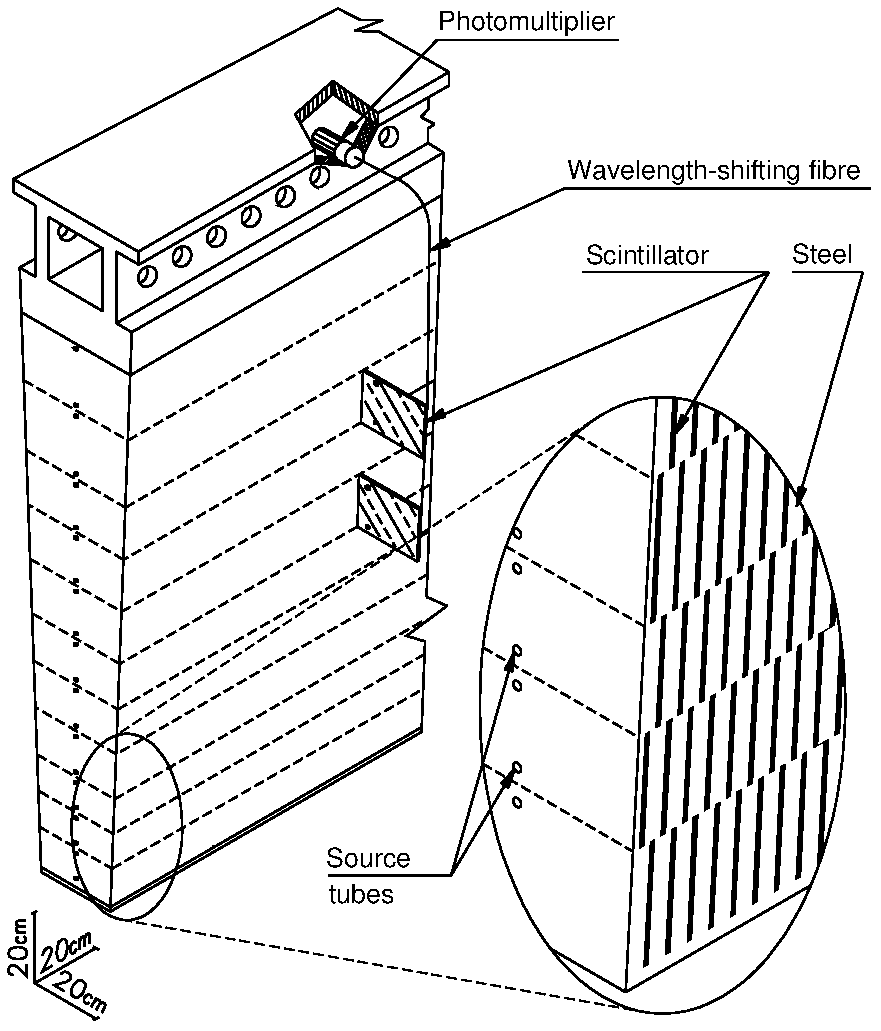
\includegraphics{figures/experiment/ATLAS_TILE_module}}
	}
	\hfill
	\subfloat[] {\label{fig:ATLAS-calorimeters-tile-cell-layout}
		\resizebox{0.55\textwidth}{!}{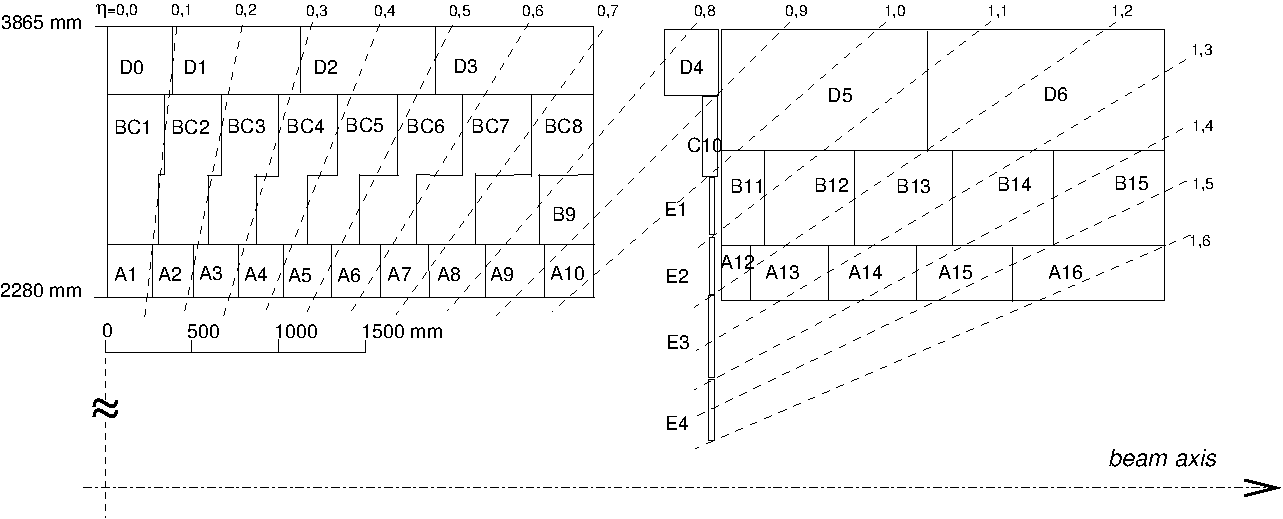
\includegraphics{figures/experiment/ATLAS_TILE_cell_layout}}
	}
	\caption{Left: Schematic view of a tile calorimeter module, showing assembly of the steel absorber, the inserted scintillator tiles, and the readout of lighting through wavelength-shifting fibers to the photomultiplier tubes. Right: Layout of the tile calorimeter cells, defined by the grouping of the readout fibers connecting the scintillating tiles to the photomultiplier tubes.}
	\label{fig:ATLAS-calorimeters-tile}
\end{figure}



\subsubsection{Hadronic End-Cap Calorimeters}\label{sec:ATLAS-calorimeters-HEC}
Outside the tile calorimeter, two hadronic end-cap calorimeters (HEC) perform hadronic calorimetry in the pseudorapidity range $1.5<|\eta|<3.2$. The HECs use copper and LAr arranged into a flat plate geometry, as shown in figure~\ref{fig:ATLAS-calorimeters-HEC-layout}. Each HEC consists of two wheels (HEC1 and HEC2), which are further divided into two longitudinal segments.  The plates have an inner radius of $\SI{372}{\milli\meter}$ or $\SI{475}{\milli\meter}$ depending on $z$, and an outer radius of $\SI{2030}{\milli\meter}$. HEC1 contains 24 copper plates, each $\SI{24}{\milli\meter}$ thick and spaced by $\SI{8.5}{\milli\meter}$, plus a $\SI{12.5}{\milli\meter}$-thick front plate. HEC2 contains 16 copper plates measuring $\SI{50}{\milli\meter}$ in thickness, with a $\SI{25}{\milli\meter}$-thick front plate. The sampling fractions are thus $4.4\%$ for HEC1 and $2.2\%$ for HEC2. 

The gaps contain 3 electrodes spaced by $\SI{1.8}{\milli\meter}$, the outer two of which supply a nominal operating voltage of $\SI{1800}{\volt}$, and the middle of which performs the readout. The readout pads provide a transverse segmentation of $\Delta\eta\times\Delta\phi=0.1\times0.1$ for $|\eta|<2.5$, and $\Delta\eta\times\Delta\phi=0.2\times0.2$ for $2.5<|\eta|<3.2$. In total, 5,632 channels are read from the HEC. 

\begin{figure}[htbp]
	\centering
	\resizebox{0.6\textwidth}{!}{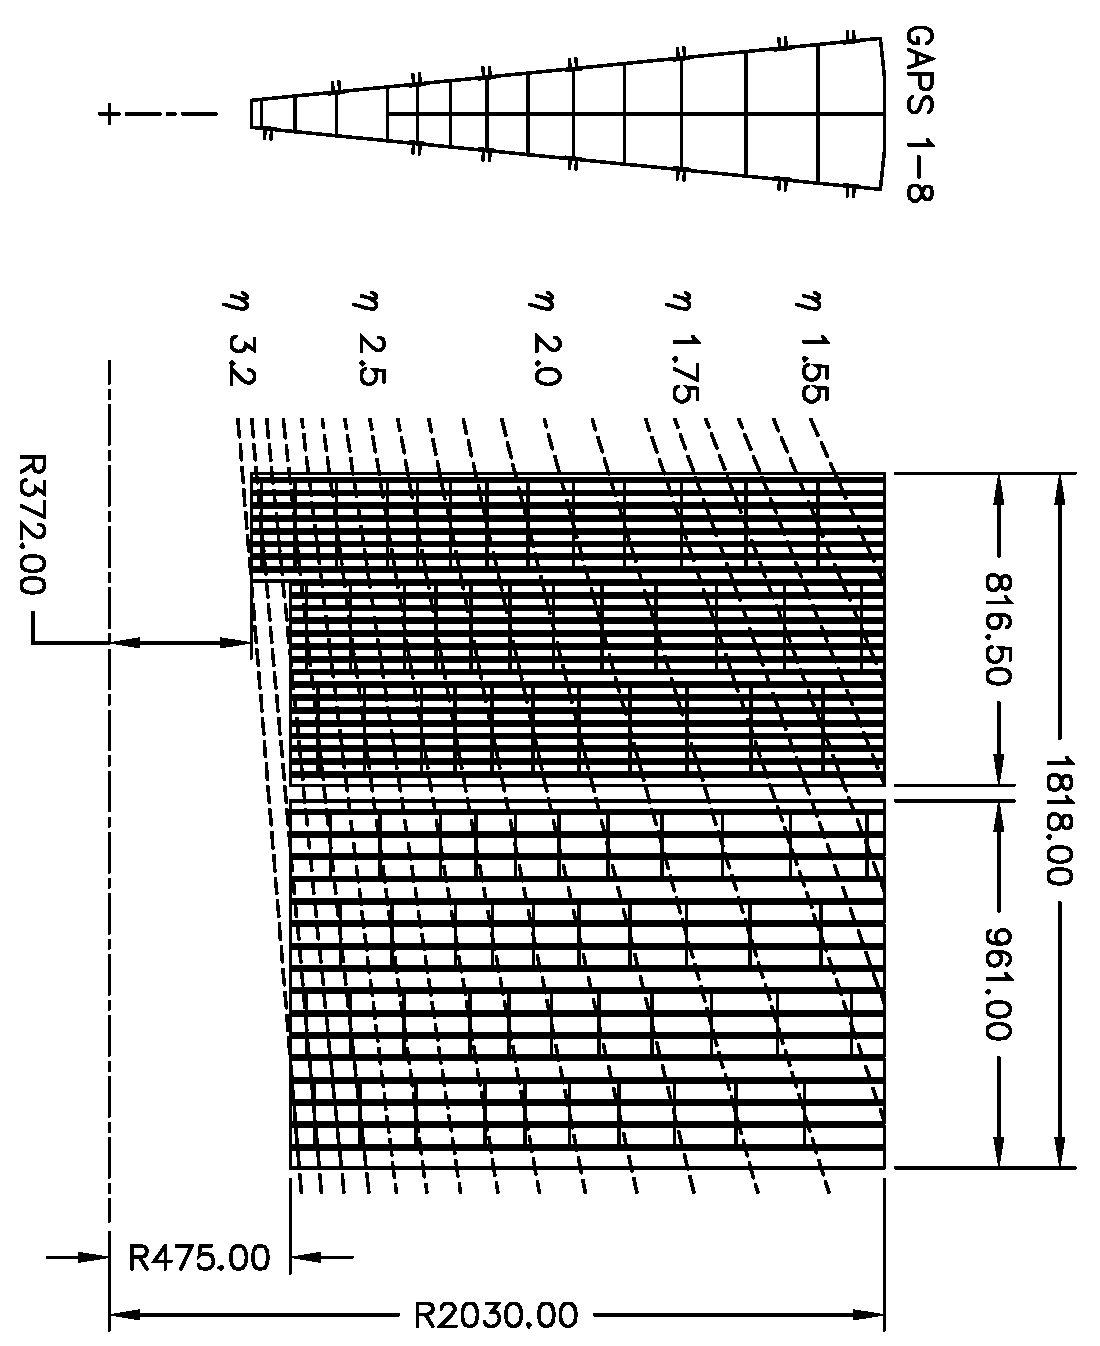
\includegraphics[angle=90]{figures/experiment/ATLAS_HEC_layout}}
	\caption{Schematic $R-\phi$ (left) and $R-z$ (right) views of the hadronic end-cap calorimeters.}
	\label{fig:ATLAS-calorimeters-HEC-layout}
\end{figure}


\subsubsection{Forward Calorimeter}\label{sec:ATLAS-calorimeters-fcal}
The forward calorimeter (FCal) performs both electromagnetic and hadronic calorimetry in the very forward region, $3.2<|\eta|<4.9$, and also shields the muon system from high particle fluxes. On each side, the FCal is divided into three layers measuring $\SI{45}{\centi\meter}$ in depth, an electromagnetic layer (FCal1) and two hadronic layers (FCal2 and FCal 3). All three layers use LAr as the active medium, with very thin gaps due to avoid ion buildup due to the high particle flux. FCal1 uses copper absorbers to optimize the resolution and heat removal. FCal2 and FCal3 use tungsten absorbers, which provides good containment and reduces the lateral spread of hadronic showers. Finally, a passive brass plug behind FCal3 provides shielding for the muon system. The layout of the three layers and shielding plug is shown in figure~\ref{fig:ATLAS-calorimeters-fcal-layout}. 

FCal1 consists of stacked copper plates with $\SI{0.27}{\milli\meter}$ LAr gaps. The electrodes occupy 12,260 holes drilled through the copper plates, and consist of a copper rod coaxial with a copper tube, as shown in figure~\ref{fig:ATLAS-calorimeter-fcal1-electrodes}. FCal2 and FCal3 consist of two $\SI{2.35}{\centi\meter}$-thick copper end-plates spanned by an array electrodes similar to those in FCal1, except with tungsten rods, as shown in figure~\ref{fig:ATLAS-calorimeter-fcal23-electrodes}. The arrays contains 10,200 and 8,224 electrodes in FCal2 and FCal3, respectively. In total, the three layers, FCal1, FCal2, and FCal3, contain 1008, 500, and 254 readout channels, respectively, and constitute 208.1 radiation lengths and 9.94 interaction lengths. 
% You had 66.3 interaction lengths initially - where the hell did that come from?

\begin{figure}
	\centering
	\resizebox{0.6\textwidth}{!}{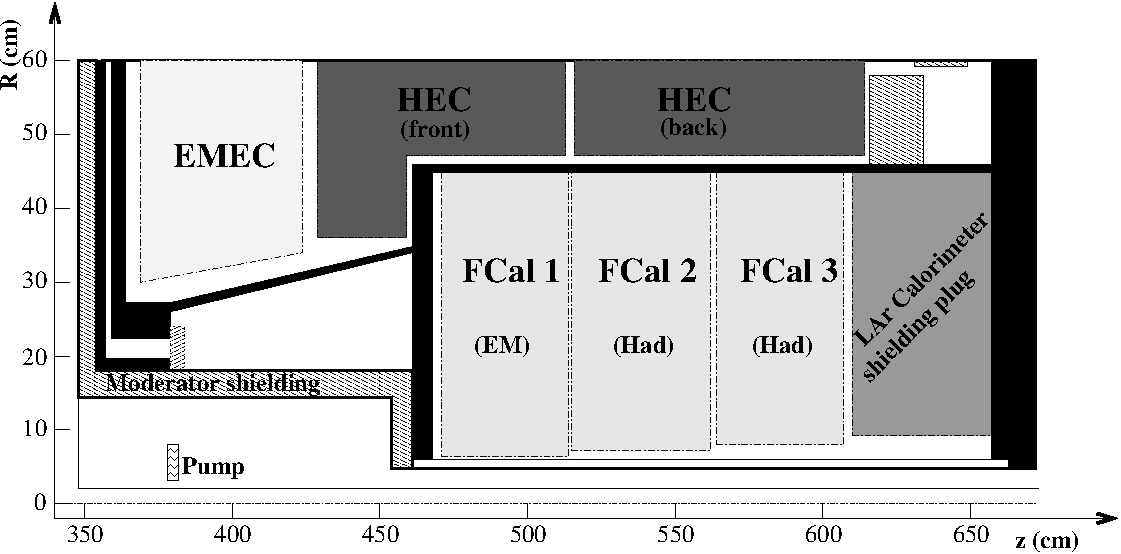
\includegraphics{figures/experiment/ATLAS_FCal_layout}}
	\caption{Schematic diagram showing the layout of the forward calorimeter in the $R$-$z$ plane.}
	\label{fig:ATLAS-calorimeters-fcal-layout}
\end{figure}


\begin{figure}
	\centering
	\subfloat[] {\label{fig:ATLAS-calorimeter-fcal1-electrodes}
		\resizebox{0.45\textwidth}{!}{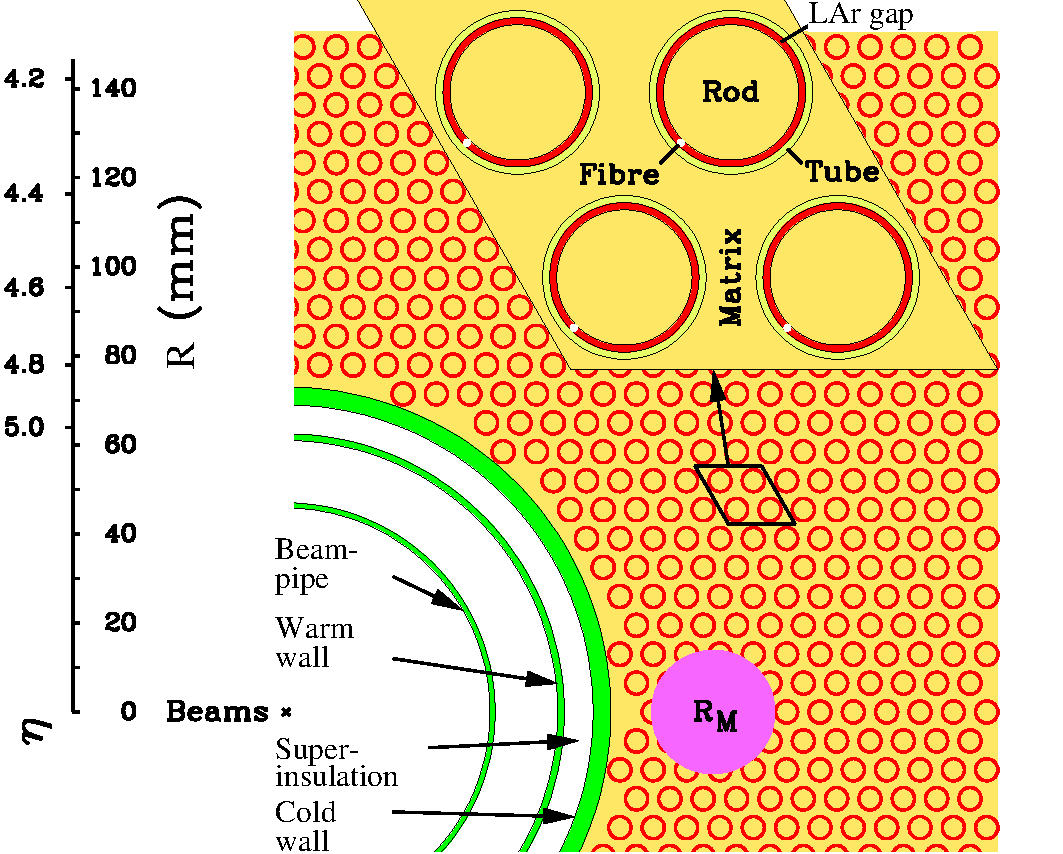
\includegraphics{figures/experiment/ATLAS_FCal1_electrodes}}
	}
	\hfill
	\subfloat[] {\label{fig:ATLAS-calorimeter-fcal23-electrodes}
		\resizebox{0.45\textwidth}{!}{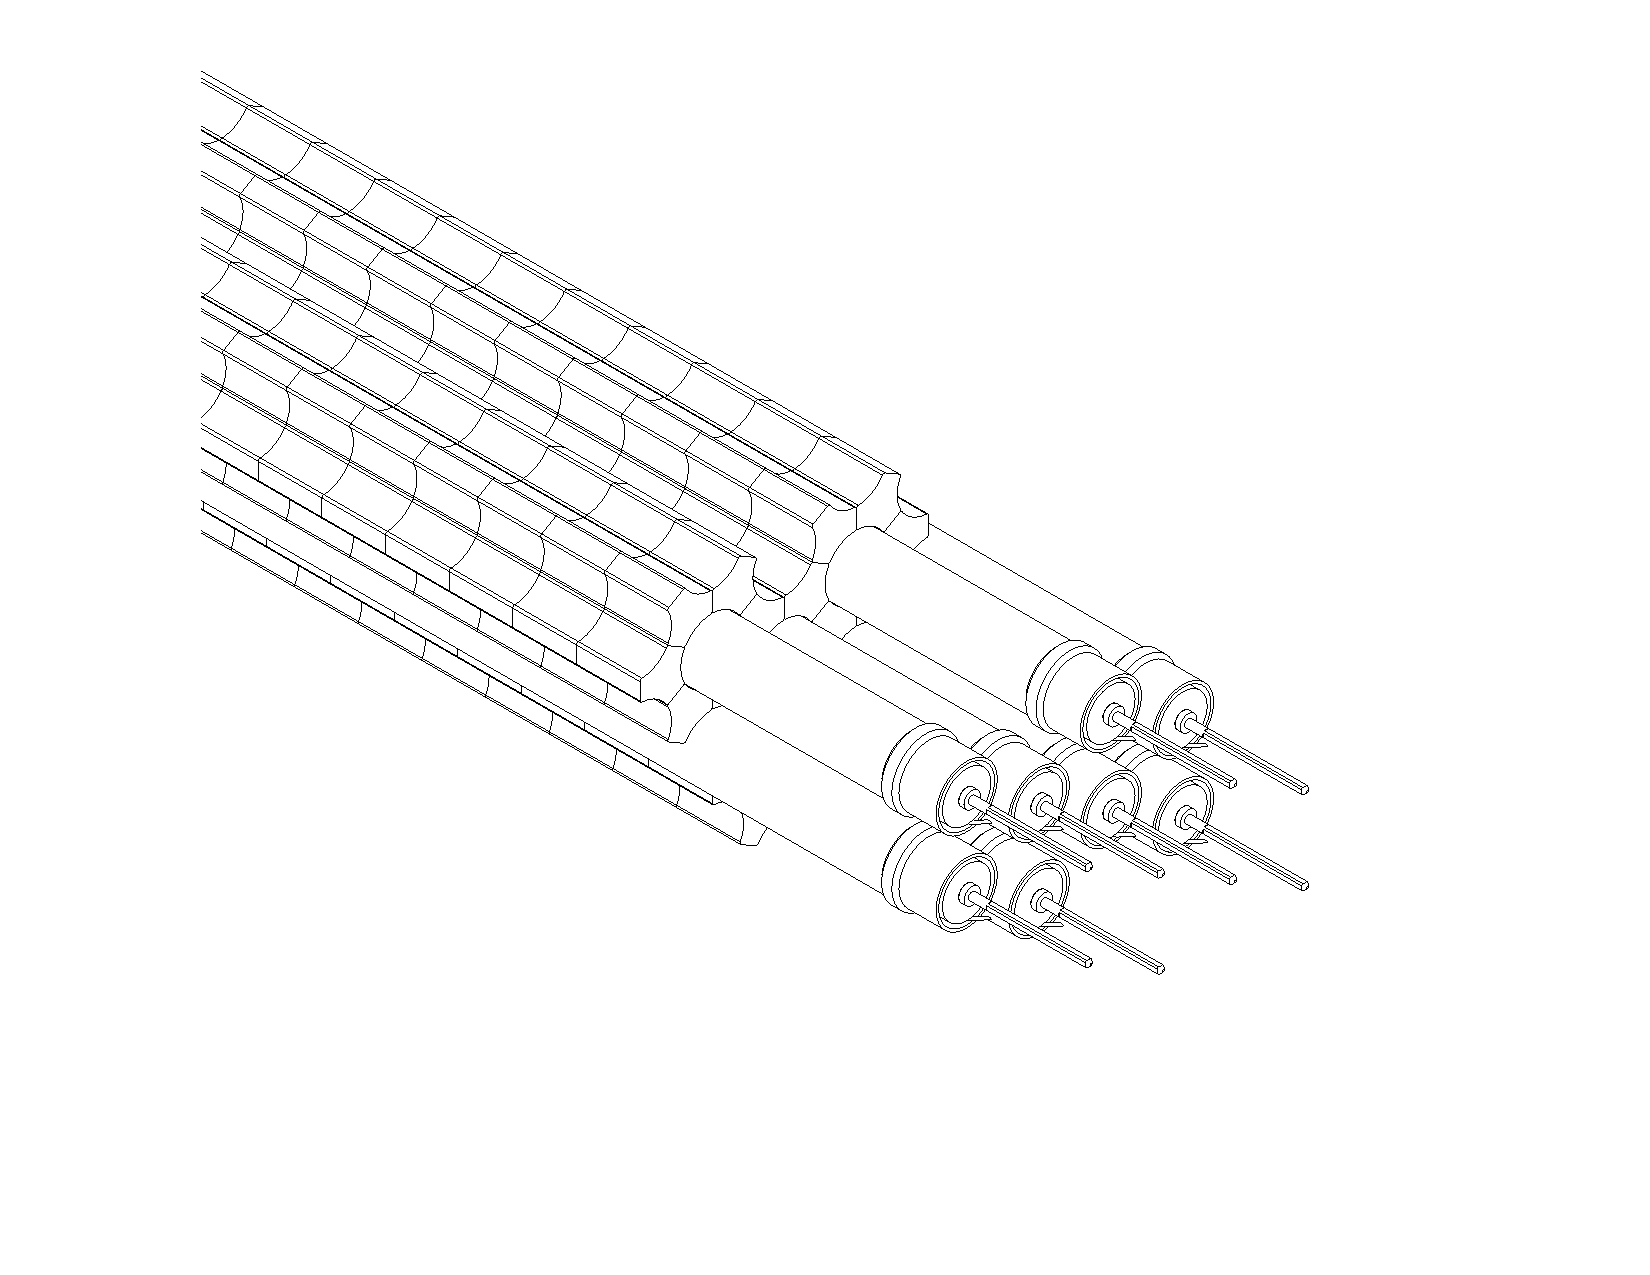
\includegraphics{figures/experiment/ATLAS_FCal23_electrodes_cropped}}
	}
	\caption{Left: the electrode structure of FCal1, showing the matrix of copper tubes and rods. The Moli{\`e}re radius, $R_{\mathrm{M}}$, is shown for reference. Right: the absorber matrix in FCal2 and FCal, made from tungsten rods and copper tubes.}
	\label{fig:ATLAS-calorimeter-fcal-electrodes}
\end{figure}


\subsection{Muon Spectrometer}\label{sec:ATLAS-muon-spectrometer}
The muon spectrometer detects charged particles that penetrate the barrel and end-cap calorimeters. It forms the exterior of the ATLAS detector, occupying the volume of the barrel toroid with four large wheels on each side of the interaction point. Using a combination of several technologies, the muon spectrometer performs precision measurements of muon momenta in the region $|\eta|<2.7$, with a design resolution of 10\% for $\SI{1}{\tera\electronvolt}$ tracks, and also provides triggering on muons for $|\eta|<2.4$. 

The structure of the muon spectrometer is shown in figures~\ref{fig:ATLAS-muon-spectrometer-layout} and \ref{fig:ATLAS-muon-spectrometer-schematic}. The barrel systems are arranged in three layers with radii of approximately $\SI{5}{\meter}$, $\SI{7.5}{\meter}$, and $\SI{10}{\meter}$, mounted inside and on the eight coils of the barrel toroid magnet with approximate octagonal symmetry. The end-cap systems form four large wheels, located before and after the end-cap toroid magnets at positions of $|z|\approx \SI{7.4}{\meter},\ \SI{10.8}{\meter},\ \SI{14}{\meter},$ and $\SI{21.5}{\meter}$. 

\begin{figure}[htbp]
	\centering
	\resizebox{0.6\textwidth}{!}{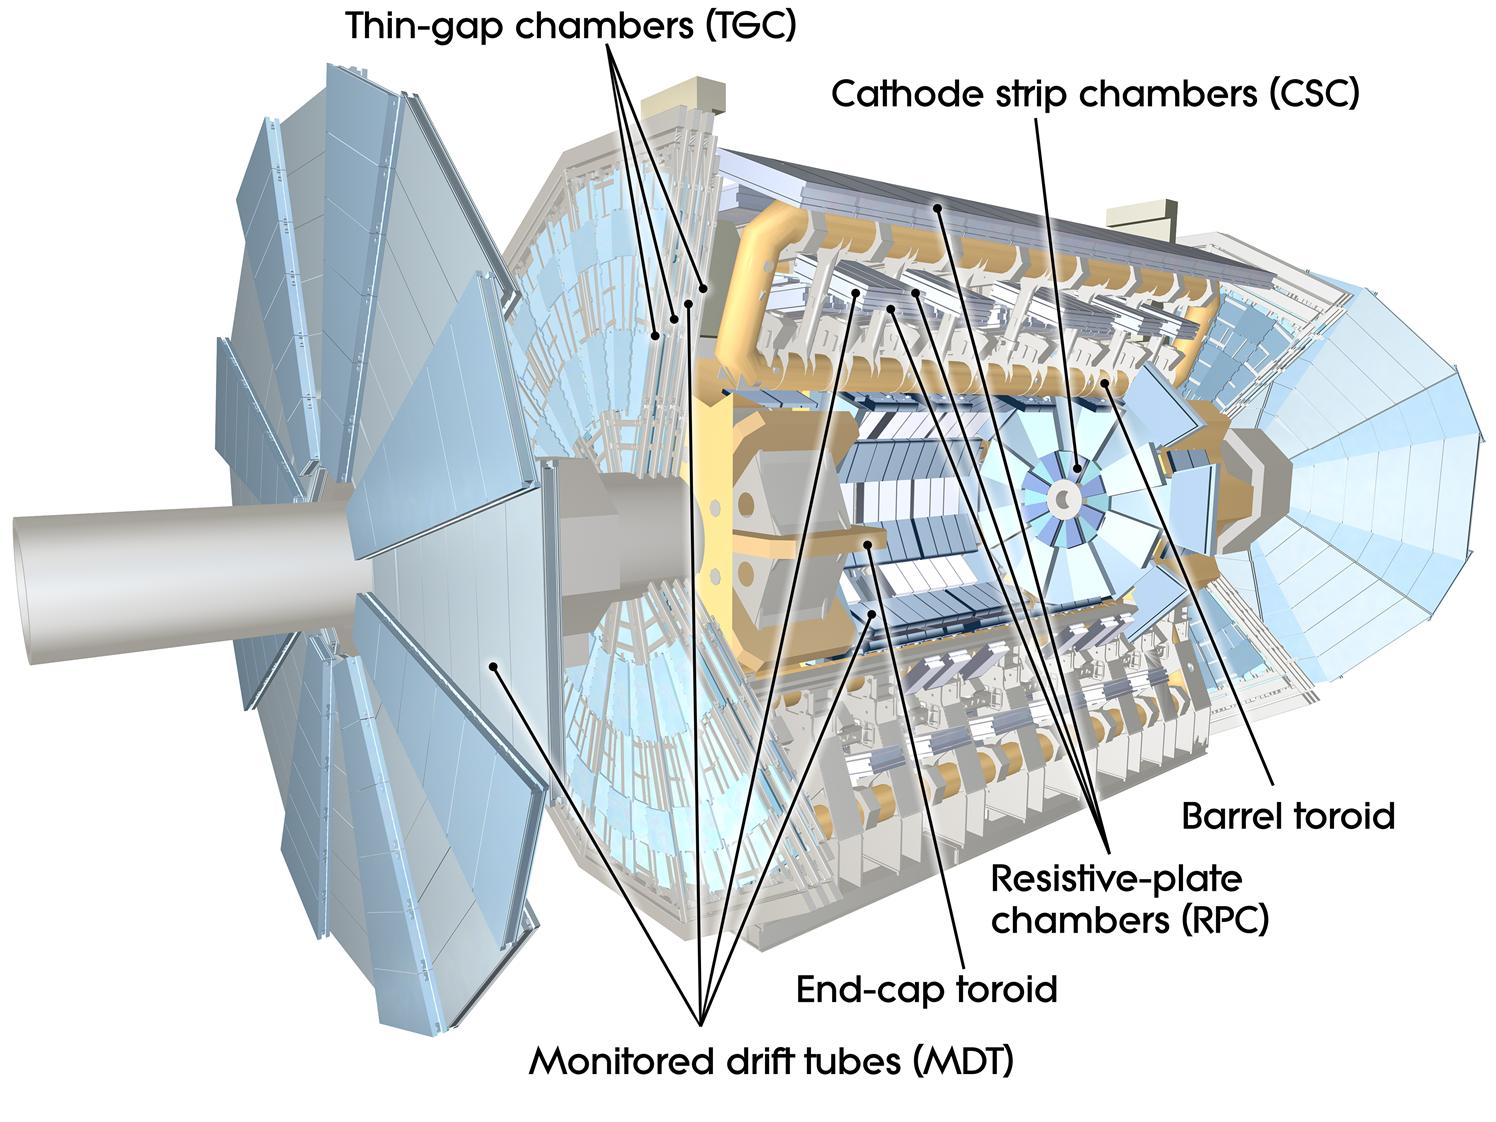
\includegraphics{figures/experiment/ATLAS_muons_sketch}}
	\caption{3D model of the ATLAS muon spectrometer. The four different types of detector (MDTs, CSCs, RPCs, and TGCs) and the toroid magnets are shown.}
	\label{fig:ATLAS-muon-spectrometer-layout}
\end{figure}

\begin{figure}[htbp]
	\centering
	\subfloat[ $R$-$z$ view of the muon spectrometer barrel. The barrel contains three layers, each with eight large and eight small chambers.] {
		\resizebox{0.45\textwidth}{!}{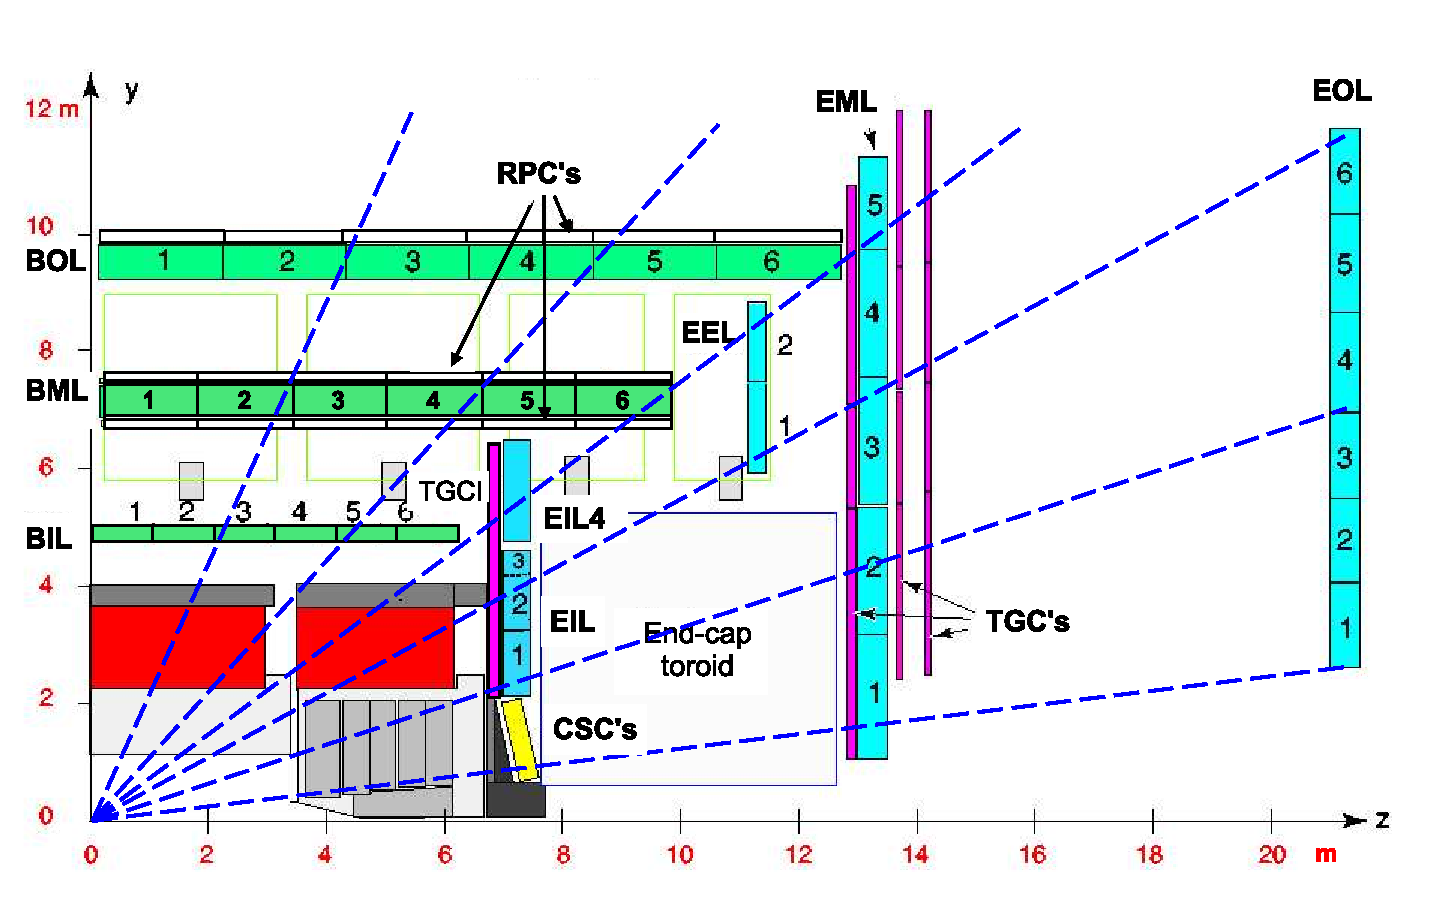
\includegraphics{figures/experiment/ATLAS_MS_layout_rz}}
	}
	\hfill
	\subfloat[ $R$-$\phi$ view of the muon spectrometer. The MDTs are shown in green and cyan, the CSCs in yellow, the TGCs in magenta, and the RPCs in white.] {
		\resizebox{0.45\textwidth}{!}{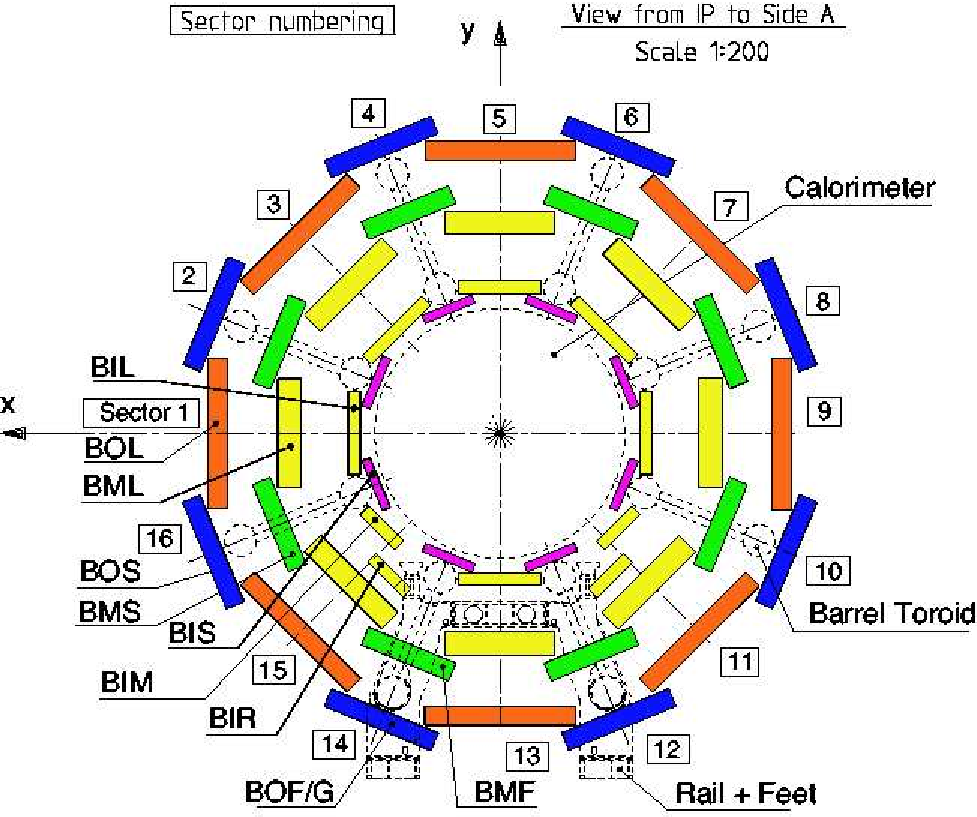
\includegraphics{figures/experiment/ATLAS_MS_layout_rphi}}
	}
	\caption{Layout of the chambers of the muon spectrometer.}
	\label{fig:ATLAS-muon-spectrometer-schematic}
\end{figure}



Four different technologies are used for precision measurements and triggering, depending on the location in the detector. Monitored drift tubes (MDTs) perform the precision measurements over most of the volume with $|\eta|<2.7$. Cathode strip chambers (CSCs) replace the MDTs in the innermost wheel for $2.0<|\eta|<2.7$, to handle the high particle flux. Triggering is performed by resistive plate chambers (RPCs) in the barrel ($|\eta|<1.05$) and thin gap chambers (TGCs) in the end-caps. The trigger chambers also supplement the MDT position measurements with the hit coordinate in the non-bending plane. 

\subsubsection{Monitored Drift Tubes}
The muon spectrometer contains 1088 MDT chambers, covering a total area of $\sim$\SI{550}{\meter\tothe{2}}. The majority of the MDT chambers are rectangular in the barrel and trapezoidal in the end-caps, and are laid out to optimize the solid angle coverage under the constraints of the magnet coils and other structures in the vicinity of the toroid magnet. Each chamber contains several layers of drift tubes, as shown in figure~\ref{fig:ATLAS-MS-MDT-chamber}. The innermost chambers are divided into two groups of tube layers, called \emph{multilayers}, each with four layers of tubes, while the remaining chambers have two groups of three layers of tubes. 

\begin{figure}[htbp]
	\centering
	\resizebox{0.6\textwidth}{!}{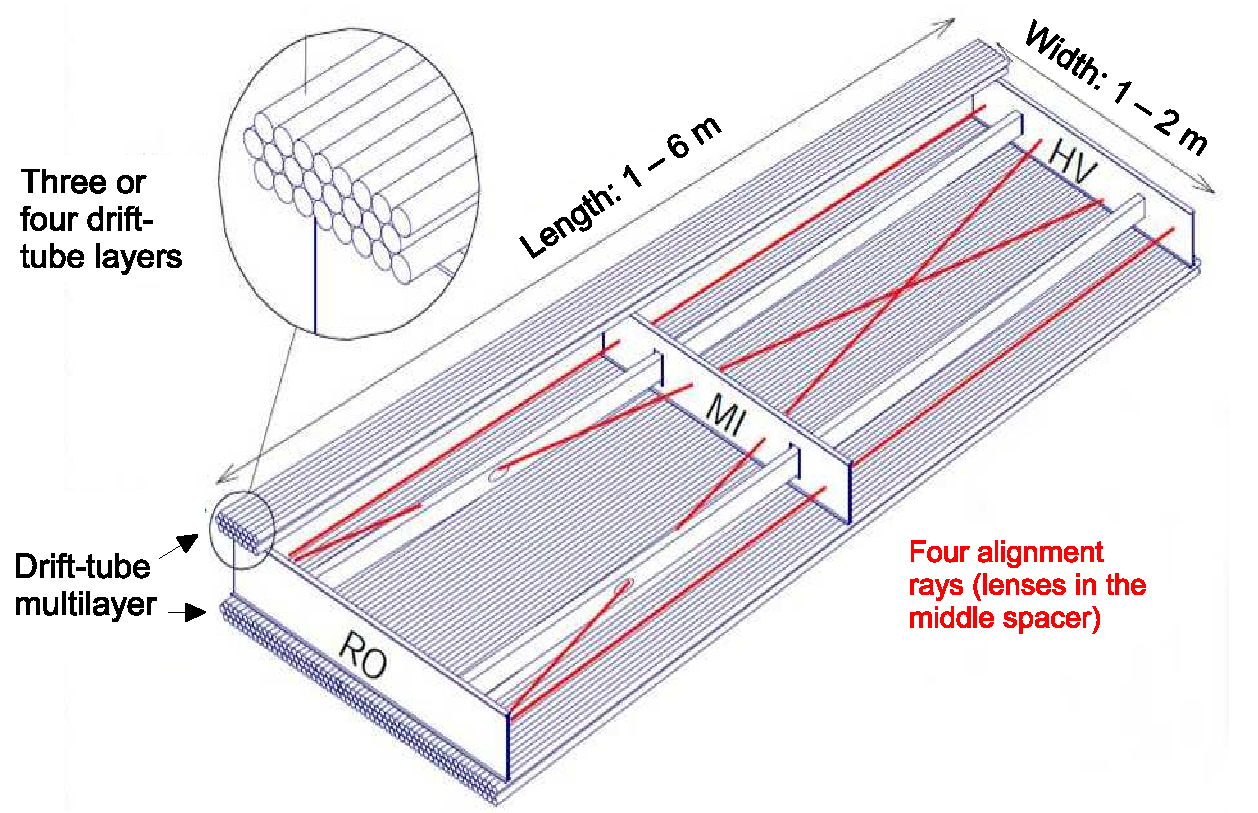
\includegraphics{figures/experiment/ATLAS_MDT_chamber}}
	\caption{The mechanical structure of a MDT chamber. Two multilayers, each consisting of three or four rows of drift tubes, are separated by aluminum spaceers. Four optical alignment rays continuously monitor the geometry of the chamber.}
	\label{fig:ATLAS-MS-MDT-chamber}
\end{figure}


The aluminum drift tubes have a radius of $\SI{29.97}{\milli\meter}$, with a $\SI{50}{\micro\meter}$-diameter tungsten-rhenium wire forming the anode along the axis of the tube. A cross section of a tube is shown in figure~\ref{fig:ATLAS-MS-MDT-xsec}. The tubes are filled with a mixture of argon and CO$_2$ (93:7) with a high pressure of $\SI{3}{\bar}$, and are operated with a voltage of $\SI{3080}{\volt}$. The average resolution of a single drift tube is $\SI{80}{\micro\meter}$, and the combined resolution of a chamber is $\SI{35}{\micro\meter}$. To achieve this precision, the position of the drift tubes and wires must be known to less than $\SI{30}{\micro\meter}$. Four optical alignment rays inside each MDT chamber continuously monitor the geometry of the chamber with a precision of a few microns, shown in figure~\ref{fig:ATLAS-MS-MDT-chamber}. An inter-chamber optical alignment network monitors the relative positions of chambers relative to their neighbors with a precision of approximately $\SI{20}{\micro\meter}$. The optical alignment is supplemented with track-based alignment algorithms to align the chambers with poor or absent connection to the optical network, the end-caps with respect to the barrel, and the muon spectrometer with respect to the inner detector.



%The operating voltage is $\SI{3080}{\volt}$, creating a radial electric field which allows for determination of the track position independent of the angle between the track and the tube. The tubes are filled with a mixture of argon and CO$_2$ (93:7) with a high pressure of 3~bar to reduce the impact of diffusion on the resolution. The gas mixture has good aging properties, but suffers from a long drift time, up to $\SI{700}{\nano\second}$ from the wall to the wire, and exhibits a nonlinear space-drift time relation which degrades the spatial resolution at high counting rates due to positive ions distorting the electric field. 

\begin{figure}[htbp]
	\centering
	\resizebox{0.4\textwidth}{!}{\includegraphics{figures/experiment/ATLAS_MDT_tube_cross_section}}
	\caption{Cross section of a drift tube, showing the cathode tube, the anode wire, and an illustration of a muon ionizing the gas as it traverses the tube.}
	\label{fig:ATLAS-MS-MDT-xsec}
\end{figure}

\subsubsection{Cathode Strip Chambers}
The rate limit for the safe operation of the MDTs is about \SI[per-mode=symbol]{150}{\hertz\per\centi\meter\tothe{2}}, which is exceeded for $|\eta|>2$ in the first layer of the end-cap at $|z|\approx \SI{7}{\meter}$. Accordingly, CSCs are used in this volume of the detector, which can operate up to rates of about \SI[per-mode=symbol]{1}{\kilo\hertz\per\centi\meter\tothe{2}}. Eight large and eight small trapezoidal chambers give full coverage in $\phi$, as shown in figure~\ref{fig:ATLAS-MS-CSC-layout}.  

The CSCs are multiwire proportional chambers, with parallel wires running in the radial direction and the two cathodes finely segmented in perpendicular directions to provide measurements in both the $\eta$ and $\phi$ directions. The perpendicular cathode segmentation provides position measurements in two dimensions, which helps distinguish hits from nearby particles. In the bending direction, the segmentation corresponds to a readout pitch of $\SI{5.31}{\milli\meter}$ and $\SI{5.56}{\milli\meter}$ for the large and small chambers, respectively.  The track coordinate is determined from a relative measurement of the charge induced on 3-5 adjacent strips at the peak of the charge distribution, shown schematically in figure~\ref{fig:ATLAS-MS-CSC-charge}. The resolution, dominated by electronic noise in the pre-amplifiers and by the spread of charge along the anode wire due inclined tracks, delta electrons, or a Lorentz force along the wire, is roughly $\SI{60}{\micro\meter}$ per CSC plane. In the non-bending direction, a coarser segmentation leads to a resolution of $\SI{5}{\milli\meter}$. 

\begin{figure}[htbp]
	\centering
	\subfloat[] {\label{fig:ATLAS-MS-CSC-layout}
		\resizebox{0.4\textwidth}{!}{\includegraphics{figures/experiment/ATLAS_CSC_geometry}}
	}
	\subfloat[] {\label{fig:ATLAS-MS-CSC-segmentation}
		\resizebox{0.4\textwidth}{!}{\includegraphics{figures/experiment/ATLAS_CSC_readout_strips2}}
	}
	\caption{Left: Layout of the eight large and eight small CSC chambers. Right: Schematic view of the CSC anode wires and perpendicular cathode strips, showing the deposition of charge from a track on several adjacent strips.}
	\label{fig:ATLAS-MS-CSC}
\end{figure}


\subsubsection{Resistive Plate Chambers}
Muon triggering in the barrel ($|\eta|<1.05$) is performed by 544 RPCs, which exhibit good spatial and timing resolution and an adequate rate capability of $\sim$\SI[per-mode=symbol]{1}{\kilo\hertz\per\centi\meter\tothe{2}}. The RPCs form three layers, or \emph{stations}, with two on either side of the middle MDT layer and the third on the inner or outer side of the outer MDT layer, for the small and large sectors, respectively. Each station has two independent layers, each providing a measurement of $\eta$ and $\phi$, resulting in six possible measurements for muons passing through three stations. 

An RPC unit consists of two sets of two parallel resistive plates ($\SI{2}{\milli\meter}$-thick phenolic-melaminic plastic laminate) separated by $\SI{2}{\milli\meter}$ by insulating spacers, shown in figure~\ref{fig:ATLAS-MS-RPC-schematic}. The interior is filled with a gas mixture of C$_2$H$_2$F$_4$/Iso-C$_4$H$_{10}$/SF$_6$ (94.7/5/0.3). With an electric field of $\SI[per-mode=symbol]{4.9}{\kilo\volt\per\milli\meter}$, muons traversing the gas induce an avalanche towards the anode, which is read out via capacitive coupling to $25$--$\SI{35}{\milli\meter}$-wide copper strips on the exterior face of the RPC. The RPCs achieve a spatial resolution of approximately $\SI{10}{\milli\meter}$ in $z$ and $\phi$, a timing resolution of $\SI{1.5}{\nano\second}$, and a detection efficiency of $\sim 98\%$. 

\begin{figure}[htbp]
	\centering
	\resizebox{0.6\textwidth}{!}{\includegraphics{figures/experiment/ATLAS_RPC_structure}}
	\caption{Cross section of an RPC, showing two units joined to form a single chamber. Each unit has two sets of two resistive plates (grey) separated by insulating spacers (green). The readout strips (magenta) are on the opposite side of the resistive plates from the gas gap. Outside the detecting elements, the volume of the RPC chamber is filled with paper honeycomb. The dimensions are given in millimeters.}
	\label{fig:ATLAS-MS-RPC-schematic}.
\end{figure}

\subsubsection{Thin Gap Chambers}
TGCs provide muon triggering in the end-caps, due to their good timing resolution and high rate capability. The TGCs also provide an azimuthal coordinate measurement, which complements the MDT measurement in the radial direction. Nine TGC disks are installed in total: a doublet mounted near the inner MDT end-cap layer, and a triplet and two doublets near the middle MDT end-cap layer. The disks are divided into two concentric annuli, one covering $1.05\leq |\eta| \leq 1.92$ and the other covering $1.92\leq|\eta|\leq2.4$. 

\begin{figure}[htbp]
	\centering
	\subfloat[ Cross sectional views of a TGC trilepton and a TGC doublet. The dimensions of the gas gaps are enlarged to show their structure.] {\label{fig:ATLAS-MS-TGC-triplet-doublet}
		\resizebox{0.5\textwidth}{!}{\includegraphics{figures/experiment/ATLAS_TGC_construction}}
	}
	\hfill
	\subfloat[ Closeup view of the TGC structure, showing the anode wires, graphite cathodes, and copper readout strips..] {\label{fig:ATLAS-MS-TGC-structure}
		\resizebox{0.4\textwidth}{!}{\includegraphics{figures/experiment/ATLAS_TGC_structure}}
	}
	\caption{The construction of the TGCs.}
	\label{fig:ATLAS-MS-TGC}
\end{figure}

The TGCs are multiwire proportional chambers filled with a gas mixture of CO$_2$ and $n$-pentane. The cathode planes are $\SI{1.6}{\milli\meter}$-thick FR4 (Flame Resistant 4) plates, with the interior faces coated with graphite and exterior faces cladded with copper. The triplet TGCs have three layers of wires and two layers of copper readout strips, while the doublet TGCs have two layers each of wires and strips, as shown in figure~\ref{fig:ATLAS-MS-TGC-triplet-doublet}. The radial coordinate is measured by the anode wire groups and the azimuthal coordinate by the radial cathode strips. The chambers are ``thin'' in that the wire to cathode distance, $\SI{1.4}{\milli\meter}$, is shorter than the wire-to-wire distance of $\SI{1.8}{\milli\meter}$, as shown in figure~\ref{fig:ATLAS-MS-TGC-structure}. The anode wires have a diameter of $\SI{50}{\micro\meter}$ and are operated at a potential of $\SI{2.9}{\kilo\volt}$. The small wire-to-wire distance and high electric field near the anode wires contribute to a good timing resolution of $\SI{4}{\nano\second}$. The spatial resolution, $2$--$\SI{6}{\milli\meter}$ in $R$ and $3$--$\SI{7}{\milli\meter}$ in $\phi$, is determined by the ganging of readouts: due to the direction of the magnetic field, achieving the required momentum resolution at fixed transverse momentum requires finer resolution at larger pseudorapidities. 


\subsection{Trigger and Data Acquisition}
During a typical data-taking run during 2012, the LHC beam contains 1377 bunches with a typical bunch spacing of $\SI{50}{\micro\second}$, giving an event rate of $\sim \SI{20}{\mega\hertz}$. In contrast, the ATLAS data acquisition system records events at roughly $\SI{400}{\hertz}$. The filtering of events is performed by the three-level ATLAS triggering system. The first level, L1, is implemented in hardware, and reduces the event rate to less than $\SI{75}{\kilo\hertz}$. The second level, L2, is implemented in software, and reduces the event rate to less than $\SI{3.5}{\kilo\hertz}$ using regions of interest (RoIs) identified by the L1 trigger. The final level of the trigger, the Event Filter, is also implemented in software, and reduce the event rate to less than $\SI{400}{\hertz}$ using the full event information. 

The L1 trigger reduces the event rate from $\SI{20}{\mega\hertz}$ to $\SI{75}{\kilo\hertz}$ using a limited subset of the event data. While the L1 trigger is processing an event, the full event data is stored in buffers on the detector. Due to the limited buffer size, the L1 latency must be less than $\SI{2.5}{\micro\second}$, of which $\SI{1}{\micro\second}$ is used by the cable propagation time. Therefore, the trigger is implemented in custom hardware processors. The block diagram for the trigger is shown in figure~\ref{fig:ATLAS-trigger-L1-block}. The inputs to the trigger include the RPC and TGC detectors in the muon spectrometer and all of the calorimeter system.  Two primary systems, the L1 Calorimeter Trigger and the L1 Muon Trigger, select events based on the presence of high-$\Et$ objects or significant total event activity. These include high-$\pt$ muons, electron and photons, jets, hadronically decaying tau leptons, large missing transverse energy, and large total transverse energy. 

\begin{figure}[htbp]
	\centering
	\resizebox{0.4\textwidth}{!}{\includegraphics{figures/experiment/ATLAS_trigger_L1_block2}}
	\caption{Block diagram of the L1 trigger system.}
	\label{fig:ATLAS-trigger-L1-block}
\end{figure}

The L1 Calorimeter Trigger uses about 7,000 analogue trigger towers with a reduced granularity, $\Delta\eta\times\Delta\phi=0.1\times0.1$ for most of the detector. Two subsystems run in parallel: the cluster processor identifies electrons/photons and hadronically decay tau lepton candidates with $\Et$ above a programmable set of thresholds, while the jet/energy-sum processor identifies jets and calculates the total scalar transverse energy and $\Etmiss$ using $\Delta\eta\times\Delta\phi=0.2\times0.2$ blocks of calorimeter cells. Isolation cuts can be applied as well, limiting the energy allowed in the towers surrounding the object of interest and, in the case of electrons/photons, in the hadronic towers behind the electromagnetic towers. 

The L1 Muon Trigger searches for a coincidence of hits in consecutive muon trigger stations within a \emph{road}, roughly corresponding to the path of a muon from the interaction point through the detector. The $\pt$ threshold is encoded in the width of the road, with a narrower road corresponding to a higher $\pt$ threshold. For low-$\pt$ muons in the RPCs, the algorithm begins with hits in the second RPC doublet, called the \emph{pivot plane}. The trigger requires a hit in the first RPC doublet, within the road defined by the interaction point and the hit in the pivot plane. The high-$\pt$ algorithm is similar, requiring a hit along the road in the third RPC doublet as well as the first two.In the end-caps, the pivot plane is established by the outermost layer of TGCs, with the road corresponding to the path of an infinite-momentum muon originating from the interaction point. To reject backgrounds from random coincidences, stricter requirements are imposed on the number of coincident hits in the TGC doublets and triplets.

The muon and calorimeter triggers pass their decisions along with the corresponding data to the Central Trigger Processor (CTP). The CTP communicates the total trigger decision to the front ends on the detector, including special triggers such as random triggers or the minimum bias trigger based on scintillator counters. In the event of a passed trigger, the event data is passed to the L2 trigger. The CTP also manages the \emph{luminosity blocks}, an index representing the time at which an event was recorded with coarse ($\sim1$ minutes) granularity. A luminosity block is the shortest time interval for which the integrated luminosity can be determined such that the total uncertainty is dominated by systematic effects, rather than limited statistics. In the event of a detector failure, this index allows the rejection of a minimal set of affected events. 

The L2 trigger reduces the event rate from a maximum of $75~\mbox{kHz}$ from the L1 trigger to less than $\SI{3.5}{\kilo\hertz}$. The trigger is implemented in software, and uses only the subset of the event data within the RoIs identified by the L1 trigger, typially $1\%$-$2\%$ of the total. After a successful L1 trigger, the data corresponding to the RoIs, stored in the detector-specific front end electronics, are accumulated in the RoI builder via 1574 readout links. The RoI builder combines the 1574 event fragments into a single data structure, which is passed to the L2 processing farm. At each step of a given trigger algorithm targeting particular signatures, only the relevant RoIs are analyzed. If no signatures remain valid, the event is rejected. Hence the full RoI information is transferred only for events which pass the L2 selection criteria. The typical L2 latency is about $\SI{40}{\milli\second}$.

Finally, the event filter reduces the event rate to the final $\sim$\SI{400}{\hertz} read out from the detector to disk. Also implemented in software, it runs the same algorithms as used in the offline event reconstruction using the full event information. Based on the objects used for triggering, the triggered events are categorized into one or more \emph{data streams}. The data streams and other data computed by the event filter are appended to the event data, which are then transferred to CERN’s central data-recording facility for storage. An example of the event filter rates from the various streams during a single data-taking run is shown in figure~\ref{fig:ATLAS-trigger-EF-rates-singlerun}. The monthly average rates of each stream during 2012 are shown in figure~\ref{fig:ATLAS-trigger-EF-rates-2012}.

\begin{table}[htbp]
	\centering
	\subfloat[ Event filter rates for a single data-taking run.] {\label{fig:ATLAS-trigger-EF-rates-singlerun}
		\resizebox{0.4\textwidth}{!}{\includegraphics{figures/experiment/ATLAS_trigger_streamrates_singlerun.eps}}
	}
	\hfill
	\subfloat[ Average monthly event filter rates during 2012.] {\label{fig:ATLAS-trigger-EF-rates-2012}
		\resizebox{0.55\textwidth}{!}{\includegraphics{figures/experiment/ATLAS_trigger_streamrates_2012}}
	}
	\caption{The rates of recording events from the event filter for different data streams.}
	\label{fig:ATLAS-trigger-EF-rates}
\end{table}


\printbibliography
\chapter{Luminosity Measurement}\label{ch:luminosity}
\section{Run I Luminosity}

The ATLAS Run I data were recorded from 2011 to 2012, with a center-of-mass collision energy of $\sqrt{s}=\SI{7}{\tera\electronvolt}$ in 2011 and $\sqrt{s}=\SI{8}{\tera\electronvolt}$ during 2012. Integrated luminosities of $L=\SI{5.46}{\femto\barn\tothe{-1}}$ and $\SI{22.8}{\femto\barn\tothe{-1}}$ were delivered by the LHC in the two years, of which $\SI{5.08}{\femto\barn\tothe{-1}}$ and $\SI{21.3}{\femto\barn\tothe{-1}}$ were recorded by the ATLAS detector. The recorded luminosity accounts for the data acquisition inefficiency, as well as the warm start period, an interval of several minutes after the LHC has declared stable beams during which the tracking detectors are ramped to high voltage and the pixel detector preamplifiers are turned on. After masking data recorded while one or more detector subsystems were not functioning properly, $\SI{4.57}{\femto\barn\tothe{-1}}$ and $\SI{20.3}{\femto\barn\tothe{-1}}$ of data are considered usable for physics analyses. The volume of delivered, recorded, and physics-ready data are shown as a function of time in figure~\ref{fig:luminosity-runI}. 

The LHC was typically operated with 1042 and 1368 colliding bunches in 2011 and 2012, respectively, with a bunch spacing of $\SI{50}{\nano\second}$. The peak instantaneous luminosity reached values as high as $\mathcal{L}\sim\SI[per-mode=symbol]{8e33}{\centi\meter\tothe{-2}\second\tothe{-1}}$, corresponding to a peak average pileup value of $\mu\sim37$. The distribution of pileup values in 2011 and 2012 data are shown in figure~\ref{fig:luminosity-pileup}. 

\begin{figure}[htbp]
	\centering
	\hfill
	\subfloat[] {\label{fig:luminosity-runI}
		\resizebox{0.45\textwidth}{!}{\includegraphics{figures/reconstruction/intlumivstime2011-2012DQ.eps}}
	}
	\hfill
	\subfloat[] {\label{fig:luminosity-pileup}
		\resizebox{0.45\textwidth}{!}{\includegraphics{figures/reconstruction/mu_2011_2012-dec.eps}}
	}
	\hfill
	\caption{Left: The cumulative delivered, recorded, and physics-ready integrated luminosity versus time in 2011-2011. Right: Distribution of the number of interactions per bunch crossing in events recorded in 2011-2012.}
	
\end{figure}


% New section?

\section{Measurement Overview}\label{sec:luminosity-overview}
The instantaneous luminosity at a $pp$ collider is given by~\cite{Grafstrom:2015go,Aad:2013ucp}:

\begin{equation}
	\mathcal{L} = \frac{R_{\mathrm{inel}}}{\sigma_{\mathrm{inel}}},
\end{equation}

where $R_{\mathrm{inel}}$ is the rate of inelastic $pp$ collisions, and $\sigma_{\mathrm{inel}}$ is the $pp$ inelastic cross section. For a storage ring with a revolution frequency $f_r$ and $n_b$ colliding bunch pairs, the instantaneous luminosity can be written in terms of the average number of inelastic $pp$ collisions per bunch crossing, $\mu$, as 

\begin{equation}
	\mathcal{L} = \frac{\mu f_r n_b}{\sigma_{\mathrm{inel}}}.
\end{equation}

The instantaneous luminosity is measured by ATLAS using several detectors and algorithms, which have some efficiency $\epsilon$ to detect a $pp$ interaction and measure the \emph{visible} number of interactions per bunch crossing, $\mu_{\mathrm{vis}} = \epsilon \mu$. Defining the visible cross section to be $\sigma_{\mathrm{vis}}\equiv \epsilon \sigma_{\mathrm{vis}}$, the instantaneous luminosity as measured by a particular detector is:

\begin{equation}\label{eqn:luminosity-detected}
	\mathcal{L} = \frac{\mu_{\mathrm{vis}} f_r n_b}{\sigma_{\mathrm{vis}}}.
\end{equation}

The instantaneous luminosity is measured in intervals of approximately 60~seconds. The visible cross section is a calibration constant for a particular detector, which is determined during dedicated calibration runs in which the luminosity is determined directly from the physical dimensions of the beams. The calibration procedure is described in section~\ref{sec:luminosity-calibration}. 

\section{Luminosity Detectors}\label{sec:luminosity-detectors}
ATLAS performs many redundant luminosity measurements using several detectors. The detectors fall into two categories. \emph{Event counting} detectors have a binary response, returning a 0 or 1 depending on whether a bunch crossing satisfies a set of criteria defined to detect an inelastic $pp$ collision. Such detectors essentially measure $p(0;\,\mu)$, the probability that an event falls in the zero bin of a Poisson distribution, from which the mean $\mu$ be calculated. \emph{Hit counting} detectors, on the other hand, count some quantity proportional to the number of interactions in a given bunch crossing, such as the number of particles identified by a particular detector subsystem. A hit counting measurement typically yields more information about an event at the cost of additional systematic uncertainties.

Ideally, a luminosity detector exhibits the following features: 

\begin{itemize}
	\item The efficiency of the detector should be insensitive to pileup. The visible cross sections are typically measured at $\mu\approx \mathcal{O}(1)$, while a typical data-taking run has a peak average pileup of up to $\mu\sim40$; it is essential that the visible cross section be constant across this range of pileup values.

	\item The efficiency of the detector should also be constant over long timescales.

	\item The response of the detector and the readout should fast enough to provide a bunch-by-bunch luminosity measurement. As the LHC bunches are not identical, with different numbers of protons and emittances, it is useful to measure luminosity for each colliding bunch pair, as often as once every $\SI{25}{\nano\second}$. The colliding bunch pairs are labeled by the bunch crossing identification number, or BCID, ranging from 1 to 2808; consecutive BCIDs are separated by $\SI{25}{\nano\second}$.

	\item The efficiency should be high enough to yield sufficient statistics. The data are used in increments as shorts as $\SI{20}{\second}$, so the statistics collected over this time scale scale should be high enough that the total uncertainty is dominated by systematic effects. On the other hand, for event counting detectors, the efficiency should not be so high that the detector is saturated; the uncertainty on $\mu$ is large if $p(0;\mu)$ is too close to 0 or 1. 

	\item The backgrounds should be low and understandable. Detectors can be sensitive to a wide range of phenomena aside from $pp$ collisions, which should not be counted as luminosity. For example, some detectors observe a phenomenon called \emph{afterglow}, a small amount of activity in the BCIDs immediately following a collision likely due to photons from nuclear deexcitations in the detector material. The afterglow background is proportional to the luminosity in the colliding BCIDs, and decays away with several time constants. Collisions between a beam and residual gas in the beam pipe, called \emph{beam-gas interactions}, can also contribute a low level of background, and is estimated by observing non-colliding bunches passing through the interaction region.

\end{itemize}

The central value of the luminosity measurement is determined by the \emph{beam conditions monitor} (BCM)~\cite{Cindro:2008zz}, which fulfills most of these desired criteria. The BCM consists of eight diamond-based particle detectors, four on each side of the interaction point at $|z|=\SI{184}{\centi\meter}$ and $|\eta|=4.2$. The detectors are have a physical cross section of approximately $\SI{1}{\centi\meter\tothe{2}}$ and are arranged in a cross pattern, with two independent readouts corresponding to the vertical and horizontal pairs. The design purpose of the BCM is to monitor backgrounds and to trigger a beam dump if beam losses towards the inner detector become too high; accordingly, the detector has a very fast readout, and can provide a bunch-by-bunch luminosity measurement with a time resolution of $\sim \SI{0.7}{\nano\second}$. The luminosity is measured using event counting, and can be measured using any combination of the readouts. The configurations used require hits in either the vertical pair (BCMV) or the horizontal pair (BCMH), and either coincident hits on both sides of the interaction point (AND) or a single hit on either side (OR). The small size of the active sensor leads to an efficiency of approximately 7\% in the OR configuration, which allows for sufficient statistics without saturating the detector. 

LUCID (LUminosity measurement using Cherenkov Integrating Detector)~\cite{TheATLASCollaboration:2008fg} provides a supplementary, bunch-by-bunch, event counting-based luminosity measurement. The detector consists of two sets of sixteen Cherenkov detectors surrounding the beampipe at $z=\pm\SI{17}{\meter}$, occupying the pseudorapidity range $5.6<|\eta|<6.0$. As designed and initially constructed, the Cherenkov detectors are polished aluminum tubes filled with C$_4$F$_{10}$ gas. The Cherekov photons induced by charged particles traversing the gas are collected by photomultiplier tubes (PMTs) located at the far end of the tubes. Additional Cherenkov photons are produced in the quartz window separating the tube volume from the PMT. In this configuration, the typical single-particle yield is 60-70 photoelectrons due to photons created in the gas, and about 40 photoelectrons due to the quartz window. A hit is recorded if the PMT signal exceeds a preset threshold, corresponding to about 15 photoelectrons. However, the higher instantaneous luminosities due to the $\SI{50}{\nano\second}$ bunch spacing led to saturation of the detectors, and hence on 30 July 2011, the gas was removed from the Cherenkov tubes to reduce the efficiency. The removal of the gas also improved the detector's stability and linearity with respect to pileup. Relative comparisons with other detectors were used to reestablish the detector calibration.

Several detector subsystems nominally designed for physics object reconstruction are also used for hit counting-based luminosity measurements. Algorithms using the tile calorimeter and the forward calorimeters (see section~\ref{sec:ATLAS-calorimeters}) determine the luminosity from detector currents proportional to the total particle flux in small regions of the calorimeters. The tile calorimeter algorithm monitors the PMT currents corresponding to a few selected cells near $|\eta|=1.25$, where the highest sensitivity to changes in the luminosity is observed. Similarly, the forward calorimeter algorithm monitors the currents in the high voltage lines. In both cases, the detector is unable to provide a bunch-by-bunch measurement, and the current response is not sensitive to the low instantaneous luminosities during the dedicated calibration runs, requiring the calibration to be set using relative comparisons with LUCID or BCM. On the other hand, the detectors exhibit good linearity of response with pileup, and good short-term stability. 

Finally, algorithms using the inner detector measure the luminosity by counting reconstructed tracks and vertices\footnote{Pixel cluster counting, used by the CMS experiment, was also considered, but was not commissioned due to the difficulty of the subtraction of the background due to afterglow.}. The use of these higher-level objects confers certain benefits, such as low background rates and good long-term stability, at the cost of increased computational requirements, which limit the data rate to $\mathcal{O}(\SI{100}{\hertz})$. Further, pileup effects can be significant; in particular, the efficiency of the vertex counting algorithm varies by as much as $30\%$ up to pileup values of $\mu=30$, limiting its utility to data with low pileup. 

\section{Luminosity Calibration: van der Meer Scans}\label{sec:luminosity-calibration}
The visible cross sections for the detectors and algorithms described in section~\ref{sec:luminosity-detectors} are calibrated during dedicated runs called van der Meer (vdM) scans~\cite{vanderMeer:1968ud}. The calibration procedure uses the definition of luminosity in terms of the beam parameters, given for a single colliding bunch by:

\begin{equation}\label{eqn:luminosity-geometrical}
	\mathcal{L} = f_r n_1 n_2 K \int \rho_1(x,y,z,t) \rho_2(x,y,z,t)\, dx\,dy\,dz\,dt,
\end{equation}

where $f_r$ is the revolution frequency, $n_{1,2}$ are the number of particles in the colliding bunches, and $\rho_{1,2}(x,y,z,t)$ are the time- and position-dependent particle density distribution, normalized so that $\int \rho_{1,2}(x,y,z,t)\,dx\,dy\,dz = 1$. $K$ is a kinematic factor,

\begin{equation}
	K=\sqrt{(\vec{v}_1-\vec{v}_2)^2 - \frac{(\vec{v}_1\times\vec{v}_2)^2}{c^2}},
\end{equation}

which, in the limit $|\vec{v}_{1,2}|\rightarrow c$, reduces to $2c\cos\alpha$, where $\alpha$ is the crossing angle between the beams. To simplify the current discussion, the crossing angle is assumed to be zero, and the bunch densities are assumed to be functions of $x$, $y$, and $z\pm ct$, i.e. that the transverse bunch profiles are constant over the duration of the collision\footnote{In particular, the \emph{hourglass effect} is neglected. The collisions occur in a drift space, where the beams are focused, or squeezed, onto the interaction point. The transverse size of the beam in direction $i$ as a function of $z$ is given by $\sigma_{i}^2(z)=\epsilon_{i} \beta^*_{i} \left(1+\frac{(z-z_{i}^w)^2}{{\beta^*_{i}}^2}\right)$, where $\epsilon_{i}$ is the transverse emittance, $z_i^w$ is location of the optical waist, and $\beta^*_i$ is the betatron function at $z=z_i^w$. The effect is significant when $\beta^*_i\lesssim \sigma_z$; during the vdM scans, $\sigma_z\approx \SI{50}{\milli\meter}$, while $\beta^*=\SI{1.5}{\meter}$-$\SI{11}{\meter}$, and hence the hourglass effect is neglected.}. The luminosity can then be expressed as:

\begin{equation}
	\mathcal{L}=f_r n_1 n_2 \int \hat{\rho}_1(x,\,y)\hat{\rho}_2(x,\,y)\, dx\,dy,
\end{equation}

where $\hat{\rho}_{1,2}(x,\,y)$ are the transverse particle densities, normalized to unity. Under the further assumption that the transverse particle densities factorize in the horizontal and vertical directions, $\hat{\rho}(x,\,y)=\hat{\rho}_x(x)\hat{\rho}_y(y)$, where $\hat{\rho}_x(x)$ and $\hat{\rho}_y(y)$ are also normalized to unity, the luminosity can be written as:

\begin{equation}
	\mathcal{L} = f_r n_1 n_2 \Omega_x(\hat{\rho}_{x1},\,\hat{\rho}_{x2}) \Omega_y(\hat{\rho}_{y1},\,\hat{\rho}_{y2}),
\end{equation}

where $\Omega_x(\hat{\rho}_{x1},\,\hat{\rho}_{x2})=\int \hat{\rho}_{x1}(x) \hat{\rho}_{x2}(x) dx$, and similarly for the $y$ direction\footnote{The formalism can be generalized to the case where the beam profiles do not factorize in $x$ and $y$; see~\cite{Balagura:2011er}.}. As first proposed by van der Meer, the $\Omega_{x,y}$ parameters can be determined by measuring the interaction rate as a function of transverse beam displacement, $R_{x,y}(\delta)$. Without loss of generality, assume that beam 2 is displaced by $\delta$ in the $x$ direction, while beam 1 is held fixed. Then, $R_{x}(\delta) = k \int \rho_{x1}(x) \rho_{x2}(x-\delta)\, dx$ for some constant $k$, and 

\begin{align}
	\frac{R_x(0)}{\int R_x(\delta) d\delta} &= \frac{k\int \rho_{x1}(x) \rho_{x2}(x)\, dx}{k\int\int \rho_{x1}(x)\rho_{x2}(x-\delta) \, dx\, d\delta} \\
	&= \int \rho_{x1}(x)\rho_{x2}(x)\, dx \\
	&= \Omega_x (\hat{\rho}_{x1},\,\hat{\rho}_{x2})
\end{align}

For convenience, define $\Sigma_{x,y}$ to be the characteristic widths of $R_{x,y}(\delta)$, given by:

\begin{equation}\label{eqn:luminosity-CapSigma}
	\Sigma_{x,y}=\frac{1}{\sqrt{2\pi}} \frac{\int R_{x,y}(\delta)\,d\delta}{R_{x,y}(0)}.
\end{equation}

For Gaussian beams, $\Sigma_{x,y}$ correspond to the Gaussian width of $R_{x,y}(\delta)$. Finally, the luminosity is given by

\begin{equation}
	\mathcal{L} = \frac{f_r n_1 n_2}{2\pi \Sigma_x \Sigma_y}.
\end{equation}

Equating this with the luminosity defined in equation~\ref{eqn:luminosity-detected}, the visible cross section for a given detector and algorithm is given by

\begin{equation}
	\sigma_{\mathrm{vis}} = \mu_{\mathrm{vis}}^{\mathrm{MAX}} \frac{2\pi \Sigma_x \Sigma_y}{n_1 n_2},
\end{equation}

where $\mu_{\mathrm{vis}}^{\mathrm{MAX}}$ is the visible interaction rate per bunch crossing at the maximum of the scan curve, $R(\delta)$. The numbers of particles per bunch, $n_{1,2}$, are measured by the LHC Bunch Current Normalization Working Group using bunch current transformers (BCTs)~\cite{Barschel:1425904,Anders:1427726,Alici:1427728}. 

\subsection{2011 Luminosity Calibration}

As an example, the 2011 $pp$ calibration is derived from two pairs of scans in the $x$- and $y$-directions, performed during the same LHC fill on 15 May 2011~\cite{Aad:2013ucp}. The beams had 14 colliding bunch pairs, $\sim0.8\times 10^{11}$ protons per bunch, $\beta^*=\SI{1.5}{\meter}$, and a crossing angle of $\alpha=\SI{240}{\micro\radian}$. The resulting transverse beam size was approximately $\sigma_{x}\approx\sigma_{y}\approx \SI{40}{\micro\meter}$, and the peak average number of interactions per crossing with head-on collisions was $\mu\approx 2.3$. The scan was performed in 25 equal steps over a displacement range of $\delta=\pm 233 \micron$.

Figure~\ref{fig:vdm-curve} shows an example scan curve, with the specific visible interaction rate, $\mu_{\mathrm{vis}}^{\mathrm{sp}}\equiv \mu_{\mathrm{vis}}/(n_1n_2)$, plotted as a function of transverse beam separation for the BCMV\_OR algorithm. Normalizing by the bunch current product, $n_1n_2$, eliminates the dependence of the curve on the decreasing beam currents over the course of the scan. The vdM scan curve is fitted with a Gaussian plus a constant, which is used as $R_{x,y}(\delta)$ to calculate $\Sigma_{x,y}$ in equation~\ref{eqn:luminosity-CapSigma}. $\mu_{\mathrm{vis}}^{\mathrm{MAX}}$ is determined from the peak of the fitted function. The measured $\sigma_{\mathrm{vis}}$ values for both scans and all 14 colliding bunch pairs are shown in figure~\ref{fig:vdm-sigmavis-bcm-2011}. The luminosity-weighted mean $\sigma_{\mathrm{vis}}$ is taken as the central value, while the scatter of the 28 measurements, which is not consistent with statistical variation, is taken as a systematic uncertainty on the reproducibility of the measurement. 

The visible cross sections for several algorithms using during 2011 are shown in table~\ref{table:luminosity-sigmavis-summary}, along with the efficiency assuming a total inelastic cross section of $\sigma_{\mathrm{inel}}= \SI{71.34\pm0.9}{\milli\barn}$~\cite{TheATLASCollaboration:2014jo}.

\begin{figure}[htbp]
	\centering
	\resizebox{0.6\textwidth}{!}{\includegraphics{figures/luminosity/VDM_BCMVOR_example}}
	\caption{An example of a scan curve measured by BCMV\_OR from the van der Meer scans on 15 May 2011. The specific visible interaction rate $\mu_{\mathrm{vis}}^{\mathrm{sp}}\equiv \mu_{\mathrm{vis}}/(n_1n_2)$ is shown as a function of transverse beam separation in the $x$ direction for a single scan and BCID. The data are fitted with Gaussian plus constant. The bottom plot shows the residual deviation of the data from the fit, divided by the uncertainty on the data.}
	\label{fig:vdm-curve}
\end{figure}

\begin{figure}[htbp]
	\centering
	\resizebox{0.6\textwidth}{!}{\includegraphics{figures/luminosity/VDM_sigmavis_BCMVOR}}
	\caption{Measured $\sigma_{\mathrm{vis}}$ values from the vdM scans performed in May 2011. The error bars represent statistical uncertainties only. The vertical dashed lines indicate the weighted average over BCIDs from the two sets of scans. The yellow band shows a variation of $\pm0.9\%$ from the total weighted average, equal to the systematic uncertainty due to the observed BCID-to-BCID and scan-to-scan variations.}
	\label{fig:vdm-sigmavis-bcm-2011}
\end{figure}


\begin{table}[htbp]
	\centering
	\begin{tabular}{|l|c|c|}
		\hline
		Algorithm & $\sigma_{\mathrm{vis}}$ (2011) & $\frac{\sigma_{\mathrm{vis}}}{\sigma_{\mathrm{inel}}}$ \\
		\hline
		BCM\_VOR					&	$4.82\pm0.07$	&	$0.068$ \\
		\hline
		BCM\_HOR					&	$4.78\pm0.07$	&	$0.067$ \\
		\hline
		BCM\_VAND					&	$0.142\pm0.002$	&	$0.002$ \\
		\hline
		BCM\_HAND					&	$0.140\pm0.002$	&	$0.002$ \\
		\hline
		LUCID\_OR					&	$43.3\pm0.7$	&	$0.607$ \\
		\hline
		LUCID\_AND					&	$13.7\pm0.2$	&	$0.192$ \\
		\hline
		%Vertexing ($\geq5$ tracks)	&	$39.1\pm0.6$	&	$0.548$ \\
		%\hline
	\end{tabular}
	\caption{Visible cross sections for $pp$ luminosity measurement algorithms used in 2011. The corresponding efficiency of detecting an inelastic $pp$ collision is also shown for $\sigma_{\mathrm{inel}}=\SI{71.34}{\milli\barn}$.}
	\label{table:luminosity-sigmavis-summary}
\end{table}


\section{Systematic Uncertainties}\label{sec:luminosity-uncertainties}
The systematic uncertainty on the 2011 and 2012 luminosity measurements are 1.8\% and 2.8\%\footnote{Preliminary uncertainty. The final uncertainty is expected to be around 2\%.}, respectively. No single source of uncertainty dominates the total; rather, the uncertainty is due to many sources, each contributing less than $1\%$. The sources of uncertainty on the 2011 luminosity measurement are shown in table~\ref{table:luminosity-uncertainties}, divided into uncertainties on the visible cross section measurement during vdM scans and uncertainties on the measurement performed over the course of data taking. 

The combined uncertainty on the visible cross sections due to the vdM calibration procedure is $1.5\%$. The largest source of uncertainty is due to emittance growth and non-reproducibility, reflected in the scatter between BCIDs and between scans in figure~\ref{fig:vdm-sigmavis-bcm-2011}. Other significant sources, each roughly $0.5\%$, include beam-beam effects, where the two colliding beams deflect each other away from the nominal transverse separation; transverse correlations which violate the assumption that the transverse particle densities factorize as $\rho(x,\,y)=\rho_x(x)\rho_y(y)$; pileup dependence; and the measurement of the number of protons per bunch, $n_{1,2}$. 

Uncertainties on the luminosity measurement over the 2011 data-taking period total $0.9\%$. These uncertainties are dominated by variations in the detector efficiencies during 2011, quantified using relative comparisons between algorithms across the entire year, and pileup dependence, quantified using relative comparisons between algorithms at different pileup values. The relative comparisons are shown in figure~\ref{fig:luminosity-comparisons}.

The sources contributing to the 2.8\% systematic uncertainty in 2012 are similar. The 1\% increase from 2011 is largely due to long-term consistency: comparisons with tile and forward calorimeter measurements indicate that the BCMV\_OR efficiency drifted with respect to the calorimeters by as much as 2\% over the year. The full 2\% is taken as a conservative systematic uncertainty. 

\begin{table}[htbp]
	\centering
	\scriptsize
	\begin{tabular}{ccl}
		\hline
		Source & Uncertainty & \\
		\hline
		Bunch population product ($n_1n_2$) & {$0.5\%$} & \multirow{13}{*}{$\left.\begin{array}{c}\ \\ \ \\ \ \\ \ \\ \ \\ \ \\ \ \\ \ \\ \ \\ \ \\ \ \\ \ \\ \end{array}\right\}$ \begin{tabular}{c}vdM calibration subtotal=$1.5\%$ \\ {Uncertainties from a single}\\ {measurement of $\sigma_{\textrm{vis}}$} \end{tabular}}\\
		Beam centering & $0.10\%$ & \\
		Beam position jitter & $0.30\%$ & \\
		{Emittance growth/non-reproducibility} & \multirow{2}{*}{{$\oplus$}\begin{tabular}{c}{$0.67\%$} \\ {$0.55\%$} \end{tabular}} & \\
		{Bunch-to-bunch $\sigma_{\textrm{vis}}$ consistency} &  & \\
		Fit model & $0.28\%$ & \\
		Background subtraction & $0.31\%$ & \\
		Specific luminosity & $0.29\%$ & \\
		Length scale calibration & $0.30\%$ & \\
		Absolute ID length scale & $0.30\%$ & \\
		{Beam-beam effects} & {$0.50\%$} & \\
		{Transverse correlations} & {$0.50\%$} & \\
		{Pileup dependence} & {$0.50\%$} & \\
		\hline
		Afterglow correction & $0.2\%$ & \multirow{4}{*}{$\left.\begin{array}{c}\ \\ \ \\ \ \\ \ \\ \end{array}\right\}$ \begin{tabular}{c}$\mathcal{L}$ measurement subtotal=$0.9\%$ \\ {Uncertainties evaluated from}\\{all 2011 physics runs}\end{tabular}}\\
		BCM Stability & $0.2\%$ & \\
		{Long-term consistency} & {$0.7\%$} & \\
		{Pileup dependence} & {$0.5\%$} & \\
		\hline
		\hline
		Total & 1.8\% & \\
		\hline
	\end{tabular}
	\caption{Systematic uncertainties on the integrated luminosity measured in 2011 using the BCM\_VOR algorithm. The uncertainties are separated into uncertainties on the visible cross section (1.5\%) and measurement uncertainties over the year (0.9\%).}
	\label{table:luminosity-uncertainties}
\end{table}

\begin{figure}
	\centering
	\hfill
	\subfloat[] {\label{fig:luminosity-comparisons-long-term-stability}
		\resizebox{0.45\textwidth}{!}{\includegraphics{figures/luminosity/luminosity_long_term_stability}}
	}
	\hfill
	\subfloat[] {\label{fig:luminosity-comparisons-pileup}
		\resizebox{0.45\textwidth}{!}{\includegraphics{figures/luminosity/luminosity_pileup_muscan}}
	}
	\hfill
	\caption{Left:  Comparison of luminosities measured by different algorithms as a function of time in 2011. Right:  Comparison of luminosities measured by different algorithms as a function of the average number of interactions per bunch cross, $\mu$, as measured by BCM\_VOR. The data were taken during a single run by separating the beams in the transverse direction, similar to a van der Meer scan.}
	\label{fig:luminosity-comparisons}
\end{figure}


\section{Vertex-Based Luminosity Measurement}\label{sec:luminosity-vertex}

Primary vertices are points consistent with being the origin of a set of tracks reconstructed by the inner detector, nominally due to inelastic $pp$ interactions. The reconstruction of tracks and vertices is described in section~\ref{sec:event-reconstruction-track-vertex}. Vertex counting~\cite{PaganGriso:2013wn} is an appealing luminosity measurement technique for a number of reasons. The backgrounds are very low, and can be controlled by requiring a minimum number of tracks per vertex, chosen here to be five tracks with $\pt>\SI{400}{\mega\electronvolt}$. Further, the vertex reconstruction efficiency is expected to be stable throughout the data taking period. However, the technique has two significant drawbacks. First, the data is collected through the standard ATLAS data acquisition system, limiting the event rate during normal physics runs to $\mathcal{O}(\SI{100}{\hertz})$. Depending on the trigger used, a correction for the trigger deadtime may also be necessary. Second, the efficiency of the vertex reconstruction algorithm is significantly nonlinear with pileup, with the efficiency decreasing by $\sim30\%$ between pileup values of $\mu=1$ and $\mu=30$. 

\subsection{Vertex Counting Method}\label{sec:luminosity-vertex-method}
% - Data collected from random and MBTS triggers, to reduce trigger bias. Goal is 100% efficiency for events with a vertex.
% - Triggers can select particular BCIDs (usually 3-4, depending on maximum acceptable trigger rate and statistics required)
% - Data must be corrected for trigger deadtime. In runs with pLBs, this is more complicated, and is hacked from the trigger monitoring histograms.
% - Then, pileup corrections. 

The data for the inner detector-based luminosity measurements are collected through the standard ATLAS data acquisition system. Events are collected with either a random trigger or a trigger requiring hits in the minimum bias trigger scintillators (MBTS), two discs of scintillators mounted on the inner surfaces of the LAr end-cap cryostats ($2.12<|\eta|<3.85$). Both triggers can select a specific set of BCIDs, which is essential for special runs where a bunch-by-bunch measurement is necessary, e.g. the vdM scans. The random trigger records a fraction of all bunch crossings in a specific set of colliding BCIDs, enabling an unbiased measurement of $\mu_{\mathrm{vis}}$ at the cost of lower statistics. The statistics collected worsen at low pileup values, where a large fraction of the triggered events do not contain a collision; hence, the random trigger is used mostly at high pileup. At lower pileup, the statistics can be recovered by using the MBTS trigger, which requires a small number of hits in the MBTS, usually at least two. Care must be taken to avoid bias due to the nontrivial trigger requirements: the trigger inefficiency, prescale, and deadtime must be taken into account. For vertices with at least five tracks, the inefficiency is negligible. 

Vertices are reconstructed with two settings: the default reconstruction settings based on tracks with $\pt>\SI{400}{\mega\electronvolt}$, and tighter settings (``VtxLumi'') based on tracks with $\pt>\SI{900}{\mega\electronvolt}$ with stricter requirements on the track quality. The tighter settings were introduced in 2012 to reduce the computational requirements associated with collecting $\mathcal{O}(\SI{100}{\hertz})$ of inner detector data over the entire year. The studies described below are based on the 2011 data, where the vertex-based luminosity measurement is only performed on special runs, and use the default reconstruction settings.

The single-bunch instantaneous luminosity is calculated as follows. For the random trigger, the visible interaction rate is $\mu_{\mathrm{vis}}=\frac{N_{\mathrm{vtx}}}{N_{\mathrm{evt}}}$, where $N_{\mathrm{vtx}}$ is the number of vertices recorded in $N_{\mathrm{evt}}$ triggered events. For the MBTS trigger, $\mu_{\mathrm{vis}}=\frac{N_{\mathrm{vtx}}}{f_r \Delta t}$, where $N_{\mathrm{vtx}}$ is the number of vertices recorded after correcting for the prescale and deadtime, $f_r=\SI{11245.5}{\hertz}$ is the LHC revolution frequency, and $\Delta t$ is the duration of the measurement. $\mu_{\mathrm{vis}}$ is then corrected for pileup effects, described below in section~\ref{sec:luminosity-vertex-pileup}, and finally the luminosity is given by equation~\ref{eqn:luminosity-detected}.


\subsection{Pileup Effects}\label{sec:luminosity-vertex-pileup}
The vertex reconstruction efficiency is strongly affected by three pileup-related phenomena:

\begin{itemize}
	\item Vertex masking: a $pp$ interaction fails to be reconstructed as a vertex because some or all of its tracks are used by an earlier vertex in the iterative reconstruction algorithm. This is the dominant pileup effect, which causes a large drop in the reconstruction efficiency at high pileup.
	\item Fake vertices: a vertex passes the cut on the minimum number of tracks due to acquiring tracks from another nearby $pp$ interaction. This is a subdominant but significant effect, which causes a small increase in the reconstruction efficiency at high pileup.
	\item Split vertices: a single interaction is reconstructed as two separate vertices. This is a significant effect when considering vertices with two or more tracks, but is negligible for vertices with at least five tracks.
\end{itemize}

Corrections are derived for vertex masking and fake vertices. The fake vertex correction is derived using truth matching in minimum bias Monte Carlo simulation. The simulation sample was generated using \pythia~8, with tune A2M~\cite{pythia8,AUET2}. For a given cut on the minimum number of tracks per vertex, $n_{\mathrm{trk,min}}$, a reconstructed vertex is labelled as fake if less than $n_{\mathrm{trk,min}}$ of its tracks are matched to charged particles originating from the same generated $pp$ interaction. The average number of reconstructed vertices labelled as fake by Monte Carlo truth matching is shown as a function of pileup in figure~\ref{fig:fake-fractions}. The fake fractions show a significant dependence on $\mu$ and on the $n_{\mathrm{trk,min}}$.

\begin{figure}[h]
	\centering
	\resizebox{5in}{!}{\includegraphics{figures/luminosity/c_truefakemu_NGenInt.pdf}}
	\caption{Average number of reconstructed vertices without a matched truth interaction, as a function of number of generated interactions per event. The contribution is below 0.1\%.}
	\label{fig:truefakes}
\end{figure}

\begin{figure}[h]
	\centering
	%\subfloat[$\mu_{\textrm{fake}}$ vs. number of generated interactions per event.] {
	\resizebox{0.6\textwidth}{!}{\includegraphics{figures/luminosity/c_mu_fake_NGenInt.png}}
	%}
	%\subfloat[$\mu_{\textrm{fake}}$ vs. $\mu_{\textrm{inel}}$.] {
	%	\resizebox{3in}{!}{\includegraphics{figures/luminosity/c_mu_fake_mu.png}}
	%}\\
	%\subfloat[$\mu_{\textrm{fake}}$ vs. $\mu_{\textrm{rec}}$ after masking correction.] {
	%	\resizebox{3in}{!}{\includegraphics{figures/luminosity/c_mu_fake_MuReconMC.png}}
	%	\label{fig:fake-mu-murecmc}
	%}
	%\subfloat[$\mu_{\textrm{fake}} / \mu_{\textrm{rec}}$ vs. $\mu_{\textrm{rec}}$ after masking correction.] {
	%	\resizebox{3in}{!}{\includegraphics{figures/luminosity/c_fake_fraction_MuReconMC.png}}
	%	\label{fig:fake-fraction-murecmc}
	%}
	%\caption{Fraction of reconstructed vertices labelled as fake by Monte Carlo truth matching, as a function of pileup.}
	\caption{Average number of fake vertices per event as a function of the number of generated $pp$ interactions. }
	\label{fig:fake-fractions}
\end{figure}


A correction is derived for vertex masking using the distribution of longitudinal distances, $\Delta z$, between pairs of vertices in the same event. In the absence of masking, if the interaction region has a Gaussian longitudinal profile with width $\sigma_z$, then the $\Delta z$ distribution would be a Gaussian with width $\sigma_z\times\sqrt{2}$. Masking manifests as an absence of reconstructed pairs near $\Delta z=0$, as shown in figure~\ref{fig:luminosity-deltaz}. 

\begin{figure}[h]
	\centering
	\resizebox{4in}{!}{\includegraphics{figures/luminosity/dz_example}}
	\caption{$\Delta z$ distribution between pairs of vertices in the same event, with data from the May Van der Meer scan (ATLAS run 182013).}
	\label{fig:luminosity-deltaz}
\end{figure}


The correction is derived in a data-driven way as follows. 
\begin{enumerate}
	\item In a data sample with exactly two interactions per event, the number of masked pairs is equal to the number of masked vertices. Using data taken at low pileup values and selecting events with exactly two reconstructed vertices, we calculate the 2-vertex masking probability $p_{\textrm{mask}}(\Delta z)$, i.e. the probability that only one of two vertices separated by $\Delta z$ is reconstructed. This function is assumed to be a universal property of the vertexing algorithm, independent of $\mu$. 
	
	Specifically, the expected $\Delta z$ distribution in the absence of masking, $f_{\mathrm{exp}}(\Delta z)$, is derived by randomly sampling pairs of points from the observed $z$-distribution of reconstructed vertices. Using $f_{\mathrm{exp}}(\Delta z)$ as a template, the \emph{observed} $\Delta z$ distribution, $f_{\mathrm{obs}}(\Delta z)$, is fitted in the range $\SI{30}{\milli\meter}\leq|\Delta z| \leq \SI{300}{\milli\meter}$, where vertex masking is negligible. Finally, the masking probability is defined as:
	\begin{equation}
		p_{\textrm{mask}}(\Delta z) = \frac{f_{\mathrm{exp}}(\Delta z) - f_{\mathrm{obs}}(\Delta z)}{f_{\mathrm{exp}}(\Delta z)}
	\end{equation}
	
	The masking probability functions derived from minimum bias Monte Carlo and for low-$\mu$ data are shown in figures~\ref{fig:masking-correction-data} and \ref{fig:masking-correction-mc}.
		
\begin{figure}[htbp]
	\centering
	\subfloat[$\Delta z$ distribution and template fit, NTrk5, BCID 81] {
		\resizebox{3in}{!}{\includegraphics{figures/luminosity/c_dz_NTrk5_BCID81}}
	}
	\subfloat[$p_{\textrm{mask}}(\Delta z)$, NTrk5] {
		\resizebox{3in}{!}{\includegraphics{figures/luminosity/c_pmask_dz_NTrk5_Data}}
	}\\
	%\subfloat[$\Delta z$ distribution and template fit, NTrk7, BCID 81] {
	%	\resizebox{3in}{!}{\includegraphics{figures/luminosity/c_dz_NTrk7_BCID81}}
	%}
	%\subfloat[$p_{\textrm{mask}}(\Delta z)$, NTrk7] {
	%	\resizebox{3in}{!}{\includegraphics{figures/luminosity/c_pmask_dz_NTrk7}}
	%}\\
	%\subfloat[$\Delta z$ distribution and template fit, NTrk10, BCID 81] {
	%	\resizebox{3in}{!}{\includegraphics{figures/luminosity/c_dz_NTrk10_BCID81}}
	%}
	%\subfloat[$p_{\textrm{mask}}(\Delta z)$, NTrk10] {
	%	\resizebox{3in}{!}{\includegraphics{figures/luminosity/c_pmask_dz_NTrk10}}
	%}\\
	\caption{Calibration of the masking correction method on data, using run 182013. Left: $\Delta z$ distributions and template fits using expected $\Delta z$ distributions in the range $\SI{30}{\milli\meter}\leq\Delta z\leq\SI{300}{\milli\meter}$. Right: pairwise vertex masking probability as a function of the longitudinal distance $\Delta z$ between the vertices.}
	\label{fig:masking-correction-data}
\end{figure}

\begin{figure}[htbp]
	\centering
	\subfloat[$\Delta z$ distribution and template fit, NTrk5] {
		\resizebox{3in}{!}{\includegraphics{figures/luminosity/c_dz_NTrk5_MC}}
	}
	\subfloat[$p_{\textrm{mask}}(\Delta z)$, NTrk5] {
		\resizebox{3in}{!}{\includegraphics{figures/luminosity/c_pmask_dz_NTrk5_MC}}
	}\\
	%\subfloat[$\Delta z$ distribution and template fit, NTrk7] {
	%	\resizebox{3in}{!}{\includegraphics{figures/luminosity/c_dz_NTrk7}}
	%}
	%\subfloat[$p_{\textrm{mask}}(\Delta z)$, NTrk7] {
	%	\resizebox{3in}{!}{\includegraphics{figures/luminosity/c_pmask_dz_NTrk7}}
	%}\\
	%\subfloat[$\Delta z$ distribution and template fit, NTrk10] {
	%	\resizebox{3in}{!}{\includegraphics{figures/luminosity/c_dz_NTrk10}}
	%}
	%\subfloat[$p_{\textrm{mask}}(\Delta z)$, NTrk10] {
	%	\resizebox{3in}{!}{\includegraphics{figures/luminosity/c_pmask_dz_NTrk10}}
	%}\\
	\caption{Calibration of the masking correction method on simulation, using 8~TeV minimum bias Monte Carlo (pythia 8, tune A2M). Left: $\Delta z$ distributions and template fits using expected $\Delta z$ distributions in the range $30$~mm$\leq\Delta z\leq300$~mm. Right: pairwise vertex masking probability as a function of the longitudinal distance $\Delta z$ between the vertices.}
	\label{fig:masking-correction-mc}
\end{figure}


	\item To derive a correction for a particular data sample at arbitrary $\mu$, an \emph{expected} $\Delta z$ distribution, $f_{\mathrm{exp}}(\Delta z)$, is again derived by randomly sample pairs of vertices from the observed primary vertex $z$-distribution. Then, the total probability $p_{\textrm{mask}}$ that given any two tight vertices, only one is reconstructed can be computed: 
	\begin{equation}
		p_{\textrm{mask}} = \int_{-\infty}^{\infty} p_{\textrm{mask}}(\Delta z) f_{\mathrm{exp}}(\Delta z) d(\Delta z).
	\end{equation}
	
	\item The total masking probability $p_{\textrm{mask}}$ is used to generate a map between the number of reconstructible vertices per event, $N_{\textrm{vis}}$, and the average number of reconstructed vertices per event, $\mu_{\textrm{rec}}$, as follows. Label the generated vertices $v_i$, $1 \leq i \leq N_{gen}$, in the order in which the iterative vertexing algorithm reconstructs the vertices; similarly, let $p_i$, $1\leq i \leq N_{\textrm{vis}}$, be the probability that vertex $v_i$ is reconstructed. Proceeding vertex-by-vertex, the $p_i$ follow a recursion relation:

	\begin{align}
		p_1 &= 1\\
		p_2 &= p_1 \times (1 - p_{\textrm{mask}})\\
		&... \\
		p_k &= \prod_{i=1}^{k-1} \left( p_i  \times (1-p_{\textrm{mask}}) + (1-p_i) \times 1\right)\\
		&= \prod_{i=1}^{k-1} \left(1 - p_i p_{\textrm{mask}}\right)\\
		&= p_{n-1} \times \left(1-p_{n-1} p_{\textrm{mask}}\right)
	\end{align}
	The average number of reconstructed vertices is then:
	\begin{align}
		\langle N_{\textrm{rec}} \rangle &= \sum_{i=1}^{N_{\textrm{vis}}} p_i.
	\end{align}
	
	\item Finally, a map is computed between the average number of reconstructible vertices, $\mu_{\textrm{vis}}$, and the average number of reconstructed vertices, $ \mu_{\textrm{rec}}(\mu_{\textrm{vis}})$, by convoluting $\mu_{\textrm{rec}}(N_{\textrm{vis}})$ with a Poisson distribution:
	\begin{align}
		\langle \mu_{\textrm{rec}} \rangle (\mu_{\textrm{vis}}) = \sum_{N_{\textrm{vis}}=0}^{\infty} P(N_{\textrm{vis}}; \mu_{\textrm{vis}}) \mu_{\textrm{rec}} (N_{\textrm{vis}}).
	\end{align}
\end{enumerate}

\subsection{Vertex-Based Luminosity Measurements in 2011}
Due to the low event rate available during physics runs, vertex counting was used to measure luminosity only in three special runs during 2011, where inner detector data were recorded by a special high-rate data stream. The data stream reads out events at $\mathcal{O}(\SI{10}{\kilo\hertz})$, recording only the inner detector from a small number of bunch crossings, typically less than four. The three runs are the vdM calibration run in May 2011, the pileup scan in September 2011 shown in figure~\ref{fig:luminosity-comparisons-pileup}, and a high-$\beta^{*}$ run with a single bunch used to measure the total $pp$ cross section using the ALFA detector. 

\ 

\subsubsection{Van der Meer Scan}

An example scan curve from the May 2011 vdM scan is shown in figure~\ref{fig:luminosity-vertex-vdm}. The trigger used to collect the data required two hits in the MBTS, and selected 3 of the 14 colliding bunch pairs. The peak interaction rate during the fill was $\mu\sim2.3$. The data are corrected for vertex masking and fakes, with the correction factor reaching up to 3\% at the peak of the scan curves. Following the protocol described in section~\ref{sec:luminosity-calibration}, the visible cross section is determined to be $\SI{38.5\pm 0.12}{\milli\barn}$, where the uncertainty reflects the RMS spread between the three bunch crossings and the two scans.

\begin{figure}[htbp]
	\centering
	\subfloat[$x$ scan, BCID 81] {
		\resizebox{3in}{!}{\includegraphics{figures/luminosity/c_musp_x_BCID81_NTrkCut5}}
	}
	\subfloat[$y$ scan, BCID 81] {
		\resizebox{3in}{!}{\includegraphics{figures/luminosity/c_musp_y_BCID81_NTrkCut5}}
	}\\
	\caption{$\mu_{\textrm{vis}}^{(sp)}$ vs. beam separation, with single gaussian plus constant fits, and pulls.}
	\label{fig:luminosity-vertex-vdm}
\end{figure}

\ 

\subsubsection{Pileup Scan}

The September 2011 pileup scan is used to derive systematic uncertainties due to the nonlinear response of algorithms with respect to the number of interactions per bunch crossing. The scan was performed at the end of a physics run, displacing the beams in the transverse direction to obtain a sample of data at over a pileup range of $0.02\lesssim \mu \lesssim 10$ with otherwise identical conditions. The data was triggered by a random trigger selecting events from two BCIDs, 200 and 999. The data are corrected for vertex masking and fakes, with the correction reaching up to 10\% as shown in figure~\ref{reco-luminosity-vertexing-muscan-corrections} with respect to BCM\_VOR. A comparison of the luminosity measurements between vertex counting and BCM\_VOR, shown in figure~\ref{fig:luminosity-vertexing-muscan}, exhibits a slope of about 0.1\% per unit of $\mu$. 

\begin{figure}[htbp]
	\centering
	\subfloat[BCID 200] {
		\resizebox{6.5in}{!}{\includegraphics{figures/luminosity/c_pileup_corrections_NVtx_BCID200}}
	}\\
	\subfloat[BCID 999] {
		\resizebox{6.5in}{!}{\includegraphics{figures/luminosity/c_pileup_corrections_NVtx_BCID999}}
	}
	\caption{Ratio of luminosity values from vertexing to the reference value from BCM\_VOR during the pileup scan in September 2011. The black points show the vertex-based luminosity with $\geq5$ tracks, the red with $\geq7$ tracks, and the green with $\geq10$ tracks. The different shapes show the application of each successive pileup correction: the hollow squares show the vertex-based luminosity with no pileup corrections applied, the hollow triangles are corrected for fake vertices, and the solid circles are corrected for both fake and masked vertices.}
	\label{reco-luminosity-vertexing-muscan-corrections}
\end{figure}

\begin{figure}[htbp]
	\centering
	\resizebox{6in}{!}{\includegraphics{figures/luminosity/c_muscan}}
	\caption{Percent difference between luminosities measured by vertex counting and BCM\_VOR during the pileup scan in September 2011. Vertices are required to have at least five tracks. The black points show the central values, taken to be the average between the two colliding BCIDs. The grey bars show the spread between BCIDs and between different track cuts ($\geq5$, $\geq7$, and $\geq10$), summed in quadrature.}
	\label{fig:luminosity-vertexing-muscan}
\end{figure}

\ 

\subsubsection{ALFA Run}

Finally, vertex counting provides a reliable luminosity measurement for the 2011 ALFA run, a special run used for a measurement of the total $pp$ cross section~\cite{TheATLASCollaboration:2014joa}. The beams contained a single colliding bunch pair with $\beta^{*}=\SI{90}{\meter}$ and $\mu\sim0.03$, in order to measure the scattering angle of elastic $pp$ collisions. A special luminosity analysis is required to address the very low instantaneous luminosity of $\mathcal{L}\sim\SI[per-mode=symbol]{5e27}{\centi\meter\tothe{-2}\second\tothe{-1}}$, about six orders of magnitude lower than a typical physics fill. The calorimeter methods are unusable due to a lack of sensitivity. For BCM and LUCID, the backgrounds at low instantaneous luminosity have a different composition: afterglow is negligible with a single colliding bunch, but beam-gas interactions can be significant, resulting in an extra 0.2\% systematic uncertainty. The low-pileup conditions are ideal for vertex counting, eliminating the need to perform pileup corrections. The requirement of at least five tracks with $\pt>\SI{400}{\mega\electronvolt}$ per vertex suppresses the beam-gas backgrounds. The data were recorded by a random trigger at approximately \SI{1}{\kilo\hertz}. 

A comparison of luminosity measurements from BCM, LUCID, and vertex counting is shown in figure~\ref{fig:luminosity-alfa}. To be consistent with the primary $pp$ luminosity measurement, the central value is taken from BCM\_VOR; vertex counting shows agreement with this value to within $0.5\%$.

\begin{figure}[htbp]
	\centering
	\resizebox{5in}{!}{\includegraphics{figures/luminosity/c_lumi_combined_191373.pdf}}
	\caption{Luminosities measured by BCM, LUCID, and vertex counting during the $\beta^{*}=\SI{90}{\meter}$ ALFA run in October 2011.}
	\label{fig:luminosity-alfa}
\end{figure}


\printbibliography
\chapter{Event Reconstruction}\label{ch:event-reconstruction}

Once recorded by the detector, events are reconstructed using a wide variety of algorithms designed to identify the products of collisions at the center of the detector. The algorithms transform the raw data read out from the detector -- hits in the inner detector silicon layers and TRT straws, energy deposits in calorimeter cells, and hits in the muon stations -- into a list of physics objects and their energies or momenta. This section describes the techniques used to identify the objects used in the analyses described in chapters~\ref{ch:model-independent-trilepton-search} and \ref{ch:trilepton-resonance-search}. Section~\ref{sec:event-reconstruction-track-vertex} describes the reconstruction of tracks and vertices. Sections~\ref{sec:event-reconstruction-electrons}, \ref{sec:event-reconstruction-muons}, and \ref{sec:event-reconstruction-taus} detail the reconstruction and energy or momentum measurements of electrons, muons, and $\tau$ leptons. Sections~\ref{sec:reco-jets} and \ref{sec:reco-met} outline the reconstruction of jets and the total transverse momentum imbalance. Finally, section~\ref{sec:model-independent-object-definitions} lists the kinematic and quality requirements imposed on reconstructed objects. 


\section{Track and Vertex Reconstruction}\label{sec:event-reconstruction-track-vertex}
Tracks, nominally due to charged particles traversing the inner detector, are reconstructed using a series of algorithms based on hits in the inner detector~\cite{Cornelissen:2007vba,TheATLASCollaboration:2010vw,TheATLASCollaboration:2012tja}.
%TheATLASCollaboration:2010vk
The primary ``inside-out'' algorithm begins by constructing three-dimensional space points associated with the hits in the pixel and SCT layers. Track seeds are formed from sets of three space points in the first four layers of the inner detector (three pixel layers and the innermost SCT layer), constrained to be consistent with a track originating from the interaction region. The track seeds are extended through the remaining SCT layers using a combinatorial Kalman filter. After screening the track candidates to reduce random coincidences and ambiguities from very close tracks, the tracks are extended through the TRT. Finally, the track is refitted using all of the associated hits. 

A complementary ``outside-in'' algorithm identifies tracks with fewer or zero silicon hits, which can arise from hadron decays or photon conversions in the silicon layers, or from track seeds removed during the ambiguity resolution. The algorithm starts from TRT segments, and adds silicon hits proceeding inwards. 

Vertices are points consistent with being the origin of a set of tracks. Primary vertices are vertices nominally due to $pp$ collisions, while secondary vertices arise from other processes like hadron decays or photon conversions. The primary vertex reconstruction algorithm reconstructs vertices one by one, alternately finding a vertex seed and then fitting the corresponding tracks~\cite{TheATLASCollaboration:2010wy,TheATLASCollaboration:2012tja}. For most applications, the tracks are required to have $\pt>\SI{400}{\mega\electronvolt}$, no missing hits along the track in the pixel layers\footnote{Excluding missing hits due to an inactive detector element.} (\emph{holes}), and at most two holes in the SCT layers. The seed finding identifies the global maximum in the distribution of $z$ coordinates of the tracks. The vertex position is then determined by an adaptive vertex fitting algorithm~\cite{Waltenberger:2007hz}, a $\chi^2$-based fit which suppresses the contribution from outlier tracks. Tracks whose impact parameter is inconsistent by more than $7\sigma$ with the vertex position are then reused to seed a new vertex, until no further seeds can be found. 

For most applications, the vertex reconstruction is performed twice. After reconstructing an initial set of primary vertices, the position and size of the interaction region, or \emph{beam spot}, is determined from a fit to the spatial distribution of vertices. The vertices are then reconstructed a second time using the beam spot as a constraint for seed finding and track fitting\footnote{For the luminosity measurement using vertices, the beam spot constraint is not applied in order to avoid biases due to changes in the size of the interaction region}.

\section{Electrons}\label{sec:event-reconstruction-electrons}
The signature of an electron is an energy deposit in the electromagnetic LAr calorimeter and a track pointing at the energy deposit~\cite{TheATLASCollaboration:2014fu,TheATLASCollaboration:2014vz}. The electron reconstruction algorithm begins by searching for clusters of energy in the calorimeter, based on a grid of $N_{\eta}\times N_{\phi}=200\times256$ towers of size $\Delta\eta\times\Delta\phi = 0.025\times0.025$. The tower energy is the sum of the cell energies in all longitudinal layers within the tower. Energy deposits with $\Et>\SI{2.5}{\giga\electronvolt}$ within a $3\times 5$ window of towers form the seeds for both electrons and photons. Seed clusters are rejected if there is a large amount of energy in the adjacent two towers in $\eta$ or in the hadronic calorimeter behind the cluster. 

Next, the reconstruction algorithm searches for a track within a cone of radius $\Delta R=0.3$ around the cluster barycenter. Two hypotheses are used for track pattern recognition and fitting: the standard pion hypothesis and an electron hypothesis that allows for larger energy losses due to bremsstrahlung. The cluster and track are required to satisfy one of the following two criteria:

\begin{itemize}
	\item The barycenter of the cluster and the track extrapolation to the middle layer of the LAr calorimeter satisfy $\Delta\phi<0.2$ in the direction of track bending or $\Delta\phi<0.05$ in the other direction. 
	\item The barycenter of the cluster and the track extrapolation to the middle layer of the LAr calorimeter, after rescaling the track momentum to the energy of the cluster, satisfy $\Delta\phi<0.1$ in the direction of track bending or $\Delta\phi<0.05$ in the other direction. This recovers low-energy electrons that potentially lose a significant fraction of their energy before reaching the calorimeter. 
\end{itemize}
 
For tracks with at least four silicon hits, the track and the cluster must also satisfy $|\Delta\eta|<0.05$. Finally, the cluster and track are rebuilt using algorithms optimized for measurement of the electron properties. The cluster is rebuilt sequentially in all four layers, using an area of $3\times7$ layer-2 cells in the barrel or $5\times5$ layer-2 cells in the end-caps. The tracks of electron candidates are refit using an optimized electron track filter based on the Gaussian Sum Filter (GSF) algorithm~\cite{TheATLASCollaboration:2012vr}. The GSF track and the cluster must satisfy tighter spatial matching criteria: $\Delta\phi<0.1$ in the direction of track bending, or $\Delta\phi<0.05$ in the opposite direction. GSF tracks with less than four silicon hits are required to satisfy even tighter criteria: $|\Delta\eta|<0.35$ or $0.2$ in the TRT barrel or end-cap, and $\Delta\phi<0.03$ in the direction of track bending or $\Delta\phi<0.02$ in the other direction. 

\subsection{Identification}\label{sec:reco-electron-identification}
Further requirements can be imposed on electron candidates to suppress backgrounds from sources like misidentified hadronic jets, photon conversions, and electrons from hadron decays. Three increasingly stringent sets of cuts are defined, called \texttt{loose++}, \texttt{medium++}, and \texttt{tight++}\footnote{An alternative method of identification using a likelihood-based multivariate method has been developed, but is not used in this dissertation.}. The analyses described in chapters~\ref{ch:model-independent-trilepton-search} and \ref{ch:trilepton-resonance-search} use the \texttt{tight++} cuts to select signal electrons. The \texttt{medium++} and \texttt{loose++} cuts to derive data-driven background estimates. The \texttt{loose++} set of cuts impose requirements on the shower shape in the first and second calorimeter layers, the quality of the track, the fraction of energy in hadronic calorimeter cells behind the electromagnetic calorimeter cells, and the spatial match of the track and the calorimeter cluster. The \texttt{medium++} set of cuts contains more stringent versions of the \texttt{loose++} cuts, and additionally require a small track impact parameter with respect to the primary vertex, a minimum number of high-threshold TRT hits associated with the track, and a hit in the innermost pixel layer. The \texttt{tight++} set of cuts again contain more stringent versions of the \texttt{medium++} cuts, with an additional cut on the ratio of the cluster energy to the track momentum ($E/p$) and a veto of candidates associated to a photon conversion vertex. 

%\textcolor{red}{Consider putting a table in instead of a block of text.}

\subsection{Efficiency Measurements}\label{sec:reco-electron-efficiency}
The efficiency to detect an electron can be factorized into several components: seed cluster detection, reconstruction, and identification~\cite{TheATLASCollaboration:2014vz}. The efficiency to detect a cluster in the electromagnetic calorimeter is very high, above $99\%$ for electrons with $\Et=\SI{15}{\giga\electronvolt}$ and $99.9\%$ for $\Et=\SI{45}{\giga\electronvolt}$. The reconstruction efficiency, covering the matching of a good-quality track to the cluster, and the identification efficiencies, covering the identification cuts with respect to reconstructed electrons, are measured using tag-and-probe techniques targeting $Z\rightarrow ee$ and $J/\Psi\rightarrow ee$ events. The combined reconstruction and identification efficiencies are shown in figure~\ref{fig:electron-id-efficiencies}. The reconstruction efficiency accounts for $1$--$5\%$ of the total efficiency loss for electrons with $\Et<\SI{20}{\giga\electronvolt}$, and less than $1\%$ for electrons with $\Et>\SI{80}{\giga\electronvolt}$. The efficiencies are computed for both data and simulation, and the ratio between the two is used to correct the efficiency in simulation. The systematic uncertainty on the reconstruction efficiency is around 0.5\% (0.5\%--1.5\%) for electrons with $\pt>\SI{25}{\giga\electronvolt}$ ($\pt<\SI{25}{\giga\electronvolt}$), and 1\%--2\% (5\%--6\%) for the identification efficiency. 


\begin{figure}[htbp]
	\centering
	\subfloat[] {
		\resizebox{0.48\textwidth}{!}{\includegraphics{figures/reconstruction/el_eff_idplusreco_ET}}
	}
	\hfill
	\subfloat[] {
		\resizebox{0.48\textwidth}{!}{\includegraphics{figures/reconstruction/el_eff_idplusreco_eta}}
	}
	\caption[The combined reconstruction and identification efficiencies with respect to electrons detected as a cluster in the electromagnetic calorimeter, shown as a function of $\Et$ (left) and $\eta$ (right). The error bars show the statistical uncertainty (inner) and the statistical plus systematic uncertainty (outer). The \emph{multilepton} identification cuts are optimized for low energy electrons in the $H\rightarrow ZZ^*\rightarrow 4\ell$ analysis, and are not used in this dissertation.]{The combined reconstruction and identification efficiencies with respect to electrons detected as a cluster in the electromagnetic calorimeter, shown as a function of $\Et$ (left) and $\eta$ (right)~\cite{TheATLASCollaboration:2014vz}. The error bars show the statistical uncertainty (inner) and the statistical plus systematic uncertainty (outer). The \emph{multilepton} identification cuts are optimized for low energy electrons in the $H\rightarrow ZZ^*\rightarrow 4\ell$ analysis, and are not used in this dissertation.}
	\label{fig:electron-id-efficiencies}
\end{figure}


\subsection{Energy and Momentum Measurement}\label{sec:reco-electron-energymomentum}
For electron candidates with at least four silicon hits, the energy of the electron is taken from the calorimeter measurement, while the trajectory is taken from the GSF track. Candidates with fewer than four silicon hits are not used in this dissertation.

The energy measurement is calibrated using a multivariate algorithm trained on single-electron Monte Carlo (MC) simulation to determine the most probable electron energy. The method takes into account differences between data and simulation in the energy scales of each longitudinal layer and other detector effects not modeled in simulation. 

After the initial simulation-based calibration, the electron energy scale and resolution are determined using $Z\rightarrow ee$ events. Corrections are applied to equalize the energy scale and resolution between data and simulation. The energy scales in data and simulation agree to within $\sim1\%$--$2\%$ in the barrel and $\sim4\%$ in the end-caps. The resolution corrections, parametrized as a Gaussian constant term, are approximately $0.8\%$ in the barrel and $0.5\%$--$2.5\%$ in the end-caps. The systematic uncertainty on the energy scale ranges from $0.03\%$--$0.22$\% for $\Et=\SI{40}{\giga\electronvolt}$ and $0.27\%$--$2.25$\% for $\Et = \SI{200}{\giga\electronvolt}$, with larger uncertainties in the transition region between the barrel and the end-cap. The systematic uncertainty on the energy resolution is less than $10\%$ for electrons with $\Et<\SI{50}{\giga\electronvolt}$, and asymptotically approaches $\sim 40\%$ for high $\Et$.  The energy resolution is shown as a function of $\ET$ in figure~\ref{fig:reco-el-EER}.

\begin{figure}[htbp]
	\centering
	\subfloat[ $|\eta|=0.2$] {
		\resizebox{0.45\textwidth}{!}{\includegraphics{figures/reconstruction/el_fig_35a}}
	}
	\hfill
	\subfloat[ $|\eta|=1.0$] {
		\resizebox{0.45\textwidth}{!}{\includegraphics{figures/reconstruction/el_figaux_07a}}
	} \\
	\subfloat[ $|\eta|=1.7$] {
		\resizebox{0.45\textwidth}{!}{\includegraphics{figures/reconstruction/el_figaux_07c}}
	}
	\hfill
	\subfloat[ $|\eta|=2.1$] {
		\resizebox{0.45\textwidth}{!}{\includegraphics{figures/reconstruction/el_figaux_07e}}
	}
	\caption[Electron energy resolution as a function of $\ET$ for various values of $|\eta|$. The shaded band shows the uncertainty on the resolution.]{Electron energy resolution as a function of $\ET$ for various values of $|\eta|$. The shaded band shows the uncertainty on the resolution~\cite{TheATLASCollaboration:2014gf}.}
	\label{fig:reco-el-EER}
\end{figure}

\section{Muons}\label{sec:event-reconstruction-muons}
Muons are reconstructed in several different ways, depending on the instrumentation available in the vicinity of the muon candidate~\cite{TheATLASCollaboration:2014bm}. The analyses described here use \emph{combined} (CB) muons, consisting of matched tracks reconstructed independently in the inner detector and the muon spectrometer (MS). The tracks in the MS are local track segments reconstructed within each MDT or CSC layer. The muon momentum is determined from a statistical combination of the two track's parameters and their corresponding covariance matrices. Combined muons have the highest purity, but suffer from a loss of acceptance in the range $|\eta|<0.1$, where the muon spectrometer has gaps to accommodate services for the inner detector and calorimeters, and $1.1<\eta<1.3$, where some trajectories only pass through one muon station due to incomplete installation. The remaining categories are \emph{standalone} (SA) muons, consisting of a track only in the muon spectrometer; \emph{segment-tagged} (ST) muons, consisting of an inner detector track and one or more track segments in the MDT or CSC chambers; and \emph{calorimeter-tagged} (CaloTag) muons, consisting of an inner detector track matched to a calorimeter energy deposit consistent with the passage of a muon. These categories can recover efficiency in regions of the detector with less instrumentation at the cost of lower muon purity. 

For all categories of muons, the inner detector track is required to have at least 1 pixel hit, at least 5 SCT hits, at most 2 pixel or SCT holes, and at least 9 TRT hits for $0.1<|\eta|<1.9$. Energy losses in the calorimeter due to ionization, bremsstrahlung, and electron pair production must also be taken into account. 

\subsection{Efficiency Measurements}\label{sec:reco-muon-efficiency}
The efficiency of the reconstructing CB muons is measured as:

\begin{equation}
	\epsilon(\mathrm{CB}) = \epsilon(\mathrm{CB}|\mathrm{ID}) \epsilon(\mathrm{ID}|\mathrm{MS}),
\end{equation}

where $\epsilon(\mathrm{CB}|\mathrm{ID})$ is the probability that a muon reconstructed as an inner detector track is also reconstructed as a CB muon, and $\epsilon(\mathrm{ID}|\mathrm{MS})\approx \epsilon(\mathrm{ID})$ is the probability that a muon with a track in the muon spectrometer, i.e. a CB or SA muon, is also reconstructed as an inner detector track. The latter approximation is made because $\epsilon(\mathrm{ID})$ is not directly accessible in data. 

The efficiencies are measured using tag-and-probe techniques similar to those described in section~\ref{sec:reco-electron-efficiency}, targeting $Z\rightarrow\mu\mu$ and $J/\Psi\rightarrow\mu\mu$ events. The efficiencies for all types of muon are shown in figure~\ref{fig:reco-muon-efficiency}. CB muons have an efficiency of greater than $97\%$ in most of the pseudorapidity range, except for significant inefficiencies due to gaps in the muon spectrometer in the ranges $|\eta|<0.1$ and $1.1<\eta<1.3$. The measured efficiencies in data and simulation agree to within $\sim2\%$, and the ratios in each pseudorapidity bin are used as scale factors to correct the efficiency in simulation. The systematic uncertainty on the scale factors is below $0.2\%$ for most of the pseudorapidity range, rising to $\sim 0.3\%$ near $|\eta|\sim 2.5$ and $\sim0.7\%$ near $|\eta|\sim 0$. 

\begin{figure}[htbp]
	\centering
	\subfloat[] {
		\resizebox{0.48\textwidth}{!}{\includegraphics{figures/reconstruction/mu_fig_03}}
	}
	\hfill
	\subfloat[] {
		\resizebox{0.48\textwidth}{!}{\includegraphics{figures/reconstruction/mu_fig_05a}}
	}
	\caption[Muon reconstruction efficiencies as a function of $\eta$ for muons with $\pt>\SI{10}{\giga\electronvolt}$ (left), and as a function of $\pt$ for muons with $0.1<|\eta|<2.5$ (right). The uncertainty bars on the points indicate statistical uncertainties. The bottom plots show the ratio between the measured and simulated efficiencies, with the combination of statistical and systematic uncertainties indicated by the uncertainty bars.]{Muon reconstruction efficiencies as a function of $\eta$ for muons with $\pt>\SI{10}{\giga\electronvolt}$ (left), and as a function of $\pt$ for muons with $0.1<|\eta|<2.5$ (right)~\cite{TheATLASCollaboration:2014bm}. The uncertainty bars on the points indicate statistical uncertainties. The bottom plots show the ratio between the measured and simulated efficiencies, with the combination of statistical and systematic uncertainties indicated by the uncertainty bars.}
	\label{fig:reco-muon-efficiency}
\end{figure}


\subsection{Energy Scale and Resolution}\label{sec:reco-muon-energymomentum}
The muon momenta in simulation are scaled and smeared to match the momentum scale and resolution in data. The discrepancies arise from mismodeling in various parts of the simulation, such as the muon energy loss before reaching the MS, the detector and its alignment, or the magnetic field. The corrections are derived from $J/\Psi\rightarrow\mu\mu$, $\Upsilon\rightarrow\mu\mu$, and $Z\rightarrow\mu\mu$ events using techniques similar to those described in section~\ref{sec:reco-electron-energymomentum}. The effect of the corrections on the invariant mass distribution of $Z\rightarrow\mu\mu$ events is shown in figure~\ref{fig:reco-muon-momentum-corrections}, along with the total systematic uncertainty. The muon resolution as measured in $Z$, $\Upsilon$, and $J/\Psi$ events is shown in figure~\ref{fig:reco-muon-resolution}.

\begin{figure}[htbp]
	\centering
	\resizebox{0.6\textwidth}{!}{\includegraphics{figures/reconstruction/mu_fig_10c}}
	\caption{Dimuon invariant mass distribution of $Z\rightarrow\mu\mu$ events, using CB muons. The top panel shows the invariant mass distribution for data (black points), expected $Z\rightarrow\mu\mu$ signal from MC simulation (green), and expected background from MC simulation (yellow). The muon momentum corrections are applied to the MC simulation, and the total MC prediction is normalized to the data. The dashed histogram shows the background plus signal without muon momentum corrections. The bottom panel shows the ratio of the data to the normalized MC prediction, with the systematic uncertainty on the momentum corrections shown in the yellow band.}
	\label{fig:reco-muon-momentum-corrections}
\end{figure}

\begin{figure}[htbp]
	\centering
	\subfloat[ $|\eta|<1$] {
		\resizebox{0.3\textwidth}{!}{\includegraphics{figures/reconstruction/mu_fig_14a}}
	}
	\hfill
	\subfloat[ $1<|\eta|<2$] {
		\resizebox{0.3\textwidth}{!}{\includegraphics{figures/reconstruction/mu_fig_14b}}
	}
	\hfill
	\subfloat[ $|\eta|>2$] {
		\resizebox{0.3\textwidth}{!}{\includegraphics{figures/reconstruction/mu_fig_14c}}
	}
	\caption{Dimuon invariant mass resolution for combined muons as a function of the average muon $\pt$ in three pseudorapidity regions. The resolution is determined from $J/\Psi\rightarrow\mu\mu$, $\Upsilon\rightarrow\mu\mu$, and $Z\rightarrow\mu\mu$ events. Both muons are required to be in the same pseudorapidity region. The $J/\Psi$ and $\Upsilon$ data are plotted as a function of $\bar{\pt}=\frac{p_{\mathrm{T}1}+p_{\mathrm{T}2}}{2}$, while $Z$ data are plotted as a function of $\pt^*=m_{Z}\sqrt{\frac{\sin\theta_1\sin\theta_2}{2(1-\cos\alpha_{12})}}$, where $\theta_{1,2}$ are the polar angles of the two muons and $\alpha_{12}$ is the angle between the two muons, which removes the correlation between $m_{\mu\mu}$ and $\bar{\pt}$.  The lower panels show the ratio between data and the corrected MC, with bands representing the uncertainty on the MC corrections for the three calibration samples.}
	\label{fig:reco-muon-resolution}
\end{figure}


\section{$\tau$ Leptons}\label{sec:event-reconstruction-taus}
The signature of $\tau$ leptons is significantly more complex than electrons and muons due to the fact that they decay to a diverse set of final states. $\tau$ leptons have a proper decay length of $87 \micron$, and therefore typically decay before reaching the active layers of the detector. The leading decay modes are shown in table~\ref{table:reco-tau-decays}. The branching fractions to $e\overline{\nu}_e\nu_{\tau}$ or $\mu\overline{\nu}_{\mu}\nu_{\tau}$ are 17.83\% and 17.41\%, respectively~\cite{pdg}. The remaining $64.8\%$ of decays are to hadrons plus a neutrino. The hadronic decay modes contain one charged pion in $72\%$ of the decays, and three charged pions in $22\%$ of the decays; the majority of the remainder contain one or more kaons. The hadronic decay modes also frequently contain neutral pions, with $78\%$ containing at least one neutral pion. 


\begin{table}[htbp]
	\centering
	\begin{tabular}{|l|c|}
		\hline
		Decay & Branching Fraction [\%] \\
		\hline
		$e^- \overline{\nu}_e \nu_{\tau}$ & $17.83 \pm 0.04$ \\
		\hline
		$\mu^- \overline{\nu}_{\mu} \nu_{\tau}$ & $17.41 \pm 0.04$ \\
		\hline
		$\pi^- \nu_{\tau}$ & $10.83 \pm 0.06$ \\
		\hline
		$\pi^- \pi^0 \nu_{\tau}$ & $25.52 \pm 0.09$ \\
		\hline
		$\pi^- \pi^0\pi^0\nu_{\tau}$ & $ 9.30 \pm 0.11$ \\
		\hline
		$\pi^-\pi^+\pi^-\nu_{\tau}$ & $9.31 \pm 0.06$ \\
		\hline
		$\pi^-\pi^+\pi^-\pi^0\nu_{\tau}$ & $4.62 \pm 0.06$ \\
		\hline
	\end{tabular}
	\caption[Leading branching fractions of the $\tau$ lepton to final states with leptons or pions. Most of the remaining decays are to final states with kaons.]{Leading branching fractions of the $\tau$ lepton to final states with leptons or pions~\cite{pdg}. Most of the remaining decays are to final states with kaons.}
	\label{table:reco-tau-decays}
\end{table}

In this dissertation, no effort is made to identify or reconstruct leptonic $\tau$ decays ($\tau_{\mathrm{lep}}$), regarding them only as electrons or muons plus missing transverse momentum (see section~\ref{sec:reco-met}). Hadronic $\tau$ decays ($\tau_{\mathrm{had}}$) are identified using their visible decay products, namely the neutral and charged hadrons, which are collectively called $\tau_{\mathrm{had-vis}}$. The signature consists of a narrow jet with one or three tracks, called one-prong or three-prong decays, respectively. Up to two $\pi^0\rightarrow\gamma\gamma$ decays are also included. The reconstruction and identification proceeds as follows~\cite{TheATLASCollaboration:2015be}:

\begin{itemize}
	\item Jets are reconstructed using the anti-$k_t$ algorithm with a distance parameter of $R=0.4$, built from TopoClusters calibrated with a local hadronic calibration. Jets with $\pt>\SI{10}{\giga\electronvolt}$ and $|\eta|<2.5$ are used as seeds for $\tau$ lepton candidates.

	\item For each jet seed, the $\tau$ vertex is chosen to be the primary vertex with the greatest $\sum \pt$ of tracks in a cone of radius $\Delta R=0.2$ around the jet seed. This vertex defines the $\tau_{\mathrm{had-vis}}$ direction, i.e. is used to determine the $\eta$ and $\phi$ of the $\tau$ candidate. 

	\item $\pi^0$ candidates, consisting of a pair clusters within $\Delta R<0.2$ of the $\tau$ candidate, are identified using a multivariate boosted decision tree (BDT) algorithm. The algorithm identifies up to two $\pi^0$s.

	\item BDT-based identification algorithms are used to discriminate hadronic $\tau$ decays from the backgrounds, primarily due to jets with low track multiplicity. The BDTs use many input variables describing the energy cluster, the spatial arrangement and energy of the tracks, and the neutral pions. Separate BDTs are trained for one-prong and three-prong $\tau$ decays, using simulated $Z\rightarrow\tau\tau$, $W\rightarrow \tau\nu$, and $Z'\rightarrow\tau\tau$ decays for signal and collision data samples for the background. Three working points with different identification efficiencies are defined: \texttt{BDT-loose}, \texttt{BDT-medium}, and \texttt{BDT-tight}. The performance of the identification algorithms is shown in figure~\ref{fig:reco-tau-efficiency}. The correction factors applied to simulated samples to equalize the efficiencies in simulation and real data are shown in figure~\ref{fig:reco-tau-efficiency-scale-factors}. The correction factors are derived by measuring the efficiencies in data and simulation, using a tag-and-probe method targeting $Z\rightarrow\tau_{\mathrm{lep}}\tau_{\mathrm{had}}$ events. For the \texttt{BDTTight} working point, the corrections range from $94\%$--$96\%$, and carry uncertainties between $2.0\%$--$2.2\%$. 

	\item An additional BDT-based algorithm rejects one-prong $\tau$ candidates consistent with an electron. The most powerful discriminating variables are the ratio of high- to low-threshold TRT hits on the track and the ratio of energies deposited in the electromagnetic and hadronic calorimeters. The electron rejection power versus the $\tau$ efficiency, derived from simulated $Z\rightarrow ee$ events, is shown in figure~\ref{fig:reco-tau-electron-rejection-efficiency}.  
\end{itemize}

\begin{figure}[htbp]
	\centering
	\subfloat[] {
		\resizebox{0.45\textwidth}{!}{\includegraphics{figures/reconstruction/tau_5a}}
	}
	\hfill
	\subfloat[] {
		\resizebox{0.45\textwidth}{!}{\includegraphics{figures/reconstruction/tau_5b}}
	}
	\caption[Inverse background efficiency (rejection power) versus signal efficiency for the BDT-based offline $\tau$ identification algorithm. (a) shows the efficiency for $\tau$ leptons with $\SI{20}{\giga\electronvolt}<\pt<\SI{40}{\giga\electronvolt}$, and (b) shows the efficiency for $\tau$ leptons with $\pt>\SI{40}{\giga\electronvolt}$. The three points on each curve correspond to the \texttt{BDT-tight}, \texttt{BDT-medium}, and \texttt{BDT-loose} working points, in order of increasing signal efficiency and decreasing background rejection power. The background consists of simulated multijet events, while the signal consists of simulated $Z$, $W$, and $Z'$ events decaying to $\tau$ leptons.]{Inverse background efficiency (rejection power) versus signal efficiency for the BDT-based offline $\tau$ identification algorithm~\cite{TheATLASCollaboration:2015be}. (a) shows the efficiency for $\tau$ leptons with $\SI{20}{\giga\electronvolt}<\pt<\SI{40}{\giga\electronvolt}$, and (b) shows the efficiency for $\tau$ leptons with $\pt>\SI{40}{\giga\electronvolt}$. The three points on each curve correspond to the \texttt{BDT-tight}, \texttt{BDT-medium}, and \texttt{BDT-loose} working points, in order of increasing signal efficiency and decreasing background rejection power. The background consists of simulated multijet events, while the signal consists of simulated $Z$, $W$, and $Z'$ events decaying to $\tau$ leptons.}
	\label{fig:reco-tau-efficiency}
\end{figure}

\begin{figure}[htbp]
	\centering
	\resizebox{0.45\textwidth}{!}{\includegraphics{figures/reconstruction/tau_11a}}
	\caption[Correction factors applied to simulation to equalize the efficiency to that measured in data, as measured in $Z$ tag-and-probe data. The error bars show the combined statistical and systematic uncertainty.]{Correction factors applied to simulation to equalize the efficiency to that measured in data, as measured in $Z$ tag-and-probe data~\cite{TheATLASCollaboration:2015be}. The error bars show the combined statistical and systematic uncertainty.}
	\label{fig:reco-tau-efficiency-scale-factors}
\end{figure}

\begin{figure}
	\centering
	\resizebox{0.6\textwidth}{!}{\includegraphics{figures/reconstruction/tau_9}}
	\caption[Electron rejection power versus 1-track $\tau_{\mathrm{had}}$ efficiency for the electron rejection BDT.]{Electron rejection power versus 1-track $\tau_{\mathrm{had}}$ efficiency for the electron rejection BDT~\cite{TheATLASCollaboration:2015be}.}
	\label{fig:reco-tau-electron-rejection-efficiency}
\end{figure}

\subsection{Energy Scale and Resolution}\label{sec:reco-tau-energymomentum}
The hadronic $\tau$ reconstruction and identification are based on calorimeter cells calibrated at the local hadronic scale. Several corrections are applied to correct the energy to a $\tau$-specific energy scale (TES). First, corrections are derived using simulated $Z\rightarrow\tau\tau$, $W\rightarrow\tau\nu$, and $Z'\rightarrow\tau\tau$ events, generated with \pythia8. These corrections are determined as a function of the reconstructed $\tau_{\mathrm{had-vis}}$ energy and pseudorapidity based on the medium identification working point. A small pseudorapidity correction, reaching up to $|\Delta\eta|=0.01$, corrects a bias due to underestimated cluster energies in poorly-instrumented regions of the calorimeter. To account for pileup, $\SIrange[range-phrase=-]{90}{420}{\mega\electronvolt}$ per additional reconstructed vertex is subtracted from the reconstructed $\tau_{\mathrm{had-vis}}$ energy, depending on $\eta$. The simulated $\tau_{\mathrm{had-vis}}$ energy resolution after these corrections is shown in figure~\ref{fig:reco-tau-energy-resolution}, and ranges between about $20\%$ at very low energy to about $5\%$ above a few hundred GeV.

\begin{figure}[htbp]
	\centering
	\resizebox{0.6\textwidth}{!}{\includegraphics{figures/reconstruction/tau_fig_16a}}
	\caption[Energy resolution for hadronically decaying $\tau$ leptons with one associated track in various pseudorapidity regions. The resolution is the standard deviation of a Gaussian fit to the distribution of $\frac{E_{\mathrm{reco}}-E_{\mathrm{true-vis}}}{E_{\mathrm{true-vis}}}$ in bins of $E_{\mathrm{true-vis}}$ and $|\eta_{\mathrm{true-vis}}|$.]{Energy resolution for hadronically decaying $\tau$ leptons with one associated track in various pseudorapidity regions~\cite{TheATLASCollaboration:2015be}. The resolution is the standard deviation of a Gaussian fit to the distribution of $\frac{E_{\mathrm{reco}}-E_{\mathrm{true-vis}}}{E_{\mathrm{true-vis}}}$ in bins of $E_{\mathrm{true-vis}}$ and $|\eta_{\mathrm{true-vis}}|$.}
	\label{fig:reco-tau-energy-resolution}
\end{figure}


Finally, data-driven corrections and systematic uncertainties on the $\tau$ energy scale are derived using a \emph{deconvolution} method~\cite{TheATLASCollaboration:2011ks}. The method combines the systematic uncertainties on the single-particle response of the calorimeters based on the well-known branching fractions of hadronically decaying $\tau$ leptons. A TES correction of about $1\%$ is determined. Including additional systematic uncertainties covering the detector modeling, pileup, non-closure of the calibration method, and the hadronic shower model, the total TES uncertainty is $2\%$--$3\%$ for one-prong decays and $2\%$--$4\%$ for three-prong decays.

\section{Jets}\label{sec:reco-jets}
Jets play an important complementary role to leptons in the analyses described in the following chapters. The new physics scenarios considered often produce jets in addition to the three required leptons. If the new particles are colored, as in strongly produced supersymmetry, then high-$\pt$ jets can be produced in cascade decays. Alternatively, if the new particles decay via the weak interaction, then the decays will often contain hadronically decaying weak bosons. From the background point of view, due to the colored initial state in $pp$ collisions, jets are produced copiously at the LHC. Despite the stringent lepton identification cuts, jets misidentified as leptons or containing semileptonic decays can constitute a significant source of backgrounds to trilepton final states.

The reconstruction of jets in the calorimeter is based on topological clusters of energy~\cite{TheATLASCollaboration:2011ks,TheATLASCollaboration:2015ds}. The reconstruction steps are shown in figure~\ref{fig:reco-jet-reconstruction-flowchart}. Clusters are formed by grouping together calorimeter cells based on their signal-to-noise ratio, $S/N$, where the $N$ includes electronic noise and contributions from pileup interactions. Cells with $S/N>4$ form the cluster seeds, which are then expanded to include all connected cells with $S/N>2$. Finally, cells along the perimeter with $S/N>0$ are added to the cluster. The cluster energies are then calibrated according to one of two scales: the electromagnetic (EM) scale assumes that the cell energy is due to an electromagnetic shower, while the local cell signal weighting (LCW) method classifies energy deposits as electromagnetic or hadronic in origin. The jets used in this dissertation are constructed from cells calibrated at the LCW scale.

\begin{figure}[htbp]
	\centering
	\resizebox{0.9\textwidth}{!}{\includegraphics{figures/reconstruction/jet_02}}
	\caption[Overview of the jet reconstruction, showing the inputs to and outputs from the jet finding algorithms. The bottom two rows show the reconstruction of calorimeter jets, while the top two rows show jets built from truth particles in simulation and from tracks.]{Overview of the jet reconstruction, showing the inputs to and outputs from the jet finding algorithms~\cite{TheATLASCollaboration:2015ds}. The bottom two rows show the reconstruction of calorimeter jets, while the top two rows show jets built from truth particles in simulation and from tracks.}
	\label{fig:reco-jet-reconstruction-flowchart}
\end{figure}


Next, the jet finding algorithms group the calibrated clusters into collections of jets. The algorithm used in this dissertation is the anti-$k_{\mathrm{t}}$ algorithm with a distance parameter of $R=0.4$, implemented in \textsc{FastJet}~\cite{Cacciari:2008gp,Cacciari:2011ma}. A distance measure between objects, $d_{i,j}$, and between objects and the beam, $d_{i,B}$, is defined as
%Cacciari:2012br - what was this?

\begin{align}
	d_{i,j} &= \mathrm{min}(k_{\mathrm{t}, i}^{2p}, k_{\mathrm{t}, j}^{2p}) \frac{\Delta_{ij}^2}{R^2}, \\
	d_{i,B} &= k_{\mathrm{t},i}^{2p},
\end{align}

where $k_{\mathrm{t,i}}$ is the transverse momentum of object $i$, $\Delta_{i,j}=\sqrt{(y_i-y_j)^2+(\phi_i-\phi_j)^2}$ is the geometrical distance in rapidity ($y_{i,j}$) and azimuthal angle ($\phi_{i,j}$), and $p$ is a parameter that controls the relative importance of energy versus geometrical ($\Delta_{ij}$) scales, taken to be $p=-1$ for the anti-$k_{\mathrm{t}}$ algorithm. The algorithm combines objects sequentially by considering the smallest distance in the event. If the smallest distance is between two objects $i$ and $j$, then the objects are combined. If the smallest distance is between object $i$ and the beam $B$, then $i$ is classified as a jet and removed from the object list. The algorithm continues until there are no objects left. 

Loose quality cuts are applied to reject events with jets due to non-collision sources, such beam-gas collisions between protons in one beam and the residual gas in the beam pipe, beam-halo events due to collisions with upstream collimators, muons from cosmic rays, and calorimeter noise. The cuts have an efficiency of above 99.8\% for retaining real jets. 


\subsection{Energy Scale and Resolution}\label{sec:reco-jets-energy-scale-resolution}
The jet energy is calibrated in several steps, as shown in figure~\ref{fig:reco-jet-calibration-flowchart}. First, pileup and origin corrections are applied. Energy contributions from pileup interactions in the same or nearby bunch crossings are subtracted based on simulation, with the correction determined in bins of jet $\pt$ and $\eta$ as a function of the number of reconstructed vertices in the event and the average number of interactions per crossing expected from the instantaneous luminosity. 
%the jet area, and the median $\pt$ density of jets in the event. 
The geometry of the jet is corrected to point from the primary event vertex, rather than the nominal center of the ATLAS detector. 

\begin{figure}[htbp]
	\centering
	\resizebox{0.8\textwidth}{!}{\includegraphics{figures/reconstruction/jet_03}}
	\caption[Overview of the jet calibration scheme.]{Overview of the jet calibration scheme~\cite{TheATLASCollaboration:2015ds}.}
	\label{fig:reco-jet-calibration-flowchart}
\end{figure}


The energy and pseudorapidity of the jet are initially calibrated based on the relationship between jets reconstructed from calorimeter clusters and jets reconstructed from truth particles in simulation. Then, in situ corrections are applied to the calibrated jets to correct for effects not described by the initial simulation-based calibration. The corrections are based on balancing the transverse momenta of jets against other well-calibrated objects. Jets in the central region, with detector rapidity $|\eta_{\mathrm{det}}|<1.2$, are calibrated against photons and leptonically decaying $Z$ bosons. Jets with high transverse momentum, $\pt>\SI{210}{\giga\electronvolt}$, are also calibrated using multijet events, balancing the high-$\pt$ jet against several low-$\pt$ jets. Jets with $1.2<|\eta_{\mathrm{det}}|<2.8$ are calibrated against central jets with $|\eta_{\mathrm{det}}|<0.8$; due to a lack of statistics with which to derive the calibration, more forward jets, with $\pm2.8<\eta_{\mathrm{det}}<4.5$, are assigned the same calibration as jets with $\eta_{\mathrm{det}}=\pm2.8$. The in situ calibrations shift the jet energy by about $2\%$ for $\pt<\SI{100}{\giga\electronvolt}$, and decreasing to about $1\%$ for $\pt>\SI{200}{\giga\electronvolt}$. 

A large number of systematic uncertainties are assigned to the in situ calibration procedure, related to the modeling of the detector and physics processes in simulation and to the in situ methods themselves. The uncertainties are summarized in figure~\ref{fig:reco-jes-uncertainty}. Additionally, systematic uncertainties related to the pileup correction, high-$\pt$ jets, jet flavor, and differences simulation settings are assigned where appropriate.

\begin{figure}[htbp]
	\centering
	\subfloat[ $\eta=0.5$] {
		\resizebox{0.45\textwidth}{!}{\includegraphics{figures/reconstruction/jet_64a}}
	}
	\hfill
	\subfloat[ $\eta=2.0$] {
		\resizebox{0.45\textwidth}{!}{\includegraphics{figures/reconstruction/jet_64b}}
	} \\
	\subfloat[ $\pt^{\mathrm{jet}}=\SI{25}{\giga\electronvolt}$] {
		\resizebox{0.45\textwidth}{!}{\includegraphics{figures/reconstruction/jet_64c}}
	}
	\hfill
	\subfloat[ $\pt^{\mathrm{jet}}=\SI{300}{\giga\electronvolt}$] {
		\resizebox{0.45\textwidth}{!}{\includegraphics{figures/reconstruction/jet_64d}}
	} \\
	\caption[Sample-dependent fractional jet energy scale (JES) systematic uncertainty as a function of $\pt^{\mathrm{jet}}$ (top) and $\eta$ (bottom), at fixed values of $\eta$ or $\pt^{\mathrm{jet}}$, respectively. The jets are reconstruction using the anti-$k_{\mathrm{T}}$ algorithm with a radius parameter of $R=0.4$ from clusters at the LCW scale, and are calibrated as described in the text. The shaded area shows the total systematic uncertainty, while the colored lines show the contribution of various individual sources of uncertainty.]{Sample-dependent fractional jet energy scale (JES) systematic uncertainty as a function of $\pt^{\mathrm{jet}}$ (top) and $\eta$ (bottom), at fixed values of $\eta$ or $\pt^{\mathrm{jet}}$, respectively~\cite{TheATLASCollaboration:2015ds}. The jets are reconstruction using the anti-$k_{\mathrm{T}}$ algorithm with a radius parameter of $R=0.4$ from clusters at the LCW scale, and are calibrated as described in the text. The shaded area shows the total systematic uncertainty, while the colored lines show the contribution of various individual sources of uncertainty.}
	\label{fig:reco-jes-uncertainty}
\end{figure}

\subsection{Pileup Suppression}\label{sec:reco-jets-jvf}
Jets due to pileup interactions can be suppressed using the track information, at the cost of introducing some pileup-dependence to the jet reconstruction inefficiency~\cite{TheATLASCollaboration:2013vb}. For a given jet and primary vertex, the \emph{jet vertex fraction} (JVF) is defined as the ratio of the $\sum \pt$ of tracks associated with the jet and matched to the primary vertex to the $\sum\pt$ of all tracks associated to the jet, shown schematically in figure~\ref{fig:jvf-cartoon}. Specifically, letting $\mathcal{T}$ be the set of tracks associated to the jet, the JVF is defined as:

\begin{equation}\label{eqn:jvf}
	\mathrm{JVF}=\frac{\sum_{i\in\mathcal{T}} p_{\mathrm{T},i} \Theta_V(i)} {\sum_{i\in\mathrm{jet}} p_{\mathrm{T},i} },
\end{equation}

where $\Theta_V(i)=1$ if the track $i$ is matched to the primary vertex and $0$ otherwise. If $\mathcal{T}$ is empty, then $\mathrm{JVF}\equiv -1$. In this dissertation, the primary vertex is chosen as the vertex with the highest $\sum \pt^2$ of tracks, and $\mathrm{JVF}>0.5$ is required for jets with $\SI{20}{\giga\electronvolt}<\pt<\SI{50}{\giga\electronvolt}$. 

\begin{figure}[htbp]
	\centering
	\resizebox{0.6\textwidth}{!}{\includegraphics{figures/reconstruction/jvf_cartoon.png}}
	\caption[Schematic representation of the jet vertex fractions in the case of two jets and two primary vertices. $f$ is the fraction of track $\pt$ in jet 1 due to tracks associated with vertex PV2.]{Schematic representation of the jet vertex fractions in the case of two jets and two primary vertices~\cite{TheATLASCollaboration:2013vb}. $f$ is the fraction of track $\pt$ in jet 1 due to tracks associated with vertex PV2.}
	\label{fig:jvf-cartoon}
\end{figure}


\subsection{$b$-tagging}\label{sec:reco-bjets}
The model-independent trilepton analysis (chapter~\ref{ch:model-independent-trilepton-search}) also makes use of the tagging of jets due to $b$ quarks. Jets containing $b$ quarks have several features which distinguish them from jets due to light quarks or gluons. $B$ hadrons have proper decay lengths of approximate $\SI{0.5}{\milli\meter}$, long enough to be observed in the form of tracks or vertices reconstructed away from the primary interaction point. They also have large masses compared to other hadrons, leading to wider jets with more particles. 

The algorithm used to tag $b$-jets is an artificial neural network called the MV1 algorithm~\cite{TheATLASCollaboration:2014vj}. The neural network uses three simpler likelihood-based algorithms as inputs~\cite{TheATLASCollaboration:2009ut,TheATLASCollaboration:2011wh}: 

\begin{itemize}
	\item \textbf{IP3D}: Uses the transverse and longitudinal impact parameters of the tracks associated with a jet.
	\item \textbf{SV1}: Attempts to reconstruct a secondary vertex from the tracks associated with a jet. The most sensitive variable is the decay length significance between the secondary vertex and the primary event vertex. Additionally, the algorithm uses the invariant mass of tracks associated with the secondary vertex, the ratio of the energy of tracks assigned to the vertex to the energy of all tracks within the jet, and the number of two-track vertex candidates within the jet. 
	\item \textbf{JetFitter}: Constructs a line connecting the primary vertex with one or more points associated with $b$- or $c$-hadron decays using a Kalman filter. The algorithm makes use of variables similar to the SV1 algorithm, along with the flight length significance between decays. Note that the algorithm does not require secondary vertices, allowing for the identification of decays with only one track. 
\end{itemize}

The MV1 algorithm is trained on simulated data, using $b$-jets as signal and light quark jets as background, and returns a tag weight for each jet. The tag weight is used to establish working points with a given signal efficiency and background rejection power, as shown in figure~\ref{fig:reco-b-tagging-efficiency-rejection}. The model-independent trilepton analysis uses the working point with $80\%$ signal efficiency, with a corresponding light-flavor rejection power of about 25. The performance of the algorithm as a function of transverse momentum is shown in figure~\ref{fig:reco-b-tagging-efficiency-pt}.

\begin{figure}[htbp]
	\centering
	\subfloat[] {\label{fig:reco-b-tagging-efficiency-rejection}
		\resizebox{0.45\textwidth}{!}{\includegraphics{figures/reconstruction/btag_fig_01}}
	}
	\hfill
	\subfloat[] {\label{fig:reco-b-tagging-efficiency-pt}
		\resizebox{0.45\textwidth}{!}{\includegraphics{figures/reconstruction/btag_fig_02a}}
	}
	\caption{Performance of the MV1 $b$-tagging algorithm. The inclusive signal efficiency versus background rejection is shown at left. The signal and background efficiencies at the 70\% working point are shown as a function of $\pt$ at right.}
	\label{fig:reco-b-tagging-efficiency}
\end{figure}


\section{Invisible Particles}\label{sec:reco-met}
Neutrinos interact only via the weak interaction, and hence escape the detector without interacting with any of the detector components. The same is true for any new stable, neutral, and colorless particles, such as the lightest supersymmetric particle in $R$ parity-conserving scenarios or sterile neutrinos. The presence of such particles can only be inferred through the overall imbalance of the transverse momentum\footnote{The longitudinal momentum imbalance, $E_{z}^{\mathrm{miss}}$, is not useful in $pp$ collisions due to the unknown longitudinal momenta of the initial colliding partons.} of the other visible collision products, $\metvec=(E_{x}^{\mathrm{miss}},\,E_{y}^{\mathrm{miss}}$. 

The missing transverse momentum is defined as the negative vector sum of the visible objects in the event~\cite{TheATLASCollaboration:2012jy,TheATLASCollaboration:2013ua}. The energies are mostly determined from calorimeter measurements, except for muons. To avoid using calorimeter energy deposits multiple times, the algorithm assigns energy to deposits to a single object according to a strict order: electrons are identified first, followed by photons, hadronically decaying $\tau$ leptons, jets, and muons. Depending on the analysis requirements, the energy of a given physics object can be determined using the full reconstruction algorithm, or the energy deposits can be calibrated to the EM or LCW scales. Finally, topological clusters and tracks not assigned to physics objects are included in $\metvec$ calculation as the so-called soft term. The missing transverse energy is given by:

\begin{equation}\label{eqn:reco-met}
	E_{x(y)}^{\mathrm{miss}} = -\left(E_{x(y)}^{e} + E_{x(y)}^{\gamma} + E_{x(y)}^{\tau} + E_{x(y)}^{\mathrm{jets}} + E_{x(y)}^{\mu} + E_{x(y)}^{\mathrm{soft}}\right),
\end{equation}

where each term on the right represents the total momentum of the reconstructed objects in the $x$ or $y$ directions.

The measured $\metvec$ receives contributions from sources besides invisible particles, including calorimeter noise, particles falling in insensitive regions of the detector, energy mismeasurements, and pileup interactions. These effects are mitigable to varying degrees. Particles falling outside the detector acceptance contribute irreducibly to the $\metvec$ resolution. For physics objects like electrons or jets, the noise and pileup contributions are suppressed by the reconstruction algorithms and identification cuts. To reduce the noise and pileup contributions to the soft term, the cells are grouped into topological clusters. Rejecting events where the $\metvec$ is parallel or antiparallel to the physics objects can mitigate the impact of energy mismeasurements. 


\section{Object Selection}\label{sec:model-independent-object-definitions}
The analyses described in this dissertation search for energetic leptons and jets produced in the decays of new heavy particles. The leptons and jets typically have large transverse momenta and are well-separated from other objects in the event, due to the large difference in the mass scale between the final decay products (leptons or hadrons with mass $m\lesssim\SI{10}{\giga\electronvolt}$) and the parents ($W/Z$ bosons or the new particles themselves, with mass $m\gtrsim\SI{80}{\giga\electronvolt}$). The new particles typically have short lifetimes, and hence the leptons and jets are produced promptly at the location of the initial proton-proton interaction, consistent with originating from the selected primary vertex. These properties can be used to suppress backgrounds due to Standard Model processes and detector effects, described in chapter~\ref{ch:backgrounds}. 

\subsection{Leptons}\label{sec:model-independent-lepton-definitions}

The events used in this dissertation are required to have at least three reconstructed electrons, muons, or hadronically decaying $\tau$ leptons. A summary of the lepton selections is shown in tables~\ref{table:electron-muon-selections} and \ref{table:tau-selections}. Leptons are required to satisfy the following requirements:

\begin{itemize}

	\item \textbf{Transverse momentum}: Electrons and muons must have $\pt>\SI{15}{\giga\electronvolt}$, while hadronically decaying $\tau$ leptons must have $\pt>\SI{20}{\giga\electronvolt}$. The transverse momentum cut is driven by the availability of triggers with which to perform data-driven estimates of backgrounds due to sources like semileptonically decays in jets or misidentified jets (see section~\ref{sec:fake-factor-method}). 

	\item \textbf{Geometrical acceptance}: Electrons are required to have $|\eta|<2.47$, excluding the transition region $1.37<|\eta|<1.52$ between the barrel and end-cap calorimeters. Muons and $\tau$ leptons are required to have $|\eta|<2.5$.

	\item \textbf{Particle identification}: To suppress the reducible backgrounds, the leptons must satisfy strict requirements related to particle identification. Electrons candidates must satisfy the \texttt{tight++} set of identification cuts. Electrons are neglected if they fall in a region affected by the presence of a dead front end board in the first or second sampling layer, a dead high voltage supply, or a masked cell in the core. Muons are required to be \emph{combined}, with associated hits in the inner detector and muon spectrometer. Specifically, associated inner detector track must have:
	\begin{itemize}
	  \item A B-layer hit, unless the muon passes through a deactivated region of the B-layer.
	  \item $\geq1$ pixel hit and $\geq5$ SCT hits, including any deactivated sensors along the trajectory.
	  \item $\leq2$ total missing hits in the pixel and SCT, excluding deactivated sensors along the trajectory. 
	  \item A successful extension into the TRT, with $\geq6$ TRT hits, of which $<90\%$ are classified as outlier hits.
	\end{itemize}

	Finally, $\tau$ leptons must satisfy the \texttt{BDT-tight} selection criteria.

	\item \textbf{Impact parameter}: The inner detector track associated with electrons and muons must be consistent with originating from the event primary vertex. The transverse impact parameter significance, defined as the transverse impact parameter $d_0$ divided by its uncertainty $\sigma_{d_0}$, is required to satisfy $\frac{d_0}{\sigma_{d_0}}<3$. Similarly, the longitudinal impact parameter $z_0$ is required to satisfy $z_0\sin\theta < 0.5~\mm$. These requirements suppress leptons from semileptonic heavy flavor decays. 

	\item \textbf{Isolation}: To further reduce the impact of non-prompt and misidentified leptons, the leptons are required to be isolated from other activity in the event. The cuts on electrons and muons are similar, and limit the amount of nearby activity as measured by inner detector tracks and calorimeter energy deposits:

	\begin{itemize}
		\item For both electrons and muons, a cut is applied on \verb.ptcone30., the sum of transverse momenta of tracks associated to the same primary vertex as the lepton within a cone of radius $\Delta R=0.3$. 
		\item For muons, a cut is applied on \verb.Etcone30., the scalar sum of transverse energies of calorimeter cells within $\Delta R<3.0$ of the muon track. 
		\item For electrons, a cut is applied on \verb.TopoEtcone30., the sum of topological calorimeter clusters within a cone of $\Delta R < 3.0$. The use of topological clusters reduces the impact of pileup and out-of-cone leakage.
	\end{itemize}

	In this dissertation, the electron and muon isolation variables are required to be less than $10\%$ of the lepton transverse momentum for leptons with $\pt<\SI{100}{\giga\electronvolt}$, and less than $\SI{10}{\giga\electronvolt}+0.01\times \pt$ for leptons with $\pt\geq \SI{100}{\giga\electronvolt}$. 

	Isolation requirements are also applied at the trigger level. For the lowest-$\pt$ unprescaled electron and muon triggers, \verb.ptcone20., the sum of transverse momenta of all tracks within a cone of radius $\Delta R=0.2$, is required to satisfy \verb.ptcone20.$/\pt<0.1$. 
\end{itemize}

\begin{table}[h]
	\centering
	\scriptsize
	\begin{tabular}{ccc}
		Cut & Electrons & Muons \\
		\hline
		Object ID & \texttt{Tight++} & Combined Tight \\
		Leading (trigger) $\ET/\pt$ & $\ET>\SI{26}{\giga\electronvolt} $ & $\pt>\SI{26}{\giga\electronvolt} $ \\
		Subleading $\ET/\pt$ & $\ET>\SI{15}{\giga\electronvolt} $ & $\pt>\SI{15}{\giga\electronvolt} $ \\
		Trigger Acceptance & $(|\eta|<2.47)\ \&\&\ !(1.37<|\eta|<1.52)$ & $|\eta|<2.4$ \\
		Acceptance & $(|\eta|<2.47)\ \&\&\ !(1.37<|\eta|<1.52)$ & $|\eta|<2.5$ \\
		Calo. Isolation ($\ET,\pt<\SI{100}{\giga\electronvolt}$) & \verb.TopoEtcone30. $<0.1\times \ET$  & \verb.Etcone30. $<0.1\times \pt$ \\
		Calo. Isolation ($\ET,\pt>\SI{100}{\giga\electronvolt}$) & \verb.TopoEtcone30. $<\SI{10}{\giga\electronvolt} +0.01\times \ET$ & \verb.Etcone30. $<\SI{10}{\giga\electronvolt} +0.01\times \pt $ \\
		Track Isolation ($\ET,\pt<\SI{100}{\giga\electronvolt}$) & \verb.ptcone30. $< 0.1\times \ET $ & \verb.ptcone30. $<0.1\times \pt$ \\
		Track Isolation ($\ET,\pt>\SI{100}{\giga\electronvolt}$) & \verb.ptcone30. $<\SI{10}{\giga\electronvolt} +0.01\times \ET$ & \verb.ptcone30. $<\SI{10}{\giga\electronvolt} +0.01\times \pt $ \\
		%Calo. Isolation & \verb.TopoEtcone30. $<\left\{\begin{array}{ccl} 0.1\times \ET & : & \ET < 100~\mbox{GeV} \\ 10~\mbox{GeV}+0.01\times \ET & : & \ET>100~\mbox{GeV} \end{array}\right.$ & \verb.Etcone30. $<\left\{\begin{array}{ccl} 0.1\times \pt & : & \pt < 100~\mbox{GeV} \\ 10~\mbox{GeV}+0.01\times \pt & : & \pt>100~\mbox{GeV} \end{array}\right.$ \\
		%Track Isolation & \verb.ptcone30. $<\left\{\begin{array}{ccl} 0.1\times \ET & : & \ET < 100~\mbox{GeV} \\ 10~\mbox{GeV}+0.01\times \ET & : & \ET>100~\mbox{GeV} \end{array}\right.$ & \verb.ptcone30. $<\left\{\begin{array}{ccl} 0.1\times \pt & : & \pt < 100~\mbox{GeV} \\ 10~\mbox{GeV}+0.01\times \pt & : & \pt>100~\mbox{GeV} \end{array}\right.$ \\
		Track $d_0$ & $\frac{d_0}{\sigma_{d_0}}<3$  & $\frac{d_0}{\sigma_{d_0}}<3$  \\
		Track $z_0$ & $z_0\sin\theta<0.5~\mbox{mm}$ & $z_0\sin\theta<0.5~\mbox{mm}$  \\
	\end{tabular}
	\caption{Electron and muon selection criteria.}
	\label{table:electron-muon-selections}
\end{table}

\begin{table}[h]
	\centering
		\begin{tabular}{cc}
			Cut & $\tau$ leptons \\
			\hline
			Object ID & BDT Tight \\
			$\pt$ & $\pt>\SI{26}{\giga\electronvolt}$ \\
			Acceptance & $|\eta|<2.5$ \\
		\end{tabular}
	\caption{$\tau$ lepton selection criteria.}
	\label{table:tau-selections}
\end{table}

\subsection{Jets and Missing Transverse Energy}\label{sec:model-independent-jets-met}

%Jets are reconstructed from topological clusters using the \antikt\ jet algorithm with a distance parameter of $R = 0.4$, and are calibrated with a local cluster weighting (LCW) algorithm ({AntiKt4LCTopoJets})~\cite{Cacciari:2008gp,TheATLASCollaboration:2011ks,TheATLASCollaboration:2015ds}\cite{ATLAS-CONF-2010-053}. The LCW algorithm determines if a topological cluster in the calorimeter is of hadronic or electromagnetic origin, and applies the appropriate energy correction. The jet response also depends on pileup conditions; this is accounted for using the jet area subtraction method provided by the JetEtMiss group~\cite{JetEtmissRecommendations2012}.

Jets are required to have $\pt>\SI{30}{\giga\electronvolt}$, in order to limit the presence of pileup jets. For the geometrical acceptance, jets must lie in the range $|\eta|<4.5$, so that the jet falls within instrumented regions of the detector. Pileup jets are additionally suppressed with a cut on the JVF (section~\ref{sec:reco-jets-jvf}): for jets with $\pt<\SI{50}{\giga\electronvolt}$, the JVF must be at least 0.5. 

Jets consistent with originating from the decay of a $b$-hadron are identified using the MV1 algorithm~\cite{TheATLASCollaboration:2014vj}, with an efficiency of $80\%$. 

For the missing transverse momentum calculation, calorimeter cells associated with electrons or photons with $\pt>\SI{10}{\giga\electronvolt}$ are calibrated specifically to the corresponding object. Cells associated with $\tau$ leptons are calibrated as jets, rather than as hadronically decaying $\tau$ leptons, due to the ambiguity between jets and $\tau$ leptons when using \texttt{BDT-loose} $\tau$ leptons in the data-driven reducible background estimate, described in section~\ref{sec:ff-tau}. 



\subsection{Overlap Removal}\label{sec:model-independent-overlap-removal}
Objects are frequently reconstructed as multiple objects; for example, a muon with a hard bremsstrahlung emission might be reconstructed as a muon, an electron, and a jet. In order to resolve ambiguities, the following overlap removal procedure is applied:

\begin{itemize}
	\item If $\Delta R(e, e) < 0.1$, remove the lower $\pt$ electron, to avoid ``a potential bias in the simulation of the reconstruction efficiency for two real, close-by same-flavor leptons''~\cite{Adams:2014wx}.
	\item If $\Delta R(e, $jet$) < 0.2$, remove the jet. This addresses the ambiguity between electrons and jets.
	\item If $0.2 < \Delta R($jet$, e) < 0.4$ and $\pt($jet$) > \SI{30}{\giga\electronvolt} + 0.05 * \pt(e)$, remove the electron. This suppresses the reducible electron background.
	\item If $\Delta R(\mu, e) < 0.1$, remove the electron. This addresses cases where a muon radiates a hard photon, which is then reconstructed as an electron.
	\item If $\Delta R(\mu, \mbox{jet})<0.1$, and:
	\begin{equation}
		\begin{array}{ccc}
			\pt^{\mathrm{jet}}<0.5 \pt^{\mu} & : & \pt^{\mu} < \SI{200}{\giga\electronvolt},\ \mbox{or} \\
			\pt^{\mathrm{jet}}<\SI{100}{\giga\electronvolt} & : & \pt^{\mu} \geq \SI{200}{\giga\electronvolt},
		\end{array}
	\end{equation}
	remove the jet. This is intended to reduce efficiency loss due to the next step from jets induced by muons at high muon $\pt$. 
	\item If $\Delta R($jet$, \mu) < 0.3$, remove the muon. This requirement suppresses the reducible muon backgrounds.
\end{itemize}

% David edit: do we use MET anywhere in the analysis?
%\subsection{Missing Transverse Energy Definition} 
%\label{sec:Selection_MET}
%
%The \met\ is calculated from an object-based algorithm \texttt{ MET\_Egamma10NoTau\_RefFinal}~\cite{Aad:2012re}:
%
%\begin{equation}
%{\met}^{\mathrm{RefFinal}} = {\met}^{\mathrm{RefEle}} + {\met}^{\mathrm{RefJet}} + {\met}^{\mathrm{RefMuon}} + {\met}^{\mathrm{CellOut}} + {\met}^{\mathrm{RefGamma}}.
%\label{eqn:met}
%\end{equation}
%
%Muons passing the selection criteria and with $\pT > 10 \gev$ are included in the $ {\met}^{\mathrm{RefMuon}} $ term.  Topoclusters not assigned to reconstructed objects are included in the ${\met}^{\mathrm{CellOut}}$ term.
%
%The \met\ is then corrected for small differences between object definitions used in \texttt{ MET\_Egamma10NoTau\_RefFinal} and the SUSY group standard definitions outlined above (e.g. the smearing of the lepton \pT\ in the MC). This is done using the \texttt{ METUtility} tool.

\printbibliography
\chapter{Background Estimation}\label{ch:backgrounds}
The relevant Standard Model processes contributing to multilepton final states are diboson production ($WZ$, $ZZ$), production of a top quark pair in association with an weak gauge boson ($t\overline{t}+V$), and triboson production ($VVV^{(*)}$, where $V=W$ or $Z$). Examples tree-level Feynman diagrams of these processes are shown in figure~\ref{fig:multilepton-feynman-diagrams}. These backgrounds, called \emph{prompt} backgrounds, are estimated using Monte Carlo (MC) simulation, as described in section~\ref{sec:prompt-backgrounds}. Significant backgrounds also arise from processes where at least one reconstructed lepton is due to the semileptonic decay of a hadron, the misidentification of a jet, or the asymmetric conversion of a photon in the detector; such backgrounds are called \emph{reducible} backgrounds. These backgrounds are estimated using either MC simulation or a data-driven technique called the \emph{fake factor} method, which is described in section~\ref{sec:fake-factor-method}. 

\begin{figure}[p]
	\centering
	\subfloat[$WZ$] {
		\resizebox{0.4\textwidth}{!}{\includegraphics{figures/fd/diboson_tchannel}}
	}
	\subfloat[$WZ$] {
		\resizebox{0.4\textwidth}{!}{\includegraphics{figures/fd/diboson_schannel}}
	} \\
	\subfloat[$t\bar{t}+W$] {
		\resizebox{0.4\textwidth}{!}{\includegraphics{figures/fd/ttW}}
	}
	\subfloat[$t\bar{t}+Z$] {
		\resizebox{0.4\textwidth}{!}{\includegraphics{figures/fd/ttV_gg_schannelg}}
	} \\
	\subfloat[$VVV^{*}$] {
		\resizebox{0.4\textwidth}{!}{\includegraphics{figures/fd/VVV_qq}}
	}
	\subfloat[$VVV^{*}$] {
		\resizebox{0.4\textwidth}{!}{\includegraphics{figures/fd/VVV_TGC}}
	} \\
	\caption{Example tree-level Feynman diagrams of Standard Model processes leading to trilepton final states.}
	\label{fig:multilepton-feynman-diagrams}
\end{figure}


\section{Prompt Backgrounds}\label{sec:prompt-backgrounds}
The prompt backgrounds are estimated using Monte Carlo simulation. The hard-scattering processes are modeled by dedicated event generators, possibly including the emission of additional partons. Additional QCD radiation is modeled using a parton shower. The detector response to the simulated events is simulated with the ATLAS simulation framework~\cite{TheATLASCollaboration:2010et} using the \geant\ toolkit~\cite{Agostinelli:2002hh}. Pileup is included by overlaying simulated minimum-bias interactions from \pythia~\cite{pythia6} on the hard scattering event. Simulated events are assigned weights to reproduce the observed pileup distributions in data, and also to account for small differences in the trigger, reconstruction, and identification efficiencies between simulation and data. 

The details of the modeling of each sample are described below. The generator, parton shower, PDF set, underlying event tune, and accuracy of theoretical cross section for samples are summarized in table~\ref{table:mc-generators}.

\begin{itemize}
	\item \sherpa~\cite{sherpa} is used to model $WW$, $WZ$, and $ZZ$ production. Both bosons in the events decay leptonically. Up to three jets are included in the matrix element. An important feature of \sherpa\ is that it accurately models the $W+\gamma^{*}$ and $Z+\gamma^{*}$ contributions down to very low $\gamma^{*}$ masses; for electron decays, a cut of $m(ee)>100 \MeV$ is applied, while for muon and tau decays, \sherpa\ naturally cuts off the divergence. To increase the statistics in the phase space relevant for this analysis, the $WZ$ samples requires at least two leptons have $\pt>5 \GeV$. Finally, the $WZ$ sample also treats the $b$ and $c$ quarks as massive, which improves the modeling of heavy flavor jets at the cost of increased computation time. 
	\item \sherpa\ is also used to model $Z+\gamma$ production, where the photon converts asymmetrically in the detector and is reconstructed as an electron. The events are reweighted to account for observed mismodeling in the conversion rate, described in section~\ref{sec:conversion-reweighting}.
	\item $\ttbarV$ production is modeled with \madgraph~\cite{madgraph}, with \pythia\ for the parton shower.
	\item $WWW^{(*)}$, $ZWW^{(*)}$, and $ZZZ^{(*)}$ are modeled using \madgraph, with \pythia\ for the parton shower. Their contributions to all the signal regions are negligible.
\end{itemize}

\begin{table}
  \centering
  \scriptsize
  \begin{tabular}{|c|c|c|c|c|c|}
    \hline
    Process & Generator & Parton shower and hadr. & PDF set & UE tune & Cross section \\
    \hline
    $WZ$ & \sherpa~1.4.3 & \sherpa & CT10~\cite{ct10} & \sherpa 	&	NLO\\
    $ZZ$ & \sherpa~1.4.5 & \sherpa & CT10 & \sherpa 	&	NLO\\
    $\ttbar+W/Z$ & \madgraph\ 5.1.3.33  & \pythia\ 6.426   & CTEQ6L1~\cite{ct6l1} & AUET2B~\cite{AUET2B} 	&	NLO\\
    $VVV^{(*)}$ & \madgraph\ 5.1.3.33 & \pythia\ 6.426 & {CTEQ6L1}  & AUET2B 	& 	LO	\\
    $Z+\gamma$ & \sherpa  & \sherpa & CT10 & \sherpa 	&	LO 	\\
    \hline
  \end{tabular}
  \caption{Summary of the \textcolor{black}{primary} background MC samples used in this analysis. The generator, parton shower and hadronization, PDF, underlying event tune, and the order of the cross section calculation are shown for each sample.}
  \label{table:mc-generators}
\end{table}

%\subsection{Systematic Uncertainties}\label{sec:prompt-background-uncertainties}
%Simulated Monte Carlo samples, whether signal or background, must be normalized to the integrated luminosity of the data. The weight assigned to each event is:
%
%\begin{equation}
%	w = \frac{\mathcal{L} \sigma_{\mathrm{process}}}{N_{\mathrm{sim}}},
%\end{equation}
%
%where $\mathcal{L}$ is the integrated luminosity of the data, $\sigma_{\mathrm{process}}$ is the cross section of the simulated process, and $N_{\mathrm{sim}}$ is the number of simulated events. The integrated luminosity carries an uncertainty of $2.8\%$, as described in section~\ref{sec:luminosity-measurement}. The cross sections are taken from calculations with uncertainties due to various sources, including the fixed order of the calculation, the choice of renormalization and factorization scales, and the PDFs. The uncertainties are shown in table~\ref{table:model-independent-cross-section-uncertainties}. 
%
%\begin{table}
%  \begin{center}
%    \begin{tabular}{c r c}
%      \hline
%      Sample     &Uncertainty &Reference\\
%      \hline
%      $Z$+jets   &10\% \\
%      $\ttbar+V$ &22\% &\cite{ttV} \\
%      $ZZ$       &4.3\% &App.~\ref{app:vbfnlo} \\
%      $WZ$       &7.6\% &App.~\ref{app:vbfnlo}\\
%      $\ttbar$   &10\% &\cite{TopXS} \\
%      Single-$t$ &10\% &\cite{atlas_topmc}\\
%      \hline
%    \end{tabular}
%    \caption{Systematic uncertainties used for the MC samples that contribute to the background estimates.}
%    \label{table:model-independent-cross-section-uncertainties}
%  \end{center}
%\end{table}



\section{Reducible Backgrounds}\label{sec:reducible-backgrounds}
The reducible backgrounds encompass a variety of processes in which one or more reconstructed lepton arises due to a non-prompt process or a misidentification. Sources of such leptons include semileptonic hadron decays, misidentified jets, particles penetrating the calorimeter and leaving hits in the muon spectrometers, and asymmetric photon conversions in the detector. The backgrounds are estimated using simulation or a data-driven technique, depending on the source.  The contribution from $Z+\gamma$, where the photon converts asymmetrically and is reconstructed as an electron, is estimated from Monte Carlo, with scale factors applied to account for an observed overestimation in the photon-to-electron conversion rate (see section~\ref{sec:conversion-reweighting}). Other reducible contributions are estimated using a data-driven technique called the \emph{fake factor} method. 


\subsection{Fake Factor Method}\label{sec:fake-factor-method}
The fake factor method estimates the reducible backgrounds in each signal region by characterizing the fake or non-prompt leptons in terms of quantities sensitive to the fake process, such as isolation, impact parameter, or particle identification cuts. Two orthogonal sets of leptons are defined: \emph{numerator} leptons ($N$) satisfy the nominal signal lepton selection criteria, while \emph{denominator} leptons ($D$) satisfy most of the nominal selection criteria, except with inverted requirements on quantities sensitive to the fake process. The reducible background is estimated in a data-driven way from a control region consisting of events with a mix of numerator and denominator leptons, together with a parametrization of the relationship between numerators and denominators. 

The relationship between numerator and denominator objects is called the \emph{fake factor}, $f$, defined as the ratio of the number of fake leptons satisfying the numerator criteria to those satisfying the denominator criteria. The fake factor is measured in a control region enriched in fake leptons. The success of the method depends largely on the extrapolation of the $f$ from the measurement control region to the signal regions. To capture the dependence on the event kinematics, $f$ can be measured as a function of various lepton or event variables; in this dissertation, the fake factors are all measured in bins of lepton $\pt$ and $\eta$. 

Once $f$ has been measured, the reducible background is determined as follows. In signal events with three or more leptons, any subset of the leptons could be real or fake. For example, an event might contain two real leptons from a Drell-Yan process plus a fake third lepton. Such an event is labeled $\RRF$, indicating the ``truth'' classification of the three leptons as either real ($R$) or fake ($F$) (the ordering of the letters corresponds to some canonical order of the leptons, such as $\pt$ ordering). On the other hand, if an event contained, say, $W\rightarrow l\nu$ plus two fake leptons, the event would be labeled $\RFF$ (or $\FRF$ or $\FFR$). 

The quantity we desire to determine is the number of events containing three real leptons, $n_{\RRR}$. The quantity actually measured in a signal region is the number of events containing three numerator objects, $n_{\NNN}$. Any of these numerators could be real or fake, so the sample can be decomposed as:

\begin{align}
	n_{\NNN} & = n_{\RRR} + n_{\RRF} + n_{\RFR} + n_{\RFF} +\\
	&  \hspace{0.5in} + n_{\FRR} + n_{\FRF} + n_{\FFR} + n_{\FFF}
\end{align}

The reducible background prediction is $n_{\NNN}-n_{\RRR}$, the number of signal events where at least one lepton is fake. To determine the other terms, we use events with one or more denominator leptons. For example, consider $\DNN$ events, where the first lepton is a denominator and the remaining leptons are numerators. Assuming that the denominator lepton is always a fake lepton, the number of $\DNN$ events, each weighted by the fake factor $f$ corresponding to the denominator lepton (represented schematically by $n_{\DNN}f_{1}$), equals the number of $\NNN$ events where the first lepton is fake:

\begin{align}
	n_{\DNN} f_{1} &= n_{\FRR} + n_{\FRF} + n_{\FFR} + n_{\FFF}.
\end{align}

Similarly, the remaining permutations of numerators and denominators yield:

\begin{align}
	n_{\NDN} f_{2} &= n_{\RFR} + n_{\RFF} + n_{\FFR} + n_{\FFF} \\
	n_{\NND} f_{3} &= n_{\RRF} + n_{\RFF} + n_{\FRF} + n_{\FFF} \\
	n_{\DDN} f_{1}f_{2} &= n_{\FFR} + n_{\FFF} \\
	n_{\DND} f_{1}f_{3} &= n_{\FRF} + n_{\FFF} \\
	n_{\NDD} f_{2}f_{3} &= n_{\RFF} + n_{\FFF} \\
	n_{\DDD} f_{1}f_{2}f_{3} &= n_{\FFF}
\end{align}

These equations contain eight equations and eight unknowns, so the system can be solved for the reducible background prediction:
\begin{align} \label{eq:fake-factor-master-formula}
	\NNN - \RRR &= \left( \NND f_{3} + \NDN f_{2}  + \DNN f_{1}\right)  \\
		 & \hspace{0.5in} - \left( \NDD f_{2}f_{3} + \DND f_{1}f_{3} + \DDN f_{1}f_{2}\right) \\
		 & \hspace{0.5in} + \DDD f_{1}f_{2}f_{3}
\end{align}

Note that throughout this method, we have assumed that the leptons used for the measurement of $f$ and the denominator leptons in trilepton events are always fake leptons. In practice, real leptons contaminate both of these samples, and is accounted for using simulation, where the lepton can be classified as real or fake using the truth record of the event.

The remainder of this chapter presents the measurement of the fake factors $f$ for electrons, muons, and tau leptons. 

\subsection{Electron Fake Factors}\label{sec:electron-fake-factors}
The background estimation for fake electrons targets the reducible contribution from two sources: semileptonic heavy flavor decays and misidentified light hadrons. The electron denominator objects are defined by inverting either the IsEM electron identification criteria~\footnote{The parameter space between \texttt{medium++} and \texttt{loose++}, rather than \texttt{tight++} and \texttt{medium++}, is used for two reasons. First, for the model-independent trilepton analysis (chapter~\ref{ch:model-independent-trilepton-search}), electrons passing \texttt{medium++} and failing \texttt{loose++} are used to define a validation region to test the fake factor method. Second, requiring the electrons to fail \texttt{medium++} reduces the prompt contamination in the denominator sample.} or the track impact parameter cut (exclusive OR), as shown in table~\ref{table:electron-denominator-definition}; the electron must pass all the remaining cuts listed in table~\ref{table:electron-muon-selections}. Additionally, an inefficiency is observed for loose offline electrons with respect to the loose electron triggers. This is due to the lack of Gaussian sum filter (GSF) tracking~\cite{TheATLASCollaboration:2012vr} at the trigger level. The inefficiency is mitigated by imposing the \texttt{tight++} requirement on the $\Delta\eta$ and $\Delta\phi$ between the electron track and associated calorimeter cluster, with the goal of cutting out electrons with large amounts of bremsstrahlung, whose tracks are not reconstructed by the non-GSF algorithm in the trigger. 


\begin{table}[h]
  \centering
  \begin{tabular}{ccc}
	\hline
	Criteria & Numerator & Denominator \\ \hline
	IsEM ID & \texttt{tight++} & !\texttt{medium++} \&\& \texttt{loose++}  \\
	Impact Parameter Significance & $\frac{|d_0|}{\sigma_{d_0}} < 3$ & $3 < \frac{|d_0|}{\sigma_{d_0}} < 10$ \\
	\hline
  \end{tabular}
  \caption{Electron denominator definitions. The denominators are taken to be an exclusive OR combination of the two selection inversions. Additionally, denominator objects must pass the tight requirement on the $\Delta\eta$ and $\Delta\phi$ between the track and the cluster.}
  \label{table:electron-denominator-definition}
\end{table}

The fake factors are measured in a control sample of single-electron events, using the entire $20.3~\mbox{fb}^{-1}$ 2012 dataset. The triggers used to collect events are listed in table~\ref{table:electron-fake-factor-triggers}; photon triggers are used where available ($\pt>24~\mbox{GeV}$), and loose electron triggers are used otherwise ($15~\mbox{GeV}<\pt<24~\mbox{GeV}$). 

\begin{table}[h]
  \centering
  \begin{tabular}{ccc}
  \hline
	$p_T$ range (GeV) & Trigger & Average 2012 Prescale \\
	\hline
	15-17 & EF\_e5\_loose0 & 56080.5\\
	17-24 & EF\_e15vh\_loose0 & 1549.7\\
	24-45 & EF\_g20\_loose & 4412.6\\
	45-65 & EF\_g40\_loose & 348.3\\
	65-85 & EF\_g60\_loose & 80.9\\
	85-105 & EF\_g80\_loose & 28.5\\
	105-125 & EF\_g100\_loose & 13.0\\
	125-210 & EF\_g120\_loose & 1.0\\
	$>$210 & EF\_g200\_etcut & 1.0\\ \hline
  \end{tabular}
  \caption{Trigger used to collect electron numerator and denominator objects.}
  \label{table:electron-fake-factor-triggers}
\end{table}

Events are required to have $m_{\mathrm{T}}<40~\mbox{GeV}$ and $\Etmiss<40~\mbox{GeV}$ to suppress contamination from single-$W$ production, where $m_{\mathrm{T}}$ is the transverse mass of the electron and missing transverse energy in the event. The events are also required to have exactly one electron, numerator or denominator, in order to suppress prompt contamination from $Z\rightarrow ll$ events. The electrons are required to be trigger-matched to the trigger used to collect the event in the relevant $\pt$ range. The residual prompt contamination, comprised mostly of $W$ and $Z$ events with smaller contributions from Drell-Yan, $t\overline{t}$ and single-$t$, is subtracted using Monte Carlo. The numerator and denominator event yields, as well as the predicted prompt contamination, are shown in figure~\ref{fig:el-ff-data-prompt-subtractions}. The prompt contamination consists primarily of $W$ and $Z$ events. The relative size of the prompt contamination is quite large for numerator objects, reaching up to $\sim60\%$ for $\pt\sim 50~\mbox{GeV}$, despite the cuts intended to reduce the $W$ contribution. The fake factors are binned two-dimensionally in $\pt$ and $\eta$, shown in figure~\ref{fig:electron-fake-factor-values}. The $\pt$ dependence of the fake factors is shown in figure~\ref{fig:electron-fake-factors-1D-pt}, for the inclusive sample (left) and for various $|\eta|$ ranges (right).

\begin{figure}
  \centering
  % TODO: Make the legends consistent between the plots. Currently the legend entries are sorted by histogram integral, independently for the left and right plots.
  \subfloat[Numerators, log scale] {
	\resizebox{3in}{!}{\includegraphics{figures/backgrounds/c_ElectronNumerator_pt_log}}
	\label{f:numlogscale}
  }
  \subfloat[Denominators, log scale] {
	\resizebox{3in}{!}{\includegraphics{figures/backgrounds/c_ElectronDenominatorCombined_pt_log}}
	\label{f:denlogscale}
  } \\
  \subfloat[Numerators, linear scale] {
	\resizebox{3in}{!}{\includegraphics{figures/backgrounds/c_ElectronNumerator_pt_linear}}
	\label{f:numlinscale}
  }
  \subfloat[Denominators, linear scale] {
	\resizebox{3in}{!}{\includegraphics{figures/backgrounds/c_ElectronDenominatorCombined_pt_linear}}
	\label{f:denlinscale}
  } \\
  \caption{Numerator and denominator electron object counts. The data sample consists of all single-electron events in the 2012 dataset, with cuts to reduce prompt contamination as described in the text. The markers represent object counts from 2012 data, and the colored histograms indicate the prompt subtractions estimated from Monte Carlo.}
  \label{fig:el-ff-data-prompt-subtractions}
\end{figure}

\begin{figure}[h]
  \centering
  \subfloat[Central values] {
	\resizebox{3in}{!}{\includegraphics{figures/backgrounds/c_FinalFF_2D}}
  }
  \subfloat[Statistical uncertainty over value] {
	\resizebox{3in}{!}{\includegraphics{figures/backgrounds/c_FinalFF_2D_ErrorOverValue_corr}}
  }
  \caption{Electron fake factors parametrized in $p_T$ and $\eta$.}
  \label{fig:electron-fake-factor-values}
\end{figure}

\begin{figure}[h] 
  \centering
  \subfloat[Average fake factor vs. $p_{\mathrm{T}}$] {
	\resizebox{3in}{!}{\includegraphics{figures/backgrounds/c_FinalFF_1D_pt}}
  }
  \subfloat[Fake factors vs. $p_{\mathrm{T}}$ for different value of electron $|\eta|$] {
	\resizebox{3in}{!}{\includegraphics{figures/backgrounds/c_FinalFF_1D_etaslices}}
  }
  \caption{Electron fake factors projected in $p_{\mathrm{T}}$. The denominator requirements are different below and above $24~\GeV$, where the triggers switch from EF\_eXX to EF\_gXX; below, the additional requirements on $\Delta\eta_1$ and $\Delta\phi_2$ cause a large drop in the denominators, and a large increase in the fake factor values.}
  \label{fig:electron-fake-factors-1D-pt}
\end{figure}

To help clarify the origin of the structure in $\eta$ observed at low $\pt$, the numerator and denominator counts are also shown versus $\eta$ for $\pt<24~\mbox{GeV}$ in figure~\ref{fig:electron-num-den-eta-lowpt}. The numerator counts are relative flat versus $\eta$ in the central region, and grow for $|\eta|\gtrsim 2$. Conversely, the denominators exhibit a significant increase near the barrel-endcap overlap region, and also for $|\eta|\gtrsim 2$. 

\begin{figure}[h]
  \centering
  \resizebox{5in}{!}{\includegraphics{figures/backgrounds/c_NumDen_lowPt_eta}}
  \caption{Electron numerator and denominator object counts versus $\eta$ for $\pt<24~\mbox{GeV}$.}
  \label{fig:electron-num-den-eta-lowpt}
\end{figure}


The following sources of systematic uncertainty are considered:
\begin{itemize}
  \item \textbf{Prompt subtraction}: The presence of real, prompt leptons from Standard Model processes in the sample used to measure the fake factors is accounted for using Monte Carlo simulation. Uncertainties on the simulated samples include luminosity; cross section uncertainties; and reconstruction, trigger, and identification efficiency scale factors. These lead to a maximum uncertainty of about $20\%$ where the prompt subtraction is largest. 
  \item \textbf{Trigger efficiency correction}: As mentioned previously, an inefficiency is observed in the loose electron triggers for offline \texttt{loose++} electrons. This is due to the lack of GSF tracking in the trigger. For the fake factor derivation, this affects electrons in the range $15~\mbox{GeV}<\pt<24~\mbox{GeV}$, where photon triggers are not available. Imposing the \texttt{tight++} cut on the track-cluster matching (the $\Delta \eta$ and $\Delta \phi$ between the electron track and calorimeter cluster) mitigates most, but not all, of the inefficiency, by cutting out electrons with large amounts of bremsstrahlung whose track are not reconstructed in the trigger. Based on a comparison of loose electron and photon triggers in the range $24~\mbox{GeV}<\pt<85~\mbox{GeV}$, a correction of about $8\%$ is applied to loose electron-triggered events, and the same value is taken as systematic uncertainty.
  \item \textbf{Extrapolation to signal region}: Two systematic uncertainties are assigned to account for bias due to the extrapolation of fake factors from the control region to the signal region. First, the cuts on $m_{\mathrm{T}}$ and $\Etmiss$ are varied from $<40~\mbox{GeV}$ to $<25~\mbox{GeV}$ and $<55~\mbox{GeV}$. A $\pt$-dependent systematic uncertainty of up to $15\%$ is assigned. Second, Monte Carlo-based truth studies indicate that the fake factor values are quite different for heavy- and light-flavor jets, so a difference in heavy flavor fraction between the control and signal regions will bias the fake factors. The effect of this is estimated using a $t\overline{t}$ Monte Carlo sample, and a flat systematic uncertainty of $20\%$ is assigned. See appendix~\ref{sec:appendix-el-ff-hflf-syst} for more information.
\end{itemize}
The systematic and total uncertainties on the fake factors are shown as a function of $\pt$ in figure~\ref{fig:electron-fake-factor-uncertainties}.

\begin{figure}[htbp] 
  \centering
  \subfloat[Linear scale] {
	\resizebox{3in}{!}{\includegraphics{figures/backgrounds/c_FinalFF_systematics_linearx_biggerlabels}}
  }
  \subfloat[Log scale] {
	\resizebox{3in}{!}{\includegraphics{figures/backgrounds/c_FinalFF_systematics_logx_biggerlabels}}
  }
  \caption{Electron fake factors vs. $\pt$ with systematic and total uncertainties. The statistical uncertainty includes both the data and prompt subtraction Monte Carlo statistics.}
  \label{fig:electron-fake-factor-uncertainties}
\end{figure}


\subsection{Muon Fake Factors}\label{sec:muon-fake-factors}
The muon fake factor method is similar to that used in the ATLAS same-sign dilepton search on the \SI{7}{\tera\electronvolt} dataset~\cite{TheATLASCollaboration:2012df}. The method targets non-prompt muons from semileptonic heavy flavor decays, punch-through, and decays-in-flight of long-lived mesons by inverting the isolation requirements. Specifically, the denominator muons are defined as follows:
\begin{itemize}
  \item Pass all numerator muon requirements in table~\ref{table:electron-muon-selections}, except the requirements on \verb.Etcone30., \verb.ptcone30., and $\frac{d_0}{\sigma_{d_0}}$. 
  \item Loosen impact parameter cut:
  \begin{equation}
	|\frac{d_0}{\sigma_{d_0}}|<10
  \end{equation}
  \item Invert isolation:
  \begin{align}
	\etcones{30},\ \ptcones{30} &> \left\{\begin{array}{ccc} 0.15 \pt & : & \pt<100~\mbox{GeV} \\ 15+0.01 \pt~\mbox{GeV} & : & \pt>100~\mbox{GeV} \end{array} \right. \\
	\etcone{30} &< 2.0 \\
	\ptcone{30} &< 2.0 \\
  \end{align}
  \item If $\pt<40~\mbox{GeV}$, apply the same overlap requirement as the signal regions, removing the muon if $\Delta R (\mu,\ \mbox{jet})<0.3$. This overlap requirement is not applied for muons with $\pt>40~\mbox{GeV}$, which increases the statistical precision at the expense of additional systematic uncertainty. This is denoted by ``dR'' or ``non-dR'' below, for example in figure~\ref{fig:MuFake_ff_1D}.
\end{itemize}

The muon fake factors are measured in a same-sign dimuon sample, triggered by the \verb.EF_2mu13. trigger. The use of same-sign muons suppresses the prompt contamination from $Z/\gamma^{*}$ events. The measurement uses only muons with large track impact parameter significance, $|\frac{d_0}{\sigma_{d_0}}|>3$, to obtain a sample enriched in non-prompt muons (if both muons satisfy this requirement, then both are counted in the measurement). An extrapolation factor is derived from Monte Carlo to account for the fact that the signal region requires $|\frac{d_0}{\sigma_{d_0}}|<3$, as detailed below.

Two sets of fake factors are measured, depending on the jet activity in the event. In the following, jets are required to have $\pt>30~\mbox{GeV}$, and be separated from muons with $\Delta R(\mu,\ \mbox{jet})>0.3$. 
\begin{itemize}
  \item \textbf{Inclusive}: Applied to events with zero jets. The measurement uses the entire same-sign dimuon sample.
  \item \textbf{Two-Jet}: Applied to events with one or more jet. The measurement uses same-sign dimuon events with at least two jets with $\pt>30~\mbox{GeV}$. 
\end{itemize}
Fake muons from the two-jet sample are expected to come primarily from $W+\mbox{jets}$ and $t\overline{t}$ processes, while the inclusive sample also includes contributions from $b\overline{b}$. Figure~\ref{fig:MuFake_stacks} shows the $\pt$ distributions of numerator and denominator muons in the measurement sample along with the expected prompt
contributions. 
\begin{figure}[h]
  \subfloat[Numerators, 0-jet]{
	\includegraphics[width=0.3\columnwidth]{figures/backgrounds/num__0jet__nodr}
  }
  \subfloat[Numerators, 1-jet]{
	\includegraphics[width=0.3\columnwidth]{figures/backgrounds/num__1jet__sldr}
  }
  \subfloat[Numerators, 2-jet]{
	\includegraphics[width=0.3\columnwidth]{figures/backgrounds/num__2jet__sldr}
  }\\
  \subfloat[Denominators, 0-jet]{
	\includegraphics[width=0.3\columnwidth]{figures/backgrounds/den__0jet__nodr}
  }
  \subfloat[Denominators, 1-jet]{
	\includegraphics[width=0.3\columnwidth]{figures/backgrounds/den__1jet__sldr}
  }
  \subfloat[Denoninators, 2-jet]{
	\includegraphics[width=0.3\columnwidth]{figures/backgrounds/den__2jet__sldr}
  }\\
  \subfloat[Denominators, 0-jet]{
	\includegraphics[width=0.3\columnwidth]{figures/backgrounds/den__0jet__nodr}
  }
  \subfloat[Denominators, 1-jet]{
	\includegraphics[width=0.3\columnwidth]{figures/backgrounds/den__1jet__nodr}
  }
  \subfloat[Denominators, 2-jet]{
	\includegraphics[width=0.3\columnwidth]{figures/backgrounds/den__2jet__nodr}
  }

  \caption{\label{fig:MuFake_stacks}$\pt$ spectrum of muons used in fake factor measurement.  The left plots show events with zero jets, the middle
	plots show events with one jet, and the right plots show events with two or more jets.  All numerator events require both numerator and denominator be separated from a jet by $\Delta R > 0.3$; the same requirement is applied to denominators in the second row of plots, while the third row shows 
denominators that are not required to be isolated from nearby jets.}
\end{figure}


The extrapolation factor from the measurement control region, with $|\frac{d_0}{\sigma_{d_0}}|>3$, to the signal region, with $|\frac{d_0}{\sigma_{d_0}}|<3$, is derived from various Monte Carlo samples. The extrapolation factor is simply the ratio of fake factors derived in Monte Carlo using the control region cut ($|\frac{d_0}{\sigma_{d_0}}|>3$) to those using the signal region cut ($|\frac{d_0}{\sigma_{d_0}}|<3$). The central value is taken from the \powheg\ $t\overline{t}$ sample, using all truth-level non-prompt muons, as shown in figure~\ref{fig:MuFake_extrap}. A systematic uncertainty is assigned by comparing with other samples (\mcatnlo\ $t\overline{t}$ and \pythiab\ $b\overline{b}$ and $c\overline{c}$), and using only same-sign dimuon events in these samples.  

\begin{figure}[h]
\centering \includegraphics[width=0.48\textwidth]{figures/backgrounds/MuFake_extrap_ratio}
\caption{\label{fig:MuFake_extrap}Ratio between the fake factors for muons with $|d_0|/\sigma(d_0)>3$ compared to fake factor with nominal numerator and denominator definitions.  These fake factors are derived from a \powheg\ $t\bar{t}$ sample.}
\end{figure}

The fake factors are parametrized one-dimensionally in $\pt$ and $\eta$, as there are insufficient statistics to do a full two-dimensional parametrization. The fake factor is computed as:
\begin{equation}
f(\pt,\ \eta) = \frac{f(\pt)\times f(\eta)}{\langle f \rangle}
\end{equation}
where $\langle f \rangle$ is the total average fake factor. The measured fake factors are shown in figures~\ref{fig:MuFake_ff_1D} and \ref{fig:MuFake_ff}. 

\begin{figure}
\centering \includegraphics[width=0.48\textwidth]{figures/backgrounds/all_1D_pt}
%\centering \includegraphics[width=0.48\textwidth]{figures/backgrounds/MuFake_ff_vseta}
\caption{\label{fig:MuFake_ff_1D}Muon fake factors as a function of $\pt$. Two sets of fake factors are plotted, with and without the ``dR'' requirement. The vertical dashed line at 40 GeV indicates the point at which the fake factors switch from the ``dR'' points, where the denominators are required to be separated from nearby jets, to the lower, non-``dR'' points where the jet-isolation requirement is dropped to improve the statistics.}
\end{figure}

\begin{figure}
  \subfloat[Inclusive FF] {
	\resizebox{0.48\textwidth}{!}{\includegraphics{figures/backgrounds/ff_0jet_final}}
  }
  \subfloat[Two-jet FF] {
	\resizebox{0.48\textwidth}{!}{\includegraphics{figures/backgrounds/ff_2jet_final}}
  }
  \caption{Muon fake factors as functions of $\pt$ and $|\eta|$.  The left plot shows fake factors measured in the inclusive control sample and applied to events with zero jets. The right plot shows fake factors measured in events with two jets, and applied to events with at least one jet.}
  \label{fig:MuFake_ff}
\end{figure}


The sources of systematic uncertainty considered are listed below, and the fractional systematic uncertainty is shown in figure~\ref{fig:MuFake_syst}.

\begin{itemize}
  \item \textbf{Prompt subtraction}: The normalization of the simulated prompt subtraction samples is varied by $\pm10\%$, leading to a systematic uncertainty of $1$-$6\%$.
  \item \textbf{Topological dependence}: The difference between the inclusive and two-jet fake factors is taken as a systematic uncertainty. The uncertainty is symmetrized, using the full difference as both upward and downward uncertainty, and ranges from $3\%$ to $36\%$. 
  \item \textbf{Dependence on $d_0$ significance}: As mentioned previously, the extrapolation factor is derived in a number of different Monte Carlo samples. The largest deviation of $24\%$ is taken as a systematic uncertainty.
  \item \textbf{Light flavor fraction}: As with the electron fake factors, the fake factor values are quite different for muons originating from light flavor (LF) sources ($\pi/K$ decay or punch-through) versus heavy flavor (HF) decays. The systematic uncertainty is described in detail in \cite{DeViveiros:1670929}; in brief, it uses the difference in momenta measured by the inner detector and muon spectrometer as a discriminant between HF and LF fakes, estimates the difference in HF/LF fraction between the control and signal regions, and finally uses HF and LF fake factors measured in Monte Carlo to estimate the effect of the discrepancy in HF/LF fraction. A systematic uncertainty of $2\%$ to $21\%$ is assigned. 
\end{itemize}

\begin{figure}
  \centering
  \subfloat[ Inclusive FF] {
	\resizebox{0.48\textwidth}{!}{\includegraphics{figures/backgrounds/MuFake_syst_nom}}
  }
  \subfloat[ Two-jet FF] {
	\resizebox{0.48\textwidth}{!}{\includegraphics{figures/backgrounds/MuFake_syst_2jet}}
  }
  \caption{Systematic uncertainties on muon fake factor as a function of $p_{T}(\mu)$.  The left plot shows the uncertainties for the inclusive fake factor, while the right shows the uncertainty for the two-jet fake factor.}
  \label{fig:MuFake_syst}
\end{figure}



\subsection{Tau Lepton Fakes}\label{sec:ff-tau}
The detector signature of hadronically decaying tau leptons, consisting of a jet with one or more associated tracks, is not as distinctive as the signature of electrons and muons. Differentiating between jet, which are copiously produced in proton-proton collisions, and hadronically decaying tau leptons is difficult, and accordingly the reducible backgrounds in events containing a hadronically decaying tau lepton is much larger. 

The tau identification algorithm (section~\ref{sec:event-reconstruction-taus}) employs a multivariate discriminant based on calorimeter shower shapes and tracking information. The fake rate is strongly dependent on the jet fragmentation, in particular whether the parton initiating the jet is a gluon, light quark, or heavy quark. In constructing the denominator definition, a tighter efficiency working point reduces the dependence on the initial parton, thereby improving the extrapolation of the fake factors to the signal regions; on the other hand, the working point must be loose enough to collect sufficient statistics. The denominator definition requires tau candidates to have a \texttt{BDTScore} which fails the \texttt{BDT-Medium} selection threshold, but exceeds $0.9$ times the $\pt$-dependent $\texttt{BDT-Loose}$ threshold. In simulation, this definition is seen to be relatively insensitive to the type of parton initiating the jet. The fake factors are measured two-dimensionally in bins of $\pt$ and $|\eta|$, and a correction is applied as a function of the highest MV1 $b$-tag weight of all jets in the event. 


\subsubsection{Fake Factor Measurement}\label{sec:ff-tau-measurement}
The tau lepton fake factors are measured using a tag-and-probe method in a sample targeting $W$+jets events. Events are required to have a muon satisfying the numerator criteria (tag) plus a hadronic tau candidate (probe). To avoid biasing the fake factors, no other requirements are imposed to reject the prompt contamination (for example, requiring the muon and $\tauhadvis$ to have the same sign biases the sample towards gluon-initiated jets). The prompt contamination, dominantly from $Z+$jets and $t\bar{t}$ production, is subtracted using simulation. 

The muon-$\tauhadvis$ invariant mass and $\tauhadvis$ $\pt$ spectra for numerators and denominators are shown in figure~\ref{fig:taufakeprompt}, along with the prompt contribution estimated from simulation. Figure~\ref{fig:taufakefactors} shows the resulting fake factors.


\begin{figure}[htbp]
	\centering
	\subfloat[] {
		\resizebox{0.48\textwidth}{!}{\includegraphics{figures/backgrounds/TauFakes_NumM}}
	}
	\hfill
	\subfloat[] {
		\resizebox{0.48\textwidth}{!}{\includegraphics{figures/backgrounds/TauFakes_NumPt}}
	} \\
	\subfloat[] {
		\resizebox{0.48\textwidth}{!}{\includegraphics{figures/backgrounds/TauFakes_DenM}}
	}
	\hfill
	\subfloat[] {
		\resizebox{0.48\textwidth}{!}{\includegraphics{figures/backgrounds/TauFakes_DenPt}}
	}
\caption{\label{fig:taufakeprompt} Invariant mass of the muon and $\tauhadvis$ pair (left) and
  $\pt$ of the tau candidate (right). The top plots show the distributions for numerator $\tauhadvis$ candidates, while the bottom plots show the distributions for denominator $\tauhadvis$ candidates. The filled histograms show the prompt contamination estimated from simulation.}
\end{figure}

\begin{figure}[htbp]
	\centering
	\subfloat[] {
		\resizebox{0.48\textwidth}{!}{\includegraphics{figures/backgrounds/TauFakes_FFPt}}
	}
	\hfill
	\subfloat[] {
		\resizebox{0.48\textwidth}{!}{\includegraphics{figures/backgrounds/TauFakes_FFEta}}
	} \\
	\subfloat[] {
		\resizebox{0.48\textwidth}{!}{\includegraphics{figures/backgrounds/TauFakes_FFMV1}}
	}
\caption{\label{fig:taufakefactors} Tau fake factors binned in $\pt$ and $|\eta|$ (left), and the corresponding statistical uncertainty (right). The correction for the maximum MV1 $b$-tag weight of all jets in the event is also shown (bottom). The fake factors are derived from $W$+jets events.}
\end{figure}


\subsubsection{Systematic Uncertainties}\label{sec:ff-tau-systematics}
The following sources of systematics uncertainties on the tau fake factors are considered:

\begin{itemize}
\item Uncertainties on the simulation-based estimates of the prompt contamination.
\item Uncertainties associated with the binning choice.
%\item Dependency of the fake-factors of the $W$ + jets selection
\item Dependence of the fake factors on the flavor of the initiating parton.
\end{itemize}

The uncertainty due to the prompt contamination estimatation is derived by fluctuating the normalizations of the Monte Carlo samples by their theoretical uncertainties. The resulting variations in the fake factors are between $5\%$-$17\%$, and  are largest for $\SI{30}{\giga\electronvolt}\lesssim \pt \lesssim \SI{40}{\giga\electronvolt}$, where the contribution from $Z\rightarrow \tau_{\mu}\tau_{\mathrm{had}}$ is greatest. 

To estimate the effect of the binning, the fake factors are reapplied to the same sample they were derived from. The results are shown in figure~\ref{fig:tauclosure}. An uncertainty of $5\%$ is assigned.

Finally, to estimate the effect of differences in flavor composition between the measurement sample and the signal regions, the fake factors are applied to a $t\overline{t}$ validation region. In simulation, this validation region is observed to have a substantially different flavor composition from the $W$+jets measurement sample. A systematic uncertainty of $25\%$ covers the observed differences between the fake background estimate and the data. 

In total, the systematic uncertainties are in the range 25\%-30\%, and are largest around $\SI{30}{\giga\electronvolt}\lesssim \pt \lesssim \SI{40}{\giga\electronvolt}$. 

\begin{figure}[htbp]
	\centering
	\subfloat[] {
		\resizebox{0.48\textwidth}{!}{\includegraphics{figures/backgrounds/TauFakes_ClosurePt}}
	}
	\hfill
	\subfloat[] {
		\resizebox{0.48\textwidth}{!}{\includegraphics{figures/backgrounds/TauFakes_ClosureEta}}
	} \\
	\subfloat[] {
		\resizebox{0.48\textwidth}{!}{\includegraphics{figures/backgrounds/TauFakes_ClosureMass}}
	}
%\centering \includegraphics[width=0.48\textwidth]{figures/backgrounds/TauFakes_NJetsDep}
\caption{\label{fig:tauclosure} Results of the closure test, comparing the data to the fake factor-based background estimate in a $t\bar{t}$ validation region. The $\tauhadvis$ $\pt$ (left), $|\eta|$ (right), and the dilepton invariant mass (bottom) are shown.}
\end{figure}





% Alternatively,
%making different requirements on the number of jets produced in association with the $W$
%leads to variations in the flavour composition of the sample. Fake-factors derived with
%different requirements on the number of jets are also shown in figure~\ref{fig:fakesys}.
%The scale of these variations due to different selection requirements on the $W$ + jets
%events is typically in the order of 20\% or less.


%Ultimately, a more direct way to probe how well the fake-factors model the reducible
%backgrounds consists in studying validation regions.  Three different validations regions are
%used, aimed at probing prompt and fake taus in $Z$-like and $t\bar{t}$ dilepton events,
%and in trilepton events where a $Z$ boson is well-reconstructed.  These 3 validation
%regions probe different topologies, and would reveal any mismodeling associated with this
%method.  Using the good degree of agreement found in the validation, and the magnitude of
%the effects studied above, a conservative flat uncertainty of 25\% is used for all $\tau$
%fake estimates.


% This is what you previously had in the resonance chapter. Probably redundant, but it does have fine details about the MC samples.
%\section{Background Estimation}
%The backgrounds to the trilepton resonance search are similar to those for the model-independent search described in section~\ref{sec:background-estimation}. In the \fourl signal regions, $ZZ$ production is dominant. In the $\threeljj$ and $\threelo$ signal regions, $WZ$ production is dominant, with smaller contributions from $ZZ$ where one lepton is not selected, $\ttbarV$, and reducible backgrounds. 
%
%The prompt backgrounds are estimated using Monte Carlo simulation. The samples are detailed below in section~\ref{sec:resonance-background-MC-samples}. The reducible $Z+\gamma$ backgrounds are also estimated using simulation. The remaining reducible backgrounds are estimated using the same fake factor method as described in section~\ref{sec:fake-factor-method}. 
%
%\subsection{Background Monte Carlo Samples}\label{sec:resonance-background-MC-samples}
%
%\begin{table}
%  \centering
%  \caption{Summary of the \textcolor{black}{primary} signal and background MC samples used in this analysis. The generator, parton shower and hadronization, PDF, underlying event tune, and the order of the cross-section calculation are shown for each sample.}
%  \begin{tabular}{|c|c|c|c|c|c|}
%    \hline
%    Process & Generator & Parton shower and hadr. & PDF set & UE tune & Cross section \\
%    \hline
%    VLL & \madgraph\ 4.5.2 & \pythia\ 8 & CTEQ6L1 & AU2	&	LO 	\\
%    Seesaw & \madgraph\ 5.2.2.1 & \pythia\ 8 & CTEQ6L1 & AU2	&	LO 	\\
%    $WZ$ & \sherpa 1.4.3 & \sherpa & CT10 & \sherpa 	&	NLO\\
%    $ZZ$ & \sherpa 1.4.5 & \sherpa & CT10 & \sherpa 	&	NLO\\
%   % $\ttbar+W/Z$ & \alpgen\ 2.13 ~\cite{alpgen}  & \herwig\ 6.520~\cite{herwig}   & CTEQ6L1 & \jimmy\ 4.31~\cite{jimmy} 	&	\\
%    $\ttbar+W/Z$ & \madgraph\ 5.1.3.33  & \pythia\ 6.426   & {CTEQ6L1} & AUET2B 	&	NLO\\
%    $VVV^{(*)}$ & \madgraph\ 5.1.3.33 & \pythia\ 6.426 & {CTEQ6L1}  & AUET2B 	& 	LO	\\
%    $Z+\gamma$ & \sherpa  & \sherpa & CT10 & \sherpa 	&	LO 	\\
%    \hline
%  \end{tabular}
%  \label{table:resonance-background-samples}
%\end{table}
%
%
%The Monte Carlo samples used to model the background processes are summarized in table~\ref{table:resonance-background-samples}. For all samples, the response of the ATLAS detector is modelled using the \geant~toolkit~\cite{geant,atlassimulation}. Pileup interactions in the same or nearby bunch crossings are modeled by overlaying minimum-bias interactions modelled with \pythia~6.425 onto the hard-scatter event. The simulated events are assigned weights to reprocude the distribution of the average number of $pp$ interactions per crossing observed in data. 
%
%The dominant backgrounds due to Standard Model $WZ$ ($ZZ$) production are modelled using the \sherpa~\cite{sherpa} MC generator version 1.4.3 (1.4.5), using the internal showering algorithm~\cite{Hoeche:2009rj,Gleisberg:2008fv,Schumann:2007mg}a nd  the CT10~\cite{ct10} PDF set. The samples are normalized using cross sections calculated at next-to-leading-order (NLO) in QCD with \vbfnlo-2.6.2~\cite{vbfnlo}.  The generation includes up to three additional parton emissions in the matrix element. Samples of simulated events based on the NLO generator \powheg~\cite{powheg} are used to derive systematic uncertainties on the shapes of distributions predicted by \sherpa. The diboson samples are showered with \pythia~8, and use the CT10 PDF set and AU2 underlying event tune.
%
%Drell--Yan production in association with a photon that converts in the detector, denoted $Z+\gamma$, is modelled using \sherpa~1.4.1, also using the CT10 PDF set and including up to three additional parton emissions in the matrix element. Production of top-quark pairs in association with a $W$ or $Z$ boson ($\ttbarV$) and triboson production ($VVV^{(*)}$) are modelled using \madgraph~5.1.3.33, with \pythia~6.426 for the parton shower and hadronization, AUET2B underlying event tune~\cite{AUET2B}, and the CTEQ6L1 PDF set. The $\ttbarV$ processes are normalized to the corresponding NLO cross sections~\cite{Campbell:2012dh,Lazopoulos:2008de}, while the $Z+\gamma$ and $VVV^{(*)}$ processes are normalized to their LO cross sections from the respective generator.

%\section{Application of Fake Factors}\label{sec:fake-factor-application}
%Figure~\ref{fig:prompt-subtractions} shows the fake factor-weighted reducible events in the signal regions, as given by equation~\ref{eq:fake-factor-master-formula}. The estimated prompt subtractions due to $Z+\gamma$, $WZ$, $ZZ$, $t\overline{t}+V$, and $VVV^{(*)}$ events (i.e. the contributions to events with denominator objects due these irreducible background sources, rather than the intended sources of reducible background) are shown in the colored histograms. The reducible background prediction is the difference between the data points and the prompt subtraction histograms. In cases where a bin is negative after applying the prompt subtraction, the contents of that bin are set to zero, and the histogram is scaled to preserve the overall normalization. 
%%For the 4L, $Z+e$ signal region, the overall normalization is negative and consistent with zero, so the background is neglected in this region. 
%
%The uncertainty on the background prediction is the combination of two components: the systematic uncertainties on the electron and muon fake factors, and the statistical uncertainties due to finite events with denominator objects. As described in section~\ref{sec:systematic-uncertainties}, the fake factor uncertainties constitute their own component, while the statistical uncertainties are contained in the ``Monte Carlo statistics'' component. 
%
%\begin{figure}[h]
%	\centering
%	\subfloat[ Inclusive SR, $Z+e$] {
%		\resizebox{3in}{!}{\includegraphics{figures/backgrounds/c_output_reducible_DeltaM_Ze_InclusiveNoM3L}}
%	}
%	\subfloat[ Inclusive SR, $Z+\mu$] {
%		\resizebox{3in}{!}{\includegraphics{figures/backgrounds/c_output_reducible_DeltaM_Zmu_InclusiveNoM3L}}
%	} \\
%	\subfloat[ 4L SR, $Z+e$] {
%		\resizebox{3in}{!}{\includegraphics{figures/backgrounds/c_output_reducible_DeltaM_Ze_FourLNoM3L}}
%	}
%	\subfloat[ 4L SR, $Z+\mu$] {
%		\resizebox{3in}{!}{\includegraphics{figures/backgrounds/c_output_reducible_DeltaM_Zmu_FourLNoM3L}}
%	} \\
%	\subfloat[ 3L+dijet SR, $Z+e$] {
%		\resizebox{3in}{!}{\includegraphics{figures/backgrounds/c_output_reducible_DeltaM_Ze_ThreeLDijetNoM3L}}
%	}
%	\subfloat[ 3L+dijet SR, $Z+\mu$] {
%		\resizebox{3in}{!}{\includegraphics{figures/backgrounds/c_output_reducible_DeltaM_Zmu_ThreeLDijetNoM3L}}
%	} \\
%	\caption{Fake factor-weighted data events and prompt subtractions. The reducible background prediction is the difference between the data points and the prompt subtraction colored histograms.}
%	\label{fig:prompt-subtractions}
%\end{figure}

\chapter{Model Independent Trilepton Search}\label{ch:model-independent-trilepton-search}

Events containing three or more leptons are useful probes of phenomena beyond the Standard Model. The production of three or more leptons is predicted by many models of phenomena beyond the Standard Model, as described in section~\ref{sec:bsm}. The expected Standard Model backgrounds are typically small; depending on the flavor and charge of the three leptons, such events primarily arise from diboson production ($WZ$, $ZZ$), or from single boson ($W$, $Z/\gamma^{*}$) or $t\bar{t}$ production along with one or more leptons from misidentified or semileptonically decaying jets.  This dissertation presents two such searches: a model-independent search for nonresonant production of three or more leptons in many signal regions, and a signature-driven search for resonance trilepton production in the context of heavy leptons. 

This chapter presents a search for physics beyond the Standard Model using events containing three or more leptons~\cite{Aad:2014hja}. The search uses $20.3~\ifb$ of $pp$ collision data taken at $\sqrt{s}=8~\mbox{TeV}$ with the ATLAS detector. Many signal regions are defined based on the properties of the leptons, jets, and overall momentum imbalance of the event, with the goal of being broadly sensitive to the nonresonant production of trilepton final states by phenomena beyond the Standard Model. The results are first presented in a model-independent fashion, establishing upper limits on the production of events with three or more charged leptons from non-Standard Model sources. The limits are then confronted against a model predicting new doubly charged scalar particles. 

\section{Event Selection}\label{sec:model-independent-event-selection}

This section describes the selection of events containing at least three leptons in the $pp$ collision data and Monte Carlo simulation samples. 

\subsection{Triggering}
Collisions events for this analysis are triggered using the unprescaled single-electron or single-muon triggers with the lowest transverse momentum thresholds. At least one of the following triggers must have fired:

\begin{itemize}
	\item \texttt{ EF\_e24vhi\_medium1}: One electron with $\pt>24 \GeV$. The electron must satisfy cuts similar to the medium++ identification criteria at the trigger level, an isolation requirement of $\frac{\pt^{\mathrm{cone}20}}{\pt}<0.1$, and cuts on the leakage into the hadronic calorimeter.
	\item \texttt{ EF\_e60\_medium1}: One electron with $\pt>60 \GeV$. The electron must also satisfy the medium identification cuts, but the isolation and leakage requirements are removed.
	\item \texttt{ EF\_mu24i\_tight}: One muon with $\pt>24 \GeV$, satisfying an isolation requirement of $\frac{\pt^{\mathrm{cone}20}}{\pt}<0.12$.
	\item \texttt{ EF\_mu36\_tight}: One muon with $\pt>36 \GeV$, with no isolation requirement.
\end{itemize}

The triggers with higher tranverse momentum thresholds remove the isolation requirements in order to improve the efficiency at higher $\pt$. Triggered events are required to have an offline lepton matched to the trigger object within $\Delta R=\sqrt{(\Delta\eta)^2+(\Delta\phi)^2} < 0.1$. To avoid trigger turn-on effects near the $\pt$ threshold, the offline lepton must have $\pt>26 \GeV$. Additionally, trigger-matched muon must have $|\eta|<2.4$ to avoid uninstrumented regions of the detector.

%Monte Carlo events are selected using the trigger simulation. The discrepancies between the trigger performance in data and Monte Carlo are usually smaller than 2\%~\cite{Ancu:1501709}. 

\subsection{Trilepton Event Selection}\label{sec:model-independent-trilepton-event-selection}
After successful triggering and overlap removal, events are required to have at least three selected leptons, of which at most one is a hadronically decaying tau lepton. The primary event vertex, chosen as the reconstructed vertex with the highest $\sum \pt^2$ of tracks, must have at least three tracks. Finally, events are rejected if they contain ``bad jets'' not associated to real energy deposits in the calorimeters due to $pp$ collisions, i.e. from electronics problems or cosmic rays~\cite{TheATLASCollaboration:2015ds}.


\section{Analysis Strategy}\label{sec:model-independent-analysis-strategy}
The analysis defines a large number of nonexclusive signal regions, designed to target new physics models and to compartmentalize the expected backgrounds. First, the events are divided into six categories as follows. First, the events are divided into three categories based on the properties of any opposite-sign, same-flavor (OSSF) lepton pairs in the event:

\begin{itemize}
	\item \textbf{on-$Z$}: events containing an OSSF lepton pair consistent with the decay of a $Z$ boson, with invariant mass within $20 \GeV$ of $m_Z$;
	\item \textbf{off-$Z$, OSSF}:  events containing an OSSF pair that do not fall in the on-$Z$ category; and
	\item \textbf{off-$Z$, mixed}: events containing no OSSF pairs.
\end{itemize}

The on-$Z$ category also includes events containing three leptons (two of which form an OSSF pair) with invariant mass within $20 \GeV$ of $m_Z$, to include events containing a $Z$ boson where a photon from final state radiation converts and is reconstructed as a prompt electron.

Next, the events are further divided into two categories based on the number of electron or muon candidates in the event:

\begin{itemize}
	\item \textbf{3L}: events containing at least three electrons or muons, and
	\item \textbf{2L$+\tau_{\mathrm{had}}$}: events containing exactly two electrons or muons and a hadronically decaying tau lepton.
\end{itemize}

After dividing the events into these six exclusive categories, many signal regions are defined based on the lower bound in various kinematic variables. An ordering is imposed on the leptons for the sake of disambiguation: in the 3L category, the leptons are ordered by $\pt$, while in the 2L category, the electrons or muons are ordered by $\pt$, and the $\tau_{\mathrm{had}}$ is the third lepton.  The variables used to define the signal regions are:

\begin{itemize}
	\item $\htlep$: the scalar sum of the transverse momenta of the leading three leptons. Events containing new particles with masses significantly greater than $m_W$ or $m_Z$ will typically have larger $\htlep$ than the Standard Model backgrounds.
	\item Minimum $\pt^{\ell}$: the $\pt$ of the softest of the leading three leptons. As with $\htlep$, the $\pt$ of leptons produced in the decays of heavy particles will tend to be larger than those from the expected Standard Model backgrounds.
	\item $\Htjets$: the scalar sum of the transverse momenta of all selected jets in the event. This variable is sensitive to the strong production of new physics where leptons are produced in the decays of heavy colored particles, such as squarks. Conversely, the Standard Model $WZ$ and $ZZ$ backgrounds are weakly produced, and have softer $\Htjets$ distributions.
	\item $\Etmiss$: the magnitude of the missing transverse momentum in the event. In models of new physics, leptons are often produced with neutrinos in leptonic $W$ decays, or with new invisible particles, such as the stable neutralinos in many models of $R$-parity conserving SUSY. Requiring large $\Etmiss$ also suppress backgrounds due to $Z+$jets, where the jet decays semileptonically or is misidentified as a lepton. 
	\item $\meff$: the scalar sum of $\Htjets$, $\Etmiss$, and the $\pt$ of all identified leptons in the event. As with $\htlep$ by itself, multilepton production due to the decays of heavy particles will typically have a harder $\meff$ distribution than the Standard Model backgrounds.
	\item $\mtw$: for events in the on-$Z$ categories, the transverse mass of the missing transverse momentum, $\ptmiss$, and the highest-$\pt$ lepton not associated with a $Z$ boson candidate, defined as:
	\begin{equation}
		\mtw = \sqrt{2 |\vec{p}_{\mathrm{T}}^{\,\ell}||\ptmiss|(1-\cos(\Delta\phi))},
	\end{equation}
	where $\Delta \phi$ is the azimuthal angle between the transverse momentum of the lepton, $\vec{p}_{\mathrm{T}}^{\,\ell}$, and the missing transverse momentum, $\ptmiss$. 
	\item $N_{b-\mathrm{tags}}$, the number of $b$-tagged jets. New physics scenarios related to the hierarchy problem (section~\ref{sec:bsm}) often couple preferentially to the third generation, due to the dominant effect of the top quark in the running of the Higgs mass. 
\end{itemize}

The signal regions are defined in table~\ref{table:model-independent-signal-regions}. The signal regions use one of $\htlep$, the minimum $\pt^{\ell}$, $\Etmiss$, $\meff$, and $n_b$ as binning variables. $\Htjets$, $\Etmiss$, and $\mtw$ are used to impose additional requirements on the signal regions. In total, 138 signal regions are defined.

\begin{table}[tbp]
  \begin{center}
    \begin{tabular}{l l r r r r l}
      \hline
      Variable     &Meaning\\
      \hline
      \Ht          &\multicolumn{6}{l}{$\Sigma\pt$ of all jets in the event}\\
      \mtw         &\multicolumn{6}{l}{Transverse mass of $W$-boson candidate (on-$Z$ events only)}\\
      \hline
      \hline
      Variable     &Meaning &\multicolumn{4}{c}{Lower Bounds [GeV]}  &Additional Requirements\\
      \hline       
      \htlep       &$\Sigma\pt$ of leading three leptons &0&200&500&800     &\\
      Min. $\ptl$  &\pt\ of softest (third) lepton       &0&50&100&150      &\\
      \met         &\multirow{2}{*}{Missing transverse momentum}       &0&100&200&300     &$\Ht < 150$ \GeV\\
      \met         &                                     &0&100&200&300     &$\Ht \geq 150$ \GeV\\
      \st          &\multirow{3}{*}{All transverse activity} &0&600&1000&1500   &\\
      \st          &                                     &0&600&1200&       &$\met{}\geq100$ \GeV\\
      \st          &                                     &0&600&1200&       &$\mtw{}\geq100$ \GeV, on-$Z$\\
      \hline
      \hline
      Variable     &Meaning &\multicolumn{4}{c}{Lower Bounds}\\
      \hline
      $b$-tags     &Number of $b$-tagged jets            &1&2&&                           &\\
      \hline
    \end{tabular}
    \caption{Kinematic signal regions defined in the analysis.}
    \label{table:model-independent-signal-regions}
  \end{center}
\end{table}


\section{Systematic Uncertainties}\label{sec:model-independent-systematics}
Systematic uncertainties are assigned to the signal and background predictions to account for possible modelling inaccuracies. The sources of uncertainty considered are:

\begin{itemize}
	\item Uncertainties on the reducible background estimates from the data-driven estimation method, as described in section~\ref{sec:fake-factor-method}. The uncertainties ranges between $20\%$ to $30\%$ for the electron fake factors, $25\%$ to $50\%$ for the muon fake factors, and $25\%$ to $30\%$ for the tau lepton fake factors.

	\item The simulated signal and background samples are normalized to the integrated luminosity of the data. The uncertainties on the normalizations are described in section~\ref{sec:prompt-background-uncertainties}. For the dominant $WZ$ and $ZZ$ backgrounds, the normalization uncertainties are $7.6\%$ and $4.3\%$, respectively.

	\item Events are also weighted to account for differences between data and Monte Carlo simulation in the lepton trigger, reconstruction, and identification efficiencies. The scale factors and associated uncertainties are provided by the relevant ATLAS combined performance groups. The electron (section~\ref{sec:reco-electron-efficiency}) and muon (section~\ref{sec:reco-muon-efficiency}) scale factors are close to unity, with uncertainties in the range $1$-$5\%$. The scale factors for the tau lepton identification efficiency range from $94$-$96\%$ for the \texttt{BDTTight} working point, and carry uncertainties between $2.0$-$2.2\%$ (section~\ref{sec:event-reconstruction-taus}).

	\item The lepton energy scales carry uncertainty which has a small effect on the signal regions due to leptons or events near $\Et$ or $\pt$ thresholds, as described in sections~\ref{sec:reco-electron-energymomentum}, \ref{sec:reco-muon-energymomentum}, and \ref{sec:reco-tau-energymomentum}.

	\item  The jet energies are scaled and smeared according to recommendations from the \texttt{JetEtMiss} combined performance group (section~\ref{sec:reco-jets-energy-scale-resolution}). The uncertainty affects the $\Htjets$ and $\meff$ distributions, and also the lepton-jet overlap removal procedure.

	\item The lepton and jet energy uncertainties are also propagated to the missing transverse energy, $\Etmiss$. 

	\item The efficiencies of the $b$-tagging algorithm carry uncertainties which are parameterized based on matching the identified $b$-jets to truth $b$-jets.

	\item Finally, the Monte Carlo samples carry statistical uncertainty due to simulating a finite number of events. 
\end{itemize}

The dominant sources of uncertainty depend on the signal region, but are generally due to Monte Carlo statistical uncertainties, the fake factor uncertainites, and theoretical cross section uncertainties. 

\section{Background Validation}\label{sec:model-independent-validation-regions}
The background estimates are verified in several dedicated validation regions, which are orthogonal to the signal regions. Events containing two leptons are used to test the selection of prompt leptons and their corresponding scale factors and energy corrections. The reducible backgrounds are tested in $t\overline{t}$ validation regions, where the events are required to have two same-sign leptons to target semileptonic decays where one lepton arises from a reducible process. Finally, the fake factor method is validated in events with modified, intermediate lepton selections, where the signal leptons are between the numerator and denominator definitions used in the nominal reducible background estimate.

\subsection{Dilepton Validation Regions}\label{sec:model-independent-validation-regions-dilepton}
Three dilepton validation regions target the three flavors of leptons: $ee$, $\mu\mu$, and $\mu\tau_{\mathrm{had}}$. The $ee$ and $\mu\mu$ regions require an opposite-sign lepton pair of the appropriate flavor. The invariant mass distributions of the dilepton system in these regions are shown in figure~\ref{fig:model-independent-VR-dilepton}. Some disagreement is observed in the $ee$ invariant mass distribution; this discrepancy is covered by the electron energy scale systematic uncertainties. 

\begin{figure}[htbp]
  \subfloat[$ee$]{
    \includegraphics[width=.48\columnwidth]{figures/modelindependent/DYOSee_cut_3f_AllLeptonMass_NoLabel_Cropped}
  }
  \subfloat[$\mu\mu$]{
    \includegraphics[width=.48\columnwidth]{figures/modelindependent/DYOSmm_cut_3f_AllLeptonMass_NoLabel_Cropped}
  }
  \caption{Dilepton invariant mass distributions for the $ee$ (left) and $\mu\mu$ (right) validation regions.}
  \label{fig:model-independent-VR-dilepton}
\end{figure}

The $ee$ and $\mu\mu$ validation regions are also used to generate scale factors to account for efficiency
differences between simulation and data when applying cuts on lepton isolation or impact parameter. The scale factors are computed from events with a dilepton pair with invariant mass within $10 \GeV$ of $m_Z$, and are shown in figure~\ref{fig:model-independent-lepton-SFs}. The scale factors are mostly consistent with unity to within $0.5\%$, except for isolation requirements on the low-$\pt$ leptons, where the scale factors deviate from unity by up to $2\%$. 

\begin{figure}[tbp]
  \subfloat[Electron \pt\ Scale Factors]{
    \includegraphics[width=.48\columnwidth]{figures/modelindependent/c_e_pt_allSF}
  }
  \hfill
  \subfloat[Electron $|\eta|$ Scale Factors]{
    \includegraphics[width=.48\columnwidth]{figures/modelindependent/c_e_eta_allSF}
  } \\
  \subfloat[Muon \pt\ Scale Factors]{
    \includegraphics[width=.48\columnwidth]{figures/modelindependent/c_m_pt_allSF}
  }
  \hfill
  \subfloat[Muon $|\eta|$ Scale Factors]{
    \includegraphics[width=.48\columnwidth]{figures/modelindependent/c_m_eta_allSF}
  }
  \caption{Scale factors for electrons and muons as functions of \pt\ (left) and $|\eta|$ (right).}
  \label{fig:model-independent-lepton-SFs}
\end{figure}

The $\mu\tau_{\mathrm{had}}$ region applies addition cuts to reduce the large contribution from fake tau leptons in $W$+jets events:

\begin{itemize}
	\item $\cos{\Delta\phi(\mu, \met)} + \cos{\Delta\phi(\tau, \met)} >$ -0.15,
	\item $\Delta\phi(\mu, \tau_{had}) >$ 2.4,
	\item $m_{\mathrm{T}}^{\mu} < 50 \GeV$,
	\item $42< m_{Z}^{vis.} < 82 \GeV$, and
	\item $\pt^{\mu} < 40 \GeV$.
\end{itemize}

% The figures are not nice in the INT note... if you use the paper figures, only the tau pT is available.
%The $\pt$ and $\eta$ distributions of the $\mu$ and $\tau_{\mathrm{had}}$ are shown in figure~\ref{fig:model-independent-VR-mutau}.
%
%\begin{figure}[htbp]
%	\subfloat[Leading Lepton \pt]
%		{\includegraphics[width=.48\columnwidth]{figures/modelindependent/OSZ_LeadingPt.eps}}
%  \hfill
%	\subfloat[Leading Lepton $|\eta|$]
%		{\includegraphics[width=.48\columnwidth]{figures/modelindependent/OSZ_LeadingEta.eps}} \\
%	\subfloat[Subleading Lepton \pt]
%		{\includegraphics[width=.48\columnwidth]{figures/modelindependent/OSZ_SubleadPt.eps}}
%  \hfill
%	\subfloat[Subleading Lepton $|\eta|$]
%		{\includegraphics[width=.48\columnwidth]{figures/modelindependent/OSZ_SubleadEta.eps}}
%	\caption{$\pt$ and $\eta$ distribution of the muon and the hadronically decaying tau lepton in the $\mu\tau_{\mathrm{had}}$ validation region.}
%	\label{fig:model-independent-VR-mutau}
%\end{figure}
The $\pt$ distribution of the $\tauhadvis$ is shown in figure~\ref{fig:model-independent-VR-mutau}.
\begin{figure}[htbp]
  \centering
  \resizebox{0.48\textwidth}{!}{\includegraphics{figures/modelindependent/OSZ_SubleadPt.eps}}
  \caption{$\pt$ distribution of the $\tauhadvis$ candidates in the $\mu\tau_{\mathrm{had}}$ validation region.}
  \label{fig:model-independent-VR-mutau}
\end{figure}


\subsection{$t\overline{t}$ Validation Regions}\label{sec:model-independent-validation-regions-ttbar}
In signal regions that veto $Z$ bosons and require large $\Htjets$ or $\Etmiss$, a large reducible background component is expected from $t\overline{t}$ events, where both $W$ bosons decay leptonically and a third lepton arises from a misidentified jet or semileptonic heavy flavor decay. This process is tested in the $t\overline{t}$ validation regions, which require at least one $b$-tagged jet with $\pt>30 \GeV$, exactly two electrons or muons with the same charge, and $\Ht<500 \GeV$. The requirement that the leptons have the same sign vetoes dilepton $t\overline{t}$ events with two prompt leptons from $W$ decays, while the $\Ht$ requirement reduces the potential contamination from new BSM phenomena. Note that events containing hadronically decaying tau leptons are used to derive a systematic uncertainty on the tau fake factors due to the flavor composition of the events (section~\ref{sec:ff-tau-systematics}), and so are not used as a validation region. 

% Like before, the INT note figures are not acceptable. Use only the paper figure for now...
%The $\pt$ and $\eta$ distributions of the leading and subleading leptons are shown in figure~\ref{fig:model-independent-VR-ttbar}.
%\begin{figure}[tbp]
%  \subfloat[Leading Lepton \pt]{\includegraphics[width=.48\columnwidth]{figures/modelindependent/semileptop_emu_mue_LeadPt}}
%  \hfill
%  \subfloat[Leading Lepton $|\eta|$]{\includegraphics[width=.48\columnwidth]{figures/modelindependent/semileptop_emu_mue_LeadEta}} \\
%  \subfloat[Subleading Lepton \pt]{\includegraphics[width=.48\columnwidth]{figures/modelindependent/semileptop_emu_mue_SubleadPt}}
%  \hfill
%  \subfloat[Subleading Lepton $|\eta|$]{\includegraphics[width=.48\columnwidth]{figures/modelindependent/semileptop_emu_mue_SubleadEta}} \\
%  \subfloat[\meff]{\includegraphics[width=.48\columnwidth]{figures/modelindependent/semileptop_emu_mue_ST}}
%  \hfill
%  \subfloat[\met]{\includegraphics[width=.48\columnwidth]{figures/modelindependent/semileptop_emu_mue_MET}}
%  \caption{\ttbar\ validation regions for all flavor ($e, \mu$) combinations.}
%  \label{fig:model-independent-VR-ttbar}
%\end{figure}

The $\met$ distribution of events in the $t\bar{t}$ validation region is shown in figure~\ref{fig:model-independent-VR-ttbar}.

\begin{figure}[tbp]
  \centering
  \resizebox{0.48\textwidth}{!}{\includegraphics{figures/modelindependent/semileptop_emu_mue_MET}}
  \caption{\ttbar\ validation regions for all flavor ($e, \mu$) combinations.}
  \label{fig:model-independent-VR-ttbar}
\end{figure}


\subsection{Intermediate Fake Factor Validation Regions}\label{sec:model-independent-validation-regions-intermediate-ff}
The fake factor method is further validated in regions containing events with two signal (numerator) leptons and one ``intermediate'' lepton, which fulfills selection criteria looser than the numerator criteria but tighter than the denominator criteria. Separate fake factors are derived for intermediate leptons; these are defined schematically as $\langle$intermediate$\rangle/\langle$denominator$\rangle$, rather than $\langle$numerator$\rangle/\langle$denominator$\rangle$. Specifically, the intermediate leptons satisfy most of the numerator criteria except for:

\begin{itemize}
	\item \textbf{Electrons}: the electron must pass the \texttt{medium++} cuts, but fail the \texttt{tight++} cuts.  
	\item \textbf{Muons}: the candidate must have either its track or calorimeter transverse isolation energy
	satisfy $0.10 < \mathrm{iso}/\pt < 0.15$.
	\item \textbf{Taus}: the tau candidate must pass the \texttt{Medium-BDT} identification requirement, but fail the
	\texttt{tight-BDT} identification requirement.
\end{itemize}

The first two regions, targeting reducible electrons and muons, require an OSSF pair of electrons or muons, plus a third intermediate electron or muon of the opposite flavor. The events are largely due to $Z\rightarrow ee$ or $Z\rightarrow \mu\mu$ events, with an additional lepton that is either prompt and fails the signal lepton criteria, or is due to a reducible process. The $\pt$ and $\eta$ distributions of the intermediate electrons and muons are shown in figure~\ref{fig:model-independent-VR-intermediate-emu}.

\begin{figure}[htbp]
  \centering
  \subfloat[ Intermediate electron $\pt$] {
    \resizebox{0.48\textwidth}{!}{\includegraphics{figures/modelindependent/Z_emu_Zmm_offZe_intelec_ElectronPt_NoLabel_Cropped}}
  }
  \hfill
  \subfloat[ Intermediate electron $\eta$] {
    \resizebox{0.48\textwidth}{!}{\includegraphics{figures/modelindependent/Z_emu_Zmm_offZe_intelec_ElectronEta_NoLabel_Cropped}}
  } \\
  \subfloat[ Intermediate muon $\pt$] {
    \resizebox{0.48\textwidth}{!}{\includegraphics{figures/modelindependent/Z_emu_Zee_offZmu_intmuon_MuonPt_NoLabel_Cropped}}
  }
  \hfill
  \subfloat[ Intermediate muon $\eta$] {
    \resizebox{0.48\textwidth}{!}{\includegraphics{figures/modelindependent/Z_emu_Zee_offZmu_intmuon_MuonEta_NoLabel_Cropped}}
  } \\
  \caption{$\pt$ and $\eta$ distributions of the off-$Z$ electron (top) or muon (bottom) satisfying the intermediate selection criteria. The other two leptons in the event are required to satisfy the numerator selection criteria and form an opposite-sign, same-flavor pair, with different flavor from the intermediate lepton.}
  \label{fig:model-independent-VR-intermediate-emu}
\end{figure}


%\begin{figure}[tbp]\centering
%  \subfloat[Event Composition]{\includegraphics[width=.48\columnwidth]{figures/modelindependent/Z_emu_Zmm_offZe_intelec_Simple3LEventClassification}}
%  \hfill
%  \subfloat[Electron \pt]{\includegraphics[width=.48\columnwidth]{figures/modelindependent/Z_emu_Zmm_offZe_intelec_OffZPt}} \\
%  \subfloat[Electron $\eta$]{\includegraphics[width=.48\columnwidth]{figures/modelindependent/Z_emu_Zmm_offZe_intelec_OffZEta}}
%  \hfill
%  \subfloat[Electron \mt]{\includegraphics[width=.48\columnwidth]{figures/modelindependent/Z_emu_Zmm_offZe_intelec_OffZMT}} \\
%  \subfloat[\meff]{\includegraphics[width=.48\columnwidth]{figures/modelindependent/Z_emu_Zmm_offZe_intelec_ST}}
%  \hfill
%  \subfloat[\met]{\includegraphics[width=.48\columnwidth]{figures/modelindependent/Z_emu_Zmm_offZe_intelec_MET}}
%  \caption{Expected backgrounds in the intermediate-electron validation region, using the
%    nominal background estimation techniques.}
%  \label{fig:model-independent-VR-intermediate-e}
%\end{figure}
%
%\begin{figure}[tbp]\centering
%  \subfloat[Event Composition]{\includegraphics[width=.48\columnwidth]{figures/modelindependent/Z_emu_Zee_offZmu_intmuon_Simple3LEventClassification}}
%  \hfill
%  \subfloat[Muon \pt]{\includegraphics[width=.48\columnwidth]{figures/modelindependent/Z_emu_Zee_offZmu_intmuon_OffZPt}} \\
%  \subfloat[Muon $\eta$]{\includegraphics[width=.48\columnwidth]{figures/modelindependent/Z_emu_Zee_offZmu_intmuon_OffZEta}}
%  \hfill
%  \subfloat[Muon \mt]{\includegraphics[width=.48\columnwidth]{figures/modelindependent/Z_emu_Zee_offZmu_intmuon_OffZMT}} \\
%  \subfloat[\meff]{\includegraphics[width=.48\columnwidth]{figures/modelindependent/Z_emu_Zee_offZmu_intmuon_ST}}
%  \hfill
%  \subfloat[\met]{\includegraphics[width=.48\columnwidth]{figures/modelindependent/Z_emu_Zee_offZmu_intmuon_MET}}
%  \caption{Expected backgrounds in the intermediate-muon validation region, using the
%    nominal background estimation techniques.}
%  \label{fig:model-independent-VR-intermediate-mu}
%\end{figure}

The events containing an intermediate $\tau_{\mathrm{had}}$ are much more abundant than intermediate electrons or muons, so three $\tau_{\mathrm{had}}$ validation regions are defined, mirroring the signal region categories. Events are required to contain two electrons or muons plus an intermediate $\tau_{\mathrm{had}}$, and are separated into on-$Z$, off-$Z$/OSSF, and off-$Z$/mixed categories, depending on the two electrons or muons. The $\pt$ and $\eta$ of the intermediate $\tau_{\mathrm{had}}$ is shown for each category in figure~\ref{fig:model-independent-VR-intermediate-tau}.

\begin{figure}[tbp]\centering
  \subfloat[Intermediate $\tau_{\mathrm{had}}$ $p_{T}$, on-$Z$]{\includegraphics[width=.44\columnwidth]{figures/modelindependent/inttau_onZ_DY_TauPt.eps}}
  \hfill
  \subfloat[Intermediate $\tau_{\mathrm{had}}$ $\eta$, on-$Z$]{\includegraphics[width=.44\columnwidth]{figures/modelindependent/inttau_onZ_DY_TauEta}} .eps\\
  \subfloat[Intermediate $\tau_{\mathrm{had}}$ $p_{T}$, off-$Z$/OSSF]{\includegraphics[width=.44\columnwidth]{figures/modelindependent/inttau_offZ_OSSF_DY_TauPt.eps}}
  \hfill
  \subfloat[Intermediate $\tau_{\mathrm{had}}$ $\eta$, off-$Z$/OSSF]{\includegraphics[width=.44\columnwidth]{figures/modelindependent/inttau_offZ_OSSF_DY_TauEta.eps}} \\
  \subfloat[Intermediate $\tau_{\mathrm{had}}$ $p_{T}$, off-$Z$/mixed]{\includegraphics[width=.44\columnwidth]{figures/modelindependent/inttau_offZ_mixed_DY_TauPt.eps}}
  \hfill
  \subfloat[Intermediate $\tau_{\mathrm{had}}$ $\eta$, off-$Z$/mixed]{\includegraphics[width=.44\columnwidth]{figures/modelindependent/inttau_offZ_mixed_DY_TauEta.eps}} \\
  \caption{$\pt$ and $\eta$ distributions of the intermediate $\tau_{\mathrm{had}}$ in the on-$Z$, off-$Z$/OSSF, and off-$Z$/mixed intermediate validation regions. }
  \label{fig:model-independent-VR-intermediate-tau}
\end{figure}


\section{Results and Limits}\label{sec:model-independent-results}
The results of the search as organized as follows. For each category, the distributions of the various kinematic variables ($\htlep$, $\htjets$, $\meff$, $\Etmiss$, $\mtw$, $N_{\mathrm{jets}}$, $N_{b-\mathrm{tags}}$, and the $\pt$ of the third lepton) are produced (where applicable). Then, in each of the 138 signal regions, the number of observed and expected events are compared, and, absent any significant deviations, $95\%$ confidence level (CL) upper limits are derived on the number of events from new physics, $N_{95}$, and the corresponding \emph{visible cross section}, $\sigma_{95}^{\mathrm{vis}}$, defined as

\begin{equation}
	\sigma_{95}^{\mathrm{vis}} = \frac{N_{95}}{\mathcal{L}},
\end{equation}

where $\mathcal{L}=20.3~\mbox{fb}^{-1}$ is the integrated luminosity of the data.

The plots for the $\htlep$ signal regions are shown here for demonstrative purposes. The full set of plots is available at~\cite{model-independent-webpage}. The $\htlep$ distributions are shown in figure~\ref{fig:model-independent-htlep}. The observed and expected event counts in the three corresponding signal regions ($\htlep>200 \GeV$, $\htlep>500 \GeV$, and $\htlep>800 \GeV$) are shown in table~\ref{table:model-independent-htlep}. Finally, the upper limits on $\sigma_{95}^{\mathrm{vis}}$ are shown in figure~\ref{fig:model-independent-htlep-sigmavis}. 

The deviations between the observed and expected in all 138 signal regions are shown in figure~\ref{fig:model-independent-summary-sigma}, in units of the total uncertainty on the background expectation. 

\begin{figure}[htbp]
	\centering

	\caption{$\htlep$ distributions in the six categories.}
	\label{fig:model-independent-htlep}
\end{figure}

\begin{table}[htbp]
	\centering

	\caption{Observed and expected event counts in the $\htlep$ signal regions, along with the inclusive counts for the entire category.}
	\label{table:model-independent-htlep}
\end{table}

\begin{figure}
	\centering

	\caption{95\% CL upper limits on the visible cross section of trilepton event production from new physics, $\sigma_{95}^{\mathrm{vis}}$, in each $\htlep$ signal region. }
	\label{fig:model-independent-htlep-sigmavis}
\end{figure}

\begin{figure}
	\centering

	\caption{Deviations between the observed event counts and the background expectations in each signal region, in units of the total uncertainty on the background prediction.}
	\label{fig:model-independent-summary-sigma}
\end{figure}



\section{Model Testing}\label{sec:model-independent-model-testing}
The 95\% CL upper limits on trilepton event production from new physics derived in section~\ref{sec:model-independent-results} provide a useful tool with which to confront models of new physics producing trilepton final states. To facilitate the comparison of the model-independent limits with the predictions of a model (i.e. a set of simulated events from an event generator), per-lepton fiducial efficiencies are provided to quantify approximately the efficiency of triggering, reconstructing and selecting fiducial leptons at truth level. The definition of fiducial truth leptons is as follows: 

\begin{itemize}
	\item \underline{\textbf{Transverse momentum}}: Electrons and muons are required to have $\pt>10 \GeV$, while tau leptons are required to have $\pt>15 \GeV$.
	\item \underline{\textbf{Pseudorapidity}}: The same pseudorapidity cuts as the reconstructed signal leptons are applied. Electrons must have $|\eta|<2.47$, excluding the region $1.37<|\eta|<1.52$, and muons and tau leptons must have $|\eta|<2.5$.
	\item \underline{\textbf{Isolation}}: For electrons and muons, the sum of the transverse momenta of all charged particles with $\pt>1 \GeV$ within a cone of radius $\Delta R=0.3$ of the lepton, denoted \texttt{truth\_ptcone30}, must satisfy \texttt{truth\_ptcone30}/$\pt<0.15$. Similarly, the \texttt{truth\_Etcone30}, defined as the sum of all stable, visible particles within a cone of radius $\Delta R=0.3$, is required to satisfy \texttt{truth\_Etcone30}$/\pt<0.15$.
	\item \underline{\textbf{Origin and Decay}}: Leptons must originate from the hard scattering interaction (as opposed to the interaction with the detector as simulated by \geant), and not arise from the decay of a hadron. Electrons and muons are also required to be stable; tau leptons are required to decay hadronically. 
\end{itemize}

The per-lepton fiducial efficiencies are measured in a sample of simulated $WZ$ events. The efficiencies are determined separately for electrons, muons, hadronically decaying taus, electrons from tau decays, and muons from tau decays. Fiducial leptons are matched to reconstructed leptons satisfying the selection criteria (section~\ref{sec:model-independent-lepton-definitions}), within a cone of $\Delta R=0.1$ for electrons and muons and $\Delta R=0.2$ for hadronically decaying taus and electrons and muons from $\tau$ decays. The efficiency, $\epsilon_{\ell}$, is the ratio of the number of matched reconstructed leptons to the number of fiducial leptons within the geometrical acceptance. For electrons, hadronically decaying taus, and electrons from tau decays, the efficiency is measured separately in bins of $\pt$ and $|\eta|$, with the efficiency of a given lepton taken to be $\epsilon_{\ell}(\pt,\,\eta) \equiv \epsilon_{\ell}(\pt)\cdot\epsilon_{\ell}(|\eta|) / \langle \epsilon_{\ell} \rangle$, where $\langle \epsilon_{\ell} \rangle$ is the average efficiency of the inclusive sample. For muons, the efficiency is measured in bins of $\pt$ for $|\eta|<0.1$ and $|\eta|>0.1$. 

The efficiencies are shown in tables~\ref{table:model-independent-fideff-pt} and \ref{table:model-independent-fideff-eta}. Given a model of new physics, they can be used to compute the number of events expected in each of the signal regions; for example, an event with three leptons $\ell_1$, $\ell_2$, and $\ell_3$ has an efficiency $\epsilon=\epsilon_{\ell_1}\epsilon_{\ell_2}\epsilon_{\ell_3}$ to be reconstructed and selected. 

%============================= LATEX TABLE PT ELE AND TAU ==========================
\begin{table}[htbp]
\begin{center}
\resizebox{\textwidth}{!}{%
 \begin{tabular}{cccccccc} 

 \hline 
 \hline 
\multicolumn{1}{c}{\pt} & Prompt $e$       &\multicolumn{2}{c}{Prompt $\mu$}    & $\tau\rightarrow e$  & \multicolumn{2}{c}{$\tau\rightarrow\mu$} & $\tauhad$       \\
$[$\GeV$]$              &                  & $|\eta| > 0.1$ &$|\eta| < 0.1$     &                      &$|\eta| > 0.1$  &$|\eta| < 0.1$     &            \\ 
\hline
10--15                & 0.045$\pm$0.001  & 0.021$\pm$0.001& 0.003$\pm$0.002  & 0.027$\pm$0.002       & 0.013$\pm$0.001& 0.005$\pm$0.003   & -              \\ 
15--20                & 0.484$\pm$0.003  & 0.704$\pm$0.003& 0.37$\pm$0.01    & 0.384$\pm$0.005       & 0.539$\pm$0.005& 0.29$\pm$0.02     & 0.071$\pm$0.003\\ 
20--25                & 0.571$\pm$0.003  & 0.808$\pm$0.002& 0.42$\pm$0.01    & 0.47$\pm$0.01         & 0.62$\pm$0.01  & 0.35$\pm$0.03     & 0.25$\pm$0.01\\ 
25--30                & 0.628$\pm$0.002  & 0.855$\pm$0.002& 0.45$\pm$0.01    & 0.52$\pm$0.01         & 0.68$\pm$0.01  & 0.39$\pm$0.03     & 0.31$\pm$0.01\\ 
30--40                & 0.681$\pm$0.002  & 0.896$\pm$0.001& 0.50$\pm$0.01    & 0.57$\pm$0.01         & 0.71$\pm$0.01  & 0.42$\pm$0.03     & 0.31$\pm$0.01\\ 
40--50                & 0.713$\pm$0.002  & 0.920$\pm$0.001& 0.52$\pm$0.01    & 0.60$\pm$0.01         & 0.75$\pm$0.01  & 0.42$\pm$0.04     & 0.31$\pm$0.01\\ 
50--60                & 0.746$\pm$0.002  & 0.932$\pm$0.001& 0.52$\pm$0.01    & 0.64$\pm$0.01         & 0.76$\pm$0.01  & 0.42$\pm$0.03     & 0.31$\pm$0.01\\ 
60--80                & 0.767$\pm$0.002  & 0.940$\pm$0.001& 0.52$\pm$0.01    & 0.67$\pm$0.01         & 0.78$\pm$0.01  & 0.42$\pm$0.03     & 0.32$\pm$0.01\\ 
 80--100              & 0.800$\pm$0.003  & 0.940$\pm$0.002& 0.52$\pm$0.01    & 0.68$\pm$0.02         & 0.79$\pm$0.02  & 0.42$\pm$0.04     & 0.32$\pm$0.02\\ 
100--200              & 0.820$\pm$0.003  & 0.940$\pm$0.002& 0.52$\pm$0.01    & 0.70$\pm$0.03         & 0.81$\pm$0.02  & 0.42$\pm$0.05     & 0.32$\pm$0.02\\ 
200--400              & 0.83$\pm$0.01    & 0.94$\pm$0.01  & 0.52$\pm$0.05    & 0.72$\pm$0.08         & 0.91$\pm$0.06  &                   & 0.29$\pm$0.05\\ 
400--600              & 0.83$\pm$0.04    & 0.93$\pm$0.02  & 0.50$\pm$0.20    \\
$\ge 600$             & 0.83$\pm$0.05    & 0.92$\pm$0.08  &                  \\
 \hline \hline 
 \end{tabular} 
}
\caption{The fiducial efficiency for electrons, muons, and taus in different $\pt$ ranges ($\epsfid(\pt)$).  For electrons and muons from tau decays, the $\pt$ is that of the electron or muon, not the tau.  The uncertainties shown reflect the statistical uncertainties of the simulated samples only. }
 \label{table:model-independent-fideff-pt} 
 \end{center} 
 \end{table} 
%====================================================================

%============================= LATEX TABLE ETA ELE AND TAU ==========================
\begin{table}[htbp]
\begin{center}
  {\small
 \begin{tabular}{cccc} 
 \hline \hline 
$|\eta|$ & Prompt $e$& $\tau\rightarrow e$& $\tauhad$ \\ \hline 
0.0--0.1 & 0.640$\pm$0.003& 0.37$\pm$0.01&   0.24$\pm$0.01\\ 
0.1--0.5 & 0.699$\pm$0.001& 0.41$\pm$0.01&   0.31$\pm$0.01\\ 
0.5--1.0 & 0.702$\pm$0.001& 0.41$\pm$0.01&   0.28$\pm$0.01\\ 
1.0--1.5 & 0.660$\pm$0.002& 0.37$\pm$0.01&   0.21$\pm$0.01\\ 
1.5--2.0 & 0.605$\pm$0.002& 0.36$\pm$0.01&   0.25$\pm$0.01\\ 
2.0--2.5 & 0.602$\pm$0.002& 0.38$\pm$0.01&   0.25$\pm$0.01\\ 
 \hline \hline 
 \end{tabular} 
}
\caption{The fiducial efficiency for electrons and taus in different $\eta$ ranges ($\epsfid(\eta)$).  For electrons from tau decays, the $\eta$ is that of the electron, not the tau.  The uncertainties shown reflect the statistical uncertainties of the simulated samples only.}

 \label{table:model-independent-fideff-eta} 
 \end{center} 
 \end{table}
%====================================================================

\subsection{Example: Doubly Charged Scalar Particles}
An an example of confronting models of new physics with the model-independent limits in section~\ref{sec:model-independent-results}, limits are established on a model of predicting doubly charged scalar particles within the context of left-right symmetry~\cite{Pati:1974yy,Mohapatra:1974hk,Senjanovic:1975rk,Rizzo:1981xx}. The model contains several scalar particles of charge 0, $\pm1$, and $\pm2$, the neutral component of which generates neutrino mass via the type~II seesaw mechanism (section~\ref{sec:type-ii-seesaw}). Only pair production of the doubly charged particles, $H^{\pm\pm}_{L,R}$, is considered here, where $L$ denotes coupling to SU(2)$_L$ or SU(2)$_R$. The phenomenology of the particles is similar, differing in their couplings to left- and right-handed fermions and in their pair production cross sections due to different gauge couplings. 

The $H^{\pm\pm}_{L,R}$ decay to two charged leptons, and in general do not conserve lepton flavor. In scenarios where the $H^{\pm\pm}_{L,R}$ decay to electrons or muons, the strongest limits are derived from same-sign dilepton signatures. An ATLAS search at $\sqrt{s}=\SI{8}{\tera\electronvolt}$ excluded $H^{\pm\pm}_L$ masses below $\SIrange[range-phrase=-]{465}{550}{\giga\electronvolt}$ and $H^{\pm\pm}_R$ masses below $\SIrange[range-phrase=-]{370}{435}{\giga\electronvolt}$, depending on the flavor of the lepton pair ($e^{\pm}e^{\pm}$, $e^{\pm}\mu^{\pm}$, or $\mu^{\pm}\mu^{\pm}$)~\cite{TheATLASCollaboration:2015gu}. If the $H^{\pm\pm}_{L,R}$ decay to $e^{\pm}\tau^{\pm}$ or $\mu^{\pm}\tau^{\pm}$, however, then competitive limits can be established using model-independent trilepton limits. 

The model is confronted against the model-independent limits in the off-$Z$, OSSF categories, using the $\Htlep$ signal regions and combining the \textbf{3L} and \textbf{2L$+\tau_{\mathrm{had}}$} categories. Events are simulated using \pythia8\ using the MSTW2008 leading order PDF set, with mass hypotheses in $\SI{50}{\giga\electronvolt}$ increments between $\SIrange[range-phrase=-]{50}{600}{\giga\electronvolt}$, plus an additional point at a mass of $\SI{1}{\tera\electronvolt}$. The $\Htlep>\SI{200}{\giga\electronvolt}$ signal regions are used for $H^{\pm\pm}$ mass hypotheses below $\SI{200}{\giga\electronvolt}$, while the $\Htlep>\SI{500}{\giga\electronvolt}$ signal regions are used for larger mass hypotheses. The resulting observed and expected limits are shown in figure~\ref{fig:model-independent-dch-limits}. For left-handed doubly charged particles, masses below $\SI{400}{\giga\electronvolt}$ ($\SI{400}{\giga\electronvolt}$) are excluded for 100\% branching fraction to $e^{\pm}\tau^{\pm}$ ($\mu^{\pm}\tau^{\pm}$), compared to expected limits of $350\pm\SI{50}{\giga\electronvolt}$ ($370\pm\SI{20}{\giga\electronvolt}$). 

\begin{figure}[htbp]
  \centering
  \subfloat[ $H^{\pm\pm}\rightarrow e^{\pm}\tau^{\pm}$] {
    \resizebox{0.48\textwidth}{!}{\includegraphics{figures/modelindependent/DCH_L_emutau_3_HTLepComb_combined.eps}}
  }
  \hfill
  \subfloat[ $H^{\pm\pm}\rightarrow \mu^{\pm}\tau^{\pm}$] {
    \resizebox{0.48\textwidth}{!}{\includegraphics{figures/modelindependent/DCH_L_emutau_4_HTLepComb_combined.eps}}
  }
  \caption{Observed and expected 95\% CL limits on the cross section times branching ratio for $H^{\pm\pm}$ decaying to $e^{\pm}\tau^{\pm}$ (left) and $\mu^{\pm}\tau^{\pm}$ (right). The solid and dashed red lines show the expected cross section times branching ratio for left- and right-handed $H^{\pm\pm}$, respectively.}
  \label{fig:model-independent-dch-limits}
\end{figure}





\printbibliography
\chapter{Trilepton Resonance Search}\label{ch:trilepton-resonance-search}
The sensitivity of a search using events with many electrons or muons can be enhanced significantly if the leptons are produced resonantly, allowing the use of a mass constraint. Searches for resonant dilepton production have a rich history, including the discoveries of the $J/\psi$~\cite{jpsi1,jpsi2}, the $\Upsilon$~\cite{upsilon}, and the $Z$ boson~\cite{zua1}. At the LHC, the resonant four-lepton channel proved instrumental in the recent discovery of the Higgs boson~\cite{TheATLASCollaboration:2012cp,TheCMSCollaboration:2012dl}. Resonant dilepton searches have placed strong constraints on a variety of new physics scenarios, such as new gauge bosons~\cite{TheATLASCollaboration:2014eb,TheCMSCollaboration:2015fm} and doubly-charged scalar particles~\cite{TheATLASCollaboration:2015gu}. 

This chapter presents a search for the resonant production of three leptons using $20.3~\mbox{fb}^{-1}$ of $pp$ collision data at $\sqrt{s}=8~\mbox{TeV}$. Trilepton resonances have been used previously at lower energies to place constraints on lepton flavor violation in muon and tau lepton decays~\cite{Bellgardt:1987du,taulll}. This analysis targets high-mass heavy leptons, $\lpm$, decaying to three leptons via an intermediate on-shell $Z$ boson, $\lpm \rightarrow Z+\ell \rightarrow \ell\ell\ell$, where $\ell=e$ or $\mu$. The final state is fully reconstrucible, giving both a trilepton and a $Z$ mass constraint with which to discriminate the signal from the background.

The chapter is organized as follows. Section~\ref{sec:resonance-signal-models} describes the models of new physics used to motivate the analysis. Section~\ref{sec:resonance-search-strategy} describes the search strategy, including the event selection and the identification of trilepton resonance candidates. Section~\ref{sec:resonance-systematic-uncertainties} lists the sources of systematic uncertainty on the signal and background estimates. The background estimates are validated in section~\ref{sec:resonance-background-validation}. Finally, the results and interpretations are shown in sections~\ref{sec:resonance-results} and \ref{sec:resonance-interpretation}. 

\section{Signal Models}\label{sec:resonance-signal-models}
The search is motivated by two models of phenomena beyond the Standard Model: the type~III neutrino seesaw model~\cite{Biggio:1368793} and extra generations of vector-like leptons~\cite{Martin:2009it}, discussed earlier in sections~\ref{sec:theory-type-III-seesaw} and \ref{sec:theory-vector-like-leptons}. Both models propose heavy, charged, and colorless fermions which are made unstable by mixing with Standard Model leptons. The type~III seesaw model also includes a neutral heavy lepton, $\lzero$, with the same mass as the $\lpm$. 

The new particles are pair produced via gauge interactions, $q\overline{q}\rightarrow \lpm\lmp$ or $q\overline{q}'\rightarrow \lpm\lzero$, as shown in figure~\ref{fig:heavy-lepton-feynman-diagrams}. The production cross sections depend on how the new particles couple to $\mathrm{SU}(2)_L\times \mathrm{U}(1)_Y$: the type~III seesaw fermions transform in the adjoint representation of $\mathrm{SU}(2)_L$ and have zero hypercharge, $(\mathbf{3},\ 0)$, while the heavy lepton in the generic vector-like lepton model inherits its gauge couplings from its $\mathrm{SU}(5)$ multiplet, $(1,\ -1)$.  The different gauge couplings, plus the various production modes, lead to significant differences in production rates. The production cross sections of the two models are shown in figure~\ref{fig:resonance-production-cross-sections}.

\begin{figure}[htbp]
  \centering
  \subfloat[ Pair production of charged heavy leptons.] {
    \resizebox{0.51\textwidth}{!}{\includegraphics{figures/resonance/fd_cc2.eps}}
    \label{fig:heavy-lepton-feynman-diagrams-cc}
  }
  \subfloat[ Production of a charged and a neutral heavy lepton.] {
    \resizebox{0.45\textwidth}{!}{\includegraphics{figures/resonance/fd_cn2.eps}}
    \label{fig:heavy-lepton-feynman-diagrams-cn}
  }
  \caption{Production and decay of new heavy leptons to final states with a trilepton resonance.}
  \label{fig:heavy-lepton-feynman-diagrams}
\end{figure}

\begin{figure}[htbp]
	\centering
	\subfloat[ Type III Seesaw] {
		\resizebox{0.45\textwidth}{!}{\includegraphics{figures/resonance/c_xsec_t3ss.png}}
	}
	\hfill
	\subfloat[ Vector-Like Leptons] {
		\resizebox{0.45\textwidth}{!}{\includegraphics{figures/resonance/vll_xsec.png}}
	}
	\caption{Production cross sections at $\sqrt{s}=8 \TeV$ for heavy lepton pair production for the type~III seesaw model (left) and the vector-like leptons model (right).}
	\label{fig:resonance-production-cross-sections}
\end{figure}


The heavy leptons are made unstable by introducing mixing terms with the Standard Model leptons. For example, consider a single extra generation of fermions transforming in the adjoint representation of $\mathrm{SU}(2)_L$, as in the type~III seesaw model:

\begin{equation}
	\Sigma\equiv \left(\begin{array}{cc} \lzero/\sqrt{2} & \lplus \\ \lminus & -\lzero/\sqrt{2}\end{array}\right).
\end{equation}

The Lagrangian contains Yukawa terms mixing the heavy leptons with Standard Model leptons, $\ell=e,\,\mu,\,\tau$:
\begin{equation}
  -\mathcal{L} \ni \sum_{\ell=e,\,\mu,\,\tau} \sqrt{2}\phi^0 \overline{\Psi} Y_{L \ell} \psi_{\ell} + \mathrm{h.c.},
\end{equation}
where $\Psi\equiv {\lplus_R}^c + \lminus_R$ is a Dirac spinor representating the four charged degrees of freedom, $\psi_{\ell}$ are Dirac spinors corresponding to the Standard Model leptons, $\phi\equiv(\phi^+,\phi^0)^T\equiv (\phi^+,(v+H+i\eta)/\sqrt{2})^T$ is the Higgs doublet, and $Y_{L \ell}$ are Yukawa couplings. After electroweak symmetry breaking, the mass matrices take the form
\begin{equation}
-\mathcal{L} \ni \sum_{\ell=e,\mu,\tau} \left(\begin{array}{cc}\overline{\psi}_{\ell,R} & \overline{\Psi}_R \end{array} \right) \left(\begin{array}{cc} m_l & 0 \\ Y_{L \ell}v & M_{\lpm} \end{array}\right) \left(\begin{array}{c} \psi_{\ell,L} \\ \Psi_L \end{array}\right)  + \left(\begin{array}{cc}\overline{\psi}_{\ell,L} & \overline{\Psi}_L\end{array}\right) \left(\begin{array}{cc} m_l & Y_{L \ell}^{\dagger}v \\ 0 & M_{\lpm} \end{array}\right) \left(\begin{array}{c} \psi_{\ell,R} \\ \Psi_r \end{array}\right).
\end{equation}

Diagonalizing the mass matrices leads to off-diagonal terms in the gauge interactions, with couplings proportional to the mixing parameters $V_{L\ell}=\frac{v}{\sqrt{2}} M_{\lpm}^{-1} Y_{L \ell}$. These couplings enable the decay of the heavy leptons to a boson ($W$, $Z$, or $H$) plus a Standard Model lepton or neutrino, with partial widths given by:

%
\begin{align}
\label{eq:Gammatr0W}
\Gamma(\lzero \to \ell^- W^+) &=  \Gamma(\lzero \to \ell^+ W^-) =
\frac{g^2}{64 \pi} |V_{L\ell}|^2
\frac{M_{\lpm}^3}{M_W^2} \left( 1- \frac{M_W^2}{M_{\lpm}^2} \right)^2 
\left( 1 + 2 \frac{M_W^2}{M_{\lpm}^2} \right) , 
\\[0.1cm]
\label{eq:Gammatr0Z}
\sum_{\ell}\Gamma(\lzero \to \nu_{\ell} Z) &=  \frac{g^2}{64 \pi c_W^2} 
\sum_\ell |V_{L\ell}|^2
\frac{M_{\lpm}^3}{M_Z^2} \left( 1- \frac{M_Z^2}{M_{\lpm}^2} \right)^2 
\left( 1 + 2 \frac{M_Z^2}{M_{\lpm}^2}\right),
\\[0.2cm]
\label{eq:Gammatr0h}
\sum_{\ell}\Gamma(\lzero \to \nu_{\ell} H) &=  \frac{g^2}{64 \pi} 
\sum_\ell |V_{L\ell}|^2
\frac{M_{\lpm}^3}{M_W^2} \left( 1- \frac{M_H^2}{M_{\lpm}^2} \right)^2 ,
\\[0.2cm]
\label{eq:Gammatr+W}
\sum_{\ell}\Gamma(\lplus \to \nu_{\ell} W^+) &= 
\frac{g^2}{32 \pi} \sum_\ell |V_{L\ell}|^2
\frac{M_{\lpm}^3}{M_W^2} \left( 1- \frac{M_W^2}{M_{\lpm}^2} \right)^2 
\left( 1 + 2 \frac{M_W^2}{M_{\lpm}^2} \right) ,
\\[0.2cm]
\label{eq:Gammatr+Z}
\Gamma(\lplus \to \ell^+ Z) &= 
\frac{g^2}{64 \pi c_W^2} |V_{L\ell}|^2
\frac{M_{\lpm}^3}{M_Z^2} \left( 1- \frac{M_Z^2}{M_{\lpm}^2} \right)^2 
\left( 1 + 2 \frac{M_Z^2}{M_{\lpm}^2}\right),
\\[0.2cm]
\label{eq:Gammatr+h}
\Gamma(\lplus \to \ell^+ H) &= \frac{g^2}{64 \pi} |V_{L\ell}|^2
\frac{M_{\lpm}^3}{M_W^2} \left( 1- \frac{M_H^2}{M_{\lpm}^2} \right)^2 .
\end{align}

The branching fractions of the charged and neutrino heavy leptons are shown as function of $m_{\lpm}$ in figure~\ref{fig:resonance-branching-ratios}. Note that these branching fractions are common to all the models considered in this analysis (aside from the possibility of only having a charged heavy lepton).


\begin{figure}[h]
  \centering
  \subfloat[ Charged heavy fermion] {
    \resizebox{0.45\textwidth}{!}{\includegraphics{figures/resonance/c_br_charged}}
  }
  \subfloat[ Neutral heavy fermion] {
    \resizebox{0.45\textwidth}{!}{\includegraphics{figures/resonance/c_br_neutral}}
  }
  \caption{Branching ratios of a heavy lepton decaying via mixing with Standard Model leptons.}
  \label{fig:resonance-branching-ratios}
\end{figure}

Constraints on the mixing parameters $V_{L\ell}$ can be derived from precision measurements of the $Z$ width, and constraints on products of the mixing parameters from flavor violation experiments like $\mu\rightarrow e\gamma$~\cite{Abada:2008hr,Abada:2007kn,delAguila:2008cv,Altmannshofer:2014ej}:

\begin{align}
|V_{L e}| & <5.5\times10^{-2}\\
|V_{L \mu}| & <6.3\times10^{-2}\\
|V_{L \tau}| & <6.3\times10^{-2}\\
|V_{L e}V_{L\mu}| & <1.7\times10^{-7}\\
|V_{L e}V_{L\tau}| & <4.2\times10^{-4}\\
|V_{L \mu}V_{L\tau}| & <4.9\times10^{-4}.
\end{align}

\subsection{Signal Monte Carlo Samples}\label{sec:resonance-signal-mc-samples}

Signal events are generated using Monte Carlo simulation, with eleven mass hypotheses in the range $100 \GeV \leq m_{\lpm} \leq 400 \GeV$ for the vector-like leptons model and ten mass hypothesis in the range $100 \GeV \leq m_{\lpm,\lzero}\leq 500 \GeV$ for the type~III seesaw model. The samples are summarized in table~\ref{table:resonance-signal-samples}. The events are generated with \madgraph~4.5.2 and 5.2.2.1~\cite{madgraph}, for the vector-like leptons and type~III seesaw models, respectively, using the CTEQ6L1~\cite{ct6l1} PDF set and the AU2 underlying event tune~\cite{AU2}. Showering is performed with \pythia~8~\cite{Sjostrand:2008bk}. Decays of the heavy leptons in the vector-like leptons model are performed using \bridge~\cite{bridge}, while decays in the type~III seesaw samples are performed by \madgraph. The cross sections for both samples are calculated at leading order (LO) in QCD, and are shown in table~\ref{table:resonance-signal-samples}. 

For the type~III seesaw model, the charged and neutral heavy leptons are generated with identical masses. The simulated decay modes are listed in table~\ref{table:resonance-seesaw-sample-decays}. The mixing parameters are chosen to be $V_{L e}=0.055$, $V_{L\mu}=0.063$, and $V_{L\tau}=0$, yielding a mix of $ee$, $e\mu$, and $\mu\mu$ decays. For the vector-like leptons model, one heavy lepton is required to decay via $\lpm\rightarrow Z(\ell\ell)\ell$, where $\ell=e,\mu,\tau$. The two heavy leptons are constrained to decay to the same flavor of Standard Model lepton, which is chosen with equal probability to be an electron, muon, or tau. For both models, the events are reweighted to correspond to electron-only or muon-only mixing scenarios. 

The type~III seesaw samples were simulated with no intrinsic width for the $Z$ bosons. As a result, the signal peaks are slightly narrower than would be expected if the $Z$ width were correctly included. As described below in section~\ref{sec:resonance-signal-model}, the limit setting is performed by fitting the trilepton mass distributions with analytical functions. In order to incorporate the missing $Z$ width into the signal peaks, the peak width parameters determined from the vector-like lepton samples are used for the type~III seesaw model. 

\begin{table}[htbp]
	\centering
	\scriptsize
	\begin{tabular}{|c||c|c|}
		\hline
		Mass [GeV] & Cross Section [pb] & Equivalent $L$ [fb$^{-1}$] \\
		\hline
		\multicolumn{3}{|c|}{Type III Seesaw} \\
		\hline
		100	&	1.273	 &	$7.7\times10^2$ \\%771.6561	\\
		\hline
		120	&	2.138	 &	$2.9\times10^2$ \\%287.3015	\\
		\hline
		160	&	0.853	 &	$6.5\times10^2$ \\%648.4142	\\
		\hline
		200	&	0.346	 &	$1.4\times10^3$ \\%1436.4679	\\
		\hline
		250	&	0.135	 &	$3.5\times10^3$ \\%3534.0684	\\
		\hline
		300	&	0.0604	 &	$3.8\times10^3$ \\%3800.8015	\\
		\hline
		350	&	0.02969	 &	$7.2\times 10^3$ \\%7206.1134	\\
		\hline
		400	&	0.01566	 &	$1.3\times10^4$ \\%13253.8316	\\
		\hline
		450	&	0.008733 &	$2.3\times10^4$ \\%23311.9274	\\
		\hline
		450	&	0.00504	 &	$4.0\times10^4$ \\%39793.9628	\\
		\hline
		\multicolumn{3}{|c|}{Vector-Like Leptons} \\
		\hline
		100	& 0.378 	 	&	$1.1\times10^4$ \\%11354.0886 \\
		\hline
		110	& 0.264 	 	&	$9.2\times10^3$ \\%9193.8806 \\
		\hline
		120	& 0.193 	 	&	$1.0\times10^4$ \\%10404.3115 \\
		\hline
		130	& 0.142 	 	&	$1.3\times10^4$ \\%12850.8276 \\
		\hline
		140	& 0.106 	 	&	$1.7\times10^4$ \\%16579.8985 \\
		\hline
		160	& 0.0645  	&	$2.7\times10^4$ \\%26776.9879 \\
		\hline
		180	& 0.0407  	&	$4.3\times10^4$ \\%42730.4775 \\
		\hline
		200	& 0.0265  	&	$6.7\times10^4$ \\%66553.5257 \\
		\hline
		250	& 0.0104  	&	$1.8\times10^5$ \\%175463.2229 \\
		\hline
		300	& 0.00457 	&	$4.1\times10^5$ \\%408243.2477 \\
		\hline
		400	& 0.00115 	&	$1.7\times10^6$ \\%1672240.8027 \\
		\hline
	\end{tabular}
	\caption{Masses $m_{\lpm}$, production cross sections, and equivalent luminosities of the signal Monte Carlo samples.}
	\label{table:resonance-signal-samples}
\end{table}


%\begin{table}[htbp]
%	\centering
%	\resizebox{0.9\textwidth}{!}{
%		\begin{tabular}{|c||c|c|c|}
%			\hline
%			Mass [GeV]  & Cross Section [pb] & Filter Efficiency & Number of Events \\
%			\hline
%			\multicolumn{4}{|c|}{Type III Seesaw} \\
%			\hline
%			100	&	1.273		&	0.1018	&	100,000 \\
%			\hline
%			120	&	2.138		&	0.1628	&	100,000 \\
%			\hline
%			160	&	0.853		&	0.1808	&	100,000 \\
%			\hline
%			200	&	0.346		&	0.2012	&	100,000 \\
%			\hline
%			250	&	0.135		&	0.2096	&	100,000 \\
%			\hline
%			300	&	0.0604		&	0.2178	&	50,000 	\\
%			\hline
%			350	&	0.02969		&	0.2337	&	50,000 	\\
%			\hline
%			400	&	0.01566		&	0.2409	&	50,000 	\\
%			\hline
%			450	&	0.008733	&	0.2456	&	50,000 	\\
%			\hline
%			500	&	0.00504		&	0.2493	&	50,000 	\\
%			\hline
%			\hline
%			\multicolumn{4}{|c|}{Vector-Like Leptons} \\
%			\hline
%			100	&	0.378 	&	0.0233	& 100,000 \\
%			\hline
%			110	&	0.264 	&	0.0412	& 100,000 \\
%			\hline
%			120	&	0.193 	&	0.0498	& 100,000 \\
%			\hline
%			130	&	0.142 	&	0.0548	& 100,000 \\
%			\hline
%			140	&	0.106 	&	0.0569	& 100,000 \\
%			\hline
%			160	&	0.0645 	&	0.0579	& 100,000 \\
%			\hline
%			180	&	0.0407 	&	0.0575	& 100,000 \\
%			\hline
%			200	&	0.0265 	&	0.0567	& 100,000 \\
%			\hline
%			250	&	0.0104 	&	0.0548	& 100,000 \\
%			\hline
%			300	&	0.00457	&	0.0536	& 100,000 \\
%			\hline
%			400	&	0.00115	&	0.0520	& 100,000 \\
%			\hline
%		\end{tabular}
%	}
%	\caption{Summary of signal Monte Carlo samples. Ten mass points are simulated for the type~III seesaw model, and eleven for the vector-like leptons model.}
%	\label{table:resonance-signal-samples}
%\end{table}

\begin{table}
	\centering
	\begin{tabular}{c|ll}
		Production Mode & Decay 1 & Decay 2 \\
		\hline
		$pp \rightarrow \lzero\lplus$	&	$\lzero \rightarrow \ell^{+} W^{-}$	&	$\lplus \rightarrow \ell^{+} Z$ \\
		$pp \rightarrow \lzero\lplus$	&	$\lzero \rightarrow \ell^{-} W^{+}$	&	$\lplus \rightarrow \ell^{+} Z$ \\
		$pp \rightarrow \lzero\lplus$	&	$\lzero \rightarrow \nu_{\ell} Z$		&	$\lplus \rightarrow \ell^{+} Z$ \\
		$pp \rightarrow \lzero\lplus$	&	$\lzero \rightarrow \nu_{\ell} H$		&	$\lplus \rightarrow \ell^{+} Z$ \\
		$pp \rightarrow \lzero\lminus$	&	$\lzero \rightarrow \ell^{-} W^{+}$	&	$\lminus \rightarrow \ell^{-} Z$ \\
		$pp \rightarrow \lzero\lminus$	&	$\lzero \rightarrow \ell^{+} W^{-}$	&	$\lminus \rightarrow \ell^{-} Z$ \\
		$pp \rightarrow \lzero\lminus$	&	$\lzero \rightarrow \nu_{\ell} Z$		&	$\lminus \rightarrow \ell^{-} Z$ \\
		$pp \rightarrow \lzero\lminus$	&	$\lzero \rightarrow \nu_{\ell} H$		&	$\lminus \rightarrow \ell^{-} Z$ \\
		$pp \rightarrow \lminus\lplus$	&	$\lminus \rightarrow \ell^{-} Z$		&	$\lplus \rightarrow \ell^{+} Z$ \\
		$pp \rightarrow \lminus\lplus$	&	$\lminus \rightarrow \nu_{l} W^{-}$	&	$\lplus \rightarrow \ell^{+} Z$ \\
		$pp \rightarrow \lminus\lplus$	&	$\lminus \rightarrow \ell^{-} H$		&	$\lplus \rightarrow \ell^{+} Z$ \\
		$pp \rightarrow \lminus\lplus$	&	$\lminus \rightarrow \ell^{-} Z$		&	$\lplus \rightarrow \nu_{l} W^{+}$ \\
		$pp \rightarrow \lminus\lplus$	&	$\lminus \rightarrow \ell^{-} Z$		&	$\lplus \rightarrow \ell^{+} H$ \\
	\end{tabular}
	\caption{Decays simulated for the type~III seesaw signal samples.}
	\label{table:resonance-seesaw-sample-decays}
\end{table}



\section{Search Strategy}\label{sec:resonance-search-strategy}
\subsection{Event Selection and Heavy Lepton Reconstruction}\label{sec:event-3l-selection}
The event selection is very similar to that used in the model-independent analysis, described in section~\ref{sec:model-independent-event-selection}. In particular, the same definitions are used for leptons and jets, in order to make use of the same fake factor method to estimate the reducible backgrounds. Events containing a heavy lepton candidate are selected as follows.

\begin{itemize}
	\item Events are triggered using the lowest-threshold unprescaled single-electron and single-muon triggers, \texttt{EF\_e24vhi\_medium1}, \texttt{EF\_e60\_medium1}, \texttt{EF\_mu24i\_tight}, and \texttt{EF\_mu36\_tight} (section~\ref{sec:model-independent-event-selection-triggering}).
	\item The primary event vertex must have at least three tracks with $\pt>400~\mbox{MeV}$.
	\item Events are required to have at least three electrons or muons ($eee$, $ee\mu$, $\mu\mu e$, $\mu\mu\mu$) satisfying the lepton selection criteria (table~\ref{table:electron-muon-selections}). 
	\item Events must have one $Z$ candidate, consisting of a same-flavor, opposite-sign pair of leptons with $|m_{l^+l^-}-m_{Z}|<10~\mbox{GeV}$. The $Z$ mass is taken to be $m_Z=91.1876~\mbox{GeV}$~\cite{pdg}. 
	\item Four-lepton events with two leptonic $Z$ candidates with $|m_{\ell\ell}-m_Z|<\SI{10}{\giga\electronvolt}$ are rejected to suppress the Standard Model $ZZ$ background. The efficiency loss for signal events is low; see tables~\ref{table:fiducial-efficiencies-Ze} and \ref{table:fiducial-efficiencies-Zmu}. 
	\item If an event contains more than three leptons, a unique trilepton candidate in each event is chosen as follows:
	\begin{itemize}
		\item Choose the same-flavor, opposite-sign pair with invariant mass closest to $m_{Z}$.
		\item Choose the third (``off-$Z$'') lepton to be the closest in $\Delta R$ to the reconstructed $Z$ four-momentum.
	\end{itemize}
	\item For low heavy lepton mass hypotheses, $m_{\lpm}\lesssim 200~\mbox{GeV}$, the $Z$ and the third lepton will tend to be collimated. The expected background and signal $\Delta R$ distributions for selected trilepton candidate are shown in figure~\ref{fig:resonance-inclusive-dR}. Imposing a cut on the $\Delta R(Z,\,\ell_3)$ of the trilepton candidates improves the signal significance, and also provides a useful control region defined by inverting the cut. The value of the cut is chosen by comparing the expected sensitivities of the analysis with different cuts values, described in appendix~\ref{sec:appendix-resonance-dr-optimization}. A flat cut of $\Delta R(Z,\,\ell_3)<3.0$ is used, independent of the heavy lepton mass hypothesis. 

	\begin{figure}[h]
		\centering
		\resizebox{0.6\textwidth}{!}{\includegraphics{figures/resonance/c_output_dR_Ze_InclusiveNoM3LDeltaR_300GeV_log_blind_hide_ratio_force_draw_signal}}
		\caption{Expected $\Delta R(Z,\,\ell_3)$ distributions for background and signal in the inclusive signal region.}
		\label{fig:resonance-inclusive-dR}
	\end{figure}
  
	\item The variable of interested used to apply the trilepton mass constraint is $\Delta m \equiv m_{3\ell}-m_{\ell^+\ell^-}$, where the invariant mass of the two leptons associated with a $Z$ boson decay is subtracted by the trilepton mass. This method reduces the impact of the lepton energy or momentum resolutions on the width of the resonance peak, at the cost of introducing some width due to the intrinsic width of the $Z$, $\Gamma_Z=2.4952\pm0.0023 \GeV$~\cite{pdg}. Over most of the mass range, this variable reduces the width of the signal peaks, as shown in table~\ref{table:deltam-m3l-comparison}. 

	\begin{table}[htbp]
		\centering
		\begin{tabular}{|c||c|c||c|c|}
				&	\multicolumn{2}{c}{$Z+e$} & \multicolumn{2}{c}{$Z+\mu$} \\
			\hline
			$m_{\lpm}$ [GeV] & FWHM ($m_{3\ell}$) [GeV] & FWHM ($\deltam$) [GeV] & FWHM ($m_{3\ell}$) [GeV] & FWHM ($\deltam$) [GeV] \\
			100	&	6.57	&	5.99	&	4.73	&	6.82 \\
			\hline
			110	&	6.43	&	4.98	&	5.96	&	4.90 \\
			\hline
			120	&	5.58	&	5.89	&	5.29	&	5.21 \\
			\hline
			130	&	6.31	&	5.84	&	5.58	&	5.65 \\
			\hline
			140	&	6.62	&	6.44	&	6.30	&	6.25 \\
			\hline
			160	&	7.77	&	7.53	&	7.82	&	7.71 \\
			\hline
			180	&	8.77	&	8.22	&	9.06	&	8.67 \\
			\hline
			200	&	9.55	&	8.68	&	11.30	&	10.88 \\
			\hline
			%250	&	11.62	&	10.23	&	498.70	&	14.81 \\
			%\hline
			300	&	13.68	&	12.03	&	21.65	&	20.31 \\
			\hline
			400	&	17.73	&	15.56	&	33.68	&	31.78 \\
			\hline
		\end{tabular}
		\caption{Comparison of the full-width, half-maxima of the signal peaks between the $\deltam$ and $m_{3\ell}$ variables. The signal peaks are modeled using a Voigtian function, a convolution of a Gaussian and a Lorentzian, fit to the Monte Carlo simulation. The fit is described in section~\ref{sec:resonance-signal-model}. The full-width, half-maximum of a Voigtian is given approximately by FWHM$\approx0.5346f_L + \sqrt{0.02166f_L^2 + f_G^2}$, where $f_L=2\gamma$ is the FWHM of the Lorentzian and $f_G=2\sigma\sqrt{2\log2}$ is the FWHM of the Gaussian.}
		\label{table:deltam-m3l-comparison}
\end{table}
	  
\end{itemize}

After identifying the trilepton candidates, six mutually exclusive signal regions are defined. First, to target the flavor structure of the heavy lepton mixing, events are divided into two flavor channels, $Z+e$ and $Z+\mu$, depending on the flavor the off-$Z$ lepton. Second, as the heavy leptons are pair produced, signal events will contain additional activity due to the decay of the second heavy lepton. Events are divided into three exclusive categories based on other activity in the event:
  \begin{itemize}
  	\item \textbf{\fourl}: events containing a fourth lepton, either an electron or a muon, passing the normal lepton criteria. 
  	\item \textbf{\threeljj}: events containing exactly three leptons and a dijet with $60.385~\mbox{GeV}<m_{jj}<150.9~\mbox{GeV}$. 
  	\item \textbf{\threelo}: all other events, i.e. events with three leptons and no jet pair satisying the invariant mass requirement. 
  \end{itemize}

 The choice of these three categories is motivated in figure~\ref{fig:opposite-side-br}, which shows the fraction of events with various activity from the decay of the other heavy lepton. The additional activity includes extra leptons and neutrinos, and jets from $W/Z/h$ decays. Assuming that the mixing with tau leptons is zero ($V_{\tau L}=0$), the requirements of a fourth lepton or a hadronically decaying boson are very efficient on signal. If the second heavy fermion is charged, then the only decay mode that fails both requirements is $\lpm\rightarrow W^{\pm}(\tau^{\pm}\nu)\nu$. If the second heavy fermion is neutral, then only the $\lzero\rightarrow Z(\nu\nu)\nu$ and a small fraction of $\lzero \rightarrow H\nu$ decays fail both requirements. Categorization targeting neutrinos is less effective at separating signal from the large $WZ$ background (see figures~\ref{fig:SR-mTW-1}-\ref{fig:SR-ETMiss-2}). 

In some cases, it is useful to consider the events without dividing into these three categories, distinguishing events only by the flavor of the off-$Z$ lepton. This is referred to as the ``Inclusive'' signal region below.

\begin{figure}
	\subfloat[ $\lpm$] {
		\resizebox{0.48\textwidth}{!}{\includegraphics{figures/resonance/c_oppositesideactivity_charged.pdf}}
	}
	\subfloat[ $\lzero$] {
		\resizebox{0.48\textwidth}{!}{\includegraphics{figures/resonance/c_oppositesideactivity_neutral.pdf}}
	}
	\caption{Fraction of events with various activity on the opposite side of the event, for $\lpm\lmp$ events at left, and $\lpm\lzero$ events at right. The left plot, showing the opposite side activity for a $\lpm\lmp$ final state, is identical for the seesaw and vector-like lepton model.
	}
	\label{fig:opposite-side-br}
\end{figure}

\subsection{Performance on Fiducial Signal Events}\label{sec:fiducial-cutflow}
The performance of the cuts and heavy lepton candidate selection is shown in tables~\ref{table:fiducial-efficiencies-Ze} and \ref{table:fiducial-efficiencies-Zmu} in terms of efficiency on fiducial events. The fiducial selection requires the event to have three truth-level leptons satisfying $\pt>15~\mbox{GeV}$ and $|\eta|<2.5$, of which two form a $Z$ candidate with $|m_{\ell^+ \ell^-}-m_Z|<10~\mbox{GeV}$, the third lepton is of the correct flavor, and the trilepton mass satisfies $|m_{3\ell}-m_{\lpm}|<5~\mbox{GeV}$. The final efficiency to reconstruct and select fiducial events for each signal region is shown as a function of signal mass $m_{\lpm}$ in figure~\ref{fig:fiducial-efficiencies-vs-mass}.

Note that cut imposing a flavor requirement on the reconstructed off-$Z$ lepton has a different efficiency between the vector-like lepton sample and the seesaw sample. This is a consequence of the initial flavor content of the samples: the vector-like lepton samples are divided into two samples with with 100\% branching fraction to either bachelor electron or bachelor muon, while the seesaw samples is a single mixed sample containing both electron and muon decays. 


\begin{table}[ht]
	\resizebox{\textwidth}{!}{
	\begin{tabular}{|c|c|c|c|c|c||c|c|c|}
		\hline
		Process  & Preselection  & Bachelor $e$  & $|m_{\ell^{+}\ell^{-}} - m_{Z}|<10~\mbox{GeV}$  & !$2Z$  & $\Delta R < 3.0$  & $\fourl$ & $\threeljj$ & $\threelo$ \\
		\hline
		VLL, $100$~GeV		&	$0.348 \pm 0.008$	&	$0.318 \pm 0.008$	&	$0.306 \pm 0.008$	&	$0.303 \pm 0.008$	&	$0.298 \pm 0.008$	&	$0.054 \pm 0.004$ &	$0.096 \pm 0.005$	&	$0.147 \pm 0.006$	\\
		\hline
		VLL, $110$~GeV		&	$0.478 \pm 0.006$	&	$0.435 \pm 0.006$	&	$0.421 \pm 0.006$	&	$0.417 \pm 0.006$	&	$0.401 \pm 0.006$	&	$0.076 \pm 0.003$ &	$0.11 \pm 0.004$	&	$0.215 \pm 0.005$	\\
		\hline
		VLL, $120$~GeV		&	$0.535 \pm 0.006$	&	$0.491 \pm 0.006$	&	$0.467 \pm 0.006$	&	$0.457 \pm 0.006$	&	$0.424 \pm 0.006$	&	$0.104 \pm 0.004$ &	$0.117 \pm 0.004$	&	$0.204 \pm 0.005$	\\
		\hline
		VLL, $130$~GeV		&	$0.604 \pm 0.006$	&	$0.539 \pm 0.006$	&	$0.509 \pm 0.006$	&	$0.494 \pm 0.006$	&	$0.445 \pm 0.006$	&	$0.125 \pm 0.004$ &	$0.127 \pm 0.004$	&	$0.194 \pm 0.005$	\\
		\hline
		VLL, $140$~GeV		&	$0.643 \pm 0.006$	&	$0.578 \pm 0.006$	&	$0.559 \pm 0.006$	&	$0.538 \pm 0.006$	&	$0.491 \pm 0.006$	&	$0.153 \pm 0.004$ &	$0.164 \pm 0.004$	&	$0.174 \pm 0.005$	\\
		\hline
		VLL, $160$~GeV		&	$0.663 \pm 0.006$	&	$0.593 \pm 0.006$	&	$0.572 \pm 0.006$	&	$0.552 \pm 0.006$	&	$0.499 \pm 0.006$	&	$0.175 \pm 0.005$ &	$0.148 \pm 0.004$	&	$0.176 \pm 0.005$	\\
		\hline
		VLL, $180$~GeV		&	$0.698 \pm 0.006$	&	$0.62 \pm 0.006$	&	$0.594 \pm 0.006$	&	$0.573 \pm 0.007$	&	$0.505 \pm 0.007$	&	$0.197 \pm 0.005$ &	$0.163 \pm 0.005$	&	$0.144 \pm 0.005$	\\
		\hline
		VLL, $200$~GeV		&	$0.707 \pm 0.006$	&	$0.624 \pm 0.007$	&	$0.596 \pm 0.007$	&	$0.577 \pm 0.007$	&	$0.52 \pm 0.007$	&	$0.209 \pm 0.006$ &	$0.167 \pm 0.005$	&	$0.145 \pm 0.005$	\\
		\hline
		VLL, $250$~GeV		&	$0.751 \pm 0.007$	&	$0.654 \pm 0.007$	&	$0.626 \pm 0.007$	&	$0.615 \pm 0.007$	&	$0.548 \pm 0.008$	&	$0.245 \pm 0.007$ &	$0.152 \pm 0.005$	&	$0.151 \pm 0.005$	\\
		\hline
		VLL, $300$~GeV		&	$0.771 \pm 0.007$	&	$0.662 \pm 0.008$	&	$0.63 \pm 0.008$	&	$0.625 \pm 0.008$	&	$0.547 \pm 0.008$	&	$0.258 \pm 0.007$ &	$0.169 \pm 0.006$	&	$0.121 \pm 0.005$	\\
		\hline
		VLL, $400$~GeV		&	$0.776 \pm 0.007$	&	$0.669 \pm 0.008$	&	$0.642 \pm 0.008$	&	$0.641 \pm 0.008$	&	$0.562 \pm 0.008$	&	$0.277 \pm 0.007$ &	$0.181 \pm 0.006$	&	$0.103 \pm 0.005$	\\
		\hline
		Seesaw, $100$~GeV	&	$0.381 \pm 0.006$	&	$0.351 \pm 0.005$	&	$0.336 \pm 0.005$	&	$0.334 \pm 0.005$	&	$0.308 \pm 0.005$	&	$0.08 \pm 0.003$ &	$0.096 \pm 0.003$	&	$0.131 \pm 0.004$	\\
		\hline
		Seesaw, $120$~GeV	&	$0.517 \pm 0.004$	&	$0.474 \pm 0.004$	&	$0.45 \pm 0.004$	&	$0.44 \pm 0.004$	&	$0.403 \pm 0.004$	&	$0.128 \pm 0.003$ &	$0.128 \pm 0.003$	&	$0.148 \pm 0.003$	\\
		\hline
		Seesaw, $160$~GeV	&	$0.611 \pm 0.005$	&	$0.548 \pm 0.005$	&	$0.532 \pm 0.005$	&	$0.516 \pm 0.005$	&	$0.464 \pm 0.005$	&	$0.167 \pm 0.004$ &	$0.141 \pm 0.003$	&	$0.157 \pm 0.003$	\\
		\hline
		Seesaw, $200$~GeV	&	$0.657 \pm 0.005$	&	$0.591 \pm 0.005$	&	$0.574 \pm 0.005$	&	$0.559 \pm 0.005$	&	$0.5 \pm 0.005$		&	$0.203 \pm 0.004$ &	$0.146 \pm 0.003$	&	$0.152 \pm 0.004$	\\
		\hline
		Seesaw, $250$~GeV	&	$0.671 \pm 0.007$	&	$0.605 \pm 0.007$	&	$0.592 \pm 0.007$	&	$0.582 \pm 0.007$	&	$0.505 \pm 0.007$	&	$0.221 \pm 0.006$ &	$0.14 \pm 0.005$	&	$0.144 \pm 0.005$	\\
		\hline
		Seesaw, $300$~GeV	&	$0.729 \pm 0.007$	&	$0.649 \pm 0.007$	&	$0.633 \pm 0.007$	&	$0.626 \pm 0.007$	&	$0.541 \pm 0.008$	&	$0.23 \pm 0.006$ &	$0.167 \pm 0.006$	&	$0.144 \pm 0.005$	\\
		\hline
		Seesaw, $350$~GeV	&	$0.72 \pm 0.007$	&	$0.651 \pm 0.008$	&	$0.638 \pm 0.008$	&	$0.635 \pm 0.008$	&	$0.553 \pm 0.008$	&	$0.251 \pm 0.007$ &	$0.157 \pm 0.006$	&	$0.146 \pm 0.006$	\\
		\hline
		Seesaw, $400$~GeV	&	$0.717 \pm 0.007$	&	$0.641 \pm 0.008$	&	$0.627 \pm 0.008$	&	$0.623 \pm 0.008$	&	$0.529 \pm 0.008$	&	$0.243 \pm 0.007$ &	$0.15 \pm 0.006$	&	$0.136 \pm 0.005$	\\
		\hline
		Seesaw, $450$~GeV	&	$0.762 \pm 0.008$	&	$0.67 \pm 0.009$	&	$0.66 \pm 0.009$	&	$0.657 \pm 0.009$	&	$0.554 \pm 0.009$	&	$0.267 \pm 0.008$ &	$0.184 \pm 0.007$	&	$0.103 \pm 0.006$	\\
		\hline
		Seesaw, $500$~GeV	&	$0.72 \pm 0.007$	&	$0.636 \pm 0.008$	&	$0.611 \pm 0.008$	&	$0.608 \pm 0.008$	&	$0.525 \pm 0.008$	&	$0.24 \pm 0.007$ &	$0.151 \pm 0.006$	&	$0.134 \pm 0.005$	\\
		\hline
	\end{tabular}
	}
	\caption{Fraction of fiducial events remaining at various stages in the cutflow for the $Z+e$ signal regions. Only statistical uncertainties due to finite Monte Carlo statistics are shown. The preselection cut requires three selected leptons, with one same-flavor opposite-sign pair, as well as the general event selection cuts listed above.}
	\label{table:fiducial-efficiencies-Ze}
\end{table}

\begin{table}[ht]
	\resizebox{\textwidth}{!}{
	\begin{tabular}{|c|c|c|c|c|c||c|c|c|}
		\hline
		Process  & Preselection  & Bachelor $\mu$  & $|m_{l^{+}l^{-}} - m_{Z}|<10~\mbox{GeV}$  & !$2Z$  & $\Delta R < 3.0$  & $4l$ & $3l+jj$ & Else \\
		\hline
		VLL, $100$~GeV	&	$0.52 \pm 0.007$	&	$0.508 \pm 0.007$	&	$0.472 \pm 0.007$	&	$0.461 \pm 0.007$	&	$0.456 \pm 0.007$	&	$0.064 \pm 0.004$ &	$0.14 \pm 0.005$	&	$0.252 \pm 0.006$\\
		\hline
		VLL, $110$~GeV	&	$0.61 \pm 0.004$	&	$0.593 \pm 0.004$	&	$0.568 \pm 0.004$	&	$0.554 \pm 0.004$	&	$0.536 \pm 0.004$	&	$0.119 \pm 0.003$ &	$0.142 \pm 0.003$	&	$0.275 \pm 0.004$\\
		\hline
		VLL, $120$~GeV	&	$0.67 \pm 0.003$	&	$0.648 \pm 0.004$	&	$0.617 \pm 0.004$	&	$0.596 \pm 0.004$	&	$0.561 \pm 0.004$	&	$0.149 \pm 0.003$ &	$0.139 \pm 0.003$	&	$0.273 \pm 0.003$\\
		\hline
		VLL, $130$~GeV	&	$0.702 \pm 0.003$	&	$0.676 \pm 0.003$	&	$0.642 \pm 0.003$	&	$0.614 \pm 0.003$	&	$0.569 \pm 0.003$	&	$0.163 \pm 0.003$ &	$0.143 \pm 0.002$	&	$0.263 \pm 0.003$\\
		\hline
		VLL, $140$~GeV	&	$0.723 \pm 0.003$	&	$0.701 \pm 0.003$	&	$0.667 \pm 0.003$	&	$0.634 \pm 0.003$	&	$0.585 \pm 0.003$	&	$0.173 \pm 0.003$ &	$0.156 \pm 0.002$	&	$0.256 \pm 0.003$\\
		\hline
		VLL, $160$~GeV	&	$0.752 \pm 0.003$	&	$0.727 \pm 0.003$	&	$0.685 \pm 0.003$	&	$0.65 \pm 0.003$	&	$0.592 \pm 0.003$	&	$0.212 \pm 0.003$ &	$0.156 \pm 0.002$	&	$0.223 \pm 0.003$\\
		\hline
		VLL, $180$~GeV	&	$0.77 \pm 0.003$	&	$0.746 \pm 0.003$	&	$0.69 \pm 0.003$	&	$0.659 \pm 0.003$	&	$0.593 \pm 0.003$	&	$0.227 \pm 0.003$ &	$0.161 \pm 0.002$	&	$0.205 \pm 0.003$\\
		\hline
		VLL, $200$~GeV	&	$0.779 \pm 0.003$	&	$0.751 \pm 0.003$	&	$0.69 \pm 0.003$	&	$0.66 \pm 0.003$	&	$0.584 \pm 0.003$	&	$0.239 \pm 0.003$ &	$0.161 \pm 0.002$	&	$0.184 \pm 0.002$\\
		\hline
		VLL, $250$~GeV	&	$0.786 \pm 0.003$	&	$0.752 \pm 0.003$	&	$0.676 \pm 0.003$	&	$0.657 \pm 0.003$	&	$0.579 \pm 0.003$	&	$0.268 \pm 0.003$ &	$0.162 \pm 0.002$	&	$0.149 \pm 0.002$\\
		\hline
		VLL, $300$~GeV	&	$0.789 \pm 0.002$	&	$0.76 \pm 0.003$	&	$0.68 \pm 0.003$	&	$0.667 \pm 0.003$	&	$0.578 \pm 0.003$	&	$0.288 \pm 0.003$ &	$0.163 \pm 0.002$	&	$0.127 \pm 0.002$\\
		\hline
		VLL, $400$~GeV	&	$0.787 \pm 0.002$	&	$0.753 \pm 0.003$	&	$0.665 \pm 0.003$	&	$0.656 \pm 0.003$	&	$0.563 \pm 0.003$	&	$0.292 \pm 0.003$ &	$0.166 \pm 0.002$	&	$0.106 \pm 0.002$\\
		\hline
		Seesaw, $100$~GeV	&	$0.535 \pm 0.006$	&	$0.521 \pm 0.006$	&	$0.484 \pm 0.006$	&	$0.471 \pm 0.006$	&	$0.46 \pm 0.006$	&	$0.192 \pm 0.005$ &	$0.121 \pm 0.004$	&	$0.147 \pm 0.004$\\
		\hline
		Seesaw, $120$~GeV	&	$0.677 \pm 0.004$	&	$0.66 \pm 0.004$	&	$0.613 \pm 0.004$	&	$0.589 \pm 0.004$	&	$0.546 \pm 0.004$	&	$0.212 \pm 0.004$ &	$0.119 \pm 0.003$	&	$0.215 \pm 0.004$\\
		\hline
		Seesaw, $160$~GeV	&	$0.745 \pm 0.004$	&	$0.723 \pm 0.004$	&	$0.685 \pm 0.004$	&	$0.658 \pm 0.004$	&	$0.595 \pm 0.005$	&	$0.252 \pm 0.004$ &	$0.14 \pm 0.003$	&	$0.202 \pm 0.004$\\
		\hline
		Seesaw, $200$~GeV	&	$0.743 \pm 0.004$	&	$0.717 \pm 0.005$	&	$0.668 \pm 0.005$	&	$0.651 \pm 0.005$	&	$0.588 \pm 0.005$	&	$0.263 \pm 0.004$ &	$0.152 \pm 0.004$	&	$0.173 \pm 0.004$\\
		\hline
		Seesaw, $250$~GeV	&	$0.761 \pm 0.006$	&	$0.735 \pm 0.006$	&	$0.673 \pm 0.007$	&	$0.662 \pm 0.007$	&	$0.585 \pm 0.007$	&	$0.284 \pm 0.006$ &	$0.144 \pm 0.005$	&	$0.157 \pm 0.005$\\
		\hline
		Seesaw, $300$~GeV	&	$0.785 \pm 0.006$	&	$0.764 \pm 0.006$	&	$0.695 \pm 0.007$	&	$0.688 \pm 0.007$	&	$0.601 \pm 0.007$	&	$0.295 \pm 0.007$ &	$0.171 \pm 0.006$	&	$0.135 \pm 0.005$\\
		\hline
		Seesaw, $350$~GeV	&	$0.78 \pm 0.006$	&	$0.757 \pm 0.007$	&	$0.688 \pm 0.007$	&	$0.681 \pm 0.007$	&	$0.59 \pm 0.008$	&	$0.294 \pm 0.007$ &	$0.155 \pm 0.006$	&	$0.141 \pm 0.005$\\
		\hline
		Seesaw, $400$~GeV	&	$0.753 \pm 0.007$	&	$0.727 \pm 0.007$	&	$0.642 \pm 0.008$	&	$0.634 \pm 0.008$	&	$0.544 \pm 0.008$	&	$0.277 \pm 0.007$ &	$0.15 \pm 0.006$	&	$0.118 \pm 0.005$\\
		\hline
		Seesaw, $450$~GeV	&	$0.762 \pm 0.008$	&	$0.732 \pm 0.008$	&	$0.658 \pm 0.008$	&	$0.653 \pm 0.009$	&	$0.555 \pm 0.009$	&	$0.285 \pm 0.008$ &	$0.152 \pm 0.006$	&	$0.119 \pm 0.006$\\
		\hline
		Seesaw, $500$~GeV	&	$0.755 \pm 0.007$	&	$0.729 \pm 0.007$	&	$0.654 \pm 0.008$	&	$0.65 \pm 0.008$	&	$0.551 \pm 0.008$	&	$0.275 \pm 0.007$ &	$0.155 \pm 0.006$	&	$0.122 \pm 0.005$\\
		\hline
	\end{tabular}
	}
	\caption{Fraction of fiducial events remaining at various stages in the cutflow for the $Z+\mu$ signal regions. Only statistical uncertainties due to finite Monte Carlo statistics are shown. The preselection cut requires three selected leptons, with one same-flavor opposite-sign pair, as well as the general event selection cuts listed above.}
	\label{table:fiducial-efficiencies-Zmu}
\end{table}

\begin{figure}[htb]
	\centering
	\subfloat[ $Z+e$, seesaw] {
		\resizebox{0.4\textwidth}{!}{\includegraphics{figures/resonance/c_eff_fid_Ze_Seesaw}}
	}
	\subfloat[ $Z+e$, vector-like leptons] {
		\resizebox{0.4\textwidth}{!}{\includegraphics{figures/resonance/c_eff_fid_Ze_VLL}}
	} \\
	\subfloat[ $Z+\mu$, seesaw] {
		\resizebox{0.4\textwidth}{!}{\includegraphics{figures/resonance/c_eff_fid_Zmu_Seesaw}}
	}
	\subfloat[ $Z+\mu$, vector-like leptons] {
		\resizebox{0.4\textwidth}{!}{\includegraphics{figures/resonance/c_eff_fid_Zmu_VLL}}
	}
	\caption{Efficiencies of cuts defining each signal region on fiducial $Z(ll)l$ events at each simulated mass point. For the $Z+e$ signal regions, the branching fraction is set to be $BR(\lpm\rightarrow X+e/\nu_{e})=100\%$; similarly, for the $Z+\mu$ signal regions, the branching fraction is set to be $BR(\lpm\rightarrow X+\mu/\nu_{\mu})=100\%$.}
	\label{fig:fiducial-efficiencies-vs-mass}
\end{figure}


\clearpage

\section{Systematic Uncertainties}\label{sec:resonance-systematic-uncertainties}
The signal predictions and background estimates are assigned systematic uncertainties from several sources. In approximate order of significance, these are:

\begin{itemize}
	\item \textbf{Diboson shape uncertainty}: A systematic uncertainty is assigned to the modeling of the diboson $\deltam$ spectra by comparing \sherpa\ to \powheg. \sherpa\ is used as a central value, with uncertainty given by the symmetric difference between \sherpa\ and \powheg. As shown below in section~\ref{sec:resonance-background-model}, the shapes of the $\fourl$ and $\threelo$ signal regions are consistent with the inclusive signal region, so the shape uncertainty taken from the inclusive signal region. The comparison for the $WZ$ background is shown in figure~\ref{fig:systematic-WZ-shape}.

	%As described below in section~\ref{sec:resonance-background-model}, the shapes for the $\fourl$ and $\threelo$ signal regions are taken from the inclusive signal region, so the corresponding uncertainties are derived only from the inclusive and $\threeljj$ signal regions. The comparison for the $WZ$ background is shown in figure~\ref{fig:systematic-WZ-shape}. The implementation of this uncertainty in the fit-based limit section is discussed in more detail in section~\ref{sec:fit-limits-systematic-uncertainties}; briefly, the uncertainty is included as a gaussian-distributed nuisance parameter interpolating between the two fits estimated from the two generators.

	In the case of the $ZZ$ background, the procedure is complicated by the fact that the \powheg\ sample is filtered to remove events with same-flavor, opposite-sign lepton pairs with $m_{l^+l^-}<4~\mbox{GeV}$ (\texttt{mll4}). In order to compare the samples in a common phase space, the \texttt{mll4} filter is emulated on the \sherpa\ sample by rejecting events that contain a same-flavor, opposite-sign pair of truth leptons with $m_{l^+l^-}<4~\mbox{GeV}$. \sherpa, \sherpa\ with \texttt{mll4} filter, and \powheg\ are compared in figure~\ref{fig:ZZ-mll4}. The events from the \powheg\ sample are weighted using the ratio of \sherpa\ to \sherpa with \texttt{mll4} filter. The final comparison of background shapes is shown in figure~\ref{fig:systematic-ZZ-shape}.

	\begin{figure}[h]
		\centering
		\subfloat[ Inclusive SR, $Z+e$] {
			\resizebox{2.5in}{!}{\includegraphics{figures/resonance/c_systematics_WZShape_Ze_InclusiveNoM3L_WZ.pdf}}
		}
		\subfloat[ $\threeljj$ SR, $Z+e$] {
			\resizebox{2.5in}{!}{\includegraphics{figures/resonance/c_systematics_WZShape_Ze_ThreeLDijetNoM3L_WZ.pdf}}
		} \\
		\subfloat[ Inclusive SR, $Z+\mu$] {
			\resizebox{2.5in}{!}{\includegraphics{figures/resonance/c_systematics_WZShape_Zmu_InclusiveNoM3L_WZ.pdf}}
		}
		\subfloat[ $\threeljj$ SR, $Z+\mu$] {
			\resizebox{2.5in}{!}{\includegraphics{figures/resonance/c_systematics_WZShape_Zmu_ThreeLDijetNoM3L_WZ.pdf}}
		}
		\caption{Comparison of the $\deltam$ distributions between \powheg\ and \sherpa\ for the $WZ$ backgrounds. The 4L signal region is omitted due to the negligible number of $WZ$ events with four leptons.}
		\label{fig:systematic-WZ-shape}
	\end{figure}

	\begin{figure}[h]
		\centering
		\subfloat[ Inclusive SR, $Z+e$] {
			\resizebox{2.5in}{!}{\includegraphics{figures/resonance/c_systematics_ZZShape_DeltaM_Ze_InclusiveNoM3L}}
		}
		\subfloat[ $\threeljj$ SR, $Z+e$] {
			\resizebox{2.5in}{!}{\includegraphics{figures/resonance/c_systematics_ZZShape_DeltaM_Ze_ThreeLDijetNoM3L}}
		} \\
		\subfloat[ Inclusive SR, $Z+\mu$] {
			\resizebox{2.5in}{!}{\includegraphics{figures/resonance/c_systematics_ZZShape_DeltaM_Zmu_InclusiveNoM3L}}
		}
		\subfloat[ $\threeljj$ SR, $Z+\mu$] {
			\resizebox{2.5in}{!}{\includegraphics{figures/resonance/c_systematics_ZZShape_DeltaM_Zmu_ThreeLDijetNoM3L}}
		}
		\caption{Comparison of \sherpa, \sherpa\ with mll4 filter, and \powheg.}
		\label{fig:ZZ-mll4}
	\end{figure}
	

	\begin{figure}[h]
		\centering
		\subfloat[ Inclusive SR, $Z+e$] {
			\resizebox{2.5in}{!}{\includegraphics{figures/resonance/c_systematics_ZZShapeSyst_Ze_InclusiveNoM3L.pdf}}
		}
		\subfloat[ $\threeljj$ SR, $Z+e$] {
			\resizebox{2.5in}{!}{\includegraphics{figures/resonance/c_systematics_ZZShapeSyst_Ze_ThreeLDijetNoM3L.pdf}}
		} \\
		\subfloat[ Inclusive SR, $Z+\mu$] {
			\resizebox{2.5in}{!}{\includegraphics{figures/resonance/c_systematics_ZZShapeSyst_Zmu_InclusiveNoM3L.pdf}}
		}
		\subfloat[ $\threeljj$ SR, $Z+\mu$] {
			\resizebox{2.5in}{!}{\includegraphics{figures/resonance/c_systematics_ZZShapeSyst_Zmu_ThreeLDijetNoM3L.pdf}}
		}
		\caption{Comparison of the $\deltam$ distributions between \powheg\ and \sherpa\ for the $ZZ$ backgrounds. The \powheg\ events are weighted to account for the mll4 filter.}
		\label{fig:systematic-ZZ-shape}
	\end{figure}
	

	\item \textbf{Monte Carlo statistics}: The Monte Carlo samples carry statistical uncertainty due to containing a finite number of events.
	%as described below in section~\ref{sec:resonance-fit-method}, the limit setting is performed using fits with analytical functions to the Monte Carlo background predictions. The uncertainty due to the finite statistics of the background samples is in represented in the uncertainties on the fit parameters. This uncertainty is discussed in more detail in section~\ref{sec:fit-limits-systematic-uncertainties}.


	\item \textbf{Monte Carlo sample normalizations}: As discussed in section~\ref{sec:model-independent-systematics}, the signal and background Monte Carlo samples are normalized to the measured luminosity of the data using theoretical cross sections. The uncertainty on the measured luminosity is 2.8\%, while the uncertainties on the $WZ$, $ZZ$, and $t\overline{t}+V$ backgrounds are $7.6\%$, $4.3\%$, and $22\%$, respectively. A cross section uncertainty is not assigned to the $Z+\gamma$ backgrounds; instead, as described next, a large uncertainty is assigned due to applying scale factors to correct the simulated rate of photon conversions. Similarly, an uncertainty is not assigned for the $VVV^{(*)}$ cross section, due to its small contribution to the signal regions. 

	\item \textbf{Charge flip scale factors}: The rate of trilepton events due to $Z+\gamma$, where the photon converts asymmetrically and is reconstructed as an electron, is observed to be overestimated in Monte Carlo. As detailed in section~\ref{sec:conversion-reweighting}, the events are reweighted to correct this overestimation, with a corresponding uncertainty of $30\%$.

	\item \textbf{Fake factor method}: The systematic uncertainty on the fake factors is described in sections~\ref{sec:electron-fake-factors} and \ref{sec:muon-fake-factors}. They range from $20\%$-$30\%$ for electrons and $25\%$-$50\%$ for muons. 

	\item \textbf{Lepton scale factors}: Scale factors are applied to equalize the lepton trigger, reconstruction, and identification efficiencies between data and simulation (sections~\ref{sec:reco-electron-efficiency} and \ref{sec:reco-muon-efficiency}). The scale factors are typically close to unity, and the corresponding uncertainties range from $1\%$-$5\%$.

	\item \textbf{Lepton energy and momentum corrections}: To improve agreement between data and simulation, the electron energy is scaled in data, and the electrom energy and muon momenta are smeared in Monte Carlo (see sections~\ref{sec:reco-electron-energymomentum} and \ref{sec:reco-muon-energymomentum}). The corrections carry small systematic uncertainties that primarily affect the analysis due to leptons migrating between passing and failing the selection, or lepton pairs moving in or out of the $Z$ mass window.

	\item \textbf{Jet energy scale and resolution}: Like the leptons, systematic uncertainties are assigned to the jet energy scale and resolution (see section~\ref{sec:reco-jets-energy-scale-resolution}). The jet energy uncertainties have a small impact on this analysis, only affecting the normalization of the $\threeljj$ signal regions when the dijet mass is pushed in or out of the window $m_{W}-20~\mbox{GeV}<m_{jj}<m_{H}+25~\mbox{GeV}$. 
\end{itemize}

Figures~\ref{fig:systematics-summary-Ze} and \ref{fig:systematics-summary-Zmu} show the fractional uncertainty due to each source of uncertainty in $20~\mbox{GeV}$ bins for each signal region, as well as the total systematic uncertainty and expected statistical uncertainty. Note that the uncertainties shown are bin-by-bin uncertainties from the Monte Carlo and fake factor predictions, and do not directly reflect the final uncertainties incorporated in the fit-based limit setting; this is discussed in section~\ref{sec:resonance-fit-uncertainties}.  %Further, the Monte Carlo statistical uncertainties are overrepresented, as they are also contained in the $WZ$/$ZZ$ shape uncertainties derived from the comparison of two statistically independent samples. Finally, due to the fact that the shapes for the 4L and 3L+dijet signal regions are taken from the inclusive signal region, the shape uncertainties derived in these categories are not used in the analysis.

The impact of each uncertainty in each signal region, in terms of fractional uncertainty on the total normalization, is shown for background in figure~\ref{table:systematics-summary}, and some example signal points in figures~\ref{table:systematics-impact-summary-seesaw-160}--\ref{table:systematics-impact-summary-seesaw-500}. %The complete set of tables of signal systematics is in appendix~\ref{appx:signal-uncertainties}.


\begin{figure}[p]
	\centering
	\subfloat[ Inclusive SR, $Z+e$] {
		\resizebox{0.48\textwidth}{!}{\includegraphics{figures/resonance/c_systematics_DeltaM_Ze_InclusiveNoM3L_300GeV}}
	}
	\subfloat[ $\fourl$ SR, $Z+e$] {
		\resizebox{0.48\textwidth}{!}{\includegraphics{figures/resonance/c_systematics_DeltaM_Ze_FourLNoM3L_300GeV}}
	} \\
	\subfloat[ $\threeljj$ SR, $Z+e$] {
		\resizebox{0.48\textwidth}{!}{\includegraphics{figures/resonance/c_systematics_DeltaM_Ze_ThreeLDijetNoM3L_300GeV}}
	}
	\subfloat[ $\threelo$ SR, $Z+e$] {
		\resizebox{0.48\textwidth}{!}{\includegraphics{figures/resonance/c_systematics_DeltaM_Ze_ElseNoM3L_300GeV}}
	}
	\caption{Systematics summary plots for each signal region in the $Z+e$ flavor channel. The contribution from each source of systematic uncertainty is shown in $20~\mbox{GeV}$ bins, along with the total systematic uncertainty and the expected statistical uncertainty. Note that these uncertainties reflect bin-by-bin uncertainties on the Monte Carlo predictions, and do not necessarily correspond to the final uncertainty after fitting the background shapes.}
	\label{fig:systematics-summary-Ze}
\end{figure}

\begin{figure}[p]
	\centering
	\subfloat[ Inclusive SR, $Z+\mu$] {
		\resizebox{0.48\textwidth}{!}{\includegraphics{figures/resonance/c_systematics_DeltaM_Zmu_InclusiveNoM3L_300GeV}}
	}
	\subfloat[ $\fourl$ SR, $Z+\mu$] {
		\resizebox{0.48\textwidth}{!}{\includegraphics{figures/resonance/c_systematics_DeltaM_Zmu_FourLNoM3L_300GeV}}
	} \\
	\subfloat[ $\threeljj$ SR, $Z+\mu$] {
		\resizebox{0.48\textwidth}{!}{\includegraphics{figures/resonance/c_systematics_DeltaM_Zmu_ThreeLDijetNoM3L_300GeV}}
	}
	\subfloat[ $\threelo$ SR, $Z+\mu$] {
		\resizebox{0.48\textwidth}{!}{\includegraphics{figures/resonance/c_systematics_DeltaM_Zmu_ElseNoM3L_300GeV}}
	}
	\caption{Systematics summary plots for each signal region in the $Z+\mu$ flavor channel. The contribution from each source of systematic uncertainty is shown in $20~\mbox{GeV}$ bins, along with the total systematic uncertainty and the expected statistical uncertainty. Note that these uncertainties reflect bin-by-bin uncertainties on the Monte Carlo predictions, and do not necessarily correspond to the final uncertainty after fitting the background shapes.}
	\label{fig:systematics-summary-Zmu}
\end{figure}


\begin{table}[htbp]
  \renewcommand{\arraystretch}{1.5}
  \centering
  \resizebox{0.95\textwidth}{!}{
  \begin{tabular}{|c|c|c|c|c||c|c|c|c|}
    \hline
     & \multicolumn{4}{c||}{$Z+e$} & \multicolumn{4}{c|}{$Z+\mu$} \\
    \hline
     &  Total & $\fourl$ SR & $\threeljj$ SR  & $\threelo$ SR  & Total & $\fourl$ SR & $\threeljj$ SR  & $\threelo$ SR  \\
    \hline
    $\sigma_{ZZ}$ & $0.9$  & $3.9$  & $0.9$  & $0.8$  & $0.7$  & $3.8$  & $0.4$  & $0.6$ \\
    $\sigma_{WZ}$ & $4.9$  & $0.1$  & $4.6$  & $5.1$  & $5.3$  & $-$  & $4.9$  & $5.6$  \\
    $\sigma_{ttV}$  & $0.4$  & $1.5$  & $2.9$  & $0.1$  & $0.4$  & $0.9$ & $2.9$  & $0.1$  \\
    Luminosity  & $2.6$ & $2.8$  & $2.7$  & $2.6$  & $2.5$  & $2.6$  & $2.4$  & $2.5$  \\
    $\gamma$ conv. SFs  & $2.0$  & $-$ & $1.2$  & $2.1$  & $-$ & $-$ & $-$ & $-$ \\
    $\ell$ efficiency & $1.6$  & $1.8$  & $1.6$  & $1.6$  & $0.9$  & $0.9$  & $1.0$  & $0.9$  \\
    $e$ reducible SFs  & $1.7$  & $-$ & $0.5$  & $1.9$ & $0.1$ & $0.9$  & $0.1$  & $0.1$  \\
    $\mu$ reducible SFs  &  $0.3$ & $-$ & $0.3$ & $0.3$ & $3.4$ & $0.6$ & $4.3$ & $3.5$  \\
    JES/JER & $0.1$  & $_{-0.0}^{+0.2}$  & $3.3$  & $0.4$  & $0.1$  & $0.2$  & $3.2$  & $0.5$  \\
    LES/LER & $0.6$ & $_{-0.3}^{+1.0}$  & $_{-1.2}^{+0.3}$  & $_{-0.4}^{+0.7}$  & $0.1$  & $0.1$  & $0.2$  & $0.1$  \\
    MC Statistics & $2.4$ & $5.0$ & $4.3$ & $2.6$ & $1.2$ & $3.5$ & $2.8$ & $1.2$ \\
    \hline
    \hline
    Total & $6.9$ & $7.4$ & $8.4$ & $7.1$ & $7.0$ & $6.0$ & $8.7$ & $7.2$ \\
    % Old: wrong muon FFs. 
    % Total & $_{-7.21}^{+7.55}$  & $_{-5.29}^{+5.38}$  & $_{-7.79}^{+8.59}$  & $_{-7.47}^{+7.87}$  & $_{-6.06}^{+6.06}$  & $_{-4.83}^{+4.83}$  & $_{-6.65}^{+7.15}$  & $_{-6.26}^{+6.27}$  \\
    \hline
  \end{tabular}
  }
  \caption{The impact of significant sources of uncertainty on the background prediction in each signal region, in terms of percent of the total background normalization.}
  \label{table:systematics-summary}
\end{table}

\begin{table}[htbp]
  \centering
  \resizebox{0.95\textwidth}{!}{
  \begin{tabular}{|c|c|c|c|c||c|c|c|c|}
    \hline
     & \multicolumn{4}{|c||}{$Z+e$} & \multicolumn{4}{c|}{$Z+\mu$} \\
    \hline
     &  Incl SR & $\fourl$ SR & $\threeljj$ SR  & $\threelo$ SR  & Incl SR & $\fourl$ SR & $\threeljj$ SR  & $\threelo$ SR  \\
    \hline
    Luminosity  & $2.8$ & $2.8$ & $2.8$ & $2.8$ & $2.8$ & $2.8$ & $2.8$ & $2.8$ \\
    $l$ scale factors & $1.7$ & $1.7$ & $1.7$ & $1.6$ & $1.1$ & $1.1$ & $1.1$ & $1.0$ \\
    MC Statistics & $2.1$ & $4.5$ & $3.7$ & $3.0$ & $1.4$ & $2.7$ & $2.7$ & $2.2$ \\
    JES/JER & $0.0$ & $0.2$ & $3.6$ & $3.0$ & $0.2$ & $0.3$ & $3.0$ & $2.2$ \\
    LES/LER & $0.1$ & $0.4$ & $0.1$ & $0.1$ & $0.1$ & $0.2$ & $0.2$ & $0.2$ \\
    \hline
    \hline
    Total & $3.9$ & $5.6$ & $6.1$ & $5.3$ & $3.3$ & $4.0$ & $5.1$ & $4.3$ \\
    \hline
  \end{tabular}
  }
  \caption{The impact of different sources of systematic uncertainty on the signal prediction for the type~III seesaw model with $m_{\lpm}=160 \GeV$, in terms of percent of the total signal normalization.}
  \label{table:systematics-impact-summary-seesaw-160}
\end{table}

\begin{table}[htbp]
  \centering
  \resizebox{0.95\textwidth}{!}{
  \begin{tabular}{|c|c|c|c|c||c|c|c|c|}
    \hline
     & \multicolumn{4}{|c||}{$Z+e$} & \multicolumn{4}{c|}{$Z+\mu$} \\
    \hline
     &  Incl SR & $\fourl$ SR & $\threeljj$ SR  & $\threelo$ SR  & Incl SR & $\fourl$ SR & $\threeljj$ SR  & $\threelo$ SR  \\
    \hline
    Luminosity  & $2.8$ & $2.8$ & $2.8$ & $2.8$ & $2.8$ & $2.8$ & $2.8$ & $2.8$ \\
    $l$ scale factors & $1.8$ & $1.7$ & $1.8$ & $1.9$ & $1.2$ & $1.2$ & $1.2$ & $1.2$ \\
    MC Statistics & $3.0$ & $5.7$ & $4.9$ & $4.7$ & $2.2$ & $3.7$ & $3.8$ & $3.6$ \\
    JES/JER & $0.1$ & $-$ & $1.6$ & $1.7$ & $0.2$ & $0.3$ & $2.0$ & $2.3$ \\
    LES/LER & $0.4$ & $0.1$ & $1.0$ & $0.4$ & $0.3$ & $0.0$ & $0.9$ & $0.3$ \\
    \hline
    \hline
    Total & $4.5$ & $6.5$ & $6.2$ & $6.0$ & $3.8$ & $4.8$ & $5.3$ & $5.3$ \\
    \hline
  \end{tabular}
  }
  \caption{The impact of different sources of systematic uncertainty on the signal prediction for the type~III seesaw model with $m_{\lpm}=300 \GeV$, in terms of percent of the total signal normalization.}
  \label{table:systematics-impact-summary-seesaw-300}
\end{table}

\begin{table}[htbp]
  \centering
  \resizebox{0.95\textwidth}{!}{
  \begin{tabular}{|c|c|c|c|c||c|c|c|c|}
    \hline
     & \multicolumn{4}{|c||}{$Z+e$} & \multicolumn{4}{c|}{$Z+\mu$} \\
    \hline
     &  Incl SR & $\fourl$ SR & $\threeljj$ SR  & $\threelo$ SR  & Incl SR & $\fourl$ SR & $\threeljj$ SR  & $\threelo$ SR  \\
    \hline
    Luminosity  & $2.8$ & $2.8$ & $2.8$ & $2.8$ & $2.8$ & $2.8$ & $2.8$ & $2.8$ \\
    $l$ scale factors & $1.8$ & $1.8$ & $1.8$ & $2.0$ & $1.3$ & $1.4$ & $1.3$ & $1.3$ \\
    MC Statistics & $3.0$ & $5.5$ & $4.8$ & $4.8$ & $2.4$ & $4.0$ & $3.9$ & $4.1$ \\
    JES/JER & $-$ & $-$ & $1.7$ & $1.9$ & $0.3$ & $0.5$ & $1.8$ & $2.5$ \\
    LES/LER & $0.4$ & $0.5$ & $2.1$ & $1.7$ & $0.4$ & $1.6$ & $2.8$ & $2.2$ \\
    \hline
    \hline
    Total & $4.5$ & $6.4$ & $6.4$ & $6.4$ & $3.9$ & $5.4$ & $6.0$ & $6.1$ \\
    \hline
  \end{tabular}
  }
  \caption{The impact of different sources of systematic uncertainty on the signal prediction for the type~III seesaw model with $m_{\lpm}=500 \GeV$, in terms of percent of the total signal normalization.}
  \label{table:systematics-impact-summary-seesaw-500}
\end{table}

\clearpage

\section{Background Validation}\label{sec:resonance-background-validation}
For each flavor channel, four validation regions are defined to test the background predictions from the Monte Carlo simulation samples and the fake factor procedure. Each region starts from the set of events with three selected electrons or muons, two of which form an opposite-sign, same-flavor (OSSF) pair of leptons. 

The \textbf{high} $\mathbf{\Delta R}$ region contains events with large separation between the $Z$ candidate momentum and the off-$Z$ lepton momentum, $\Delta R(Z,\,\ell_3)>3$. Events are also required to have exactly three leptons, and to satify $\deltam<200 \GeV - m_Z$, to limit signal contamination from hypotheses with larger $m_{\lpm}$ where the $Z$ and the off-$Z$ lepton are less collimated. The region has a similar background composition to the signal regions with three leptons, and tests the $WZ$, $ZZ$, and reducible background predictions.

The $\mathbf{ZZ}$ region contains events with two OSSF lepton pairs with invariant mass within $10 \GeV$ of $m_Z$. The region tests the $ZZ$ background prediction.

The \textbf{off-}$\mathbf{Z}$ region contains events with exactly three leptons, with an OSSF pair within $50 \GeV$ of $m_Z$, but no OSSF pairs with invariant mass within $20 \GeV$ of $m_Z$. As the event does not contain a $Z$ candidate, the trilepton selection is modified: the highest mass OSSF pair is selected, and the third lepton is chosen to be the remaining lepton. In the $Z+e$ flavor channel, this region tests the $Z+\gamma$ background prediction. In the $Z+\mu$ channel, the region is dominated by $ZZ$, where one lepton is not selected, and the other two leptons originate from an off-shell $Z^{*}/\gamma^{*}$. 

The $\mathbf{WZ}$ region contains events with exactly three leptons, two of which form an OSSF pair within $10~\mbox{GeV}$ of $m_Z$, and the third of which satisfies $40~\mbox{GeV}<\mtw<90~\mbox{GeV}$. Additionally, the validation region requires $40~\mbox{GeV}<\Etmiss<100~\mbox{GeV}$ and zero jets, which suppresses signal contamination.

The definition of each validation region and the backgrounds tested are summarized in table~\ref{table:resonance-validation-region-definitions}. The total number of observed and predicted events in each region is shown in table~\ref{table:resonance-validation-region-normalizations}, and the corresponding $\deltam$ distributions are shown in figures~\ref{fig:resonance-VR-HighDeltaR}-\ref{fig:resonance-VR-WZ}. Good agreement is seen in most validation regions, with the observed and predicted normalizations agreeing to better than $1.5\sigma$. A deficit of data with respect to the background prediction is seen in the off-$Z$, $Z+\mu$ validation region, corresponding to $2.3\sigma$. The region is dominated by contributions from $ZZ$, where only three leptons pass the selection requirements and no same-flavour, opposite-sign lepton pair is reconstructed with invariant mass within $20 \GeV$ of $m_Z$. 


\begin{table}[htbp]
	\centering
	\resizebox{6in}{!}{
	\begin{tabular}{|c|c|c|}
		\hline
		Control Region & Definition & Background Tested \\
		\hline
		\multirow{2}{*}{High $\Delta R$} & $\Delta R(Z,\,\ell_3)>3.0$ & $WZ$, $ZZ$, and reducible \\
		 & $\deltam < 200~\mbox{GeV} - m_Z$ & \\
		\hline
		Off $Z$ & Reject events with $|m_{ll}-m_Z|<20~\mbox{lGeV}$ & $Z+\gamma$ ($Z+e$ events) and $ZZ$ ($Z+\mu$ events) \\
		\hline
		Two $Z$ & Require 2 $Z$ candidates ($|m_{ll}-m_Z|<10~\mbox{GeV}$) & $ZZ$ \\
		\hline
		\multirow{3}{*}{$WZ$} & $3$ leptons, 0 jets, & $WZ$\\
		 & $40~\mbox{GeV}<\mtw<90~\mbox{GeV}$, & \\
		 & $40~\mbox{GeV}<\Etmiss<100~\mbox{GeV}$ & \\ 
		\hline
	\end{tabular}
	}
	\caption{Definitions and targeted backgrounds of the four validation regions.}
	\label{table:resonance-validation-region-definitions}
\end{table}

\begin{table}[htbp]
  \centering
  \begin{tabular}{|c|c|c| r@{\ $\pm$\ }l |c|}
    \hline
    Channel     & Validation Region             & Data          & \multicolumn{2}{c|}{Background Prediction} & $\frac{\mbox{Data}-\mbox{Bkgd}}{\sigma_{\mathrm{bkgd}}}$ \\
    \hline
    $Z+e$	&	High-$\Delta R$	        &	$239$	&~~~~~~~~~~$239$&$14$ 	&    \ \ 0.0	\\
    $Z+e$	&	Off-$Z$		        &	$360$	&$349$&$44$ 	&	+0.2	\\
    $Z+e$	&	$ZZ$		        &	$39$	&$37$&$2$       &	+0.3	\\
    $Z+e$	&	$WZ$			&	$140$	&$133$&$10$ 	&	+0.4	\\
    \hline
    $Z+\mu$	&	High-$\Delta R$	        &	$302$	&$301$&$12$ 	&	+0.1	\\
    $Z+\mu$	&	Off-$Z$		        &	$163$	&$200$&$8$ 	&	$-$2.3	\\
    $Z+\mu$	&	$ZZ$		        &	$74$	&$63$&$3$ 	&	+1.2	\\
    $Z+\mu$	&	$WZ$			&	$222$	&$193$&$14$ 	&	+1.5	\\
    \hline
  \end{tabular}
  \caption{Summary of the number of events observed and predicted for each validation region. The uncertainty on the background prediction is the total systematic uncertainty. The difference between the observed and predicted number of events divided by the combined statistical and systematic uncertainty on the prediction is also shown.}
  \label{table:resonance-validation-region-normalizations}
\end{table}

\begin{figure}[h]
	\centering
	\subfloat[ $Z+e$] {
		\resizebox{3in}{!}{\includegraphics{figures/resonance/c_output_DeltaM_Ze_HighDeltaR_300GeV}}
	}
	\subfloat[ $Z+\mu$] {
		\resizebox{3in}{!}{\includegraphics{figures/resonance/c_output_DeltaM_Zmu_HighDeltaR_300GeV}}
	}\\
	\caption{$\deltam$ distributions for the high $\Delta R$ validation regions.}
	\label{fig:resonance-VR-HighDeltaR}
\end{figure}

\begin{figure}[h]
	\centering
	\subfloat[ $Z+e$] {
		\resizebox{3in}{!}{\includegraphics{figures/resonance/c_output_DeltaM_Ze_TwoZ_300GeV}}
	}
	\subfloat[ $Z+\mu$] {
		\resizebox{3in}{!}{\includegraphics{figures/resonance/c_output_DeltaM_Zmu_TwoZ_300GeV}}
	}\\
	\caption{$\deltam$ distributions for the $ZZ$ validation regions.}
	\label{fig:resonance-VR-ZZ}
\end{figure}

\begin{figure}[h]
	\centering
	\subfloat[ $Z+e$] {
		\resizebox{3in}{!}{\includegraphics{figures/resonance/c_output_DeltaM_Ze_OffZ_300GeV}}
	}
	\subfloat[ $Z+\mu$] {
		\resizebox{3in}{!}{\includegraphics{figures/resonance/c_output_DeltaM_Zmu_OffZ_300GeV}}
	}\\
	\caption{$\deltam$ distributions for the off-$Z$ validation regions.}
	\label{fig:resonance-VR-OffZ}
\end{figure}

\begin{figure}[h]
	\centering
	\subfloat[ $Z+e$] {
		\resizebox{3in}{!}{\includegraphics{figures/resonance/c_output_DeltaM_Ze_WZ_300GeV}}
	}
	\subfloat[ $Z+\mu$] {
		\resizebox{3in}{!}{\includegraphics{figures/resonance/c_output_DeltaM_Zmu_WZ_300GeV}}
	}\\
	\caption{$\deltam$ distributions for the $WZ$ validation regions.}
	\label{fig:resonance-VR-WZ}
\end{figure}

\clearpage

\section{Signal and Background Fit Model}\label{sec:resonance-fit-method}
The numbers of signal and background candidate events in data are determined from an unbinned maximum-likelihood fit of a combination of signal and background models to the $\deltam$ distributions in each signal region. The signal and background processes are modeled with analytical probability density functions (p.d.f.s). The parameters of the p.d.f.s are determined from fits to the $\deltam$ distributions predicted by simulation or the fake factor procedure. Then, in each flavor channel, the data is fitted with the combined signal and background model, performed simultaneously on the three categories. In each signal region, the normalization of the dominant background ($ZZ$ or $WZ$) is a free parameter in the fit. The normalizations of all other backgrounds are constrained to fluctuate according to Gaussian probability distributions with mean and width values equal to the estimates and the total uncertainties before fitting. The resulting uncertainties on the fit parameters are incorporated in the limit setting as Gaussian-distributed nuisance parameters. Similarly, the shape uncertainty between the $\deltam$ distributions predicted by \sherpa\ and \powheg\ is incorporated as a Gaussian-distributed nuisance parameter multiplying a template given by the difference between the two p.d.f.s.

\subsection{Signal Modeling}\label{sec:resonance-signal-model}
The $\deltam$ distributions for the type~III seesaw and vector-like leptons scenarios contain two distinct pieces: a peak associated with the correct identification of the three leptons due to the heavy lepton decay, and a broader component due to cases where the trilepton candidate does not originate from a heavy lepton decay. Accordingly, the distributions are modeled using the sum of two functions: a Voigtian for the peak and a Landau function for the combinatorial component.  The signal parametrization is given by the following expression: 

\begin{align}\label{eqn:resonance-signal-parametrization}
\mathcal{S}(m_\lpm) &= f_V F_V(\deltam; \Gamma_V, m_V,  \sigma_V ) + (1-f_V)F_L(\deltam; \sigma_L, m_L), \\
%F_V(x; \Gamma_V, m_V, \sigma_V) &= \int_{-\infty}^{\infty} G(x'; \sigma_V) L(x-m_V-x'; \Gamma_V),\ \mbox{where } G(x;\sigma_V)=\frac{e^{-x^2/(2\sigma_V^2)}}{\sigma\sqrt{2\pi}}\ \mbox{and } L(x;\Gamma_V)=\frac{\Gamma_V}{\pi(x^2+\Gamma_v^2)}, \\
%F_L(x; \\sigma_L,m_L) &= ?
\end{align}
where $f_V$ denotes the fraction of events in the Voigtian; $\Gamma_V$, $m_V$ and $\sigma_V$ are the width, mean and gaussian smearing term of the Voigtian; and $\sigma_L$ and $m_L$ are the width and mean of the Landau distribution.  

\begin{figure}[htb]
  \subfloat[VLL, $Z+e$]{\includegraphics[width=0.48\columnwidth]{figures/resonance/sigVLL_Ze_InclusiveNoM3L_300_Fit}}
  \subfloat[VLL, $Z+\mu$]{\includegraphics[width=0.48\columnwidth]{figures/resonance/sigVLL_Zmu_InclusiveNoM3L_300_Fit}}
  \caption{Fit of a Landau and a Voigtian to the inclusive distribution of the \deltam\ at $300 \GeV$ for the vector-like leptons model for $Z+e$ final states (a) and $Z+\mu$ final states (b).}
  \label{fig:resonance-signal-fit-example}
\end{figure}

The $\deltam$ distributions at each simulated mass point for both the type~III seesaw and the vector-like leptons models are fitted with $\mathcal{S}(m_\lpm)$, separately for each flavor channel and category. An example fit from the $\SI{300}{\giga\electronvolt}$ mass hypothesis of the vector-like leptons model is shown in figure~\ref{fig:resonance-signal-fit-example}. The full fit results from the inclusive categories are shown in tables~\ref{table:ZeFitParamsSS}-\ref{table:ZmuFitParamsVLL}. $f_V$ roughly corresponds to how often the correct three leptons from the resonant decay are reconstructed and selected, and ranges from $\sim60\%$ ($\sim70\%$) at $m_{\lpm}=\SI{120}{\giga\electronvolt}$ to $58\%$ ($55\%$) at $m_{\lpm}=\SI{400}{\giga\electronvolt}$ for the type~III seesaw (vector-like leptons) model. As mentioned in section~\ref{sec:resonance-signal-mc-samples}, the type~III seesaw samples were simulated without intrinsic $Z$ width, and hence the width parameters determined from the vector-like leptons samples are used instead. 

Signal hypotheses at intermediate mass points between the simulated values are obtained by linearly interpolating the fit parameters determined at the nearest simulated points above and below. To validate the linear interpolation between the mass points, a closure test was performed comparing the fit parameters determined at a simulated mass point with the values obtained from a linear interpolation between the adjacent simulated points. The resulting fit for the $160 \GeV$ mass point is shown in Fig.~\ref{fig:sigclosure}. 

\clearpage

\subsection{Background Fits}\label{sec:resonance-background-model}
The dominant diboson backgrounds are modeled using a Bukin function, a 5-parameter function designed to model asymmetric peaks:

\begin{equation}
\mathcal{P}(x;x_p ,\sigma_p, \xi ,\rho)=A_p \exp \left [ \frac{\xi \sqrt{\xi^2+1} (x-x_1) \sqrt{2\log2}}{\sigma_p(\sqrt{\xi^2+1}-\xi)^2 \log (\sqrt{\xi^2+1}+\xi)}+ \rho( \frac{x-x_i}{p_p-x_i})^2 - \log2\right ] ,
\end{equation}
where $\rho = \rho_1$ and $x = x_i$ for $x < x_1$, and $\rho = \rho_2$ and $x_i = x_2$ for $x \leq x_2$. The function describes the diboson $\deltam$ distribution well, in particular successfully modeling the turn-on region at low values of $\deltam$. However, the fit parameters are strongly correlated, with some pairs exceeding $99\%$ correlation. To reduce the number of free parameters, two parameters, $\sigma_p$ and $\xi_p$, are constrained to be linear functions of $x_p$ using pseudoexperiments. 100 toy datasets are generated from the fitted 5-parameter Bukin function, and the Bukin function fit is repeated on each dataset. The scatter plots of $\sigma_p$ versus $x_p$ and $\xi_p$ versus $x_p$ are shown in figure~\ref{fig:resonance-bukin-reduction}, along with the linear least squares fits used to constrain $\sigma_p$ and $\xi_p$. 

%The results of the 3-parameter fits are shown with the decorrelated eigenvariations of the fit parameters in figures~\ref{fig:fit-results-Bukin3Par-WZ} and \ref{fig:fit-results-Bukin3Par-ZZ}. 

\begin{figure}[htbp]
    \centering
	\subfloat[ $WZ$, Inclusive, $\sigma_p$ vs $x_p$] {
		\resizebox{0.48\textwidth}{!}{\includegraphics{figures/resonance/corr_fit_sigp_xp__WZ_hS.pdf}}
	}
	\subfloat[ $WZ$, Inclusive, $\xi_p$ vs $x_p$] {
			\resizebox{0.48\textwidth}{!}{\includegraphics{figures/resonance/corr_fit_xi_xp__WZ_hS.pdf}}
         }
	\caption{Parameter correlation for 100 toy experiments, including the linear fit for the inclusive $WZ$ region. }
	\label{fig:CorrWZ}
\end{figure}

\begin{figure}[htbp]
    \centering
	\subfloat[ $ZZ$, Inclusive, $\sigma_p$ vs $x_p$] {
		\resizebox{0.48\textwidth}{!}{\includegraphics{figures/resonance/corr_fit_sigp_xp__ZZ_hS.pdf}}
	}
	\subfloat[ $ZZ$, Inclusive, $\xi_p$ vs $x_p$] {
			\resizebox{0.48\textwidth}{!}{\includegraphics{figures/resonance/corr_fit_xi_xp__ZZ_hS.pdf}}
         }
	\caption{Parameter correlation for 100 toy experiments, including the linear fit for the inclusive $ZZ$ region. }
	\label{fig:CorrZZ}
\end{figure}


%\begin{figure}[htbp]
%	\centering
%	\subfloat[ Inclusive, $Z+e$] {
%		\resizebox{0.48\textwidth}{!}{\includegraphics{figures/resonance/c_FitVariations_ZZ_Sherpa_Bukin3Par_InclusiveNoM3L_Ze_DeltaM_InclusiveNoM3L.pdf}}
%	}
%	\subfloat[ Inclusive, $Z+\mu$] {
%		\resizebox{0.48\textwidth}{!}{\includegraphics{figures/resonance/c_FitVariations_ZZ_Sherpa_Bukin3Par_InclusiveNoM3L_Zmu_DeltaM_InclusiveNoM3L.pdf}}
%	} \\
%	\subfloat[ $\fourl$, $Z+e$] {
%		\resizebox{0.48\textwidth}{!}{\includegraphics{figures/resonance/c_FitVariations_ZZ_Sherpa_Bukin3Par_FourLNoM3L_Ze_DeltaM_FourLNoM3L.pdf}}
%	}
%	\subfloat[ $\fourl$, $Z+\mu$] {
%		\resizebox{0.48\textwidth}{!}{\includegraphics{figures/resonance/c_FitVariations_ZZ_Sherpa_Bukin3Par_FourLNoM3L_Zmu_DeltaM_FourLNoM3L.pdf}}
%	} \\
%	\subfloat[ $\threeljj$, $Z+e$] {
%		\resizebox{0.48\textwidth}{!}{\includegraphics{figures/resonance/c_FitVariations_ZZ_Sherpa_Bukin3Par_ThreeLDijetNoM3L_Ze_DeltaM_ThreeLDijetNoM3L.pdf}}
%	}
%	\subfloat[ $\threeljj$, $Z+\mu$] {
%		\resizebox{0.48\textwidth}{!}{\includegraphics{figures/resonance/c_FitVariations_ZZ_Sherpa_Bukin3Par_ThreeLDijetNoM3L_Zmu_DeltaM_ThreeLDijetNoM3L.pdf}}
%	} \\
%	\subfloat[ $\threelo$, $Z+e$] {
%		\resizebox{0.48\textwidth}{!}{\includegraphics{figures/resonance/c_FitVariations_ZZ_Sherpa_Bukin3Par_ElseNoM3L_Ze_DeltaM_ElseNoM3L.pdf}}
%	}
%	\subfloat[ $\threelo$, $Z+\mu$] {
%		\resizebox{0.48\textwidth}{!}{\includegraphics{figures/resonance/c_FitVariations_ZZ_Sherpa_Bukin3Par_ElseNoM3L_Zmu_DeltaM_ElseNoM3L.pdf}}
%	} \\
%	\caption{Restricted 3-parameter Bukin fits to the $ZZ$ $\deltam$ distributions in each signal region. The central value is shown in black, and the $1-\sigma$ eigenvariations of the fit parameters are shown in the colored dashed lines.}
%	\label{fig:fit-results-Bukin3Par-ZZ}
%\end{figure}
%
%\begin{figure}[htbp]
%	\centering
%	\subfloat[ Inclusive, $Z+e$] {
%		\resizebox{0.48\textwidth}{!}{\includegraphics{figures/resonance/c_FitVariations_WZ_Sherpa_Bukin3Par_InclusiveNoM3L_Ze_DeltaM_InclusiveNoM3L.pdf}}
%	}
%	\subfloat[ Inclusive, $Z+\mu$] {
%		\resizebox{0.48\textwidth}{!}{\includegraphics{figures/resonance/c_FitVariations_WZ_Sherpa_Bukin3Par_InclusiveNoM3L_Zmu_DeltaM_InclusiveNoM3L.pdf}}
%	} \\
%	\subfloat[ $\threeljj$, $Z+e$] {
%		\resizebox{0.48\textwidth}{!}{\includegraphics{figures/resonance/c_FitVariations_WZ_Sherpa_Bukin3Par_ThreeLDijetNoM3L_Ze_DeltaM_ThreeLDijetNoM3L.pdf}}
%	}
%	\subfloat[ $\threeljj$, $Z+\mu$] {
%		\resizebox{0.48\textwidth}{!}{\includegraphics{figures/resonance/c_FitVariations_WZ_Sherpa_Bukin3Par_ThreeLDijetNoM3L_Zmu_DeltaM_ThreeLDijetNoM3L.pdf}}
%	} \\
%	\subfloat[ $\threelo$, $Z+e$] {
%		\resizebox{0.48\textwidth}{!}{\includegraphics{figures/resonance/c_FitVariations_WZ_Sherpa_Bukin3Par_ElseNoM3L_Ze_DeltaM_ElseNoM3L.pdf}}
%	}
%	\subfloat[ $\threelo$, $Z+\mu$] {
%		\resizebox{0.48\textwidth}{!}{\includegraphics{figures/resonance/c_FitVariations_WZ_Sherpa_Bukin3Par_ElseNoM3L_Zmu_DeltaM_ElseNoM3L.pdf}}
%	} \\
%	\caption{Restricted 3-parameter Bukin fits to the $WZ$ $\deltam$ distributions in each signal region. The central value is shown in black, and the $1-\sigma$ eigenvariations of the fit parameters are shown in the colored dashed lines.}
%	\label{fig:fit-results-Bukin3Par-WZ}
%\end{figure}


The shapes of the diboson $\deltam$ distributions in the categorized signal regions are compared to the inclusive signal regions using unbinnned Kolmogorov-Smirnov tests, shown in figures~\ref{fig:inclusive-KS-tests-ZZ} and \ref{fig:inclusive-KS-tests-WZ} and tables~\ref{table:inclusive-KS-tests-ZZ} and \ref{table:inclusive-KS-tests-WZ}. The shapes of the $\deltam$ distributions in the $\fourl$ and $\threelo$ signal regions are consistent with the inclusive regions; therefore, to take advantage of the larger statistics in the inclusive signal region, the shape from the inclusive signal region is used to model the $\fourl$ and $\threelo$ signal regions. The fits for the inclusive and $\threeljj$ signal regions are shown in figures~\ref{fig:WZ-DiBosonFit} and \ref{fig:ZZ-DiBosonFit}.
 
\begin{figure}[htbp]
	\centering
	\subfloat[ $\fourl$ SR, $Z+e$] {
		\resizebox{2in}{!}{\includegraphics{figures/resonance/c_KSTests_ZZ_Sherpa_FourLNoM3L_Ze}}
	}
	\subfloat[ $\threeljj$ SR, $Z+e$] {
		\resizebox{2in}{!}{\includegraphics{figures/resonance/c_KSTests_ZZ_Sherpa_ThreeLDijetNoM3L_Ze}}
	}
	\subfloat[ $\threelo$ SR, $Z+e$] {
		\resizebox{2in}{!}{\includegraphics{figures/resonance/c_KSTests_ZZ_Sherpa_ElseNoM3L_Ze}}
	} \\
	\subfloat[ $\fourl$ SR, $Z+\mu$] {
		\resizebox{2in}{!}{\includegraphics{figures/resonance/c_KSTests_ZZ_Sherpa_FourLNoM3L_Zmu}}
	}
	\subfloat[ $\threeljj$ SR, $Z+\mu$] {
		\resizebox{2in}{!}{\includegraphics{figures/resonance/c_KSTests_ZZ_Sherpa_ThreeLDijetNoM3L_Zmu}}
	}
	\subfloat[ $\threelo$ SR, $Z+\mu$] {
		\resizebox{2in}{!}{\includegraphics{figures/resonance/c_KSTests_ZZ_Sherpa_ElseNoM3L_Zmu}}
	} \\
	\caption{Comparison of $ZZ$ $\deltam$ shapes between the inclusive signal region and the categorized signal regions, with empirical distribution functions.}
	\label{fig:inclusive-KS-tests-ZZ}
\end{figure}

\begin{table}[htbp]
	\centering
	\begin{tabular}{ccc}
		Signal Region & KS probability & $D$ \\
		\hline
		$\fourl$, $Z+e$ & 0.4109& 0.060 \\
		$\threeljj$, $Z+e$ & 0.001 & 0.122 \\
		$\threelo$, $Z+e$ & 0.782 & 0.019 \\
		$\fourl$, $Z+\mu$ & 0.520 & 0.043 \\
		$\threeljj$, $Z+\mu$ & 0.130 & 0.098 \\
		$\threelo$, $Z+\mu$ & 0.946 & 0.016
	\end{tabular}
	\caption{Results of Kolmogorov-Smirnov tests comparing the $ZZ$ $\deltam$ shapes between the categorized signal regions and the inclusive signal regions. The Kolmogorov-Smirnov probability and test statistic are shown.}
	\label{table:inclusive-KS-tests-ZZ}
\end{table}


\begin{figure}[htbp]
	\centering
	\subfloat[ $\threeljj$ SR, $Z+e$] {
		\resizebox{2in}{!}{\includegraphics{figures/resonance/c_KSTests_WZ_Sherpa_ThreeLDijetNoM3L_Ze}}
	}
	\subfloat[ $\threelo$ SR, $Z+e$] {
		\resizebox{2in}{!}{\includegraphics{figures/resonance/c_KSTests_WZ_Sherpa_ElseNoM3L_Ze}}
	} \\
	\subfloat[ $\threeljj$ SR, $Z+\mu$] {
		\resizebox{2in}{!}{\includegraphics{figures/resonance/c_KSTests_WZ_Sherpa_ThreeLDijetNoM3L_Zmu}}
	}
	\subfloat[ $\threelo$ SR, $Z+\mu$] {
		\resizebox{2in}{!}{\includegraphics{figures/resonance/c_KSTests_WZ_Sherpa_ElseNoM3L_Zmu}}
	} \\
	\caption{Comparison of $WZ$ $\deltam$ shapes between the inclusive signal region and the categorized signal regions, with empirical distribution functions. The $\fourl$ signal regions are not shown due to the lack of $WZ$ events with four leptons.}
	\label{fig:inclusive-KS-tests-WZ}
\end{figure}

 \begin{table}[htbp]
	\centering
	\begin{tabular}{ccc}
		Signal Region & KS probability & $D$ \\
		\hline
		$\threeljj$, $Z+e$ & 0.0 & 0.165 \\
		$\threelo$, $Z+e$ & 0.012 & 0.016 \\
		$\threeljj$, $Z+\mu$ & 0.0 & 0.152 \\
		$\threelo$, $Z+\mu$ & 0.0349 & 0.012
	\end{tabular}
	\caption{Results of Kolmogorov-Smirnov tests comparing the $WZ$ $\deltam$ shapes between the categorized signal regions and the inclusive signal regions. The Kolmogorov-Smirnov probability and test statistic are shown.}
	\label{table:inclusive-KS-tests-WZ}
\end{table}

\begin{figure}[htbp]
    \centering
	\subfloat[ $WZ$, Inclusive, $\deltam$] {
		\resizebox{0.48\textwidth}{!}{\includegraphics{figures/resonance/fit_WZ_hS.pdf}}
	}
	\subfloat[ $WZ$, Dijet, $\deltam$] {
			\resizebox{0.48\textwidth}{!}{\includegraphics{figures/resonance/fit_WZ_3Ljj_hS.pdf}}
         }
	\caption{$\deltam$ distributions from Monte Carlo and Bukin function fits for the $WZ$ background. The inclusive (left) and $\threeljj$ (right) signal regions are shown.}
	\label{fig:WZ-DiBosonFit}
\end{figure}
 
 
\begin{figure}[htbp]
    \centering
	\subfloat[ ZZ, Inclusive, $\deltam$] {
		\resizebox{0.48\textwidth}{!}{\includegraphics{figures/resonance/fit_ZZ_hS.pdf}}
	}
	\subfloat[ ZZ,Dijet,  $\deltam$] {
			\resizebox{0.48\textwidth}{!}{\includegraphics{figures/resonance/fit_ZZ_3Ljj_hS.pdf}}
         }
	\caption{$\deltam$ distributions from Monte Carlo and Bukin function fits for the $ZZ$ background. The inclusive (left) and $\threeljj$ (right) signal regions are shown.}
	\label{fig:ZZ-DiBosonFit}
\end{figure}



The most important remaining backgrounds are due to reducible processes and $Z(ll)+\gamma$. The $Z(ll)+\gamma$ background is only significant in the $Z+e$ signal regions. Due to the limited statistics from the fake factor estimate, the individual categories are combined into a single inclusive distribution for electron and muons. The reducible backgrounds are fitted with Landau distributions, shown in figure~\ref{fig:reducible-landau-fits}. The individual regions are then normalized to the expectations from the individual categories~\footnote{In categories where the fake factor method predicts overall normalization that is negative but consistent with zero within statistical uncertainties, which can occur due to the prompt subtraction, the normalization is set to zero.}.

 The $Z(ll)+\gamma$ background is only significant in the $\threelo$, $Z+e$ signal region. This background is modeled with the sum of a Landau and a Gaussian, shown in figure~\ref{fig:resonance-fits-Zy}. The remaining small contributions from $\ttbarV$ and triboson processes are modeled together with a Landau function, shown in figure~\ref{fig:resonance-fits-ttV-VVV}. 


\begin{figure}[htbp]
    \centering
	\subfloat[ Reducible bachelor electron, $\deltam$ ] {
		\resizebox{0.48\textwidth}{!}{\includegraphics{figures/resonance/fit_reducible_Ze.pdf}}
	}                                                                                                    
	\subfloat[ Reducible bachelor muon, $\deltam$ ] {
		\resizebox{0.48\textwidth}{!}{\includegraphics{figures/resonance/fit_reducible_Zmu.pdf}}
	}                                                                                                      
	\caption{The shape of the reducible background is taken from the estimates from the fake factor method. The distribution is parametrized with a Landau for both bachelor lepton flavors. Due to the limited statistics in the categorized signal regions, the shape is determined in the inclusive signal region, and only the normalization varies in the categorized signal regions.}
	\label{fig:reducible-landau-fits}
\end{figure}


\begin{figure}[htbp]
\centering
	\subfloat[ $Z+\gamma$] {\label{fig:resonance-fits-Zy}
		\includegraphics[width=0.45\textwidth]{figures/resonance/fit_llgamma_Ze.pdf}
	}
	\hfill
	\subfloat[ $\ttbarV$ and $VVV^{(*)}$] {\label{fig:resonance-fits-ttV-VVV}
		\includegraphics[width=0.45\textwidth]{figures/resonance/fit_ttV_VVV.pdf}
	}
	\caption{$\deltam$ distributions for the $Z+\gamma$ (left) and $\ttbarV$ plus $VVV^{(*)}$ (right) backgrounds. For the $Z+\gamma$ background, the inclusive, $Z+e$ signal region is shown; the background is negligible in the $Z+\mu$ signal regions. For the $\ttbarV$ plus $VVV^{(*)}$ background, the combination of the $Z+e$ and $Z+\mu$ inclusive signal regions is shown.}
  \label{fig:resonance-fits-Zy-ttV-VVV}
\end{figure} 

\clearpage


\section{Results}\label{sec:resonance-results}

The total number of observed events each signal region is shown in table~\ref{table:SR-event-counts}. The predicted backgrounds before and after performing the unbinned maximum-likelihood fit in the background-only hypothesis are also shown. The $\deltam$ distributions for the pre-fit background estimates and the data are shown in figure~\ref{fig:SR-DeltaM}, with examples signals from the vector-like leptons model with $m_{\lpm}=140 \GeV$ and the type~III seesaw model with $m_{\lpm}=300 \GeV$ also shown. The data agree with the background expectation in all cases, and no clear peak indicating resonant trilepton production is seen in any of the signal regions. 

\begin{figure}[htbp]
  \centering
  \subfloat[] {% [$Z+e$, $\fourl$ category] {
    \includegraphics[width=0.4\columnwidth]{figures/resonance/c_output_DeltaM_Ze_FourLNoM3L_300GeV_hide_ratio.pdf}
  }
  \subfloat[] {% [$Z+\mu$, $\fourl$ category] {
    \includegraphics[width=0.4\columnwidth]{figures/resonance/c_output_DeltaM_Zmu_FourLNoM3L_300GeV_hide_ratio.pdf}
  } \\
  \subfloat[] {% [$Z+e$, $\threeljj$ category] {
    \includegraphics[width=0.4\columnwidth]{figures/resonance/c_output_DeltaM_Ze_ThreeLDijetNoM3L_300GeV_hide_ratio.pdf}
  }
  \subfloat[] {% [$Z+\mu$, $\threeljj$ category] {
    \includegraphics[width=0.4\columnwidth]{figures/resonance/c_output_DeltaM_Zmu_ThreeLDijetNoM3L_300GeV_hide_ratio.pdf}
  } \\
  \subfloat[] {% [$Z+e$, $\threelo$ category] {
    \includegraphics[width=0.4\columnwidth]{figures/resonance/c_output_DeltaM_Ze_ElseNoM3L_300GeV_log.pdf}
  }
  \subfloat[] {% [$Z+\mu$, $\threelo$ category] {
    \includegraphics[width=0.4\columnwidth]{figures/resonance/c_output_DeltaM_Zmu_ElseNoM3L_300GeV_log.pdf}
  }
   \caption{The $\deltam = m_{3\ell}-m_{\ell^+\ell^-}$ distributions for the $\fourl$ (top), $\threeljj$ (middle), and $\threelo$ (bottom) categories, divided into the $Z+e$ (left) and $Z+\mu$ (right) flavour channels. The observed data are shown as black points, while the pre-fit background expectations are shown in the coloured histograms. Also shown are examples for signal contributions for a 140~GeV $\lpm$ in the vector-like leptons model and a 300~GeV $\lpm$ in the type~III seesaw model. The error bars on the data points represent statistical uncertainties, and the shaded bands represent the systematic uncertainties on the background predictions.}
  \label{fig:SR-DeltaM}
\end{figure}

\begin{table}[h]
	\renewcommand{\arraystretch}{1.5}
	\centering
	\caption{Observed and expected number of events in the six signal regions, before and after the combined unbinned maximum-likelihood fit. The pre-fit uncertainties represent the total systematic uncertainties on the background estimates. The post-fit uncertainties are determined by the maximum-likelihood fit.}
	\sisetup{ table-number-alignment=center,
	separate-uncertainty=true,
	%   table-figures-integer = 1,
	%table-figures-decimal = 2
	}
	\footnotesize
	\resizebox{0.98\textwidth}{!}{
	\begin{tabular}{ | c ||
	S[separate-uncertainty,table-figures-uncertainty=1] |
	S[separate-uncertainty ,table-figures-uncertainty=1]|
	S[separate-uncertainty,table-figures-uncertainty=1] ||
	S[separate-uncertainty,table-figures-uncertainty=1] |
	S[separate-uncertainty,table-figures-uncertainty=1] |
	S[separate-uncertainty,table-figures-uncertainty=1] |
	%             S[separate-uncertainty,table-figures-uncertainty=1] |
	}
		\hline
		&	\multicolumn{3}{c||}{$Z+e$}	&	\multicolumn{3}{c|}{$Z+\mu$}	\\
		\hline
		Process	&	{$4$l SR}	&	{$\threeljj$ SR}	&	{$\threelo$ SR}	 &	{$\fourl$ SR}	&	{$\threeljj$ SR}	&	{$\threelo$ SR}	\\
		\hline
		\hline
		& \multicolumn{6}{c|}{Before combined background-only fit} \\
		\hline

		$ZZ$	&	10.9 \pm 0.6	&	11.7 \pm 0.8	&	91 \pm 5	&	21.4 \pm 1.1	&	7.5 \pm 0.6	&	90 \pm 5	\\
		\hline
		$WZ$	&	0.08 \pm 0.01	&	35.3 \pm 3.1	&	337 \pm 28	 &  {\textemdash}	 & 	46 \pm 4	 & 	480 \pm 40	\\
		\hline
		$Z+\gamma$	&   {\textemdash}	 & 	2.3 \pm 0.8	 & 	35 \pm 11	 & 	  {\textemdash}	 & 	  {\textemdash}	 & 	{\textemdash}	\\
		\hline
		Reducible	 & 	  {\textemdash}	 & 	1.6 \pm 0.5	 & 	38 \pm 14	 & 	1.5 \pm 0.3	 & 	8.8 \pm 3.0	 & 	79 \pm 22	\\
		\hline
		$t\overline{t}+V, VVV^{(*)} $ &  1.2 \pm 0.2  &  7.8 \pm 1.7  &  2.3 \pm 0.4  &  1.5 \pm 0.2  &  9.5 \pm 2.1  &  3.3 \pm 0.5 \\
		\hline
		Total Background & 	12.2 \pm 0.7	 & 	59 \pm 4	 & 	504 \pm 34	 & 	24.4 \pm 1.2	 & 	72 \pm 6	 & 	650 \pm 50 	\\
		\hline
		\hline
		& \multicolumn{6}{c|}{After combined background-only fit} \\
		\hline
		$ZZ$ & 15 \pm 4 &   13.4\pm 2.3 &  107\pm 9 & 22 \pm 5 &  10.1 \pm 1.6 &  88 \pm 8 \\
		\hline
		$WZ$ & 0.08 \pm 0.03 &   39 \pm 6 &  393 \pm 28 & 0.02 \pm 0.02 &   56 \pm 9 &  460 \pm 40 \\
		\hline
		$Z + \gamma$ &   {\textemdash} &   2.2 \pm 0.8 &  34 \pm 11 &   {\textemdash} &    {\textemdash} &   {\textemdash} \\
		\hline
		Reducible &   {\textemdash}  &   1.8 \pm 1.2 &  37 \pm 13 & 1.8 \pm 0.9 &  10.2 \pm 2.8 &  92 \pm 24 \\
		\hline
		$t\overline{t}+V, VVV^{(*)}$  & 1.1\pm 0.3 &   7.5 \pm 1.7 &  2.5 \pm 0.6 & 1.5\pm 0.4 &  9.1 \pm 2.1 &  3.3 \pm 0.8 \\
		\hline
		Total Background & 16 \pm 4 & 64\pm7  & 574\pm 34 &  25\pm5  & 85\pm10 &  640\pm40 \\
		\hline
		\hline
		Data 	&	\multicolumn{1}{c|}{16}	&	\multicolumn{1}{c|}{64}	&	\multicolumn{1}{c||}{573}	&	\multicolumn{1}{c|}{25}	&	\multicolumn{1}{c|}{86}	&	\multicolumn{1}{c|}{651}	\\
		\hline
	\end{tabular} 
	}
	%		\hline
	%			&\multicolumn{3}{c||}{$Z+e$}	&	\multicolumn{3}{c|}{$Z+\mu$}	\\
	%		\hline
	%		Process	&	$\fourl$ SR	&	$\threeljj$ SR	&	$\threelo$ SR	&	$\fourl$ SR	&	$\threeljj$ SR	&	$\threelo$ SR	\\
	%		\hline
	%    \hline
	%     & \multicolumn{6}{c|}{Pre-Fit} \\
	%    \hline
	%
	%		$ZZ$	&	$10.9 \pm 0.6$	&	$11.7 \pm 0.8$	&	$91.3 \pm 5.0$	&	$21.4 \pm 1.1$	&	$7.5 \pm 0.6$	&	$90.4 \pm 4.8$	\\
	%		\hline
	%		$WZ$	&	$0.08 \pm 0.01$	&	$35.3 \pm 3.1$	&	$337 \pm 28$	&	$-$	&	$46.3 \pm 4.2$	&	$475 \pm 39$	\\
	%		\hline
	%		$Z+\gamma$	&	$-$	&	$2.3 \pm 0.8$	&	$35 \pm 11$	&	$-$	&	$-$	&	$-$	\\
	%		\hline
	%		Reducible	&	$-$	&	$1.6 \pm 0.5$	&	$38 \pm 14$	&	$1.5 \pm 0.3$	&	$8.8 \pm 3.0$	&	$79 \pm 22$	\\
	%		\hline
	%    $t\overline{t}+V$, $VVV^{(*)}$ & $1.2 \pm 0.2$ & $7.8 \pm 1.7$ & $2.3 \pm 0.4$ & $1.5 \pm 0.2$ & $9.5 \pm 2.1$ & $3.3 \pm 0.5$ \\
	%		\hline
	%		Total Background	&	$12.2 \pm 0.7$	&	$58.7 \pm 4.1$	&	$504 \pm 34$	&	$24.4 \pm 1.2$	&	$72.1 \pm 5.9$	&	$647 \pm 46$	\\
	%		\hline
	%		\hline
	%     & \multicolumn{6}{c|}{Post-Fit} \\
	%    \hline
	%    ZZ & $14.9 \pm 4.1$ & $  13.4\pm 2.3$ & $ 106.5 \pm 8.8$ & $21.8 \pm 5.1$ & $ 10.1 \pm 1.6$ & $ 88.0 \pm 7.7$ \\
	%    \hline
	%    WZ & $0.08 \pm 0.03$ & $  39.1 \pm 6.4$ & $ 393.0 \pm 27.9$ & $0.02 \pm 0.02$ & $  56.0 \pm 8.7$ & $ 460.9 \pm 35.5$ \\
	%    \hline
	%    $Z + \gamma$ & $-$ & $  2.2 \pm 0.8$ & $ 34.2 \pm 10.8$ & $ -$ & $  -$ & $ - $ \\
	%    \hline
	%    Reducible & $-$ & $  1.8 \pm 1.2$ & $ 37.4 \pm 12.6$ & $1.8 \pm 0.9$ & $ 10.2 \pm 2.8$ & $ 92.1 \pm 23.9$ \\
	%    \hline
	%    $t\overline{t}+V$, $VVV^{(*)}$  & $1.1\pm 0.3$ & $  7.5 \pm 1.7$ & $ 2.5 \pm 0.6$ & $1.5\pm 0.4$ & $ 9.1 \pm 2.1$ & $ 3.3 \pm 0.8$ \\
	%    \hline
	%    Total Background & $16.1 \pm 4.1$ & $64.0\pm7.2$  & $573.6 \pm 33.6$ &  $25.1\pm5.2$  & $85.4\pm9.5$ &  $644.3\pm43.5$ \\
	%    \hline
	%    \hline
	%		Data&	$16$	&	$64$	&	$573$	&	$25$	&	$86$	&	$651$	\\
	%		\hline
	%	\end{tabular}
	%
	\label{table:SR-event-counts}
\end{table}

\begin{figure}[htbp]
  \centering	
  \subfloat[ ] {%Background only fit,  $Z+e$] {
    \resizebox{0.48\textwidth}{!}{\includegraphics{figures/resonance/Fit_BGOnly_Ze_ErrorBand.pdf}}
  }
  \subfloat[ ] {%Background only fit, $Z+\mu$] {
    \resizebox{0.48\textwidth}{!}{\includegraphics{figures/resonance/Fit_BGOnly_Zmu_ErrorBand.pdf}}
  } \\
  \caption{Projections onto the $\deltam$ variable of the background-only unbinned maximum-likelihood fits, shown superimposed on the data with the three categories in each flavour channel added together. The $Z+e$ flavour channel is shown in (a), and the $Z+\mu$ channel is shown in (b). The contributions of the separate background components to the total background-only fit are also shown. The error bars on the data points represent statistical uncertainties. Good agreement is observed between the background model and the data.}
  \label{fig:FitResult}
\end{figure}

Good agreement is seen between the pre-fit and post-fit normalizations for the $\fourl$ and $\threeljj$ categories in the $Z+\mu$ flavour channel. The largest change in normalization due to the fit is in the $\fourl$ category for the $Z+e$ flavour channel, where the fitted $ZZ$ normalization exceeds the prediction by $35\%$. The $WZ$ and $ZZ$ normalizations increase by roughly $15\%$ in the $\threeljj$ and $\threelo$ categories in the $Z+e$ flavour channel, and $30\%$ in the $\threeljj$ category in the $Z+\mu$ flavour channel. The projections of the fit results in the background-only hypothesis are shown in figure~\ref{fig:FitResult} for the combination of the three categories in each flavour channel.




\section{Interpretation}\label{sec:resonance-interpretation}
The data are well described by the combined fit to the three categories in each flavour channel. The consistency of the data with the background-only hypothesis is evaluated by scanning the local $p_0$-value for the $\deltam$ distribution in $3 \GeV$ intervals for signal mass hypotheses in the range $100-400 \GeV$ for the vector-like leptons model, and $100-500 \GeV$ for the seesaw model, using the unbinned maximum-likelihood fit described in section~\ref{sec:resonance-fit-method} with the signal strength set to zero. The agreement is expressed in terms of the $p_0$-value, the probability that, assuming the background-only hypothesis is true, an experiment would yield at least as many events as observed in the current measurement. The $p_0$ values are calculated using the frequentist hypothesis test based on the profile likelihood ratio test statistic and approximated with asymptotic formulae~\cite{asimov}. The results are shown in figure~\ref{fig:resonance-p0value-ss}. The minimum $p_0$-value is $p_0=0.02$ at a mass of $183~\GeV$ for the $Z+e$ flavour channel, and $p_0=0.05$ at a mass of $109~\GeV$ for the $Z+\mu$ flavour channel.

\begin{figure}[htbp]
	\centering	
         \subfloat[ Type III Seesaw, $Z+e$] {\label{fig:p0value-ss-Ze}
		\resizebox{0.48\textwidth}{!}{\includegraphics{figures/resonance/p0Ze_plot.pdf}}
	}
	\subfloat[ Type III Seesaw, $Z+\mu$] {\label{fig:p0value-ss-Zmu}
		\resizebox{0.48\textwidth}{!}{\includegraphics{figures/resonance/p0Zmu_plot.pdf}}
	} \\
\caption{$p_0$-values for the background-only hypothesis as a function of the heavy lepton mass and the corresponding expected p-values for the vector-like lepton model (blue) and the type-III seesaw model. }
\label{fig:resonance-p0value-ss}
\end{figure}


\subsection{Limits on Models}

Since no significant excess above the background expectation is observed, the fit model is used to derive 95\% confidence level (CL) exclusion limits on the heavy lepton pair-production cross section, $\sigma$, using the $CL_s$ method~\cite{cls}. The limits are shown for the vector-like leptons model in figure~\ref{fig:VLLLimit}, and for the type~III seesaw model in figure~\ref{fig:T3SSLimit}, evaluated in the same $3 \GeV$ intervals as the $p_0$-values.
The vector-like leptons model is excluded for electron-only mixing in the heavy lepton mass ranges $129$--$144 \GeV$ and $163$--$176 \GeV$, with an expected exclusion in the range $109$--$152 \GeV$. The corresponding observed (expected) exclusion for the muon-only mixing scenario is $114$--$153 \GeV$ and $160$--$168 \GeV$ ($105$--$167 \GeV $).
The significantly higher production cross sections for the type~III seesaw model lead to an observed (expected) exclusion in the electron-only mixing scenario in the heavy lepton mass range $100$--$430 \GeV$  ($100$--$436 \GeV$). For the muon-only mixing scenario, the observed exclusion is in the ranges $100$--$401 \GeV$ and $419$--$468 \GeV$, while the expected exclusion is $100$--$419 \GeV$.

\begin{figure}[htbp]
  \centering	
  \subfloat[] {
    \resizebox{0.5\textwidth}{!}{\includegraphics{figures/resonance/LimitVLL_Ze_NP.pdf}}
  }
  \subfloat[] {
    \resizebox{0.5\textwidth}{!}{\includegraphics{figures/resonance/LimitVLL_Zmu_NP.pdf}}
  } \\
  \caption{$95 \%$ CL upper limits on the vector-like lepton cross section. The left (right) plot shows the limits assuming $100\%$ branching fraction to $e/\nu_e$ ($\mu/\nu_{\mu}$). The solid line shows the observed limit. The dashed line shows the median expected limit for a background-only hypothesis, with green and yellow bands indicating the expected fluctuations at the $\pm1\sigma$ and $\pm 2 \sigma$ levels. The limit is evaluated in $3 \GeV$ intervals.}
  \label{fig:VLLLimit}
\end{figure}

\begin{figure}[htbp]
  \centering
  \subfloat[] {
     \resizebox{0.5\textwidth}{!}{\includegraphics{figures/resonance/SeesawZe_ShapeInterpol_xsectot_plot}}
  }
  \subfloat[] {
     \resizebox{0.5\textwidth}{!}{\includegraphics{figures/resonance/SeesawZmu_ShapeInterpol_xsectot_plot}}
  }
  \caption{$95 \%$ CL upper limits on the type~III seesaw production cross section. The left (right) plot shows the limits assuming $100\%$ branching fraction to $e/\nu_e$ ($\mu/\nu_{\mu}$). The solid line shows the observed limit. The dashed line shows the median expected limit for a background-only hypothesis dataset, with green and yellow bands indicating the expected fluctuations at the $\pm1\sigma$ and $\pm 2 \sigma$ levels. The limit is evaluated in $3 \GeV$ intervals.}
  \label{fig:T3SSLimit}
\end{figure}

\subsubsection{Model-Independent Limits}

The constraints shown in figures~\ref{fig:VLLLimit} and \ref{fig:T3SSLimit} are relevant to the specific VLL and type~III seesaw models considered, and are not necessarily applicable to other scenarios predicting trilepton resonances with an intermediate $Z$ boson. A more model-independent observable is the \emph{visible cross section}, $\sigmavis$, defined as the number of observed events with $Z+\ell$-induced trilepton resonances for a given resonance mass divided by the integrated luminosity of the data sample, 20.3~\ifb. The 95\% CL upper limits on $\sigmavis$, denoted $\sigma_{95}^{\mathrm{vis}}$, are derived from a fit to each flavour channel with $f_V=1$, i.e. using only the peak component of the signal. The results for the two flavour channels, derived from the inclusive event selection without dividing the events into the three categories, are shown in figure~\ref{fig:N95}.

The limits on $\sigmavis$ can be used to test specific models after taking into account the model's acceptance with respect to a fiducial volume, $\mathcal{A}$, and reconstruction and selection efficiency of events within the fiducial volume, $\epsilon_{\mathrm{fid}}$. The 95\% CL upper limit on the cross section for the model is given by:

\begin{equation}\label{eqn:sigma95}
	\sigma_{95} = \frac{\sigma_{95}^{\mathrm{vis}}}{\mathcal{A}\times \epsilon_{\mathrm{fid}}}.
\end{equation}

The acceptance $\mathcal{A}$ is defined as the probability for generated signal events to lie within a fiducial volume defined by the kinematics of the generated leptons. The leptons are considered at \emph{particle level}, i.e. after parton shower and hadronization and with lifetimes longer than $10^{-11}$~s, and are \emph{dressed}, including the contributions from radiated photons within a cone of $\Delta R=0.1$. The fiducial volume requires that events contain an $\lpm$ decaying to a prompt electron or muon and a $Z$ boson that then decays to electrons or muons. The three leptons from the $\lpm$ decay are required to have $\pt>15~\GeV$ and lie within $|\eta|<2.5$, with at least one lepton satisfying $\pt>26~\GeV$. Two of the leptons must form a same-flavour opposite-sign pair with a mass within $10 \GeV$ of $m_Z$, and the $Z$ boson and the off-$Z$ lepton must be separated by $\Delta R < 3$.  The events are divided into flavour channels according to the flavour of the off-$Z$ lepton. For the VLL and type~III seesaw models used in this analysis, the acceptance of events containing an $\lpm\rightarrow Z(\ell\ell)\ell$ decay to fall within the fiducial volume is in the range $60\%$--$65\%$ for most of the mass range, decreasing at higher masses due to the cut on the $\Delta R$ between the $Z$ boson and the off-$Z$ lepton. The acceptance decreases at low masses due to the lepton $\pt$ requirement, reaching $30\%$--$35\%$ at $m_{\lpm}=100 \GeV$.

For type~III seesaw and VLL events within the fiducial volume, $\epsilon_{\mathrm{fid}}$ ranges from 20\% to 49\% if the other heavy lepton decays to a neutrino and a $W$, $Z$, or $H$ boson. If the other heavy lepton decays to an electron or a muon, the efficiency is 10\%--20\% lower, due to the increased probability of incorrectly selecting the off-$Z$ lepton. The event selection efficiencies for the type~III seesaw model in scenarios where the second heavy lepton decays to a $W$ boson are shown in figure~\ref{fig:fiducial-efficiencies-inclusive} as a function of $m_{\lpm}$; the efficiencies for scenarios where the second heavy lepton decays to a $Z$ or $H$ boson and for the vector-like leptons model are consistent with these efficiencies within the statistical uncertainties.


\begin{figure}[htbp]
  \subfloat[] {%[$Z+e$]{
  	\includegraphics[width=0.48\columnwidth]{figures/resonance/SeesawZe_N95_Inclusive}
  }
  \subfloat[] {%[$Z+\mu$]{
  	\includegraphics[width=0.48\columnwidth]{figures/resonance/SeesawZmu_N95_Inclusive}
  }
  \caption{Upper limits at 95\% CL on $\sigmavis$ for the $Z+e$ (left) and $Z+\mu$ (right) flavour channels, derived without dividing events into the three categories. The limits are evaluated in $3 \GeV$ intervals.}
  \label{fig:N95}
\end{figure}

\begin{figure}[htbp]
  \subfloat[] {%[$Z+e$]{
  	\includegraphics[width=0.48\columnwidth]{figures/resonance/c_fid_eff_vs_mass_Ze_InclusiveNoM3L_Seesaw_minimal}
  }
  \subfloat[] {%[$Z+\mu$]{
  	\includegraphics[width=0.48\columnwidth]{figures/resonance/c_fid_eff_vs_mass_Zmu_InclusiveNoM3L_Seesaw_minimal}
  }
  \caption{Efficiencies for reconstructing and correctly identifying the $\lpm\rightarrow Z(\ell\ell)\ell^{\pm}$ decay in events within the fiducial volume for the type~III seesaw model. The left (right) plot shows the efficiencies for events containing a $\lpm\rightarrow Z(\ell\ell)e$ ($\lpm\rightarrow Z(\ell\ell)\mu$) decay. The decay of the second heavy lepton is specified in the legend. The shaded bands show the statistical uncertainty.}
  \label{fig:fiducial-efficiencies-inclusive}
\end{figure}

\printbibliography
\chapter{Conclusion}
This dissertation has presented two signature-driven searches for new physics using events with three or more charged leptons in $pp$ collisions at $\sqrt{s}=\SI{8}{\tera\electronvolt}$. The dataset was collected by the ATLAS detector at the LHC, with an integrated luminosity of $L=\SI{20.3}{\femto\barn\tothe{-1}}$. The first analysis, a model-independent search in final states with three leptons, looked for excesses above background predictions in many signal regions. The search was not optimized around specific models, but rather aimed to be broadly sensitive to nonresonant trilepton production from non-Standard Model sources. The second analysis searched for the resonant production of three electrons or muons via an intermediate $Z$ boson, scanning the trilepton mass spectrum for narrowly peaked excesses. The analysis targeted the pair production of new heavy leptons, using the additional activity from the second heavy lepton to increase the sensitivity. 

In both cases, no significant excesses above Standard Model background predictions were observed, and limits were established on a variety of models. The model-independent analysis set competitive limits on a model of doubly charged scalar particles in the case of lepton flavor-violating decays, excluding masses below $\sim\SI{400}{\giga\electronvolt}$ at 95\% CL. The trilepton resonance search established limits on the pair production of heavy leptons in the context of a vector-like leptons model and a type~III neutrino seesaw model. For the vector-like leptons model, most masses in the range $\SIrange[range-phrase=-]{114}{176}{\giga\electronvolt}$ were excluded. For the type~III seesaw model, with significantly higher production cross sections, most masses in the range $\SIrange[range-phrase=-]{100}{468}{\giga\electronvolt}$ were excluded. In addition, both searches presented results in model-independent fashion along with fiducial efficiencies to aid reinterpretations of the results in the context of other models which produce trilepton final states. 

Significant gains in sensitivity can be expected in the coming years. Following a three-year-long shutdown period, the LHC has resumed $pp$ collisions with a center-of-mass collision energy of $\sqrt{s}=\SI{13}{\tera\electronvolt}$. The increase in collision energy from $\sqrt{s}=\SI{8}{\tera\electronvolt}$ to $\SI{13}{\tera\electronvolt}$ greatly enhances the sensitivity to new phenomena; for example, the pair production cross section of vector-like leptons with $m_{\lpm}=\SI{200}{\giga\electronvolt}$ more than doubles. With targeted integrated luminosities of $\SIrange[range-phrase=-]{75}{100}{\femto\barn\tothe{-1}}$ by 2018 and $\sim\SI{350}{\femto\barn\tothe{-1}}$ by 2022, the coming data will be sensitive to new phenomena well beyond the limits set in the first data-taking run.


\appendix

\section{Photon Conversion Reweighting}\label{sec:conversion-reweighting}
Backgrounds due to $Z+\gamma$, where the $Z$ boson decays leptonically and the photon converts asymmetrically in the detector and is reconstructed as a single electron, are estimated with \sherpa. The rate of photons being reconstructed as electrons is observed to be overestimated in Monte Carlo, especially for denominator electrons. The net effect of this mismodeling is a \emph{deficit} in the background prediction, due to its larger effect on the subtraction of prompt contamination than on the prompt background estimation itself. Scale factors are derived to account for the mismodeling of the conversion rate. 

The principle of the method is the same as that used to estimate the electron ``charge flip'' mismeasurement rate. Charge flips and conversions occur through similar processes: charge flips occur through ``trident'' processes in which an electron emits a photon, which then converts asymmetrically and is reconstructed as an electron of the wrong charge. The method uses a $Z$-enriched region to estimate the conversion rate in bins of $\pt$ and $|\eta|$; for more details, see~\cite{DeViveiros:1670929}. The scale factors are shown in table~\ref{table:conversion-sfs}; the scale factor is applied to each $Z+\gamma$ event based on the classification of the reconstructed lepton closest to the truth photon (within $\Delta R<0.2$). A $30\%$ systematic uncertainty is assigned on the scale factors, mostly due to variations in the scale factors obtained from different Monte Carlo generators. 

\begin{table}[tbp]
  \centering
  \begin{tabular}{l r r r}
					 &$|\eta|<2.2$     &$2.2<|\eta|<2.37$     &$2.37<|\eta|<2.47$\\
	\hline
	Numerators       &1.02             &0.95                  &0.95\\
	Denominators     &0.82             &0.66                  &0.40\\
  \end{tabular}
  \caption{Data-to-MC scale factors for photon conversions.}
  \label{table:conversion-sfs}
\end{table}


%\printbibliography

\end{document}
